\documentclass[aps,prx,reprint,superscriptaddress,nofootinbib,floatfix,longbibliography]{revtex4-2}
\usepackage[T1]{fontenc}
\usepackage[utf8]{inputenc}
\usepackage{lmodern}
\usepackage{amsmath,amssymb,amsthm}
\usepackage{booktabs}
\usepackage{graphicx}
\graphicspath{{figures/}}
\usepackage{microtype}
\usepackage{bm}
\usepackage[colorlinks=true,linkcolor=black,citecolor=black,urlcolor=black,hypertexnames=false]{hyperref}
\setlength{\emergencystretch}{2em}
\newtheorem{theorem}{Theorem}[section]
\newtheorem{lemma}[theorem]{Lemma}
\newtheorem{proposition}[theorem]{Proposition}
\newtheorem{corollary}[theorem]{Corollary}
\theoremstyle{definition}
\newtheorem{conjecture}[theorem]{Conjecture}
\newtheorem{assumption}[theorem]{Assumption}
\newtheorem{definition}[theorem]{Definition}
\newtheorem*{namedlemma}{Lemma}
\newtheorem*{namedtheorem}{Theorem}
\newtheorem*{namedproposition}{Proposition}
\DeclareMathOperator{\rank}{rank}
\hypersetup{pdftitle={Universal Fault-Tolerant Computation on Three-Dimensional Layer Codes at Optimal Distance},pdfauthor={Aryaman Katoch}}

\renewcommand{\thesection}{S\Roman{section}}
\renewcommand{\theequation}{P\arabic{equation}}
\renewcommand{\thefigure}{S\arabic{figure}}
\renewcommand{\thetable}{S\arabic{table}}
\setcounter{tocdepth}{1}
\hypersetup{pdftitle={Supplemental Material: Universal Fault-Tolerant Computation on Three-Dimensional Layer Codes at Optimal Distance}}
% Generated by hardware/hardware_summary.py; do not edit by hand.
\newcommand{\hwIQMwOne}{2.4}
\newcommand{\hwIQMwTwo}{0.070}
\newcommand{\hwIQMwThreeUpper}{0.033}
\newcommand{\hwIQMwThreeKept}{11{,}529}
\newcommand{\hwIQMctrl}{2.2 to 3.3}
\newcommand{\hwIQMpOneTwo}{\ensuremath{9.5\times10^{-19}}}
\newcommand{\hwIQMpTwoThree}{\ensuremath{0.071}}
\newcommand{\hwIBMwOne}{5.8}
\newcommand{\hwIBMwTwo}{0.59}
\newcommand{\hwIBMwThree}{0.14}
\newcommand{\hwIBMpOneTwo}{\ensuremath{1.7\times10^{-278}}}
\newcommand{\hwIBMpTwoThree}{\ensuremath{1.1\times10^{-16}}}
\newcommand{\hwIBMctrl}{7.2 to 7.9}
\newcommand{\hwMult}{0.53}
\newcommand{\hwMultCtrl}{2.3}
\newcommand{\hwMultP}{\ensuremath{5.1\times10^{-10}}}
\newcommand{\hwMultVsTwoP}{\ensuremath{0.0017}}
\newcommand{\hwRndIQMOne}{6.2}
\newcommand{\hwRndIQMTwo}{0.31}
\newcommand{\hwRndIQMModelOne}{6.9}
\newcommand{\hwRndIQMModelTwo}{0.34}
\newcommand{\hwRndIQMp}{\ensuremath{2.4\times10^{-188}}}
\newcommand{\hwRndIQMctrl}{7.7}
\newcommand{\hwRndIBMOne}{4.6}
\newcommand{\hwRndIBMTwo}{1.1}
\newcommand{\hwRndIBMThree}{0.59}
\newcommand{\hwRndIBMModelTwo}{0.18}
\newcommand{\hwRndIBMModelThree}{0.0086}
\newcommand{\hwPersSingle}{1.15}
\newcommand{\hwPersDouble}{1.11}
\newcommand{\hwPersIndep}{0.051}
\newcommand{\hwPersRatio}{23}
\newcommand{\hwPersRel}{3}
\newcommand{\hwPersP}{\ensuremath{8.8\times10^{-6}}}
\newcommand{\hwResetTwoS}{1.3}
\newcommand{\hwResetTwoD}{1.2}
\newcommand{\hwResetThreeS}{0.76}
\newcommand{\hwResetThreeD}{0.68}
\newcommand{\hwResetTwoP}{\ensuremath{0.15}}
\newcommand{\hwResetThreeP}{\ensuremath{1.8\times10^{-5}}}
\newcommand{\hwRndIBMpOneTwo}{\ensuremath{<10^{-300}}}
\newcommand{\hwRndIBMpTwoThree}{\ensuremath{<10^{-300}}}
\newcommand{\hwRndIBMmaxP}{\ensuremath{9.3\times10^{-123}}}
\newcommand{\hwRndIBMctrl}{4.3 to 4.4}
\newcommand{\hwFezCZ}{50, 55 and 60}
\newcommand{\hwQpuFez}{54}
\newcommand{\hwQpuA}{485}
\newcommand{\hwQpuB}{407}
\newcommand{\hwDecTwo}{3.0}
\newcommand{\hwDecThree}{1.7}
\newcommand{\hwDecP}{\ensuremath{6.4\times10^{-12}}}
\newcommand{\hwTotalShots}{6.9}
\newcommand{\hwStuck}{30{,}000}
\newcommand{\hwIQMfold}{35}
\newcommand{\hwIBMfoldOneTwo}{9.7}
\newcommand{\hwIBMfoldTwoThree}{4.3}
\newcommand{\hwMultFold}{4.6}
\newcommand{\hwRndIQMfold}{20}
\newcommand{\hwRndIBMModelRatio}{68}

\begin{document}
\title{Supplemental Material for ``Universal Fault-Tolerant Computation on Three-Dimensional Layer Codes at Optimal Distance''}
\author{Aryaman Katoch}
\begin{abstract}
This supplement contains the complete geometric, algebraic, and fault-tolerance
arguments supporting the companion manuscript, followed by the detector and
resource catalogs and the extended numerical evidence.  It gives an explicit
layer-code realization with complete check matrices and its slab and distance
theorems (Secs.~\ref{sec:slab}--\ref{sec:certificate}), local grid gauging
(Sec.~\ref{sec:gauging}), and the fault-tolerance argument
(Sec.~\ref{sec:ft}), whose boundary interface carries the inherited syndrome,
the last reported check records, and the logical frame across every cut, and
whose resource layer allows defective candidates in arbitrary, possibly
entangled states.  It then reports a complete circuit-level two-block
measurement on explicit layer-code blocks (Sec.~\ref{sec:two-block}) and a
concrete space--time resource estimate with an explicit integer allocation
(Sec.~\ref{sec:resource-estimate}).  The changes made in each revision, and
the certificates they superseded, are collected in the archive of
Sec.~\ref{sec:archive}.  The supplied source package contains the finite
certificates, simulation datasets, and figure code.
Equations carrying A, R, S, J, or T tags retain their original technical labels;
other proof equations use P labels. All section, theorem, figure, and table
references in this document are internal unless stated otherwise.
\end{abstract}
\maketitle
\raggedbottom
\tableofcontents
\clearpage
\section{Slab construction, explicit realization, and structural consequences}
\label{sec:slab}

\paragraph{Overview.}
The slab theorem is stated and proved for an explicit local realization of
the Williamson--Baspin (WB) layer code~\cite{WilliamsonBaspinLayerCodes} with
complete check matrices, defined below.  It carries the WB line-junction
condensation data (Sec.~\ref{app:source-trace}), encodes exactly the input
logical qubits for every input (Proposition~\ref{prop:explicit-k}), has
single-layer slab representatives at every height
(Theorem~\ref{thm:slab-resolved}), and has distance $\Theta(N^2)$ for balanced
good inputs (Theorem~\ref{thm:explicit-distance}).
Figure~\ref{fig:junction-geometry} shows the junction and wall geometry, and
Table~\ref{tab:explicit-junctions} lists the rules.  An earlier single-chart
transcription of the WB cells, and why it does not encode the input logical
qubits, is recorded in Sec.~\ref{sec:archive}.

\paragraph{The idea in plain terms.}
Every sheet is a surface code, so an $X$ string that crosses a sheet from
side to side commutes with its checks, and a string that stops inside a sheet
leaves a violated check.  A junction line decides which strings may end on it
without leaving one.  At a first or last junction of a $Z$ check, a string
passes between the data sheet and the check sheet.  At a middle junction the
data string and the two check-sheet strings on either side of the line must
be present an even number of times; the case ``both check-sheet strings, no
data string'' ($110$) lets a check-sheet string pass a data sheet that is not
selected.  A slab operator puts strings at one height on the selected data
sheets and joins the selected junctions of every $Z$ check in consecutive
pairs by check-sheet strings, the backbone, which is possible because a $Z$
check contains an even number of selected qubits.  The explicit realization
below enforces exactly these rules: at a middle junction, one face of the
check sheet gains the data edge on the line, so that face checks the parity
of the incoming backbone, the outgoing backbone, and the data string.  The
remaining rules keep the stars and faces commuting; the walls do so where an
$X$-check sheet crosses a $Z$-check sheet, and they never touch a slab
operator.  The main text, Sec.~II, gives the same picture with less notation.

\subsection{The explicit two-sheet realization}
\label{sec:explicit-realization}

Let $H_X\in\mathbb F_2^{m_X\times n_{\rm in}}$ and
$H_Z\in\mathbb F_2^{m_Z\times n_{\rm in}}$ be the check matrices of an input
CSS code with $H_XH_Z^T=0$, every check of weight at least two, and
$K=n_{\rm in}-\rank H_X-\rank H_Z$.  Fix an integer spacing $s\ge2$ and set
\begin{align}
 Y_q&=sq,\quad X_j=s(j+1),\quad Z_i=s(i+1),\nonumber\\
 L_x&=s(m_Z+1),\quad L_z=s(m_X+1),
 \label{eq:explicit-coords}
\end{align}
with $q=1,\dots,n_{\rm in}$, $j=0,\dots,{m_Z-1}$ and $i=0,\dots,{m_X-1}$.
For a check $c$ write $q_1^{(c)}<\cdots<q_{k_c}^{(c)}$ for its support in
increasing order; $q_1^{(c)}$ is its \emph{first}, $q_{k_c}^{(c)}$ its
\emph{last}, and the others its \emph{middle} incidences.

\paragraph{Sheets.}
Every sheet is an edge surface code on a rectangle of the cubic lattice: one
qubit per unit edge of the sheet, an $X$ check (\emph{star}) on each vertex
acting on the sheet edges at that vertex, and a $Z$ check (\emph{face}) on
each unit square acting on its boundary edges.
\begin{itemize}
\item Data sheet $D_q$ ($q=1,\dots,n_{\rm in}$): the plane $y=Y_q$ with
$0\le x\le L_x$, $0\le z\le L_z$.  The rows $z=0$ and $z=L_z$ carry no
$x$-edges and no stars.
\item $Z$-check sheet $C_j$: the plane $x=X_j$ with
$Y_{q_1}\le y\le Y_{q_k}$ ($q_t=q_t^{(Z_j)}$) and $0\le z\le L_z$.  The rows
$z=0,L_z$ carry no $y$-edges and no stars.
\item $X$-check sheet $A_i$: the plane $z=Z_i$ with
$Y_{q_1}\le y\le Y_{q_k}$ ($q_t=q_t^{(X_i)}$) and $0\le x\le L_x$; every
vertex carries a star.
\end{itemize}
Distinct sheets own distinct qubits, also on coincident lattice edges, with
one exception: the first and last $z$-edge columns of $C_j$ \emph{are} the
$z$-lines $(X_j,Y_{q_1},\cdot)$ and $(X_j,Y_{q_k},\cdot)$ of $D_{q_1}$ and
$D_{q_k}$, and the stars of $C_j$ on those columns are merged into the
corresponding data stars.  A sheet pair without an input incidence therefore
crosses transparently.  At most two qubits share a lattice edge.

\paragraph{Line junctions.}
Write $d_\mu(v)$, $c_\mu(v)$, $a_\mu(v)$ for the $\mu$-directed edge
$v\to v+\hat\mu$ of $D$, $C$, $A$ respectively.  The input incidences act by
adding one qubit to existing checks (Table~\ref{tab:explicit-junctions}):
\begin{itemize}
\item[(Z)] for $q=q_t^{(Z_j)}$ and every vertex $u=(X_j,Y_q,z)$ of the
$z$-line: the $D_q$ star at $u$ gains $c_y(u)$ if $t<k$ and $c_y(u-\hat y)$ if
$t=k$; if $q$ is a middle incidence, the $C_j$ face on
$[Y_q,Y_q+1]\times[z,z+1]$ gains $d_z(u)$.  (For the first and last incidence
the adjacent $C_j$ face already contains $d_z$ through the shared column.)
\item[(X)] for $q\in\operatorname{supp}X_i$ and every vertex
$u=(x,Y_q,Z_i)$ of the $x$-line: the $A_i$ star at $u$ gains $d_z(u)$, and the
$D_q$ face on $[x,x+1]\times[Z_i,Z_i+1]$ gains $a_x(u)$.
\end{itemize}

\paragraph{Walls on crossing lines.}
A $Z$-check sheet $C_j$ and an $X$-check sheet $A_i$ cross along the $y$-line
$\ell_{ij}=\{(X_j,y,Z_i)\}$ for $y$ in the overlap $[\ell,h]$ of their
$y$-ranges.  On this line we allow two further one-qubit additions, with
binary coefficients $\sigma_y$ ($\ell\le y\le h$) and $\tau_y$
($\ell\le y<h$): the $A_i$ star at $(X_j,y,Z_i)$ gains
$\sigma_y\,c_z(X_j,y,Z_i)$, and the $C_j$ face on
$[y,y+1]\times[Z_i,Z_i+1]$ gains $\tau_y\,a_y(X_j,y,Z_i)$.  The coefficients
are the unique solution of the commutation conditions of
Lemma~\ref{lem:explicit-commute}.

\begin{table*}[t]
\caption{Junction and wall rules of the explicit realization.  Each rule adds
one qubit of another sheet to one existing check.  The last column lists the
condensed anyons of the junction (Sec.~\ref{app:source-trace}); $e$
denotes a star violation and $m$ a face violation, and subscripts
$1,2$ denote the two sides of a sheet cut by the line.}
\label{tab:explicit-junctions}
\scriptsize
\setlength{\tabcolsep}{4pt}
\renewcommand{\arraystretch}{1.18}
\begin{tabular}{@{}p{2.3cm}p{5.2cm}p{4.3cm}p{4.3cm}@{}}
\toprule
Junction & Modified checks & Boundary relation of the slab operator & Condensed anyons \\
\midrule
$Z$ first ($q_1$) & $C_j$ column $=D_{q_1}$ $z$-line; $D$ star $+\,c_y(u)$ & $x_{q_1}+p_1=0$ & $e_{C}e_{D_1}$, $e_{D_1}e_{D_2}$, $m_Cm_{D_1}m_{D_2}$ \\
$Z$ middle ($q_t$) & $D$ star $+\,c_y(u)$; $C$ face on $[Y_q,Y_q{+}1]$ $+\,d_z(u)$ & $p_{t-1}+p_t+x_{q_t}=0$ & $e_{D_1}e_{D_2}$, $e_{C_1}e_{C_2}e_D$, $m_{C_1}m_{C_2}$, $m_{C_2}m_{D_1}m_{D_2}$ \\
$Z$ last ($q_k$) & $C_j$ column $=D_{q_k}$ $z$-line; $D$ star $+\,c_y(u-\hat y)$ & $p_{k-1}+x_{q_k}=0$ & as first \\
$X$ any ($q\in X_i$) & $A$ star $+\,d_z(u)$; $D$ face above the line $+\,a_x(u)$ & $r_{t-1}+r_t+z_{q_t}=0$ ($r_0=r_k=0$) & $X\leftrightarrow Z$ dual of the $Z$ rows \\
Wall on $\ell_{ij}$ & $A$ star $+\,\sigma_y c_z$; $C$ face above the line $+\,\tau_y a_y$ & none (slab operators avoid these qubits) & switches at each $q\in X_i\cap Z_j$ \\
\bottomrule
\end{tabular}
\end{table*}

\begin{figure*}[t]
\centering
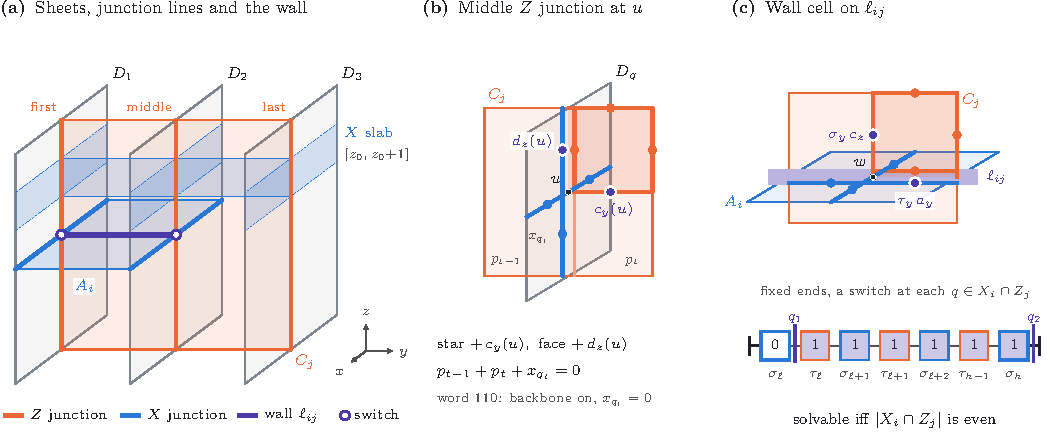
\includegraphics[width=\textwidth]{junction_wall_geometry.pdf}
\caption{Junction and wall geometry of the explicit realization.  (a) A
miniature instance with three data sheets $D_1,D_2,D_3$ (planes $y=Y_q$), one
$Z$-check sheet $C_j$ (plane $x=X_j$) with support $\{q_1,q_2,q_3\}$, and one
$X$-check sheet $A_i$ (plane $z=Z_i$) with support $\{q_1,q_2\}$.  The
$Z$ junctions are the $z$-lines where $C_j$ meets the data sheets (first,
middle, last), the $X$ junctions are the $x$-lines where $A_i$ meets them, and
the wall is the crossing line $\ell_{ij}$ of $C_j$ and $A_i$; its coefficients
switch at the two data qubits of $X_i\cap Z_j$.  A single-layer $X$ slab is
shaded.  (b) A middle $Z$ junction: the $D_q$ star at $u$ gains the $C_j$ edge
$c_y(u)$ and the $C_j$ face beside the line gains the data edge $d_z(u)$,
which enforces $p_{t-1}+p_t+x_{q_t}=0$ and lets the backbone pass an
unselected data sheet (word $110$).  (c) A wall cell on $\ell_{ij}$: the
$A_i$ star gains $\sigma_yc_z$ and the $C_j$ face gains $\tau_ya_y$; the
coefficients form a path with fixed ends, solvable exactly when
$|X_i\cap Z_j|$ is even.  The rules are listed in
Table~\ref{tab:explicit-junctions}.}
\label{fig:junction-geometry}
\end{figure*}

\begin{lemma}[Commuting checks and point defects]
\label{lem:explicit-commute}
With the junction rules, every star commutes with every face except possibly
an $A_i$ star on a crossing line $\ell_{ij}$ and a $C_j$ face adjacent to it.
For each crossing line the commutation conditions for these pairs are linear
in $(\sigma,\tau)$ and form a path
$\sigma_\ell,\tau_\ell,\sigma_{\ell+1},\dots,\tau_{h-1},\sigma_h$ whose two ends
are fixed.  The system has a solution, which is then unique, if and only if
$|\operatorname{supp}X_i\cap\operatorname{supp}Z_j|$ is even.  Hence, for every
CSS input, all checks commute.
\end{lemma}
\begin{proof}
Unmodified checks of one sheet commute as in the surface code, and checks of
different sheets share no qubit unless a rule added one.  It remains to
inspect the finitely many pairs touched by a rule.  (i) A $D$ star on a
$z$-line and a $C$ face containing $d_z$: their common qubits are $d_z$ and
the $C$ edge $c_y$ added to the star (or, at a first/last column, the shared
$z$-edge and the merged $C$ edge), two in each case.  (ii) An $A$ star on an
$x$-line and a $D$ face above that line: common qubits $d_z(u)$ and one
$a_x$ edge.  (iii) The added qubits $c_y$, $a_x$ lie in no other check of the
opposite type, so no further pair is affected.  (iv) An $A_i$ star on
$\ell_{ij}$ contains $d_z(u)$ when $u$ lies on a data line of $X_i$, and a
$C_j$ face contains $d_z$ of the same line when that data qubit is a middle
incidence of $Z_j$ (face on the $+y$ side) or its first/last incidence
(adjacent face through the shared column).  Hence the base overlap of such a
pair is $1$ exactly once for each common qubit $q\in X_i\cap Z_j$, and $0$
otherwise.  The wall additions change the overlap of the $A$ star at $y'$ and
the $C$ face on $[y,y+1]$, $y'\in\{y,y+1\}$, by $\sigma_{y'}+\tau_y$.  If the
$C$ face on $[\ell-1,\ell]$ exists it fixes $\sigma_\ell$; otherwise
$\ell$ is the first column of $C_j$, which is shared with a data line, and
commutation with the two $D$ faces adjacent to that line forces
$\sigma_\ell=0$; the right end is fixed in the same way.  Summing the path
equations telescopes to $\sigma_\ell+\sigma_h$ plus the sum of all base
overlaps, which is $|X_i\cap Z_j|$ modulo two.  A path with both ends fixed is
solvable exactly when this sum vanishes, and then uniquely.
\end{proof}

\begin{proposition}[The realization encodes exactly $K$ qubits]
\label{prop:explicit-k}
For every input CSS code with check weights at least two and every
$s\ge2$, the explicit realization is a CSS code with $k=K$.
\end{proposition}
\begin{proof}
\emph{Euler count.}  A data sheet has $L_x(L_z-1)+(L_x+1)L_z$ qubits,
$(L_x+1)(L_z-1)$ stars and $L_xL_z$ faces, so it contributes $+1$ to
$n-\#X-\#Z$.  A $C$ sheet of width $w$ has $w(L_z-1)$ $y$-edges,
$(w-1)L_z$ own $z$-edges, $(w-1)(L_z-1)$ stars and $wL_z$ faces, and an $A$
sheet of width $w$ has $L_x(w+1)+(L_x+1)w$ edges, $(L_x+1)(w+1)$ stars and
$L_xw$ faces; each contributes $-1$.  Junction and wall rules add no qubits
or checks.  Hence $n-\#X-\#Z=n_{\rm in}-m_X-m_Z$.

\emph{$X$ relations.}  Let $a$ be a set of stars whose product is the
identity.  Edges of $A_i$ lie only in the two $A_i$ stars at their ends, so
$a$ is constant, $\alpha_i$, on the stars of $A_i$.  On the data column
$x=0$ of $D_q$, the edge $d_z(0,Y_q,z)$ lies in the $D_q$ stars at its ends
(when present) and, for $z=Z_i$ with $q\in X_i$, in one $A_i$ star; the rows
$z=0,L_z$ carry no stars.  Summing along the column gives
$\sum_{i\ni q}\alpha_i=0$, i.e.\ $\alpha^TH_X=0$.  Conversely $\alpha$
determines $a$: the $D$ stars are determined column by column from $z=0$ and
are constant along rows (a $D$ $x$-edge lies only in the two stars at its
ends), and the $C$ stars are determined column by column from $z=0$, where
$c_z(y,0)$ lies in a single star.  Thus the space of $X$ relations injects
into the left kernel of $H_X$.

\emph{$Z$ relations.}  Let $b$ be a set of faces with trivial product.  The
edges of $C_j$ lie only in $C_j$ faces, two each, so $b$ is constant,
$\gamma_j$, on $C_j$.  A $D$ $x$-edge lies only in the faces above and below
it, so $b$ is constant, $\beta_q(x)$, on each column of faces of $D_q$.  A
data $z$-edge at column $x$ lies in the $D$ faces at $x-1$ and $x$ and, for
$x=X_j$ with $q\in Z_j$, in one $C_j$ face; the edges at $x=0$ and $x=L_x$ lie
in one face.  Hence $\beta_q(0)=\beta_q(L_x-1)=0$ and
$\beta_q(x-1)+\beta_q(x)=\sum_{j:X_j=x,\,q\in Z_j}\gamma_j$, which sum to
$\gamma^TH_Z=0$.  The $A$ faces are determined by $\gamma$ from the column
$x=0$, where each $a_y$ lies in one face.  So the $Z$ relations inject into the
left kernel of $H_Z$.

Therefore, writing $H_X^{\rm lc},H_Z^{\rm lc}$ for the check matrices of the explicit realization, $k=n-\rank H_X^{\rm lc}-\rank H_Z^{\rm lc}
=(n-\#X-\#Z)+\dim(\text{relations})\le
n_{\rm in}-\rank H_X-\rank H_Z=K$.  Theorem~\ref{thm:slab-resolved} below
exhibits $K$ independent logical pairs, so $k=K$.
\end{proof}

\paragraph{Prefix-parity slab operators.}
For $x\in\ker H_Z$ and a height $0\le z_0<L_z$ let
\begin{align}
 \widetilde X(x;z_0)&=\sum_q x_q\,E^D_q(z_0)
 +\sum_j\sum_{t=1}^{k_j-1}p^{(j)}_t\,E^C_{j,t}(z_0),\nonumber\\
 p^{(j)}_t&=\sum_{h=1}^{t}x_{q^{(Z_j)}_h},
 \label{eq:prefix-backbone}
\end{align}
where $E^D_q(z_0)$ is the set of $D_q$ $z$-edges spanning $[z_0,z_0+1]$
(all $x$), and $E^C_{j,t}(z_0)$ is the set of $C_j$-owned $z$-edges
spanning $[z_0,z_0+1]$ with $Y_{q_t}<y\le Y_{q_{t+1}}$, excluding a shared
last column.  Commutation of $x$ with $Z_j$ is
\begin{equation}
 \sum_{t=1}^{k_j}x_{q_t}=0\pmod 2,
 \label{eq:check-even-parity}
\end{equation}
so $p^{(j)}_{k_j}=0$ and $p_{t-1}+p_t+x_{q_t}=0$ at every incidence
($p_0=0$), i.e., with $H_{\rm end}=[1\;1]$ and $H_{\rm mid}=[1\;1\;1]$
(Eq.~\eqref{eq:H-end}),
\begin{align}
 (p_{t-1},p_t,x_{q_t})&\in\ker H_{\rm mid},\nonumber\\
 (p_1,x_{q_1}),\,(p_{k-1},x_{q_k})&\in\ker H_{\rm end}.
 \label{eq:local-prefix-parity}
\end{align}
Dually, for $z\in\ker H_X$ and a column $0\le x_0\le L_x$ let
$\widetilde Z(z;x_0)$ be $Z$ on the $D_q$ $z$-edges of column $x_0$ (all $z$)
for $z_q=1$, and on the $A_i$ $y$-edges of column $x_0$ with
$Y_{q_t}\le y<Y_{q_{t+1}}$ for $r^{(i)}_t=\sum_{h\le t}z_{q_h^{(X_i)}}=1$.

\begin{theorem}[Single-layer slab representatives]
\label{thm:slab-resolved}
In the explicit realization, for every height $z_0$ and every column $x_0$:
\begin{enumerate}
\item \emph{(gluing forms)} for every face $h$, the overlap parity
$\langle h,\widetilde X(x;z_0)\rangle$ is either $0$ or exactly one of the
linear forms $x_{q_1}+p_1$, $p_{t-1}+p_t+x_{q_t}$, $p_{k-1}+x_{q_k}$ of a
single incidence of a single check; each such form occurs.  The dual
statement holds for stars and $\widetilde Z(z;x_0)$;
\item $\widetilde X(x;z_0)$ commutes with every stabilizer for all
$x\in\ker H_Z$, and $\widetilde Z(z;x_0)$ for all $z\in\ker H_X$;
\item $\langle\widetilde X(x;z_0),\widetilde Z(z;x_0)\rangle=x\cdot z$;
\item every pure-$X$ logical class has a representative supported on the
single layer of $z$-edges spanning $[z_0,z_0+1]$, and every pure-$Z$ logical
class has one in the plane $x=x_0$.
\end{enumerate}
\end{theorem}
\begin{proof}
(1) A face meets the edges of $\widetilde X$ only if it is a $D$ face or a
$C$ face in the row $[z_0,z_0+1]$; $A$ faces contain only $A$ edges.  A
$D$ face there contains two $z$-edges of the same data string, and the qubit
$a_x$ added above an $x$-line is not in $\widetilde X$; its form is $0$.  A
$C$ face on $[y,y+1]$ contains the $C_j$ columns $y$ and $y+1$.  Inside a
segment both carry $p_t$; the wall qubit $a_y$ is not in $\widetilde X$.  At a
middle incidence $q_t$ the $+y$ face contains the line edge $c_z(Y_{q_t})$,
which belongs to the segment ending there and carries $p_{t-1}$, the next
column ($p_t$) and the added $d_z$ ($x_{q_t}$).  At the first (last)
incidence the face adjacent to the shared column contains that data edge
($x_{q_1}$, resp.\ $x_{q_k}$) and one segment column.  Each incidence
therefore contributes exactly one face per height.  The dual argument uses
the $D$ stars of column $x_0$ (two consecutive data edges, and $c_y$ not in
$\widetilde Z$) and the $A$ stars of column $x_0$, whose added edge
$d_z(u)$ carries $z_q$ at an incidence row; the wall qubit $c_z$ is not in
$\widetilde Z$.  (2) follows from (1) and
Eq.~\eqref{eq:local-prefix-parity}.  (3) The $C$ edges of $\widetilde X$ and
the $A$ edges of $\widetilde Z$ are disjoint, and the data strings meet in the
single edge $d_z(x_0,Y_q,z_0)$ for each $q$ with $x_q=z_q=1$.  (4) Applied to a
symplectic basis of the input code, (2)--(3) give $K$ independent logical
pairs.  By Proposition~\ref{prop:explicit-k} they exhaust the logical space,
so $x\mapsto[\widetilde X(x;z_0)]$ maps $\ker H_Z$ onto the pure-$X$
logical classes; an $x$ in the row space of $H_X$ pairs trivially with every
$\widetilde Z$ and is therefore mapped to a stabilizer.  The same holds for
$\widetilde Z$.
\end{proof}

The support of $\widetilde X(x;z_0)$ is a single layer of $z$-edges, so the
slab thickness is $t_0=1$, and $\widetilde Z(z;x_0)$ lies in one plane.  No
admissibility condition on $z_0$ or $x_0$ is needed: the construction works
on check layers as well as between them, because the wall rules add only
qubits that the slab operators do not use, the $Z$-junction rules are the same
at every height and the $X$-junction rules the same at every column, and the
remaining junction rules ($X$ junctions for $\widetilde X$, $Z$ junctions for
$\widetilde Z$) add only qubits that the slab operator does not use.

\begin{corollary}[Uniform-gap slab mobility]
\label{cor:uniform-gap-slabs}
For a balanced input family with $m_X,m_Z=\Theta(N)$, there are
\begin{equation}
 r_X=L_z=\Theta(N),\qquad r_Z=L_x+1=\Theta(N)
 \label{eq:many-slabs-count}
\end{equation}
pairwise disjoint complete $X$ ports (one per height) and complete $Z$ ports
(one per column).
\end{corollary}

\begin{lemma}[Locality of the explicit realization]
\label{lem:wb-cell-locality}
Every check of the explicit realization is supported within the unit
$L^\infty$ ball of one lattice vertex, has weight at most six, and every qubit lies in at most three checks
of each type; at most two qubits share a lattice edge.  These bounds are
independent of the input code, of $s$, and of the block size.
\end{lemma}
\begin{proof}
Stars have at most four in-sheet edges, plus at most one junction qubit and,
for $A$ stars, one wall qubit; faces have at most four edges plus at most one
junction qubit and one wall qubit.  All added qubits are edges at the same vertex, or edges of the same face
position, as the check they join.  A
data line edge lies in two data faces and at most one $C$ face; an $a_x$ edge
lies in two $A$ faces and at most one $D$ face; the remaining edge types are
counted in the same way.  Two sheets meet along a line, so at most two qubits
share an edge.
\end{proof}

\begin{theorem}[Distance of the explicit realization]
\label{thm:explicit-distance}
Let $d_X^{\rm in},d_Z^{\rm in}$ be the distances of the input code,
$w_X,w_Z$ its largest $X$- and $Z$-check weights, and
\begin{equation}
 \eta_X=\max\{1,\lfloor w_X/2\rfloor\},\qquad
 \eta_Z=\max\{1,\lfloor w_Z/2\rfloor\}.
 \label{eq:eta}
\end{equation}
The explicit realization has
\begin{equation}
 d_X\ge(L_x+1)\left\lceil\frac{d_X^{\rm in}}{\eta_X}\right\rceil,\qquad
 d_Z\ge L_z\left\lceil\frac{d_Z^{\rm in}}{\eta_Z}\right\rceil,
 \label{eq:explicit-distance}
\end{equation}
and, from the slab representatives of a minimum-weight input logical,
$d_X\le(L_x+1)d_X^{\rm in}+s\,m_Zn_{\rm in}$ and
$d_Z\le L_zd_Z^{\rm in}+s\,m_Xn_{\rm in}$.
For a balanced good input family with bounded check weight,
$d_X,d_Z=\Theta(N^2)$.
\end{theorem}
\begin{proof}
Let $O$ be a nontrivial $X$-type logical.  By Theorem~\ref{thm:slab-resolved}
the $\widetilde X(x;z_0)$ represent every $X$ class, so $O$ is equivalent to
some $\widetilde X(x;z_0)$ with $x\in\ker H_Z$ outside the row space of $H_X$,
and $\langle O,\widetilde Z(z;x_0)\rangle=x\cdot z$ for every $z\in\ker H_X$ and
every column $x_0$.  Fix $x_0$.  The support of $\widetilde Z(z;x_0)$ is a union
of disjoint pieces lying in the plane $x=x_0$: the data column of $D_q$ when
$z_q=1$ and the column-$x_0$ segment $t$ of $A_i$ when
$r^{(i)}_t=\sum_{h\le t}z_{q_h}=1$.  Let $a_q$ and $b_{i,t}$ be the parities of
$O$ on these pieces.  Then
\begin{align*}
 \langle O,\widetilde Z(z;x_0)\rangle&=\sum_q z_qa_q+\sum_{i,t}r^{(i)}_tb_{i,t}
 =z\cdot v(x_0),\\
 v(x_0)&=\sum_q a_q e_q+\sum_{i,t}b_{i,t}\,\pi_{i,t},
\end{align*}
where $\pi_{i,t}$ is the indicator of the \emph{prefix}
$\{q^{(X_i)}_1,\ldots,q^{(X_i)}_t\}$ of check $X_i$.  Since
$z\cdot v(x_0)=z\cdot x$ for all $z\in\ker H_X$, the vector $v(x_0)$ lies in
$x+\operatorname{row}H_X$.  For a check of weight $k$, the prefix $\pi_{i,t}$
and the complementary suffix $\pi_{i,t}+X_i$ differ by the row $X_i$ of $H_X$,
and the shorter of the two has at most $\min\{t,k-t\}\le\lfloor k/2\rfloor$
entries.  Replace every occupied prefix by its shorter side:
\begin{equation*}
 v'(x_0)=\sum_q a_q e_q+\sum_{i,t}b_{i,t}\,\pi'_{i,t},\qquad
 \pi'_{i,t}\in\{\pi_{i,t},\pi_{i,t}+X_i\}.
\end{equation*}
This adds a sum of rows of $H_X$, so $v'(x_0)\in x+\operatorname{row}H_X$ is
still a nontrivial $X$ logical of the input code and $|v'(x_0)|\ge d_X^{\rm in}$.
Each nonzero $a_q$ contributes one entry of $v'(x_0)$ and each nonzero
$b_{i,t}$ at most $\eta_X$ entries, so the number of pieces of odd parity is
an integer of at least $d_X^{\rm in}/\eta_X$, hence at least
$\lceil d_X^{\rm in}/\eta_X\rceil$, and each such piece contains a qubit of
$O$.  The planes $x=x_0$, $0\le x_0\le L_x$, are disjoint; summing the integer
bound over them gives $|O|\ge(L_x+1)\lceil d_X^{\rm in}/\eta_X\rceil$.  The $Z$
bound is the same argument with the layers of $z$-edges at the heights
$0\le z_0<L_z$, the $X$ slabs, and the prefixes of the $Z$ checks.  The upper
bounds count the data strings of a minimum-weight input logical and at most
$s\,n_{\rm in}$ backbone edges per check.  For balanced good inputs,
$L_x,L_z=\Theta(N)$ and $d^{\rm in}=\Theta(N)$.
\end{proof}

The argument lifts the input distance through the complete ports of
Theorem~\ref{thm:slab-resolved}: each of the $\Theta(N)$ disjoint planes of one
orientation must carry a whole input logical's worth of the operator.  Two
features give the constant.  A backbone piece represents a prefix of a check,
which may be exchanged for the complementary suffix modulo that check, so a
piece costs at most half a check weight; and the count of occupied pieces is
rounded up in each plane before summing over planes.  The script \texttt{distance\_lower\_bound\_check.py} checks each step on every
input of Table~\ref{tab:slab-certificate} up to $n_{\rm in}=15$.  Every basis
slab is exactly the union of the pieces used above, lies in its own plane or
layer, and obeys the upper bound ($1010$ slabs).  For random representatives
(slab operators times random stabilizers) at every column and height ($3858$
cases), both $v(x_0)$ and its shortest-side replacement $v'(x_0)$ land in the
right coset, $|v'(x_0)|$ is at most $\eta$ times the number of occupied pieces,
and that number is at least $\lceil d^{\rm in}/\eta\rceil$.  The script also
compares Eq.~\eqref{eq:explicit-distance} with the exact distances of
Table~\ref{tab:explicit-distance}.  For the inputs $[[4,2,2]]$ and $[[6,4,2]]$
($d^{\rm in}=2$, $\eta=2$ and $3$) the bound is $d_X\ge L_x+1$,
$d_Z\ge L_z$, and it equals the exact distance in every instance.  At $s=5$,
where the CP-SAT search stopped at the brackets $10$--$11$ and $9$--$10$, the
theorem closes them: $d_X=11$ and $d_Z=10$.  For an input of distance three
the exact comparison is still open.  For the Steane $[[7,1,3]]$ input at $s=2$
($n=1792$, $\eta=2$) the bound is $d_X\ge18$ and $d_Z\ge16$; two hours of
CP-SAT per sector bracket $d_X$ between $14$ and $20$ and $d_Z$ between $14$
and $19$ (\texttt{run\_distances.py} in \nolinkurl{scaling_campaign/campaign/},
\nolinkurl{numerical/scaling_campaign/code_distance.csv}).  The search found
no logical operator lighter than the bound.

\begin{table}[t]
\caption{Code-capacity distances of the explicit realization
(\texttt{explicit\_layer\_code\_distance.py}).  The upper bound is an explicit
undetectable logical found by Stim's search, the lower bound is proved with
CP-SAT, and the last two columns give the bound of
Theorem~\ref{thm:explicit-distance}.  At $s=5$ the CP-SAT bounds are $10$ and
$9$, and the theorem supplies the matching lower bounds ($^\dagger$).}
\label{tab:explicit-distance}
\centering
\small
\begin{tabular}{@{}lrrrrrrr@{}}
\toprule
Input & $s$ & $n$ & $L_x=L_z$ & $d_X$ & $d_Z$ & \multicolumn{2}{c}{Eq.~\eqref{eq:explicit-distance}} \\
\midrule
$[[4,2,2]]$ & 2 & 224 & 4 & 5 & 4 & 5 & 4 \\
$[[4,2,2]]$ & 3 & 504 & 6 & 7 & 6 & 7 & 6 \\
$[[4,2,2]]$ & 4 & 896 & 8 & 9 & 8 & 9 & 8 \\
$[[4,2,2]]$ & 5 & 1400 & 10 & $11^\dagger$ & $10^\dagger$ & 11 & 10 \\
$[[6,4,2]]$ & 2 & 352 & 4 & 5 & 4 & 5 & 4 \\
$[[6,4,2]]$ & 3 & 792 & 6 & 7 & 6 & 7 & 6 \\
$[[6,4,2]]$ & 4 & 1408 & 8 & 9 & 8 & 9 & 8 \\
\bottomrule
\end{tabular}
\end{table}

\begin{lemma}[Symplectic correspondence]
\label{lem:slab-symplectic-resolved}
For the representatives of Theorem~\ref{thm:slab-resolved},
$\langle\widetilde X(a;z_0),\widetilde Z(b;x_0)\rangle=a\cdot b\pmod 2$ for
all heights and columns.
\end{lemma}
\begin{proof}
This is item (3) of Theorem~\ref{thm:slab-resolved}.
\end{proof}

\paragraph{Why the slab theorem is the bottleneck.}
The middle-junction relation $p_{t-1}+p_t+x_{q_t}=0$ is the nontrivial local
move: it lets backbone parity cross an unselected data sheet ($110$) without
creating a companion string.  A realization that enforces only the
all-equal relation at middle junctions cannot represent a general logical in
a slab, and indeed does not encode the input logical qubits
(Sec.~\ref{sec:certificate}).

\subsection{Relation to the published junction cells}
\label{app:source-trace}

\paragraph{Condensation data.}
WB specify each line junction by condensed anyon generators.  For the first
$\hat z$ junction, with $m$-occupations $(p,x_L,x_R)$ of the check sheet and
the two sides of the data sheet, the condensed $e$ generators
$e_{C}e_{D_1}$ and $e_{D_1}e_{D_2}$ give, by trivial braiding,
\begin{equation}
 G_{\rm end}=\begin{bmatrix}1&1&0\\0&1&1\end{bmatrix},
 \label{eq:source-end}
\end{equation}
and for a through-going data string ($x_L=x_R$) the relation
$H_{\rm end}=[1\;1]$.  For a middle junction with occupations
$(p_L,p_R,x_L,x_R)$ the generators $e_{C_1}e_{C_2}e_{D_1}$ and
$e_{D_1}e_{D_2}$ give
\begin{equation}
 G_{\rm mid}=\begin{bmatrix}1&1&1&0\\0&0&1&1\end{bmatrix},
 \label{eq:source-mid}
\end{equation}
and $H_{\rm mid}=[1\;1\;1]$.  Thus
\begin{align}
 H_{\rm end}&=\begin{bmatrix}1&1\end{bmatrix}, &
 \ker H_{\rm end}&=\{00,11\},\nonumber\\
 H_{\rm mid}&=\begin{bmatrix}1&1&1\end{bmatrix}, &
 \ker H_{\rm mid}&=\{000,110,101,011\}.
 \label{eq:H-end}
\end{align}
The $X$-check junctions are the $X\leftrightarrow Z$ duals.  The condensed
anyons of the explicit junctions (Table~\ref{tab:explicit-junctions}) are
exactly these data: at a middle $\hat z$ junction, $Z$ on the two data edges
across the line passes through the star ($e_{D_1}e_{D_2}$); $Z$ on the two
$C$ edges across the line leaves one violation of the data star, which carries
$c_y$ ($e_{C_1}e_{C_2}e_D$); $X$ on the $C$ line edge flips the two $C$ faces
beside it ($m_{C_1}m_{C_2}$, the $110$ pass-through); and $X$ on the data line
edge flips the two data faces and the $+y$ $C$ face ($m_{C_2}m_{D_1}m_{D_2}$).
The first and last junctions, where $C_j$ shares the data line, condense all
$e$ pairs and $m_Cm_{D_1}m_{D_2}$.  Each set generates a Lagrangian subgroup
of the four (three) incident half-sheets.

\paragraph{The single-chart transcription (negative control).}
A transcription of WB Sec.~VI~B items 3--8 into one unit-cubic chart
(Table~\ref{tab:wb-support}) lets the check sheet and the data sheet share the
line edges and makes every junction star the union of the two sheet stars.
Glued, these cells form the plain union of the sheets.
At a middle junction the plain union condenses every $e$ pair and only the
fourfold $m$ product, so a slab operator must satisfy $p_{t-1}=p_t=x_{q_t}$:
the all-equal relation $\{000,111\}$, not $\ker H_{\rm mid}$.  The complete
single-chart codes do not encode $K$ qubits (Table~\ref{tab:slab-certificate}),
which makes the transcription a useful negative control (an earlier version
of this work used it, with a certificate that did not detect the problem;
Sec.~\ref{sec:archive}).  The transcription's ``novel'' $S^Z$ entries
($P^+_{yz}$ at middle $\hat z$ cells, $P^+_{xz}$ at $\hat x$ cells) are exactly
the faces that, in the explicit realization, carry the other sheet's line
edge.  This suggests that the published cells use two sheets with distinct
line qubits, as the explicit realization does.  We do not claim literal
identity with the published drawings; the theorem above is stated for the
explicit realization, whose complete check matrices are generated by
\texttt{layer\_code\_explicit.py}.

\begin{table*}[t]
\caption{Single-chart unit-cubic transcription of the novel WB Sec.~VI~B
line-junction checks, kept as the negative control of
Sec.~\ref{sec:certificate}; the explicit realization of
Sec.~\ref{sec:explicit-realization} replaces it.  A
dash means that no additional check of that type is listed.}
\label{tab:wb-support}
\renewcommand{\arraystretch}{1.12}
\scriptsize
\begin{tabular}{@{}c p{2.3cm} p{6.0cm} p{5.6cm}@{}}
\toprule
Source item & Cell & Novel $S^X$ support & Novel $S^Z$ support \\
\midrule
3 & first $\hat z$ & $\{q_{x-},q_{x+},q_{y+},q_{z-},q_{z+}\}$ & --- \\
4 & middle $\hat z$ & $\{q_{x-},q_{x+},q_{y-},q_{y+},q_{z-},q_{z+}\}$ & $P_{yz}^{+}$ \\
5 & last $\hat z$ & $\{q_{x-},q_{x+},q_{y-},q_{z-},q_{z+}\}$ & --- \\
6 & first $\hat x$ & $\{q_{x-},q_{x+},q_{y+},q_{z-},q_{z+}\}$ & $P_{xz}^{+}$ \\
7 & middle $\hat x$ & $\{q_{x-},q_{x+},q_{y-},q_{y+},q_{z-},q_{z+}\}$ & $P_{xz}^{+}$ \\
8 & last $\hat x$ & $\{q_{x-},q_{x+},q_{y-},q_{z-},q_{z+}\}$ & $P_{xz}^{+}$ \\
\bottomrule
\end{tabular}
\end{table*}

\paragraph{Microscopic inputs.}
Table~\ref{tab:slab-inputs} lists every local input of
Theorem~\ref{thm:slab-resolved} and its status.

\begin{table*}[t]
\caption{Local inputs to Theorem~\ref{thm:slab-resolved} and their status.}
\label{tab:slab-inputs}
\scriptsize
\setlength{\tabcolsep}{3.0pt}
\renewcommand{\arraystretch}{1.18}
\begin{tabular}{@{}p{3.6cm}p{5.2cm}p{7.2cm}@{}}
\toprule
Input & Status & Where it is used \\
\midrule
Sheet surface codes and boundaries & Defined here (Sec.~\ref{sec:explicit-realization}) & Euler count, relation injectivity, slab strings \\
$Z$/$X$ line-junction rules & Defined here (Table~\ref{tab:explicit-junctions}); condensation data equal to WB's (Sec.~\ref{app:source-trace}) & Gluing forms, $k=K$ \\
Wall rules at crossing lines & Derived here (Lemma~\ref{lem:explicit-commute}); solvable iff input commutes & Commutation of all checks \\
$H_{\rm end}$, $H_{\rm mid}$ & Derived from WB condensation generators (Eqs.~\eqref{eq:source-end}--\eqref{eq:H-end}); realized by one face per incidence and height (Theorem~\ref{thm:slab-resolved}(1)) & Prefix recurrence \\
Prefix-parity assembly & Proved here (Eqs.~\eqref{eq:prefix-backbone}--\eqref{eq:local-prefix-parity}) & Every pure logical class \\
$k=K$ & Proved here (Proposition~\ref{prop:explicit-k}) & Completeness of the slab representatives \\
$d=\Theta(N^2)$ & Proved here (Theorem~\ref{thm:explicit-distance}); exact small-instance values in Table~\ref{tab:explicit-distance} & Architecture theorem only \\
Complete finite certificate & \texttt{slab\_gluing\_certificate.py} (Sec.~\ref{sec:certificate}) & Independent check of all of the above on finite inputs \\
\bottomrule
\end{tabular}
\end{table*}

\begin{lemma}[Interface inputs for the slab theorem]
\label{lem:interface-completeness}
Theorem~\ref{thm:slab-resolved} uses only the sheet definitions, the
junction and wall rules of Table~\ref{tab:explicit-junctions}, and
Proposition~\ref{prop:explicit-k}; it uses no property of the published
lattice drawings and no finite certificate.
\end{lemma}
\begin{proof}
Every step of the proof of Theorem~\ref{thm:slab-resolved} is a statement
about the checks meeting one layer of $z$-edges (or one column), and these
checks are listed in Table~\ref{tab:explicit-junctions}.
\end{proof}

\paragraph{Port separation and constant refinement.}
The gauging construction of Sec.~\ref{sec:gauging} maps distinct port qubits
to distinct grid vertices.  At most two qubits share a lattice edge
(Lemma~\ref{lem:wb-cell-locality}), so a grid of twice the lattice resolution
separates them, changing the grid constants and the port thickness $t$ by
$O(1)$; the two-block simulation of Sec.~\ref{sec:two-block} uses exactly this
map.  The slab theorem itself needs no refinement.  The stabilizer-equivalent
subdivisions below remain available for enlarging ordinary sheet regions.

\begin{lemma}[Constant subdivision refinement is stabilizer equivalent]\label{lem:constant-refinement}
Fix a refinement factor $c$.  Let $\mathcal S$ be the stabilizer group before refinement and let $\mathcal A_c$ be the product-state stabilizers of the finitely many new $|+\rangle$ and $|0\rangle$ edge qubits.  The subdivision refinement admits a geometrically local Clifford circuit $U_c$ of depth and light-cone size depending only on $c$ and the finite local catalog such that
\begin{equation*}
 \mathcal S_{\rm ref}=U_c(\mathcal S\otimes\mathcal A_c)U_c^\dagger .\tag{R1}
\end{equation*}
Consequently the encoded logical dimension is exactly unchanged.  If $s_c$ bounds the Pauli light-cone size of both $U_c$ and $U_c^\dagger$, then
\begin{equation*}
 \frac{d}{s_c}\le d_{\rm ref}\le s_c d .\tag{R2}
\end{equation*}
\end{lemma}
\begin{proof}
For an edge split, add $a$ in $|+\rangle$ and apply $U_E=\mathrm{CNOT}_{a\to q}$, so that $X_a\mapsto X_aX_q$ and $Z_q\mapsto Z_aZ_q$: the first image is the new degree-two star, and every face containing $q$ acquires $Z_aZ_q$.  For a face split along paths $P_1,P_2$, add $a$ in $|0\rangle$ and apply $\prod_{q\in P_1}\mathrm{CNOT}_{q\to a}$, so that $Z_a\mapsto Z_aZ(P_1)$ and the two refined faces are generated; in the $X$ sector each endpoint star of $P_1$ acquires $X_a$.  Bounded-degree moves are colored into $O_c(1)$ layers.  Local Clifford equivalence with initialized ancillas preserves $K$, and light cones give (R2).
\end{proof}


\subsection{Symplectic overlap of transverse logical ports}
\label{sec:symplectic-overlap}
The fixed slabs expose not only local representatives but also a quantitative
constraint on how two logical polarizations can overlap.  For an $[[n,K]]$
CSS code, let
\begin{align}
 \mathcal L_X&=\ker H_Z/\operatorname{row}H_X,\\
 \mathcal L_Z&=\ker H_X/\operatorname{row}H_Z,
\end{align}
so $\dim\mathcal L_X=\dim\mathcal L_Z=K$ and the physical dot product induces
a perfect bilinear commutation pairing
$\langle\cdot,\cdot\rangle:\mathcal L_X\times\mathcal L_Z\to\mathbb F_2$.
For a physical region $R$, define $\mathcal X(R)\subseteq\mathcal L_X$ and
$\mathcal Z(R)\subseteq\mathcal L_Z$ to be the logical classes admitting,
respectively, pure-$X$ and pure-$Z$ representatives supported in $R$, and set
\begin{equation}
 g_X(R)=\dim\mathcal X(R),\qquad g_Z(R)=\dim\mathcal Z(R).
 \label{eq:gxgz-def}
\end{equation}
For two regions $A,B$, write
\begin{equation}
 r(A,B)=\rank\!\left(\langle\cdot,\cdot\rangle
 \big|_{\mathcal X(A)\times\mathcal Z(B)}\right).
 \label{eq:overlap-rank-def}
\end{equation}

\begin{theorem}[Overlap-corrected CSS cleaning inequality]
\label{thm:overlap-cleaning}
For every pair of physical regions $A,B$ in an $[[n,K]]$ CSS stabilizer code,
\begin{equation}
 \max\{0,g_X(A)+g_Z(B)-K\}\le r(A,B)\le |A\cap B|,
 \label{eq:overlap-rank-sandwich}
\end{equation}
and therefore
\begin{equation}
 g_X(A)+g_Z(B)\le K+|A\cap B|.
 \label{eq:overlap-cleaning}
\end{equation}
\end{theorem}

\begin{proof}
Put $C=A\cap B$, $a=g_X(A)$, and $b=g_Z(B)$.  Choose bases of the two
supported logical spaces and pure representatives $x_i\subseteq A$ and
$z_j\subseteq B$.  Their logical commutation matrix has entries
$M_{ij}=x_i\cdot z_j$.  Outside $C$, at least one factor vanishes, so if
$X_C\in\mathbb F_2^{a\times|C|}$ and
$Z_C\in\mathbb F_2^{b\times|C|}$ collect the restrictions, then
$M=X_CZ_C^T$ and hence $r(A,B)=\rank M\le|C|$.

For the lower bound, put $U=\mathcal X(A)$ and $V=\mathcal Z(B)$.  The kernel
of the restricted pairing map $U\to V^*$ is $U\cap V^\perp$.  Because the full
$X/Z$ logical pairing is nondegenerate, $\dim V^\perp=K-b$, and therefore
\begin{equation*}
 r(A,B)=a-\dim(U\cap V^\perp)\ge a-(K-b)=a+b-K.
\end{equation*}
Combining this with nonnegativity gives Eq.~\eqref{eq:overlap-rank-sandwich},
and the upper and lower bounds together give Eq.~\eqref{eq:overlap-cleaning}.
\end{proof}

For $B=A^c$, the overlap penalty vanishes.  The usual stabilizer cleaning lemma sharpens the resulting inequality to the familiar complementary-region identity in the appropriate logical sectors \cite{HaahPreskillTradeoff}.  Equation~\eqref{eq:overlap-cleaning} is useful here because it applies to arbitrary overlapping regions.

\begin{theorem}[Port-packing inequality]
\label{thm:port-packing}
Let $A_1,\ldots,A_r$ and $B$ be physical regions of an $[[n,K]]$ CSS code.  Suppose each physical qubit belongs to at most $c$ of the regions $A_i$.  Then
\begin{equation}
 \sum_{i=1}^r g_X(A_i)
 \le r\bigl(K-g_Z(B)\bigr)+c|B| .
 \label{eq:port-packing-general}
\end{equation}
If $B$ is a complete pure-$Z$ port, $g_Z(B)=K$, this reduces to
\begin{equation}
 \sum_{i=1}^r g_X(A_i)\le c|B| .
 \label{eq:port-packing-complete}
\end{equation}
For pairwise-disjoint $A_i$, $c=1$.  If in addition every $A_i$ is a complete pure-$X$ port, then
\begin{equation}
 rK\le |B| .
 \label{eq:port-packing-complete-ports}
\end{equation}
The $X\leftrightarrow Z$ statement holds by duality.
\end{theorem}

\begin{proof}
Apply Theorem~\ref{thm:overlap-cleaning} to each pair $(A_i,B)$:
\begin{equation*}
 g_X(A_i)\le K-g_Z(B)+|A_i\cap B|.
\end{equation*}
Summing and counting the intersections qubit by qubit gives
\begin{equation*}
 \sum_i |A_i\cap B|
 =\sum_{q\in B}\#\{i:q\in A_i\}\le c|B|,
\end{equation*}
which proves Eq.~\eqref{eq:port-packing-general} and its special cases.
\end{proof}

The complete-$B$ case also has a direct proof that does not rely on choosing mutually compatible representatives.  Put $U_i=\mathcal X(A_i)$ and $C_i=A_i\cap B$.  Choose a basis of $U_i$, choose one pure-$X$ representative supported in $A_i$ for each basis vector, and extend linearly.  Restricting this representative map to $C_i$ gives
\begin{equation*}
 \rho_i:U_i\longrightarrow \mathbb F_2^{C_i}.
\end{equation*}
If $\rho_i(u)=0$, the chosen representative of $u$ is disjoint from $B$.  Because $g_Z(B)=K$, every pure-$Z$ logical class has a representative in $B$, so $u$ commutes with the entire $Z$-logical space.  Nondegeneracy of the CSS logical pairing forces $u=0$.  Thus $\rho_i$ is injective and $g_X(A_i)\le |C_i|$.  Summing gives Eq.~\eqref{eq:port-packing-complete} directly.

\begin{theorem}[Symplectic crossbar bound]
\label{thm:symplectic-crossbar}
Let $A_1,\ldots,A_r$ and $B_1,\ldots,B_s$ be physical regions of an
$[[n,K]]$ CSS code.  Suppose each physical qubit belongs to at most $c_X$ of
the regions $A_i$ and at most $c_Z$ of the regions $B_j$.  Put
$a_i=g_X(A_i)$ and $b_j=g_Z(B_j)$.  Then
\begin{equation}
 \sum_{i=1}^r\sum_{j=1}^s
 \max\{0,a_i+b_j-K\}
 \le \sum_{i=1}^r\sum_{j=1}^s r(A_i,B_j)
 \le c_Xc_Z n .
 \label{eq:crossbar-general}
\end{equation}
In particular, if every $A_i$ is a complete pure-$X$ port and every $B_j$
is a complete pure-$Z$ port, then
\begin{equation}
 rsK\le c_Xc_Z n.
 \label{eq:crossbar-complete}
\end{equation}
For pairwise-disjoint families, $c_X=c_Z=1$ and hence
\begin{equation}
 rsK\le n.
 \label{eq:crossbar-disjoint}
\end{equation}
\end{theorem}

\begin{proof}
Theorem~\ref{thm:overlap-cleaning} gives, for every pair $(i,j)$,
\begin{equation*}
 \max\{0,a_i+b_j-K\}\le r(A_i,B_j)\le |A_i\cap B_j|.
\end{equation*}
For a physical qubit $q$, set
$\mu_X(q)=\#\{i:q\in A_i\}$ and $\mu_Z(q)=\#\{j:q\in B_j\}$.  Summing the
intersection sizes and then counting qubitwise gives
\begin{equation*}
 \sum_{i,j}|A_i\cap B_j|
 =\sum_q \mu_X(q)\mu_Z(q)
 \le c_Xc_Zn,
\end{equation*}
which proves Eq.~\eqref{eq:crossbar-general}.  The complete-port and
disjoint-family statements follow immediately.
\end{proof}

\begin{definition}[CSS symplectic-overlap number]
\label{def:chi-xz}
Define
\begin{equation}
 \chi_{XZ}(Q)=\min_{\substack{A,B:\\ g_X(A)=K,\;g_Z(B)=K}}|A\cap B|.
 \label{eq:chi-xz}
\end{equation}
Thus $\chi_{XZ}$ is the smallest physical intersection through which a complete pure-$X/Z$ logical polarization can realize its full commutation pairing.  Theorem~\ref{thm:overlap-cleaning} gives
\begin{equation}
 \chi_{XZ}(Q)\ge K.
 \label{eq:chi-lower}
\end{equation}
\end{definition}

\begin{corollary}[Layer-code crossbar saturation and transverse rank]
\label{cor:layer-port-packing}
For the balanced layer-code family (explicit realization), choose
$r_X=\Theta(N)$ pairwise-disjoint complete $X$ slabs
$A_1,\ldots,A_{r_X}$ and $r_Z=\Theta(N)$ pairwise-disjoint complete $Z$ slabs
$B_1,\ldots,B_{r_Z}$.  Then, for every $i,j$,
\begin{align}
 r_XK&\le |B_j|=\Theta(N^2)=\Theta(K^2),
 \label{eq:layer-port-pack}\\
 r(A_i,B_j)&=K,\qquad |A_i\cap B_j|=\Theta(K),
 \label{eq:layer-crossing-rank}
\end{align}
and the full two-polarization family obeys
\begin{equation}
 r_Xr_ZK\le n=\Theta(N^3)=\Theta(K^3),
 \qquad r_Xr_ZK=\Theta(n).
 \label{eq:layer-crossbar-saturation}
\end{equation}
Thus the symplectic crossbar bound is saturated up to constants.  The
$r_Xr_Z=\Theta(K^2)$ crossings are pairwise disjoint, each carries the full
logical commutation rank $K$, and together they occupy $\Theta(n)$ physical
qubits.  Moreover,
\begin{equation}
 \chi_{XZ}(Q_N)=\Theta(K)=\Theta(N)=\Theta(n/d).
 \label{eq:layer-chi}
\end{equation}
\end{corollary}

\begin{proof}
Corollary~\ref{cor:uniform-gap-slabs} supplies both pairwise-disjoint slab
families.  Fix $j$.  Equation~\eqref{eq:port-packing-complete-ports} gives
$r_XK\le |B_j|$.  A constant-thickness slab across a bounded-aspect
three-dimensional block has $|B_j|=O(N^2)$ by bounded local density, while
$r_X=\Theta(N)$ and $K=\Theta(N)$, so the bounds match.

For one crossing $C_{ij}=A_i\cap B_j$,
Theorem~\ref{thm:overlap-cleaning} gives $r(A_i,B_j)\ge K$, while the pairing
rank cannot exceed $K$; hence $r(A_i,B_j)=K$ and $|C_{ij}|\ge K$.
Geometrically $C_{ij}$ is a constant-cross-section tube of length $O(N)$, so
$|C_{ij}|=O(N)=O(K)$ and therefore $|C_{ij}|=\Theta(K)$.
Theorem~\ref{thm:symplectic-crossbar} gives $r_Xr_ZK\le n$; both sides scale
as $\Theta(N^3)$, proving Eq.~\eqref{eq:layer-crossbar-saturation}.  If
$(i,j)\ne(i',j')$, then either $A_i\cap A_{i'}=\varnothing$ or
$B_j\cap B_{j'}=\varnothing$, so the corresponding crossings are disjoint.
Summing their $\Theta(K)$ sizes gives $\Theta(N^3)=\Theta(n)$.  Finally the
same single-pair argument gives $\chi_{XZ}=\Theta(K)$, and
$n/d=\Theta(N)$.
\end{proof}

\paragraph{Rate--addressability consequence.}
For pairwise-disjoint complete port families, write $R=K/n$ for the code
rate.  Equation~\eqref{eq:crossbar-disjoint} is equivalently
\begin{equation}
 Rr_Xr_Z\le1.
 \label{eq:rate-addressability}
\end{equation}
Thus if $r_X,r_Z=\Omega(K)$ then $n=\Omega(K^3)$.  The balanced layer-code
family has $r_X,r_Z=\Theta(K)$ and $n=\Theta(K^3)$, so its physical-qubit
scaling is asymptotically optimal among CSS families required to provide
$\Theta(K)$ pairwise-disjoint complete ports in each logical polarization.
Conversely, a constant-rate CSS family must have $r_Xr_Z=O(1)$ for such
disjoint complete ports.

\paragraph{Mobility--interface tradeoff.}
The same counting argument is dimension-independent.  If a $D$-dimensional CSS family of linear size $L$ has $r(L)$ pairwise-disjoint complete $X$ ports and a complete $Z$ region of size $O(L^{D-1})$, then
\begin{equation}
 K(L)=O\!\left(\frac{L^{D-1}}{r(L)}\right).
 \label{eq:mobility-interface}
\end{equation}
In particular, $r(L)=\Omega(L)$ implies $K=O(L^{D-2})$.  For $D=3$ the layer-code family has $r=\Theta(N)$ and $K=\Theta(N)$, so it saturates this scaling.  This is a mobility/interface constraint, not a stronger replacement for the usual distance-based BPT tradeoff.

\begin{figure*}[t]
\centering
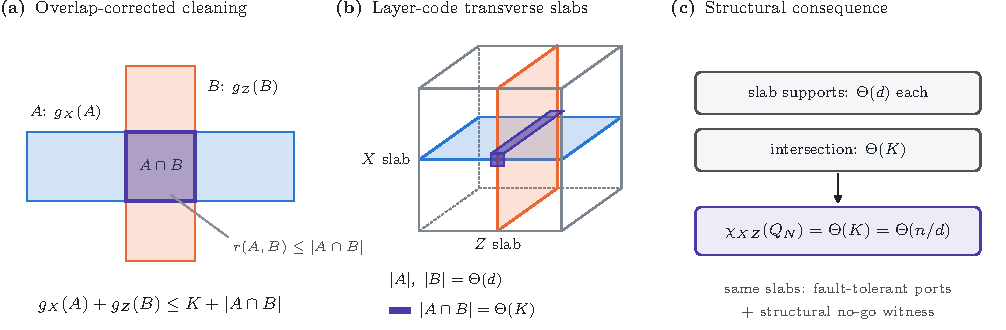
\includegraphics[width=0.95\textwidth]{symplectic_overlap_layer_ports.pdf}
\caption{Symplectic overlap of transverse logical ports.  \textbf{(a)} General CSS overlap-cleaning picture: if region $A$ supports $g_X(A)$ pure-$X$ logical classes and region $B$ supports $g_Z(B)$ pure-$Z$ logical classes, then the commutation they realize is constrained by the physical overlap, giving $g_X(A)+g_Z(B)\le K+|A\cap B|$.  In particular, any complete pure-$X$/pure-$Z$ polarization pair obeys $\chi_{XZ}(Q)\ge K$.  \textbf{(b)} In a layer code, the fixed $X$ and $Z$ slabs are both of size $\Theta(d)$ and intersect in a constant-cross-section tube of size $\Theta(K)$.  \textbf{(c)} The native slab pair is therefore simultaneously efficient in support size and overlap size: it attains $\chi_{XZ}(Q_N)=\Theta(K)=\Theta(n/d)$ while also serving as the local logical port structure used by the fault-tolerance architecture.}
\label{fig:symplectic-overlap}
\end{figure*}

Figure~\ref{fig:symplectic-overlap} summarizes the pairwise overlap-cleaning mechanism and the layer-code scaling it enforces; Theorem~\ref{thm:symplectic-crossbar} upgrades the same rank counting to the full two-polarization family.

Section~\ref{sec:supp-overlap} records extensions that are not needed by the architecture theorem: a sharp factor-of-two analog for arbitrary stabilizer codes, a symplectic rederivation of the Bravyi--Poulin--Terhal local-code tradeoff, the relation between $\chi_{XZ}$ and the price of a code, bipolar mobility--distance bounds and their exponent consequences, and the tile-code comparison.

\subsection{Repeated slabs, disjointness, and a shallow-unitary obstruction}
\label{sec:disjointness-obstruction}
We next use the stronger uniform-gap statement in a different way.  The same
bipolar mobility that saturates the crossbar bound also forces many
low-overlap representatives of every logical Pauli.  The result concerns a \emph{static} layer-code block and ordinary unitary circuits on its physical qubits; it does not constrain adaptive measurements, injected resources, ancillas, or code deformation used later in the architecture.  Figure~\ref{fig:slab-disjointness} summarizes the geometric mechanism: many disjoint same-orientation slab ports give a growing disjointness invariant, which in turn feeds directly into the Jochym-O'Connor--Kubica--Yoder shallow-circuit theorem.

For the single-qubit partition, let $\mathcal L$ be the nontrivial logical Pauli cosets.  Following Jochym-O'Connor, Kubica, and Yoder \cite{JochymDisjointness}, define
\begin{align}
 d_\downarrow&=\min_{G\in\mathcal L}d(G),&
 d_\uparrow&=\max_{G\in\mathcal L}d(G),
 \label{eq:minmax-distance}
\end{align}
where $d(G)$ is the minimum weight in the logical coset $G$.  A set of representatives of one $G$ is $c$-disjoint if each physical qubit lies in the support of at most $c$ representatives, and
\begin{align}
 \Delta_c(G)&=\frac{1}{c}\max\{|\mathcal A|:\mathcal A\subset G\text{ is $c$-disjoint}\},\nonumber\\
 \Delta&=\max_{c\ge1}\min_{G\in\mathcal L}\Delta_c(G).
 \label{eq:disjointness-def}
\end{align}

\begin{proposition}[Bipolar mobility lower-bounds disjointness]
\label{prop:mobility-disjointness}
Let an $[[n,K]]$ CSS code have $r_X$ pairwise-disjoint complete pure-$X$
ports and $r_Z$ pairwise-disjoint complete pure-$Z$ ports.  For the
single-qubit partition,
\begin{equation}
 \Delta(Q)\ge \frac12\min\{r_X,r_Z\}.
 \label{eq:mobility-disjointness}
\end{equation}
\end{proposition}

\begin{proof}
Put $r=\min\{r_X,r_Z\}$ and fix a nontrivial logical Pauli coset
$G=[X(u)Z(v)]$.  For $1\le i\le r$, choose a pure-$X$ representative
$X_i(u)$ in the $i$th $X$ port and a pure-$Z$ representative $Z_i(v)$ in
the $i$th $Z$ port, omitting a factor when its polarization is trivial, and
set $P_i=X_i(u)Z_i(v)\in G$.  Each physical qubit occurs in at most one of
the $X_i$ and at most one of the $Z_i$, hence in at most two of the $P_i$.
The $P_i$ are distinct: in the mixed case $P_i=P_j$ would force the pure-$X$
operator $X_iX_j$ to equal the pure-$Z$ operator $Z_iZ_j$ up to phase, and
therefore both to be identity, contradicting disjoint nonempty supports for
$i\ne j$; the pure cases are immediate.  Thus every nontrivial logical coset
has a $2$-disjoint set of size $r$, proving Eq.~\eqref{eq:mobility-disjointness}.
\end{proof}

\begin{theorem}[Layer-code disjointness and logical-weight symmetry]
\label{thm:layer-disjointness}
For the balanced good layer-code family considered in the architecture theorem (explicit realization, Theorem~\ref{thm:explicit-distance}), with the single-qubit partition,
\begin{equation}
 \Delta(Q_N)=\Theta(N),\qquad
 d_\downarrow=\Theta(N^2),\qquad
 d_\uparrow=\Theta(N^2).
 \label{eq:layer-disjointness-scaling}
\end{equation}
In particular $d_\uparrow/d_\downarrow=\Theta(1)$.
\end{theorem}
\begin{proof}
Corollary~\ref{cor:uniform-gap-slabs} gives $r_X,r_Z=\Theta(N)$ mutually
disjoint complete $X$- and $Z$-slab regions.  Proposition~\ref{prop:mobility-disjointness}
therefore gives $\Delta\ge\Omega(N)$.

For the reverse bound, Lemma~2 of Ref.~\cite{JochymDisjointness} proves $\Delta\le n_{\rm phys}/d_\uparrow$ for the single-qubit partition.  Every logical Pauli class has a representative obtained by multiplying one fixed $X$-slab representative and one fixed transverse $Z$-slab representative; bounded density and balanced block dimensions give weight $O(N^2)$.  Hence $d_\uparrow=O(N^2)$.  Since $d_\downarrow$ is the ordinary code distance and the family has $d_\downarrow=\Theta(N^2)$, necessarily $d_\uparrow\ge d_\downarrow=\Omega(N^2)$, so $d_\uparrow=\Theta(N^2)$.  With $n_{\rm phys}=\Theta(N^3)$, the published upper bound gives $\Delta=O(N)$, completing the proof.
\end{proof}

\begin{corollary}[Fixed-depth bounded-arity native unitaries are Clifford]
\label{cor:shallow-clifford-only}
Fix constants $q,h<\infty$.  There is $N_0(q,h)$ such that, for every $N\ge N_0(q,h)$, any code-preserving logical unitary implemented on one static layer-code block by a $q$-local physical circuit of depth $h$ lies in the logical Clifford group.  The physical gates need not be geometrically local.  In particular, sufficiently large blocks admit no within-block transversal logical $T$ gate, and more generally no bounded-arity constant-depth within-block non-Clifford logical unitary.
\end{corollary}
\begin{proof}
Theorem~9 of Jochym-O'Connor, Kubica, and Yoder states that a $q$-local depth-$h$ circuit can implement only a level-$M$ Clifford-hierarchy logical unitary whenever
\begin{equation}
 d_\uparrow q^{(2^M-1)h}<d_\downarrow\Delta^{M-1}
 \label{eq:jky-shallow-condition}
\end{equation}
\cite{JochymDisjointness}.  Set $M=2$.  Theorem~\ref{thm:layer-disjointness} gives
\begin{equation}
 \frac{d_\uparrow q^{3h}}{d_\downarrow\Delta}=O(N^{-1})\longrightarrow0.
\end{equation}
Thus Eq.~\eqref{eq:jky-shallow-condition} holds for all sufficiently large $N$, and the induced logical unitary lies in the second level, the Clifford group.  Transversal unitaries are the special case $q=1,h=1$.  By contrast, the Bravyi--K\"onig geometric-locality theorem permits third-level logical gates in three dimensions in general \cite{BravyiKoenig}; the stronger restriction here comes from the growing disjointness and does not assume geometric locality of the circuit.
\end{proof}

More generally, Proposition~\ref{prop:mobility-disjointness} and the same
Jochym-O'Connor--Kubica--Yoder criterion show that if
$m=\min\{r_X,r_Z\}$ and $d_\uparrow/d_\downarrow\le\rho$, then the sufficient
condition
\begin{equation}
 m>2\rho q^{3h}
 \label{eq:mobility-clifford-sufficient}
\end{equation}
forces every $q$-local depth-$h$ code-preserving logical unitary into the
Clifford group.  Thus growing two-polarization mobility simultaneously
supplies many measurement ports and strengthens the obstruction to static
shallow non-Clifford unitary gates.

\begin{figure*}[t]
\centering
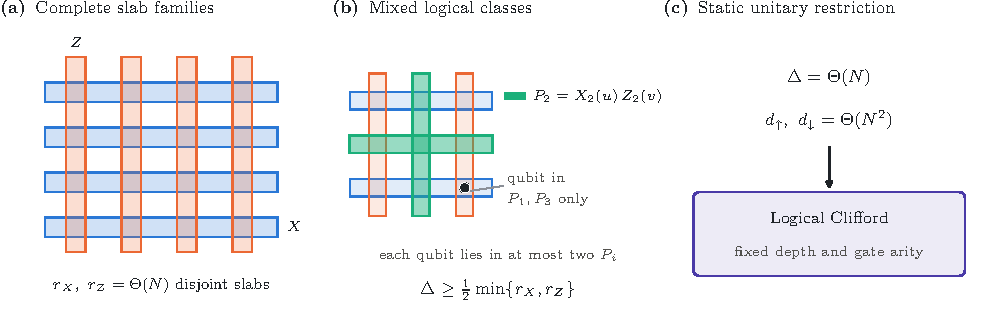
\includegraphics[width=0.94\textwidth]{slab_disjointness_clifford.pdf}
\caption{From uniform slab mobility to a Clifford-only shallow-unitary obstruction.  \textbf{(a)} Every height (for $X$) and every transverse position (for $Z$) supports every pure logical class, so balanced families provide $\Theta(N)$ mutually disjoint $X$-slab regions and $\Theta(N)$ mutually disjoint $Z$-slab regions.  \textbf{(b)} For a logical Pauli coset $G=[X(u)Z(v)]$, taking the $i$th pure-$X$ and pure-$Z$ representatives gives $P_i=X_i(u)Z_i(v)$.  Because any qubit can lie in at most one same-orientation slab of each type, the family $\{P_i\}$ is $2$-disjoint.  \textbf{(c)} Consequently $\Delta(Q_N)=\Theta(N)$ and $d_\uparrow,d_\downarrow=\Theta(N^2)$, so the Jochym-O'Connor--Kubica--Yoder criterion implies that any fixed-depth bounded-arity code-preserving unitary on a sufficiently large static layer-code block is logical Clifford.}
\label{fig:slab-disjointness}
\end{figure*}

Corollary~\ref{cor:uniform-gap-slabs} supplies the disjoint slab families used by this corollary.

\section{Slab certificate on complete check matrices}
\label{sec:certificate}

Theorem~\ref{thm:slab-resolved} and Proposition~\ref{prop:explicit-k} are
proved for arbitrary inputs.  The script \texttt{slab\_gluing\_certificate.py}
checks the same statements independently on complete finite codes, with
negative controls.  Every computation is exact GF(2) linear algebra on the
complete check matrices produced by \texttt{layer\_code\_explicit.py}; no check
is omitted and no boundary is treated as open.  (Its part A re-examines an
archived cell certificate of an earlier version; that material is in
Sec.~\ref{sec:archive}.)

\paragraph{Part B: complete codes.}
For seven input codes (Table~\ref{tab:slab-certificate}), including a code
with $K=7$, the surface code, and two random hypergraph-product codes, and
for spacings $s=2,3$ where feasible, the script builds the complete explicit
realization and verifies: all checks commute; the wall system of every
crossing line is solved; $n-\#X-\#Z$ equals $n_{\rm in}-m_X-m_Z$ and the
relation spaces have the input dimensions (the two steps of
Proposition~\ref{prop:explicit-k}); and $k=K$.  The same inputs built in the
single-chart transcription give valid CSS codes (a plain union of sheets is a
cell complex), but with $k\neq K$ in every case.

\paragraph{Part C: gluing forms.}
The prefix operator is written as a sum of binary variables, one per data
string ($x_q$) and one per backbone segment ($p^{(j)}_t$), each a fixed edge
set.  For every stabilizer the script computes the linear form in these
variables given by its overlap parity and compares the set of nonzero forms
with the first/middle/last relations of Eq.~\eqref{eq:local-prefix-parity}.
In the explicit realization the forms are exactly these relations, one face
per incidence, at every height $z_0$ and, dually, at every column $x_0$
(Theorem~\ref{thm:slab-resolved}(1)).  In the single-chart transcription every
middle incidence produces the two forms $x_{q_t}+p_{t-1}$ and $x_{q_t}+p_t$,
i.e.\ the all-equal relation.

\paragraph{Part D: exhaustive words, negative controls, and logical checks.}
For a single check of weight $2\le k\le6$ every incidence word and every
backbone assignment ($2^{2k-1}$ assignments) is tried.  In the explicit
realization the zero-syndrome assignments are exactly the $2^{k-1}$ even words
with their prefix backbones; every other assignment, including odd words and
every single-segment flip, violates at least one stabilizer at the
offending incidence.  In the single-chart transcription only the constant
words survive.  For every input code, every basis vector of $\ker H_Z$
($\ker H_X$), and every height (column), the slab operator commutes with every
stabilizer; stabilizer inputs map to stabilizers; the pairing with the dual
slabs equals the input pairing; and its rank is $K$.

\paragraph{Part E: point defects.}
Walls close exactly when the input checks commute.  For five pairs of one
$X$ and one $Z$ check with overlaps $2,1,3,4,3$ (built without the CSS
requirement), the wall system is inconsistent for every odd overlap and
solvable for every even one, as Lemma~\ref{lem:explicit-commute} states.

\begin{table*}[t]
\caption{Complete-code certificate (\texttt{slab\_cert\_B\_complete\_codes.csv},
\texttt{slab\_cert\_C\_forms.csv}).  ``Forms'' counts heights (columns) at
which the nonzero gluing forms are exactly the prefix relations; ``ops''
counts slab operators, over all basis inputs and positions, that commute with
every stabilizer; ``rank'' is the rank of the $X$/$Z$ slab pairing.  The last
two columns are the single-chart transcription of the same input.}
\label{tab:slab-certificate}
\centering
\scriptsize
\setlength{\tabcolsep}{3.5pt}
\begin{tabular}{@{}lrrrrrrrrrr|rr@{}}
\toprule
Input & $s$ & $n$ & $K$ & $k$ & anticomm. & $X$ forms & $Z$ forms & $X$ ops & $Z$ ops & rank & $k$ (1-chart) & $X$ ops (1-chart) \\
\midrule
$[[4,2,2]]$ & 2 & 224 & 2 & 2 & 0 & 4/4 & 5/5 & 12/12 & 15/15 & 2 & 4 & 0/12 \\
$[[4,2,2]]$ & 3 & 504 & 2 & 2 & 0 & 6/6 & 7/7 & 18/18 & 21/21 & 2 & 4 & 0/18 \\
$[[6,4,2]]$ & 2 & 352 & 4 & 4 & 0 & 4/4 & 5/5 & 20/20 & 25/25 & 4 & 6 & 0/20 \\
$[[6,4,2]]$ & 3 & 792 & 4 & 4 & 0 & 6/6 & 7/7 & 30/30 & 35/35 & 4 & 6 & 0/30 \\
Steane $[[7,1,3]]$ & 2 & 1792 & 1 & 1 & 0 & 8/8 & 9/9 & 32/32 & 36/36 & 1 & 10 & 0/32 \\
Steane $[[7,1,3]]$ & 3 & 4032 & 1 & 1 & 0 & 12/12 & 13/13 & 48/48 & 52/52 & 1 & 10 & 0/48 \\
Hamming $[[15,7,3]]$ & 2 & 6600 & 7 & 7 & 0 & 10/10 & 11/11 & 110/110 & 121/121 & 7 & 29 & 0/110 \\
surface $[[13,1,3]]$ & 2 & 10314 & 1 & 1 & 0 & 14/14 & 15/15 & 98/98 & 105/105 & 1 & 15 & 0/98 \\
random HGP 1 & 2 & 10936 & 2 & 2 & 0 & 14/14 & 15/15 & 98/98 & 120/120 & 2 & 20 & 0/98 \\
random HGP 2 & 2 & 10512 & 2 & 2 & 0 & 14/14 & 15/15 & 98/98 & 120/120 & 2 & 18 & 0/98 \\
\bottomrule
\end{tabular}
\end{table*}

\paragraph{Rank criterion.}
For any finite CSS code the following criterion decides whether a region
$S$ supports every pure logical class; the certificate does not need it,
because it constructs the representatives, but it remains a convenient
independent test.  With $\rho_X=\rank H_X$, $\rho_Z=\rank H_Z$ and $\overline S$ the
complement, every pure-$X$ class has a representative in $S$ if and only if
\begin{equation}
 |S|-\rank(H_Z|_S)-\rho_X+\rank(H_X|_{\overline S})=k,
 \label{eq:slab-rank-x}
\end{equation}
and dually
\begin{equation}
 |S|-\rank(H_X|_S)-\rho_Z+\rank(H_Z|_{\overline S})=k.
 \label{eq:slab-rank-z}
\end{equation}
The left side of Eq.~\eqref{eq:slab-rank-x} is the dimension of the image of
$\ker H_Z\cap\mathbb F_2^S$ in $\ker H_Z/\operatorname{row}H_X$.


\section{Grid expansion and local gauging}\label{sec:gauging}
% Requires amsmath, amssymb, amsthm.

\paragraph{The idea in plain terms.}
Gauging measures a logical $\overline P=X(D)$ through many local vertex
checks on an ancilla grid whose product is $\overline P$.  The added qubits
may create short logical operators, and the whole section controls one
quantity that rules them out.  An $X$ logical of the deformed code can only
place its ancilla part on a \emph{wall}, the set $\delta T$ of edges leaving
some vertex set $T$.  Multiplying by the vertex checks in $T$ trades that wall
for $X$ on the data qubits attached in $T$, which turns the operator into a
logical of the original code.  This trade never helps a short operator if
every wall has at least as many edges as the ports it separates, which is the
relative expansion $\beta\ge1$ (Proposition~\ref{prop:gauging-distance}).
Conversely, a small wall between the ports of two blocks is itself a short
logical (Proposition~\ref{prop:cut-obstruction}): a thin interface fails.
The slab theorem puts the ports in one plane, and in a three-dimensional box
as thick as it is wide every wall is a surface whose area grows with the
number of ports it separates, so $\beta$ is a constant
(Lemmas~\ref{lem:rectangle-cheeger} and~\ref{lem:thickening}); a constant
number of ancillas per edge then gives $\beta\ge1$
(Corollary~\ref{cor:edge-multiplicity}).

\paragraph{Notation for ports and relative expansion.}
Let $C$ be a CSS stabilizer code, let $\overline P=X(D)$ be a nontrivial
$X$-type logical representative with data support $D$, and let
$G=(W,E)$ be a connected graph.  A port map is an injection
$f:D\hookrightarrow W$, and we write $U=f(D)$.  Vertices in $W\setminus U$
are called dummy vertices.  For $T\subseteq W$, let $\delta T$ be the set of
edges with exactly one endpoint in $T$.  For $U\subseteq W$ define
\begin{equation}
 \beta(G,U)=
 \min_{\substack{T\subseteq W\\
       \min\{|T\cap U|,|U\setminus T|\}>0}}
 \frac{|\delta T|}{\min\{|T\cap U|,|U\setminus T|\}}.
 \label{eq:relative-expansion}
\end{equation}
We use the convention $\beta(G,U)=+\infty$ when $|U|\leq 1$.

\paragraph{Gauged generators.}
For every vertex $u$, let
\begin{align}
 A_u&=X_{f^{-1}(u)}\prod_{e\ni u}X_e, && u\in U,\\
 A_u&=\prod_{e\ni u}X_e, && u\notin U.
\end{align}
Use $B_c=\prod_{e\in c}Z_e$ for a cycle-space generating set, retain the $X$ checks of $C$, and replace a $Z$ check $s$ by $\widetilde s=s\prod_{e\in\mu_s}Z_e$, where $\partial\mu_s=f(\operatorname{supp}(s)\cap D)$. This boundary is even because $s$ commutes with the measured logical. Connectedness of $G$ supplies such $\mu_s$. These are the usual gauging generators of Ref.~\cite{WilliamsonYoderGauging}.

\paragraph{Deformed-code distance.}
The following formulation separates data qubits from graph vertices and
also records the two degenerate cases used below.

\begin{proposition}[Distance under gauging]
\label{prop:gauging-distance}
Let $C$ have CSS distances $d_X,d_Z$.  Gauge the representative
$\overline P=X(D)$ using a connected graph $G=(W,E)$ and an injective port
map $f:D\hookrightarrow W$.  Put $U=f(D)$ and
$\beta=\beta(G,U)$.  The deformed code is CSS and satisfies
\begin{equation}
 d_X(\widetilde C)\geq \min\{1,\beta\}d_X,
 \qquad
 d_Z(\widetilde C)\geq d_Z.
 \label{eq:gauging-distance}
\end{equation}
Dummy vertices require no separate hypothesis: $\beta$ in
\eqref{eq:gauging-distance} is computed on the final graph,
including all dummy vertices.

If $D=\varnothing$, no logical is gauged.  The graph ancilla generated by
all vertex stars and by a basis of the cycle space is a stabilizer state, so
the resulting code is $C$ tensored with that state and has the same logical
distances as $C$.

If $C=C_1\otimes C_2$ and the measured Pauli is a product of one logical
from each factor, the same conclusion holds with $d_X$ and $d_Z$ replaced
by the minima of the corresponding distances of the two blocks.
The statement with $X$ and $Z$ exchanged also holds.
\end{proposition}

With the Cheeger constant $h(G)$ in place of $\beta$, this is Lemma~2 (space
fault-distance) in the Methods of the published version of
Ref.~\cite{WilliamsonYoderGauging}; the relative form below follows the same
cut argument.

\begin{proof}
All displayed generators of the gauged code are of pure $X$ or pure $Z$
type, so the code is CSS.  Let
$L'=X(A)X(F)$ be an $X$-type logical of the deformed code, where $A$ is a
set of data qubits and $F\subseteq E$.  Commutation with every cycle
generator says that $F$ is orthogonal to the cycle space.  Because $G$ is
connected, the orthogonal complement of its cycle space is its cut space;
hence $F=\delta T$ for some $T\subseteq W$.  Multiplication by
$\prod_{u\in T}A_u$ removes the edge support and gives
\begin{equation}
 L''=X\bigl(A\mathbin\triangle f^{-1}(T\cap U)\bigr).
\end{equation}
This operator commutes with every check of $C$.  If $L'$ is nontrivial,
neither $L''$ nor $L''\overline P$ is an $X$ stabilizer of $C$; otherwise
$L'$ would be generated by the deformed stabilizers.  Consequently both
have weight at least $d_X$.  Choose between $T$ and $W\setminus T$ so that
the chosen port side has cardinality
$m=\min\{|T\cap U|,|U\setminus T|\}$.  The corresponding one of $L''$ and
$L''\overline P$ has support contained in the symmetric difference of
$A$ with a set of $m$ data qubits.  Put $b_0=\min\{1,\beta\}$. For every cut, including a cut with $m=0$, $|\delta T|\geq b_0m$. Therefore
\begin{align}
 |L'|&=|A|+|\delta T| \\
 &\geq |A|+b_0m \\
 &\geq \min\{1,\beta\}(|A|+m) \\
 &\geq \min\{1,\beta\}d_X.
\end{align}

Now let $L'=Z(B)Z(F)$ be a $Z$-type logical.  The unchanged $X$ checks imply
that $Z(B)$ lies in the normalizer of $C$.  Commutation with every vertex
operator gives
\begin{equation}
 \partial F=f(B\cap D),
\end{equation}
and hence $|B\cap D|=|\partial F|=0\pmod 2$.  Thus $Z(B)$ commutes with
$\overline P$.  If $Z(B)$ is a stabilizer of $C$, multiplying $L'$ by the
corresponding deformed $Z$ checks leaves a pure edge cycle, which is a
product of the chosen cycle generators; in that case $L'$ is trivial.
Otherwise $|L'|\geq |B|\geq d_Z$.

For $D=\varnothing$, the graph ancilla has $|W|-1$ independent vertex
stars and $|E|-|W|+1$ independent cycle generators, for a total of $|E|$
independent stabilizers on $|E|$ edge qubits.  It therefore encodes no
qubit.  The product-code claim follows from the same proof because a
nontrivial logical on $C_1\otimes C_2$ has weight at least the minimum of
the two component distances.
\end{proof}


\paragraph{Why added measurement layers can lose distance.}
Proposition~\ref{prop:gauging-distance} is a lower bound.  The converse below
shows that the relative expansion is the quantity that must be controlled, and
it makes precise the concern that attaching an additional measurement layer to
a code can lower its fault distance.  When the ports of two independent
logical factors are separated by a small cut of the ancilla graph, the
deformed code acquires a correspondingly short logical operator.

\begin{proposition}[Cut obstruction]
\label{prop:cut-obstruction}
In the setting of Proposition~\ref{prop:gauging-distance}, suppose that
$D=D_1\sqcup D_2$, that $X(D_1)$ commutes with every check of $C$, and that
$X(D_1)\notin\langle S_X(C),\overline P\rangle$.  If $T\subseteq W$ satisfies
$T\cap U=f(D_1)$, then $X(\delta T)$ is a nontrivial $X$-type logical operator
of the deformed code and represents the same class as $X(D_1)$.  Consequently
\begin{equation}
 d_X(\widetilde C)\leq
 \min\bigl\{|\delta T|:\ T\subseteq W,\ T\cap U=f(D_1)\bigr\},
 \label{eq:cut-obstruction}
\end{equation}
the size of a minimum edge cut of $G$ separating $f(D_1)$ from $f(D_2)$.
\end{proposition}

\begin{proof}
Because $T\cap U=f(D_1)$, the product of the vertex operators in $T$ is
$\prod_{u\in T}A_u=X(D_1)X(\delta T)$.  The operator $X(D_1)$ has no edge
support and commutes with every check of $C$.  It therefore commutes with
every cycle generator $B_c$ and with every deformed check $\widetilde s$,
whose data part is $s$.  Thus $X(D_1)$ lies in the deformed normalizer, and
so does $X(\delta T)=X(D_1)\prod_{u\in T}A_u$, which represents the same
class.  Suppose this class were trivial.  Then $X(D_1)=\sigma\prod_{u\in
T'}A_u$ for some $\sigma\in S_X(C)$ and $T'\subseteq W$.  The edge support of
the right side is $\delta T'$, which must vanish, so connectedness gives
$T'\in\{\varnothing,W\}$.  Since $\prod_{u\in W}A_u=\overline P$, this
places $X(D_1)$ in $\langle S_X(C),\overline P\rangle$, contrary to
assumption.
\end{proof}

\begin{corollary}[Thin interfaces for joint measurements]
\label{cor:thin-interface}
Let $C=C_a\otimes C_b$ and gauge $\overline P=\overline X_a\overline X_b$,
where $\overline X_a=X(D_a)$ and $\overline X_b=X(D_b)$ are nontrivial
logical operators of the two blocks.  Then $d_X(\widetilde C)$ is at most the
minimum number of ancilla edges whose removal separates $f(D_a)$ from
$f(D_b)$ in $G$, however large the distances of $C_a$ and $C_b$ are.
\end{corollary}

\begin{proof}
Apply Proposition~\ref{prop:cut-obstruction} with $D_1=D_a$.  The operator
$X(D_a)$ commutes with every check of $C_a\otimes C_b$.  It is not in
$S_X(C)$, because its restriction to block $a$ is the nontrivial
$\overline X_a$.  It is not in the coset $S_X(C)\overline P$, because every
element of that coset restricts to $\overline X_b$ times a stabilizer on block
$b$, whereas $X(D_a)$ acts trivially there.
\end{proof}

\paragraph{Geometric consequence for layer codes.}
For a geometrically local ancilla of bounded density, every path joining the
two port sets crosses any surface separating the two blocks.  If the ancilla
joins two adjacent blocks only through a layer of thickness $h$ and width $w$,
Corollary~\ref{cor:thin-interface} therefore gives $d_X(\widetilde C)=O(hw)$.
For the balanced layer codes, a block has linear size $\Theta(N)$ and
$d=\Theta(N^2)$ is of the same order as the area of one block face.  This is
generic for distance-optimal three-dimensional codes, since
$d=O(L^2)$ for any local stabilizer code of linear size $L$ in three
dimensions \cite{BravyiTerhal2009}.  A measurement layer of bounded thickness thus loses
a factor $\Theta(N)$ of distance in every joint measurement, and a joint
measurement that keeps distance $\Theta(d)$ must cross a constant fraction of
the full $\Theta(N^2)$ interface between the blocks.  Joint measurements are
unavoidable in the gate set of Sec.~\ref{sec:gates} (CNOT and phase
teleportation) and in resource transfer (Sec.~\ref{sec:ft}).  The grid box of
Theorem~\ref{thm:local-gauging} spans both blocks, so its separating cuts have
size $\Omega(N^2)$; this is the content of
Corollary~\ref{cor:cubic-box-relative-expansion}.  Corollary~\ref{cor:thin-interface} does not
exclude thin layers for measuring a single logical inside one block, but the
construction does not rely on that case.

\paragraph{Explicit check.}
Table~\ref{tab:interface-check} applies
Propositions~\ref{prop:gauging-distance} and~\ref{prop:cut-obstruction} to two
periodic three-dimensional toric codes of linear size $L$.  Their $X$ logical
is a membrane of weight $L^2$ supported in one plane, a small stand-in for a
slab representative.  The joint logical $\overline X_a\overline X_b$ is
gauged with a $2L\times L\times H$ cubic-grid ancilla whose plane number
$\lfloor H/2\rfloor$ (counting the $H$ planes from zero) contains both membranes.  For each instance the script
\texttt{measurement\_interface\_check.py} constructs the deformed code, checks
$H_XH_Z^{\mathsf T}=0$, and verifies over GF(2) that $X(\delta T)$ is a
nontrivial deformed logical equivalent to $\overline X_a$, while
$\overline X_a\overline X_b$ is a deformed stabilizer.  The lower end of each
bracket is Proposition~\ref{prop:gauging-distance} with
$\beta\geq m\min\{1,H/(2L)\}$ (Lemmas~\ref{lem:rectangle-cheeger}
and~\ref{lem:thickening} with one port plane).  A single added sheet ($H=1$)
leaves a deformed distance between $L/2$ and $L$, whereas the thick box keeps
at least $L^2/2$.  With two ancillas per grid edge
(Corollary~\ref{cor:edge-multiplicity}) the thick box keeps exactly $L^2$.
For $L=3$ an exact CP-SAT computation closes every bracket at its upper end:
the deformed distances are $3$, $6$ and $9$ for $H=1,2,3$
(Table~\ref{tab:slice-check}).

\begin{table}[t]
\caption{Deformed $X$ distance for the joint measurement
$\overline X_a\overline X_b$ of two periodic three-dimensional toric codes,
bracketed between the relative-expansion lower bound and the explicit cut
logical (or $\overline X_a$).  Here $H$ is the ancilla thickness and $m$ the
number of ancilla qubits per grid edge.  Source:
\texttt{measurement\_interface\_check.csv}.}
\label{tab:interface-check}
\begin{ruledtabular}
\begin{tabular}{cccccc}
$L$ & $d_X$ & $H=1$ & $H=2$ & $H=L$ & $H=L$, $m=2$\\
\colrule
3 & 9  & $[2,3]$ & $[3,6]$  & $[5,9]$   & 9\\
4 & 16 & $[2,4]$ & $[4,8]$  & $[8,16]$  & 16\\
5 & 25 & $[3,5]$ & $[5,10]$ & $[13,25]$ & 25\\
6 & 36 & $[3,6]$ & $[6,12]$ & $[18,36]$ & 36\\
\end{tabular}
\end{ruledtabular}
\end{table}

\paragraph{Full distance at constant ancilla multiplicity.}
Proposition~\ref{prop:gauging-distance} loses the factor $\min\{1,\beta\}$
only when $\beta<1$.  Because the grid relative expansion is a positive
constant, a constant number of parallel ancillas per edge removes this loss.

\begin{corollary}[Edge multiplicity restores the full distance]
\label{cor:edge-multiplicity}
Let $G^{(m)}$ be obtained from the connected graph $G$ by replacing every
edge with $m$ parallel edges, each carrying its own ancilla qubit.  Then
$\beta(G^{(m)},U)=m\,\beta(G,U)$.  Gauge $\overline P$ on $G^{(m)}$ with
vertex operators acting on all parallel copies, pairing paths on one
designated copy of each edge, and cycle generators consisting of the chosen
cycle generators of $G$ on the designated copies together with the
weight-two bundle cycles $Z_eZ_{e'}$ of parallel edges.  If
$m\geq1/\beta(G,U)$, then
\begin{equation}
 d_X(\widetilde C)\geq d_X,\qquad d_Z(\widetilde C)\geq d_Z.
 \label{eq:full-distance}
\end{equation}
The same holds in the $X\leftrightarrow Z$ dual convention, and the factor
$\min\{1,\beta\}$ in Lemmas~\ref{lem:bare-port-quotient}
and~\ref{lem:encoded-port-quotient} is likewise replaced by
$\min\{1,m\beta\}$.
\end{corollary}

\begin{proof}
Every cut of $G^{(m)}$ consists of all $m$ copies of the edges of the
corresponding cut of $G$, so $|\delta^{(m)}T|=m|\delta T|$ for all
$T\subseteq W$, and the relative expansion scales by $m$.  The displayed
generators span the cycle space of $G^{(m)}$: replacing every copy of an edge
by its designated copy using bundle cycles leaves an even-degree edge set of
$G$.  The proof of Proposition~\ref{prop:gauging-distance} uses only
connectedness and the fact that the cut space is the orthogonal complement of
the cycle space.  Both hold for multigraphs, since an edge set orthogonal to
every bundle cycle contains all or none of the copies of each edge.  Hence
$d_X(\widetilde C)\geq\min\{1,m\beta\}d_X=d_X$.  The $Z$ bound is unchanged,
and the two quotient lemmas use the same cut estimate.
\end{proof}

\paragraph{Raw-injection intuition.}
\label{par:raw-injection-intuition}
Before stating the bare-port quotient lemma, record the intended picture
(Fig.~\ref{fig:raw-injection}): appending an unchecked physical resource qubit creates a
weight-one logical class, but that class is precisely the \emph{intentional traveling resource}.
Every spectator logical of the data block remains at distance $\Omega(d)$ after gauging, by the
quotient statement below; subsequent encoded-courier stages never reintroduce a bare port.
\begin{figure}[t]
\centering
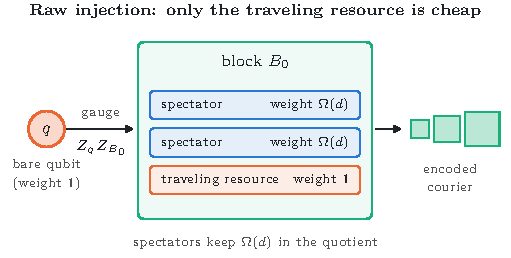
\includegraphics[width=\columnwidth]{raw_injection_intuition.pdf}
\caption{Bare-port intuition.  Raw injection creates a weight-one traveling-resource class, while all spectator logicals remain $\Omega(d)$ in the quotient (Lemma~\ref{lem:bare-port-quotient}).  Only encoded courier stages appear downstream.}
\label{fig:raw-injection}
\end{figure}

\paragraph{A bare injection port.}
The distance-one product code obtained by appending an unchecked qubit
cannot be inserted directly into Proposition~\ref{prop:gauging-distance}
to obtain a block-distance bound.  The required statement is a relative
distance assertion.

\begin{lemma}[Bare-port quotient distance]
\label{lem:bare-port-quotient}
Let $C_b$ be a CSS block with $X$ and $Z$ distances at least $d$, append an
unchecked qubit $q$, and gauge
$M=\overline Z Z_q$ using the $X\leftrightarrow Z$ dual convention on a
connected graph with relative expansion $\beta$.  In the deformed logical
Pauli group, every class outside the subgroup generated by $[Z_q]$ has
minimum weight at least $\min\{1,\beta\}d$.  The exceptional class has the
weight-one representative $Z_q$, and the new stabilizer relation
$M=1$ identifies its action with that of $\overline Z$ on the block.
The analogous statement holds with $X$ and $Z$ exchanged.
\end{lemma}

\begin{proof}
In this dual convention the $Z$-type logicals admit the cut-space reduction. Multiplying by the Gauss operators removes the edge support and produces a $Z$ normalizer on $C_b\otimes q$, with the two complementary reductions differing by $M$. For a class outside $\langle[Z_q]\rangle$, the block part of each reduction is outside $\langle S_Z(C_b),\overline Z\rangle$: otherwise the reduced operator, and hence the original class, is generated by $M$, $Z_q$, and stabilizers. Each block part consequently has weight at least $d$. Choosing the smaller port side and using the preceding finite $b_0=\min\{1,\beta\}$ estimate proves the $b_0d$ bound for these $Z$ classes.

For an $X$-type logical, the cycle-space reduction restricts its data part to $X(B)X_q^b$, where $X(B)$ is a block normalizer. Commutation with the product of the dual Gauss operators gives $b=\langle X(B),\overline Z\rangle$. If $X(B)$ is a block stabilizer, then $b=0$ and the remaining edge cycle is trivial modulo the deformed checks. Thus every nontrivial $X$ logical has a nontrivial block restriction and weight at least $d$.

The code is CSS, so any Pauli normalizer factors as $L=L_XL_Z$, with both pure components separately in its normalizer. If $[L]\notin\langle[Z_q]\rangle$, either $[L_X]$ is nontrivial or $[L_Z]\notin\langle[Z_q]\rangle$. The corresponding component has weight at least $b_0d$, and $\mathrm{wt}(L)=|\operatorname{supp}(L_X)\cup\operatorname{supp}(L_Z)|$ is at least that component's weight. This proves the mixed-Pauli assertion too.

Finally $Z_q$ commutes with every deformed generator. It is nontrivial: choose a block $X$ logical anticommuting with $\overline Z$, append $X_q$, and extend it over edges using connectedness to solve the even boundary constraint. The resulting deformed normalizer anticommutes with $Z_q$. The stabilizer $M$ gives $[Z_q]=[\overline Z]$.
\end{proof}

\paragraph{Encoded ports of unequal distance.}
Resource transfer joins a small courier block to a larger block
(Sec.~\ref{sec:ft}).  Proposition~\ref{prop:gauging-distance} then gives only
the smaller distance.  The quotient statement below shows that the smaller
block exposes only its own logical classes; every other logical class keeps
the distance of the larger block.  Lemma~\ref{lem:bare-port-quotient} is the
special case in which $C_1$ is a single unchecked qubit.

\begin{lemma}[Encoded-port quotient distance]
\label{lem:encoded-port-quotient}
Let $C_1$ and $C_2$ be CSS codes, where $C_2$ has $X$ and $Z$ distances at
least $d_2$ and $C_1$ is arbitrary.  Let $\overline Z_1=Z(D_1)$ and
$\overline Z_2=Z(D_2)$ be nontrivial logical representatives, and gauge
$M=\overline Z_1\overline Z_2$ on $C_1\otimes C_2$ in the $X\leftrightarrow Z$
dual convention, using a connected graph with relative expansion $\beta$ with
respect to $U=f(D_1\sqcup D_2)$.  Let $\mathcal Q_1$ be the group of deformed
logical classes obtained from logical operators of $C_1$ that commute with
$\overline Z_1$; an $X$-type operator $X(B_1)$ is completed by edge operators
$X(F)$ with $\partial F=f(B_1\cap D_1)$.  Then
$[\overline Z_2]=[\overline Z_1]\in\mathcal Q_1$, and every deformed logical
class outside $\mathcal Q_1$ has minimum weight at least $\min\{1,\beta\}d_2$.
\end{lemma}

\begin{proof}
In the dual convention the vertex operators are
$A_u=Z_{f^{-1}(u)}\prod_{e\ni u}Z_e$ (without the data factor at dummy
vertices), the cycle generators are $X$-type, the $Z$ checks of
$C_1\otimes C_2$ are retained, and each $X$ check $s$ is replaced by
$\widetilde s=s\prod_{e\in\mu_s}X_e$.  The relation $\prod_uA_u=M$ gives
$[\overline Z_2]=[\overline Z_1]$.

\emph{$X$-type classes.}  Let $L'=X(B)X(F)$ be a deformed logical operator
and write $X(B)=X(B_1)X(B_2)$ by block.  Commutation with the vertex
operators gives $\partial F=f(B\cap D)$, so $X(B)$ commutes with $M$, and
commutation with the retained $Z$ checks shows that $X(B)$ commutes with
every check of $C_1\otimes C_2$.  Two deformed operators with the same data
part differ by an edge cycle, and data parts that differ by an $X$ stabilizer
$\sigma$ of $C_1\otimes C_2$ are related by the deformed check
$\widetilde\sigma$ up to a cycle.  Hence $[L']$ depends only on the logical
class of $X(B)$.  If $X(B_2)$ is a stabilizer of $C_2$, then $X(B_1)$
commutes with $\overline Z_1$ and $[L']\in\mathcal Q_1$.  Otherwise $X(B_2)$
is a nontrivial logical operator of $C_2$, and $|L'|\geq|B_2|\geq d_2$.

\emph{$Z$-type classes.}  Let $L'=Z(A)Z(F)$.  Commutation with the $X$-type
cycle generators makes $F$ orthogonal to the cycle space, so $F=\delta T$ for
some $T\subseteq W$.  Multiplying by $\prod_{u\in T}A_u$ or by
$\prod_{u\in W\setminus T}A_u$ gives two data reductions, $L''$ and $L''M$.
Both are $Z$-type operators commuting with every check of $C_1\otimes C_2$,
and both represent $[L']$.  If the $C_2$ part of $L''$ lies in
$\langle S_Z(C_2),\overline Z_2\rangle$, then $L''$ is a $Z$-type operator on
$C_1$ times a stabilizer times a power of $\overline Z_2$.  A $Z$-type
operator on $C_1$ commutes with $\overline Z_1$ and needs no edge completion,
so $[L']\in\mathcal Q_1$.  Otherwise the $C_2$ parts of $L''$ and of $L''M$
are both nontrivial logical operators of $C_2$, so both reductions have weight
at least $d_2$.  The reduction associated with the smaller port side is
supported in the symmetric difference of $A$ with a set of
$m=\min\{|T\cap U|,|U\setminus T|\}$ data qubits.  As in
Proposition~\ref{prop:gauging-distance}, with $b_0=\min\{1,\beta\}$,
\begin{equation*}
 |L'|=|A|+|\delta T|\geq|A|+b_0m\geq b_0(|A|+m)\geq b_0d_2.
\end{equation*}

\emph{Mixed classes.}  The deformed code is CSS, so every normalizer element
factors as $L=L_XL_Z$ with both factors in the normalizer.  The group
$\mathcal Q_1$ is generated by pure-type classes, because the $X$ part of a
logical operator of $C_1$ commuting with $\overline Z_1$ also commutes with
$\overline Z_1$.  A class outside $\mathcal Q_1$ therefore has a pure
component outside $\mathcal Q_1$, and the bound for that component applies to
the whole operator.
\end{proof}

\paragraph{Cheeger bound for a rectangular grid.}
\begin{lemma}
\label{lem:rectangle-cheeger}
Let $G_0=[a]\mathbin\square[b]$ be the rectangular grid with $a\leq b$.
For every $S\subseteq V(G_0)$ with $|S|\leq ab/2$,
\begin{equation}
 |\delta S|\geq \frac{|S|}{b}.
\end{equation}
In particular, $h(G_0)\geq 1/b$.
\end{lemma}

\begin{proof}
Call a row or column full, empty, or mixed according to its intersection
with $S$.  If a full and an empty row both exist, every column contains a
boundary edge, so $|\delta S|\geq b\geq |S|/b$.  If no row is full, every
row meeting $S$ contains a boundary edge, and at least $|S|/b$ rows meet
$S$.  In the remaining case some row is full and no row is empty.  Every
column meets $S$, while at most $|S|/a\leq b/2$ columns are full.  Hence at
least $b/2$ columns are mixed.  Since
$b/2\geq |S|/a\geq |S|/b$, the result follows.
\end{proof}

\paragraph{Thickening relative to several layers.}
\begin{lemma}[Thickening]
\label{lem:thickening}
Let $G=G_0\mathbin\square P_\ell$, where $G_0$ is connected and $P_\ell$
is a path on $\ell$ vertices.  If $U\subseteq V(G)$ is contained in the
union of at most $t$ layers, then
\begin{equation}
 \beta(G,U)\geq \frac{\min\{1,\ell h(G_0)\}}{2t}.
 \label{eq:thickening}
\end{equation}
If $U$ is contained in a single layer, the factor $2$ can be omitted.
\end{lemma}

\begin{proof}
Fix a set $T\subseteq V(G)$ occurring in
\eqref{eq:relative-expansion}.  Let $T_j\subseteq V(G_0)$ be its
intersection with layer $j$.  Put
$J=\{j:U\text{ meets layer }j\}$, so $|J|\leq t$, choose $j_0\in J$, and
define
\begin{equation}
 m=\max_j|T_j\mathbin\triangle T_{j_0}|,
 \qquad
 \mu=\min\{|T_{j_0}|,|V(G_0)\setminus T_{j_0}|\}.
\end{equation}
For each vertex of $T_j\mathbin\triangle T_{j_0}$, the vertical column
joining layers $j$ and $j_0$ contains an edge of $\delta T$.  These columns
are distinct, so the vertical part of the boundary has size at least $m$.
For every $j$,
\begin{equation}
 \min\{|T_j|,|V(G_0)\setminus T_j|\}
 \geq \max\{0,\mu-m\}.
\end{equation}
Summing the Cheeger bound over all layers shows that the horizontal part
has size at least
$\ell h(G_0)\max\{0,\mu-m\}$.  The horizontal and vertical boundary edges
are disjoint.  With $c=\min\{1,\ell h(G_0)\}$,
\begin{equation}
 |\delta T|
 \geq m+c\max\{0,\mu-m\}
 \geq c\max\{\mu,m\}.
 \label{eq:thickening-boundary}
\end{equation}
On the other hand,
\begin{align}
 |T\cap U|&\leq |J|\bigl(|T_{j_0}|+m\bigr),\\
 |U\setminus T|&\leq |J|\bigl(|V(G_0)\setminus T_{j_0}|+m\bigr).
\end{align}
Therefore
\begin{equation}
 \min\{|T\cap U|,|U\setminus T|\}
 \leq |J|(\mu+m)
 \leq 2t\max\{\mu,m\}.
\end{equation}
Combining this with \eqref{eq:thickening-boundary} proves
\eqref{eq:thickening}.  If $t=1$, choose $j_0$ to be the unique
occupied layer.  Then the denominator is at most $\mu$, so the factor $2$
is unnecessary.
\end{proof}

\paragraph{Cubic boxes.}
\begin{corollary}
\label{cor:cubic-box-relative-expansion}
Let $B=[a_1]\times[a_2]\times[a_3]$ be a cubic-lattice box, let
$a_{\max}=\max_i a_i$ and $a_{\min}=\min_i a_i$, and let $\Gamma_B$ be its
grid graph.  If $U$ is contained in at most $t$ coordinate planes
perpendicular to one axis, then
\begin{equation}
 \beta(\Gamma_B,U)\geq \frac{a_{\min}}{2t a_{\max}}.
\end{equation}
\end{corollary}

\begin{proof}
Take $G_0$ to be the rectangular cross-section parallel to the occupied
planes and let $\ell$ be the side perpendicular to them.  By
Lemma~\ref{lem:rectangle-cheeger},
$h(G_0)\geq 1/a_{\max}$, while $\ell\geq a_{\min}$.  Since
$a_{\min}/a_{\max}\leq1$, Lemma~\ref{lem:thickening} gives the
claim.
\end{proof}

\paragraph{Injective placement of ports.}
\begin{lemma}[Reserved local port labels]
\label{lem:reserved-ports}
Assume bounded qubit and check density per coarse lattice cell.  Give each
possible port in a coarse cell its complete local label: the layer species,
the subsite in that cell, and the local check-incidence label.  Let
$\Delta_p=O(1)$ be the maximum number of such labels in a cell.  There is a
constant refinement factor $\lambda_{\mathrm{ref}}$ and an injective map
from all data ports to refined-grid vertices such that every port is moved
by at most a constant number $r_1$ of coarse lattice units.
\end{lemma}

\begin{proof}
Choose $\lambda_{\mathrm{ref}}$ so that each refined coarse cell contains
at least $\Delta_p$ reserved microvertices.  Fix an injection from the
finite set of local labels to those microvertices, and use the same lookup
rule in every coarse cell.  Ports with different local labels in one cell
have different images, while ports in different coarse cells lie in
disjoint refined blocks.  The map is therefore injective.  Its displacement
is bounded by the diameter of one refined coarse cell, which is a constant
independent of the code size.  No requirement that the image remain in the
same coordinate plane is needed; bounded normal displacement only enlarges
the number of occupied planes by a constant.
\end{proof}

\paragraph{Local pairing paths and congestion.}
For each bounded-weight check $s$, pair the even number of ports in
$f(\operatorname{supp}_Z(s)\cap D)$ by a fixed lookup rule for its local
check geometry.  Join each pair by a shortest refined-grid path inside a
fixed-radius neighborhood of $\operatorname{supp}(s)$.  There are only
finitely many local check geometries, so the path length is bounded by a
uniform constant $\ell_\mu$.  Moreover, if an edge $e$ lies on such a path,
then the corresponding check lies in a fixed-radius ball about $e$.
Bounded check density therefore implies that at most a constant $c_\mu$
of these paths use any one edge.  This supplies the congestion conclusion
without assuming that all ports of a check lie in a unique plane.

\paragraph{Local gauging theorem.}
\begin{theorem}
\label{thm:local-gauging}
Assume that the measured pure-type logical representatives are supported
in at most $t_0=O(1)$ coarse coordinate planes per block, with a common normal axis for a given Pauli type across the participating blocks.  Consider one
block, two equal-size blocks at a fixed bounded cell separation, or a courier
pair consisting of a block and a smaller block placed against one of its
faces.  Use the refined cubic-grid box spanning the participating blocks, with
$m\geq1$ parallel ancilla qubits on every grid edge, the port map of
Lemma~\ref{lem:reserved-ports}, unit-square and bundle cycle generators, and
the local pairing paths described above.  Suppose all such boxes have aspect
ratio at most $A=O(1)$.  Then there are constants $\beta_1>0$ and
$w_0<\infty$, independent of block size, such that with
$\beta_0=\min\{1,m\beta_1\}$:
\begin{enumerate}
 \item every deformed stabilizer has weight at most $w_0$ and bounded
 diameter, every qubit belongs to at most $w_0$ stabilizers, and the
 ancilla contains $O(mN^3)=O(n)$ qubits;
 \item without a bare injection qubit, the deformed distance is at least
 $\beta_0d$, where $d$ is the least distance of the blocks involved.  In
 particular, the multiplicity $m_0:=\lceil1/\beta_1\rceil$ gives
 $\beta_0=1$, so the deformed code keeps the full distance $d$;
 \item with one bare injection qubit, the deformed code has distance one,
 but every logical class outside the injected-qubit subgroup has weight at
 least $\beta_0d$;
 \item for a courier pair with larger-block distance $d_{\rm large}$, every
 logical class outside the group $\mathcal Q_1$ of
 Lemma~\ref{lem:encoded-port-quotient} generated by the smaller block has
 weight at least $\beta_0d_{\rm large}$;
 \item the protocol implements the projective measurement of the selected
 logical Pauli.
\end{enumerate}
\end{theorem}

\begin{proof}
A refined-grid vertex has degree at most six, so a vertex Gauss operator
has weight at most $1+6m$.  A unit-square cycle operator has weight four and
a bundle cycle weight two.  Let $w_C=O(1)$ be the maximum check weight of the participating blocks.  A modified data check has weight at most
$w_C+\lfloor w_C/2\rfloor\ell_\mu=O(1)$, because its at most $w_C$ ports are
joined in pairs by paths of length at most $\ell_\mu$.  Each edge belongs to
two vertex stars, at most four unit squares, at most $m-1$ bundle cycles, and
at most $c_\mu=O(1)$ modified data checks.  The analogous incidence bounds for
vertices and data qubits follow from bounded check density.  All generators
have bounded geometric diameter.  Unit squares generate the cycle space of
a rectangular grid box: plaquettes may be successively peeled from any
cycle because the box is contractible.  The box has $\Theta(mN^3)$ edge qubits,
and the layer code has $n=\Theta(N^3)$ qubits.  For a courier pair, the box
of the larger block extended across the adjacent face has aspect ratio at most
twice that of the larger block's box.

Let $r_1$ be the maximum port displacement in coarse units.  After constant
refinement, the image of a representative from at most two blocks is
contained in at most
\begin{equation}
 t_p\leq 2t_0\lambda_{\mathrm{ref}}(2r_1+3)=O(1)
 \label{eq:number-port-planes}
\end{equation}
refined coordinate planes.  The harmless additive constant covers cell
boundary conventions.  Since the box aspect ratio is at most $A$,
Corollary~\ref{cor:cubic-box-relative-expansion} yields, for the grid with
single edges,
\begin{equation}
 \beta(G,U)\geq \frac{1}{2At_p}=: \beta_1>0,
\end{equation}
and Corollary~\ref{cor:edge-multiplicity} gives
$\beta(G^{(m)},U)\geq m\beta_1$.  Proposition~\ref{prop:gauging-distance}
therefore gives ordinary deformed distance at least
\begin{equation}
 \beta_0d,\qquad
 \beta_0=\min\{1,m\beta_1\}.
\end{equation}
For two blocks, use the product-code clause of that proposition; for a
courier pair, Lemma~\ref{lem:encoded-port-quotient} gives item~4.  For a
bare injection qubit, Lemma~\ref{lem:bare-port-quotient} gives the claimed
relative distance and identifies the exceptional injected logical subgroup (every other class has weight at least $\beta_0d$).
In the ideal protocol, initialize edge qubits in $|0\rangle$, measure the deformed checks, read the product of the Gauss outcomes, measure the edge qubits in $Z$, and update the data Pauli frame from those edge outcomes. Finally, the standard gauging-measurement argument of Ref.~\cite{WilliamsonYoderGauging} applies because the
graph is connected and the port map is injective: the product of all Gauss
operators is the measured Pauli, initialization and final edge readout
remove the ancilla, and the recorded Gauss parity is its projective
measurement outcome.
\end{proof}



\section{Pure-\texorpdfstring{$X/Z$}{X/Z} compilation of Clifford+T}
\label{sec:gates}

\begin{figure}[t]
\centering
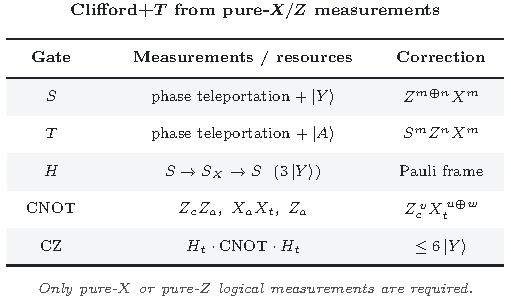
\includegraphics[width=\columnwidth]{gate_compilation.pdf}
\caption{Measurement-based compilation of $S$, $T$, $H$, CNOT, and CZ from pure-$X/Z$ logical measurements, $|Y\rangle$/$|A\rangle$ resources, and Pauli-frame updates.  The displayed circuits are ideal identities; their fault-tolerant realization uses the geometric and spacetime conditions developed in Secs.~\ref{sec:gauging}--\ref{sec:ft}.}
\label{fig:gate-compilation}
\end{figure}

The following formulas make the ideal logical gate algebra explicit. Fault-tolerant realization additionally depends on the geometric and spacetime conditions developed in Secs.~\ref{sec:gauging} and~\ref{sec:ft}. An outcome bit $m=0$ denotes eigenvalue $+1$, and $m=1$ denotes eigenvalue $-1$. Products of correction operators act from right to left. All formulas use pure-$X$ or pure-$Z$ measurements and Pauli frame updates. Output wires and candidate resource costs are specified below.

\paragraph{Phase teleportation.}
Let $R_\theta=\operatorname{diag}(1,e^{i\theta})$ and prepare an auxiliary logical qubit $a$ in $R_\theta|+\rangle$. Measure $Z_dZ_a$ with bit $m$, then $X_d$ with bit $n$, discard $d$, and retain $a$. Apply
\begin{equation}
 C_{mn}=R_{2\theta}^{\,m}Z_a^nX_a^m.
 \label{eq:phase-correction}
\end{equation}
The output is $R_\theta|\psi\rangle$ up to a global phase. For $\theta=\pi/2$ this implements $S$ using one $|Y\rangle$ with correction $Z^{m\oplus n}X^m$. For $\theta=\pi/4$ it implements $T$ using one $|A\rangle$, with correction $S^mZ^nX^m$. The possible $S$ correction uses at most one further $|Y\rangle$ and another phase teleportation. Preallocate that candidate resource when a branch-independent resource count is needed.

\begin{proof}
Write $|\psi\rangle=\alpha|0\rangle+\beta|1\rangle$. The unnormalized retained state after the two measurements is
\begin{align}
 m=0:&\quad \tfrac12\bigl(\alpha|0\rangle+(-1)^n e^{i\theta}\beta|1\rangle\bigr),\\
 m=1:&\quad \tfrac12\bigl((-1)^n\beta|0\rangle+e^{i\theta}\alpha|1\rangle\bigr).
\end{align}
Applying Eq.~\eqref{eq:phase-correction} gives respectively $R_\theta|\psi\rangle/2$ and $e^{i\theta}R_\theta|\psi\rangle/2$. Each branch has probability $1/4$, independent of the input, so the same identities hold with an arbitrary reference entangled with the input.
\end{proof}

\paragraph{An $X$-axis phase and a Hadamard.}
Define $S_X=HSH$. Prepare $a$ in $Z|Y\rangle$, measure $X_dX_a$ with bit $m$, then $Z_d$ with bit $n$. Retain $a$ and apply $X^{m\oplus n}Z^m$. This implements $S_X$ up to a global phase: it is the $X/Z$-exchanged phase-teleportation identity, since $H|Y\rangle=e^{i\pi/4}Z|Y\rangle$. Therefore the sequence
\begin{equation}
 S\ \longrightarrow\ S_X\ \longrightarrow\ S
\end{equation}
implements $H$ up to a global phase, because
\begin{equation}
 SS_XS=e^{i\pi/4}H.
\end{equation}
This uses three $|Y\rangle$ states and requires no physical Hadamard as an input primitive.

\paragraph{CNOT.}
For control $c$, target $t$, and ancilla $a$ initialized to $|+\rangle$, measure in this order
\begin{equation}
 Z_cZ_a\;(u),\qquad X_aX_t\;(v),\qquad Z_a\;(w).
\end{equation}
Discard $a$ and retain $(c,t)$. The correction is
\begin{equation}
 Z_c^vX_t^{u\oplus w}.
\end{equation}
For a direct verification, write $\Pi_m(P)=(I+(-1)^mP)/2$. The unnormalized branch map before correction is
\begin{equation}
 K_{uvw}=\langle w|_a\,\Pi_v(X_aX_t)\Pi_u(Z_cZ_a)\,|+\rangle_a.
\end{equation}
Expanding the two projectors gives
\begin{equation}
 Z_c^vX_t^{u\oplus w}K_{uvw}
   =\frac{e^{i\phi_{uvw}}}{2\sqrt2}\operatorname{CNOT}_{c\to t}
\end{equation}
for a branch-dependent global phase $e^{i\phi_{uvw}}$. This establishes the channel identity, with probability $1/8$ for each of the eight branches. No resource state is required.

\paragraph{CZ and universality.}
Apply $H_t$, then $\operatorname{CNOT}_{c\to t}$, then $H_t$. This implements CZ with at most six $|Y\rangle$ states using the preceding constructions. Together with preparation of $|0\rangle$ and $|+\rangle$, the verified CNOT, H, S and T formulas generate Clifford+T. All parity measurements involve at most two retained or ancillary logical qubits and can be scheduled as the one-block or two-block measurements covered by the architecture. Each teleported output must be assigned to its new logical wire and its Pauli frame carried forward.

\paragraph{Phase teleportation with a defective resource.}
The same computation with an arbitrary resource shows what a bad candidate
can do.  Let the auxiliary qubit $a$ and a system $E$ be in any joint state
$|\Phi\rangle_{aE}=|0\rangle_a|\phi_0\rangle+|1\rangle_a|\phi_1\rangle$ (a mixed
resource, or one entangled with other resources, is covered by taking $E$ to
contain a purifying system).  In
branch $(m,n)$ the retained state is, before correction,
\begin{equation}
 \tfrac{1}{\sqrt2}\sum_{b\in\{0,1\}}(-1)^{nb}\,\psi_b\,
 |b\oplus m\rangle_a\otimes|\phi_{b\oplus m}\rangle_E ,
 \label{eq:defective-teleport}
\end{equation}
where $|\psi\rangle=\psi_0|0\rangle+\psi_1|1\rangle$.  After $X_a^m$ this is
$\sum_b\psi_b|b\rangle_a\otimes|\epsilon_b\rangle_E$ for vectors
$|\epsilon_b\rangle$ independent of $\psi$, that is
$(I\otimes|\epsilon_+\rangle+Z\otimes|\epsilon_-\rangle)|\psi\rangle$ with
$|\epsilon_\pm\rangle=(|\epsilon_0\rangle\pm|\epsilon_1\rangle)/2$.  The
remaining corrections $R_{2\theta}^mZ^n$ are diagonal.  Hence, relative to the
ideal output $R_\theta|\psi\rangle$, every branch applies an operator in
$\operatorname{span}\{I,Z\}\otimes\mathcal B(\mathcal H_E)$ on the retained
wire, whatever the resource state and whatever it is entangled with.  The
same holds when the $S$ correction of a $T$ teleportation is itself
teleported with a defective $|Y\rangle$ slot, because a product of diagonal
operators is diagonal.  Section~\ref{sec:ft} uses this in place of a
resource-basis twirl (see Lemma~\ref{lem:defective-teleport}).

\paragraph{Algebraic verification.}
The script \texttt{reproducibility\_checks.py} evaluates all four $S$ branches, four $T$ branches, four $S_X$ branches, and eight CNOT branches.  It checks proportionality to the target unitary, branch probabilities, and the Hadamard composition to tolerance $10^{-12}$.  The script \texttt{resource\_defect\_check.py} checks Eq.~\eqref{eq:defective-teleport} for random resource states entangled with an environment.  The symbolic identities above establish the channel formulas, and the finite matrix checks provide reproducible cross-checks of every branch.


\section{Fault tolerance and universal architecture theorem}\label{sec:ft}
% Requires amsmath, amssymb, amsthm.

\paragraph{The argument in plain terms.}
This section is long because it handles every operation of the schedule, but
its shape is short, and the main text (Secs.~III~B and IV~A there) states it
in words.  An undetected logical error needs a fault pattern that no detector
notices.  Split such a pattern into pieces connected through common
detectors; at least one piece causes the error.  (i) A piece that lies inside
one operation and its surrounding idle rounds needs at least
$\min\{\beta_0d,R\}$ faults: either the errors it leaves form a logical of
the code at one time, every qubit of which carries a fault, or a wrong
outcome is repeated through all $R$ rounds
(Lemma~\ref{lem:relative-rectangle-distance} and the direct slice argument of
Proposition~\ref{prop:slice-bound}).  (ii) A piece that reaches from one
operation to the next must stay on one block for the whole padding between
them, and two connected faults are at most $\tau=O(1)$ rounds apart, so it
needs about $R_{\rm pad}/\tau$ faults (Lemma~\ref{lem:primitive-paths} and
Theorem~\ref{thm:padded-protected-composition}); the same lemma keeps the
neighborhoods of distinct resources $R/\tau$ apart
(Lemma~\ref{lem:resource-separation}).
(iii) To apply (i) without assuming perfect states at the start of an
operation, every time cut carries the syndrome, the logical frame, and the
last measurement records, and each piece is judged by its effect relative to
the fault-free evolution of that incoming data
(Lemmas~\ref{lem:rectangle-restriction} and~\ref{lem:contained-cut}).
(iv) Small courier blocks can expose only the resource they carry, and errors
created there are charged to the stage that creates them and then to
distillation (Lemmas~\ref{lem:encoded-courier-distance}
and~\ref{lem:earliest-stage-charging}).  (v) A minimum-weight decoder fails
only on a large connected set of fault locations, a fixed fraction of which
are faults, and counting such sets gives the threshold.
Figure~\ref{fig:ft-dependency} shows how the lemmas depend on each other.

\begin{center}
\fbox{\begin{minipage}{0.94\columnwidth}
\textbf{Detector convention.}  Physical detector vertices are only the bounded-support rows of $D^{\rm loc}$.  The full left-kernel space $\mathcal R^{\rm full}$ is used to check boundary algebra; its additional, possibly macroscopic relations are never inserted into the decoder graph or used as physical detectors.
\end{minipage}}
\end{center}

\paragraph{Conventions for faults and adaptive branches.}
A circuit location carries a finite set of nonidentity Pauli labels.  In the
local-stochastic Pauli model considered here, each faulty location is the ideal
operation followed by one selected Pauli on its support.  Thus a realized
fault set contains at most one mechanism above each circuit location.  If
$A$ is a set of mechanisms supported on distinct locations, local stochastic
noise means
\begin{equation}
  \Pr[F\supseteq A]\leq p^{|A|};                                      \tag{A1}
\end{equation}
if $A$ contains two labels above one location, the event on the left is empty.
We write $M$ for the total number of mechanism vertices and reserve $F$ for
the realized random set.

We formulate the decoder using a fixed causal location skeleton and a
\emph{local branch-uniform detector catalog}.  For a realized branch $h$ write
$D_h^{\rm loc}$ for the physical detector rows selected from that catalog,
$O_h$ for protected effects, and $\Gamma_h$ for the resulting fault graph.
Let $\Gamma_{\rm un}$ be the graph generated by the union of the same local
catalog over the finite branch alternatives.  Only $D^{\mathrm{loc}}$ defines
$\Gamma_h$, $\Gamma_{\rm un}$, connected components, cluster counting, the
temporal edge range $\tau$, or any separation length below.

This physical detector catalog is distinct from the algebraic closure of stabilizer relations at a code-deformation boundary.  For a
primitive $g$ with boundary check matrices $H_g^-$ and $H_g^+$ we write
\begin{equation}
 \mathcal R_g^{\mathrm{full}}:=\{(u,v):uH_g^-=vH_g^+\}.                 \tag{A2}
\end{equation}
The space $\mathcal R_g^{\mathrm{full}}$ is used only to audit the boundary-state
and gluing algebra.  Its elements are not, merely by virtue of belonging to
this left kernel, detector vertices of the fault graph.  In particular a
macroscopic stabilizer dependency is never inserted into $D^{\mathrm{loc}}$.
At a controlled location the classical history selects one operation from a
fixed finite list of bounded-support Clifford templates, and every branch
selects a subcollection of the fixed local detector catalog.  Thus the union
graph is fixed and has bounded degree without conditioning the local-stochastic
noise law on a prior global branch history.

\paragraph{Heterogeneous and biased Pauli rates.}
The single parameter $p$ in (A1) is only a domination parameter.  Suppose each
mechanism $a$ has a possibly location- and Pauli-dependent parameter $p_a$ and,
for every set $A$ of mechanisms on distinct circuit locations, the physical
distribution obeys
\begin{equation*}
 \Pr[F\supseteq A]\leq\prod_{a\in A}p_a,
 \qquad \sup_a p_a\leq p.
\end{equation*}
Then (A1) follows immediately, so every threshold and resource statement below
continues to hold with this $p$.  Thus arbitrary fixed Pauli bias, unequal
rates for gates, preparations, measurements and resets, and local correlations
already covered by this joint domination inequality require no change to the
proof.  Preparation and readout faults are explicit mechanisms in templates
T3--T5 of Sec.~\ref{sec:catalog}.  This observation does not extend the theorem to coherent CPTP faults
or leakage, which require additional arguments.

\begin{lemma}[Bounded fault-graph degree]\label{lem:A2}
There are constants $a_{\rm det},b_{\rm det},a_{\rm loc}<\infty$,
depending only on the fixed syndrome-extraction circuits, such that every
detector contains at most $a_{\rm det}$ circuit mechanisms, every mechanism
flips at most $b_{\rm det}$ detectors, and every circuit location has at most
$a_{\rm loc}$ Pauli labels.  Consequently
\begin{equation}
 \deg(\Gamma_{\rm un})
 \leq b_{\rm det}(a_{\rm det}-1)+a_{\rm loc}-1=:z=O(1).             \tag{A3}
\end{equation}
\end{lemma}
\begin{proof}
Each row of $D^{\mathrm{loc}}$ has bounded spacetime support by
Proposition~\ref{prop:uniform-local-detectors} below, so only locations in a
bounded neighborhood can flip it.  Conversely a Pauli at one
location propagates through only a bounded number of gates before the next
round boundary and hence flips only boundedly many detectors.  A neighbor of
a mechanism either has another label at the same location or shares one of
its at most $b_{\rm det}$ detectors, proving (A3).  The same bounds hold after
taking the union over the finite list of branch operations.
\end{proof}

\paragraph{Resource conventions.}
We use outcome bit $0$ for eigenvalue $+1$ and bit $1$ for eigenvalue $-1$.
Every compilation identity of Sec.~\ref{sec:gates} is understood as an equality of Kraus
maps, up to global phase, and specifies the retained output wire and its Pauli
frame.  Resource errors are described by defective subsystems rather than by
a fixed error basis (Definition~\ref{def:defective-family} below).

\paragraph{Uniform resource-state assumption.}
The resource layer uses only fixed-size logical factory codes and the same local layer-code primitives as the data path.  The Steane $7\!\to\!1$ and punctured Reed--Muller $15\!\to\!1$ circuits below do not grow with the target distance; their coordinates are implemented by protected logical operations on layer-code blocks, and distillation is iterated by moving candidate states through encoded courier stages of increasing block distance.  No perfect external magic-state source or nonlocal factory connectivity is assumed.  The sole distance-one exception is the raw injection boundary, which is isolated by the quotient-distance and earliest-stage charging lemmas before later encoded transfers are counted.

\paragraph{Explicit one-output factory primitives.}
We use the standard code-based $7\!\to\!1$ $|Y\rangle$ factory on the Steane
$[[7,1,3]]$ code and the $15\!\to\!1$ $|A\rangle$ factory on the punctured
Reed--Muller $[[15,1,3]]$ code \cite{Reichardt,BravyiKitaev,LitinskiMSD}.
At the logical level both are fixed in the same encode--transversal-phase--recover--decode form
\begin{equation}
 \mathcal F_Q=\mathrm{Dec}_Q\circ\mathcal R_Q\circ\mathrm{Syn}_Q
 \circ U_Q^{\rm tr}\circ\mathrm{Enc}_Q .                         \tag{A4a}
\end{equation}
For the Steane factory, $\mathrm{Enc}_Q$ prepares encoded $|+\rangle$ and
$U_Q^{\rm tr}$ is the fixed transversal $S/S^\dagger$ orientation that maps it to encoded
$|Y\rangle$; its seven physical phase gates are implemented by the
phase-teleportation identity of Sec.~\ref{sec:gates}, one preassigned
$|Y\rangle$ candidate per coordinate.  For the Reed--Muller factory,
$U_Q^{\rm tr}$ is the conventional transversal $T/T^\dagger$ layer of the
punctured Reed--Muller code, again implemented coordinatewise by the fifteen
preassigned $|A\rangle$ candidates; the fixed $T$ versus $T^\dagger$ convention
is absorbed into the known Clifford/frame convention of the factory.
$\mathrm{Syn}_Q$ extracts the CSS syndrome, $\mathcal R_Q$ applies a predetermined
minimum-weight Pauli recovery, and $\mathrm{Dec}_Q$ returns the single retained
logical output.  Thus the factory always produces an output rather than
postselecting; in the zero-error branch Eq.~(A4a) is exactly the standard ideal
$|Y\rangle$ or $|A\rangle$ factory map.  Tables~\ref{tab:steane-map}--\ref{tab:factory-map} give the coordinate matrices and the candidate-to-syndrome map used by $\mathcal R_Q$; \texttt{factory\_map\_audit.py} checks the ideal transversal phase orientation and writes \texttt{factory\_map\_audit.csv}.

\begin{definition}[Local-stochastic defective resource family]
\label{def:defective-family}
Let $\mathcal S$ be a finite set of resource slots, each an encoded logical
qubit that should hold an ideal resource $|R_i\rangle\in\{|A\rangle,|Y\rangle\}$
in the Pauli frame of the realized branch.  The family is
\emph{local-stochastic defective with parameter $q$} if its joint state, with
everything else in the computation collected into a system $E$, has the form
\begin{equation}
 \rho=\sum_{B\subseteq\mathcal S}\pi(B)\,
 \Bigl(\bigotimes_{i\notin B}|R_i\rangle\langle R_i|\Bigr)\otimes\sigma_{B,E},
 \tag{A4}
\end{equation}
where $\pi$ is a probability distribution with
$\sum_{B\supseteq A}\pi(B)\le q^{|A|}$ for every $A\subseteq\mathcal S$, and
each $\sigma_{B,E}$ is an arbitrary state of the defective slots $B$ together
with $E$.
\end{definition}

A defective slot may therefore hold any state, including a state entangled
with other defective slots, with data, or with the environment; no error basis
is assumed.  A good slot is exactly ideal and in tensor product with
everything else.

\begin{lemma}[Defective-resource phase teleportation]
\label{lem:defective-teleport}
In the phase-teleportation gadget of Sec.~\ref{sec:gates} with target
rotation $R_\theta$, replace the resource by an arbitrary state of the
auxiliary qubit and a system $E$.  Then in every measurement branch the
retained output equals $(R_\theta\otimes I_E)K$ applied to the input, with
$K\in\operatorname{span}\{I,Z\}\otimes\mathcal B(\mathcal H_E)$ independent of
the input state.  The same holds for $\theta=\pi/4$ when the conditional $S$
correction is teleported with an arbitrary $|Y\rangle$-slot state.
\end{lemma}
\begin{proof}
This is Eq.~\eqref{eq:defective-teleport} and the remark following it: after
the $X^m$ correction the retained state is
$\sum_b\psi_b|b\rangle\otimes|\epsilon_b\rangle_E$ with $|\epsilon_b\rangle$
independent of $\psi$, and the remaining corrections, and the $S$ correction
whether ideal or teleported with a defective slot, are diagonal in the
computational basis of the retained wire.
\end{proof}

\begin{lemma}[Single-defect recovery]\label{lem:A5}
Let $Q$ be the $[[7,1,3]]$ Steane code or the punctured $[[15,1,3]]$
Reed--Muller code used by the factory map (A4a), with the coordinatewise
convention of Tables~\ref{tab:steane-map} and~\ref{tab:rm-map}: the seven
Steane candidates and fifteen Reed--Muller candidates are assigned to
coordinates $i$, and a conditional sign-correction slot is assigned to the
same coordinate as the injection it corrects.  Call coordinate $i$ defective
if its principal candidate or its correction slot is defective.  Assume the
compiled nonresource operations of the run act as their ideal logical
channels.  If at most one coordinate is defective, the decoded output is
exactly the ideal resource and is in tensor product with all other systems,
whatever the states of the defective slots and whatever they are entangled
with.  Hence a defective output requires defective slots at two distinct
coordinates, and in particular at least two defective slots.
\end{lemma}
\begin{proof}
Condition on the branch of all teleportation outcomes.  By
Lemma~\ref{lem:defective-teleport}, good coordinates receive their ideal
rotation and the defective coordinate $i$ (if any) receives it followed by an
operator $I\otimes K_I+Z_i\otimes K_Z$ with $K_I,K_Z$ acting on the defective
slots and $E$ only.  The state after the transversal layer is therefore
$|\overline\psi\rangle\otimes|\kappa_I\rangle+Z_i|\overline\psi\rangle\otimes
|\kappa_Z\rangle$, where $|\overline\psi\rangle$ is the ideal encoded output.
The $X$-check syndrome of $Z_i$ is the nonzero column $v_i$ of
Tables~\ref{tab:steane-map} and~\ref{tab:rm-map}, and of $I$ it is zero, so
the syndrome measurement selects one of the two terms and the predetermined
recovery $\mathcal R_Q$ maps it to $|\overline\psi\rangle$.  The result is
$|\overline\psi\rangle\otimes|\kappa'\rangle$ in every branch, so the decoded
output is the ideal resource and carries no correlation with $E$.  Distinct
columns are needed only for two different coordinates; equivalently, if
$Z_i$ and $Z_j$ had the same syndrome then $Z_iZ_j$ would be a $Z$-type
normalizer element of weight two, hence a stabilizer since $d_Z(Q)\ge3$.
\end{proof}

All possible conditional correction resources are assigned in the fixed
schedule before a run, whether or not they will be used; each is produced
just before its coordinate is processed, and an unused one is discarded.  The
fixed assignment, not live storage, is what the lemmas need.  Each principal
or correction slot consumes a distinct candidate, and different distillation
runs use disjoint candidate sets, so no candidate is reused across
coordinates or runs.  If $c_Y$ is the
maximum number of conditional correction slots of a fifteen-to-one run
($c_Y=15$ for one $S$ correction per coordinate), set
\begin{equation}
 C_A=\tbinom{15+c_Y}{2},\quad C_Y=\tbinom{7}{2},\quad
 C_{\rm dist}=\max(C_A,C_Y).                                     \tag{A6}
\end{equation}

\begin{lemma}[Always-output distillation]\label{lem:A7}
Suppose the candidate slots at level $r$ form a local-stochastic defective
family with parameter $q_r$ (Definition~\ref{def:defective-family}), distinct
runs use disjoint slot sets, and the compiled nonresource operations act as
their ideal logical channels.  Then the outputs of the runs form a
local-stochastic defective family with parameter
\begin{equation}
 q_{r+1}\leq C_{\rm dist}\,q_r^2.                                 \tag{A8}
\end{equation}
\end{lemma}
\begin{proof}
Condition on the defective set $B$ of the input family.  By
Lemma~\ref{lem:A5}, every run whose slots meet $B$ in at most one coordinate
outputs its ideal resource in tensor product with everything else, whatever
$\sigma_{B,E}$ is.  Let $B'$ be the set of runs whose slots meet $B$ in at
least two slots.  Averaging over $B$ with fixed $B'$ gives a state of the
form (A4) for the outputs, with defective set $B'$.  If $B'\supseteq A'$,
then $B$ contains a pair of slots of each run in $A'$; these pairs are
disjoint, so a union bound over the at most $C_A$ or $C_Y$ pairs per run gives
$\sum_{B'\supseteq A'}\pi'(B')\le\prod_{u\in A'}C_u\,q_r^{2}\le
(C_{\rm dist}q_r^2)^{|A'|}$.  This proves (A8) without postselection, without
independence of resource errors, and without assuming any error basis for a
defective slot.
\end{proof}

No resource-basis twirl is used, and Lemmas~\ref{lem:A5} and~\ref{lem:A7} do
not need one (Sec.~\ref{sec:archive} records the twirl of an earlier version
and why it fails).  The script \texttt{resource\_defect\_check.py} simulates
both factories with one defective slot in an arbitrary state entangled with
an environment.  The decoded output equals the ideal output in every branch
of the Steane factory, and in sampled branches of the Reed--Muller factory
with every branch at the defective coordinate enumerated (good coordinates
contribute branch-independent ideal operations).  Defects at two coordinates
fail.

\paragraph{Injected resources form a defective family.}
Under the local-stochastic Pauli model, conditional on the realized fault set
every raw resource is $P_\iota|R\rangle$ for a Pauli $P_\iota$ (a fault after
the physical preparation or rotation is a Pauli, and a Pauli before the
rotation either acts trivially on $|+\rangle$ or becomes $Z$), every later
operation is a Clifford measurement circuit, and all frame updates are
Pauli.  In the realized frame each delivered resource is therefore
$P_\iota|R\rangle$ with $P_\iota$ the residual logical Pauli on the traveling
slot, and the joint state is a mixture over fault sets of product states.
Let $B$ be the set of sites with $P_\iota\neq I$; a site lies in $B$ exactly
when $E_\iota$ occurs.  Theorem~\ref{thm:A11}, Eq.~(A13), gives
$\Pr[B\supseteq A,\,G]\le q_{\rm inj}^{|A|}$, and conditioning on $G$ multiplies this
by at most two when $\Pr[G^c]\le1/2$, so
$\Pr[B\supseteq A\mid G]\le(2q_{\rm inj})^{|A|}$.  Grouping the mixture by $B$ puts it
in the form (A4) with parameter $q_0\le2q_{\rm inj}$.  Lemma~\ref{lem:A7} is then
applied level by level on $G$, which is contained in the event $G_{\rm res}$
on which every noninjection compiled operation acts as its ideal logical
channel (paragraph ``Residual components and the event $G_{\rm res}$''
below Theorem~\ref{thm:A11}).

\paragraph{A location-level committed-decoding bound.}
At commitment time $t_j$, the decoder uses all available branch detectors
through $t_j+b$ and selects a minimum-cardinality mechanism set with the
observed syndrome.  Every observable committed at $t_j$ is a parity of
outcomes available by $t_j$.  The mechanisms selected up to $t_j$ are
committed as the decoder's correction; the \emph{residual} is the symmetric
difference of the realized faults and the committed correction.

\begin{lemma}[Committed witness]\label{lem:A9}
If a committed observable is wrong, $\Gamma_{\rm un}$ contains a connected
set $S$ with $|S\cap F|\geq |S|/2$ such that either $S$ has empty full
syndrome and the corresponding observable effect, or
\begin{equation}
 |S|\geq 1+\left\lfloor\frac{b-\tau}{\tau}\right\rfloor,            \tag{A10}
\end{equation}
where adjacent mechanisms differ in time by at most $\tau$.
\end{lemma}
\begin{proof}
Symmetric-difference the realized prefix with the minimum-cardinality
correction and decompose it using adjacency through available detectors and
shared locations.  Each component has zero available syndrome.  Minimality
gives at least half realized faults in every component, since exchanging the
realized and corrected mechanisms of a component with fewer realized faults
would give a smaller correction with the same available syndrome; in
particular this holds for every component whose removal changes the
committed value.  Such a component either has no unavailable boundary
detector and hence zero full syndrome, or connects the causal support of the
observable at time at most $t_j$ to a mechanism within $\tau$ of the boundary
$t_j+b$.  A path in the union graph gives (A10).
\end{proof}

For an injection site $\iota$ let $E_\iota$ be the event that the resource
delivered at $\iota$ carries a nontrivial residual logical Pauli in the
realized frame, that is, that some connected component of the residual has
a nonzero effect on the traveling resource of $\iota$; we call this a wrong
injection commitment.

\begin{theorem}[Adaptive cluster bound with weighted injection certificates]
\label{thm:A11}
Suppose every noninjection observable has protected mechanism fault distance at least $f$, the
buffer obeys $b\geq\tau(f+1)$, and distinct injection neighborhoods have
union-graph distance at least $\rho$.  Partition each injection neighborhood
as $N_\iota=\bigcup_aN_{\iota,a}$.  Let $G$ be the event that
$\Gamma_{\rm un}$ contains no connected quarter-dense set (a set $S$ with $|S\cap F|\ge|S|/4$; \emph{half-dense} means $|S\cap F|\ge|S|/2$) of size at least
$f_\star:=\min(f,\rho)$.  Assume that, on $G$, every wrong injection
commitment $\iota$ has a connected half-dense witness anchored in some
$N_{\iota,a}$, of size at least $s_a$, and witnesses for distinct wrong sites
do not touch.  If $p\leq p_\star:=(4ez)^{-4}$, then
\begin{align}
 \Pr[G^c]&\leq4M(p/p_\star)^{f_\star/4},                            \tag{A12}\\
 \Pr\!\left[\bigcap_{\iota\in I}E_\iota\cap G\right]
 &\leq q_{\rm inj}^{|I|},                                                    \tag{A13}\\
 q_{\rm inj}&\leq \sum_a |N_{\iota,a}|
       \sum_{s\geq s_a}(ez)^{s-1}2^sp^{s/2}.                        \tag{A14}
\end{align}
The supremum of the right side of (A14) over $\iota$ is understood.
\end{theorem}
\begin{proof}
There are at most $M(ez)^{s-1}$ connected size-$s$ sets with a chosen anchor.
For a fixed set, (A1) and a union bound over subsets show that quarter density
costs at most $2^sp^{s/4}$.  All connected-set enumeration is performed in the
single fixed union graph $\Gamma_{\rm un}$ before reference to any realized
adaptive history; at no point is (A1) replaced by, or inferred for, a distribution
conditioned on a branch.  Summing the geometric tail gives (A12).  On $G$,
Lemma~\ref{lem:A9} and the distance hypotheses exclude all wrong noninjection
commitments.  A wrong injection witness of size at least $f$ would also have
been excluded; a smaller zero-syndrome witness is therefore assigned to its
unique injection neighborhood.  If two assigned witnesses touched, their
union would be connected, meet two neighborhoods, have size at least $\rho$,
and be quarter-dense, again contradicting $G$.

For fixed pairwise nontouching witnesses, choose at least half their vertices
as realized mechanisms.  These vertices lie at distinct physical locations,
including across witnesses, so (A1) applies and the sum factorizes.  Anchoring
in stage $a$, counting connected sets, and summing over sizes gives one factor
(A14) per site, proving (A13).  No independence of injection events is used.
\end{proof}

Conditioning on $G$ multiplies $q_{\rm inj}$ by at most two whenever
$\Pr[G^c]\leq1/2$.

\paragraph{Residual components and the event $G_{\rm res}$.}
Let $G_{\rm res}$ be the event that every noninjection compiled operation,
including memory between production and consumption of resources, acts as
its ideal logical channel: every committed outcome of a data or factory
operation is correct, and the residual has no component with a nonzero
effect on a data or factory logical other than a traveling resource slot.
(Raw and courier teleportation outcomes act only on the frame of the
traveling resource; a wrong one is part of the event $E_\iota$.)  The
effect of a component is evaluated at idle cuts placed around it, the right
one after a round free of it; by Lemma~\ref{lem:contained-cut} the component
leaves zero syndrome and zero records there, so its effect does not depend on
the choice of logical representatives.  With the parameter choice
$\alpha\min\{\beta_0d,R\}\ge f$ of (A19), used in Theorem~\ref{thm:A24},
$G\subseteq G_{\rm res}$.  Indeed, decompose the residual as in the proof of
Lemma~\ref{lem:A9}: by minimality every component is half-dense, and a
component either reaches the boundary of the available detectors, and then
$|S|\ge1+\lfloor(b-\tau)/\tau\rfloor\ge f+1$ by (A10) and $b\ge\tau(f+1)$, or
has zero full syndrome.  A component of the second kind with a nonzero effect
on a committed data or factory outcome, or on a data or factory logical away
from a resource boundary, has size at least $f$ by item~1 of
Theorem~\ref{thm:A16}.  At a resource boundary only the terminal transfer
touches a data or factory block (the raw stage and the courier stages $j<J$
involve dedicated courier blocks only), and there an effect on a logical of
the factory block other than the designated slot has size at least
$\alpha\min\{\beta_0d,R\}\ge f$ by item~2 of Theorem~\ref{thm:A16} and (A19).  In all
cases the component is a connected quarter-dense set of size at least
$f_\star$, which $G$ excludes.  Under Pauli noise, correct outcomes and
residual components without logical effect mean that the logical action is
the ideal one.  For the events $E_\iota$ the same decomposition, the
exclusion of the (A10) alternative, and items~3--5 of Theorem~\ref{thm:A16}
(stage sizes, anchoring in $N_{\iota,j}$, and nontouching) give the
half-dense witness hypothesis of Theorem~\ref{thm:A11}.

\paragraph{Canonical nearest-neighbor extraction schedule.}
We now fix the physical schedule rather than leave it as a certificate.  For
any CSS check set appearing in an idle, gauged, factory, birth, death, or
readout window, use local ancillas to measure all $Z$ checks and then all $X$
checks.  Theorem~\ref{thm:local-gauging} gives a uniform bound on
check weight, qubit/check incidence, and geometric diameter.

\begin{proposition}[Nearest-neighbor extraction from local templates]
\label{prop:nn-extraction}
There is a constant-depth nearest-neighbor syndrome-extraction schedule for
every check set in the canonical catalog.  A circuit Pauli fault in one such
round propagates to at most $c_1=O(1)$ phenomenological data-Pauli or
check-outcome mechanisms, uniformly in block size.
\end{proposition}
\begin{proof}
Let $R_*$ be a uniform radius containing the support of every check in the
fixed refined catalog.  Because the refinement is fixed and every support has
bounded size, reserve within the same ball one routing ancilla site and, for
each possible support label, a contact microvertex adjacent to that data qubit.
The number of such reserved sites is $O(1)$ per local geometry.  Choose the
lexicographically first spanning tree of the reserved routing graph, rooted at
the ancilla site, and move the ancilla label by nearest-neighbor SWAPs along a
depth-first traversal.  On the first visit to the contact microvertex assigned
to a support qubit, apply the required nearest-neighbor data--ancilla CNOT.
After the last interaction, retrace the traversal before readout, restoring all
moved labels to their canonical sites.

If $V_*$ is the maximum number of routing sites in such a ball and $w_0$ the
maximum check weight, one extraction word contains at most $2(V_*-1)$ shuttle
SWAPs, $w_0$ data--ancilla CNOTs, and $O(1)$ preparation/readout locations.
Hence its depth and fault light cone are bounded by a constant
$L_*=O(V_*+w_0)$ independent of block size.  Two extraction words conflict
only when their radius-$R_*$ balls overlap.  Bounded local density therefore
gives a bounded-degree conflict graph, so a constant coloring executes all
checks in $O(1)$ sequential color classes.  A circuit Pauli fault crosses at
most $O(L_*)$ subsequent local gates before the round boundary and consequently
produces at most $c_1=O(1)$ phenomenological mechanisms.  This canonical
construction fixes a nearest-neighbor route for every bounded local support.
\end{proof}

\paragraph{Finite single-fault audit.}
The ancillary script regression-tests the circuit-to-phenomenological reduction on both displayed T8 CSS master families by inserting every nonidentity Pauli at every preparation, CNOT, SWAP, and measurement location and propagating it through the remaining Clifford word.  The bundled audit covers check weights $1$--$8$ and reversible shuttle stress words of lengths $0$--$2$, totaling 10,008 single-location faults; its largest phenomenological image has weight $10$.  The companion \texttt{t8\_master\_routing\_catalog.csv} records all 48 audited words, including the operation word, return-to-canonical flag, location count, and per-word maximum fault image.  Proposition~\ref{prop:nn-extraction} supplies the complete routing construction analytically; these finite words provide executable regression tests of its local fault bookkeeping.

Adaptive corrections are compiled into preallocated slots.  The physical
slot at a spacetime cell is one member of a finite local catalog: idle
extraction, one- or two-block gauging, logical $X/Z$ readout, encoded
$|0\rangle/|+\rangle$ birth, encoded discard, raw injection,
or encoded courier transfer.  A fixed target logical circuit fixes the global
locations of these slots; classical outcomes only select among finite local
alternatives.

\begin{proposition}[Uniform local detector generation]
\label{prop:uniform-local-detectors}
For every canonical primitive $g$ and every branch, there is a physical
matrix $D_g^{\mathrm{loc}}$ and constants
$r_{\rm det},a_{\rm det},b_{\rm det}=O(1)$, independent of block size, such
that: (i) each detector row is contained in a radius-$r_{\rm det}$ spacetime
ball; (ii) each row touches at most $a_{\rm det}$ phenomenological mechanisms;
and (iii) each mechanism touches at most $b_{\rm det}$ detector rows.
The catalog is generated by finitely many local cell/template types.  It does
not contain an arbitrary basis of $\mathcal R_g^{\mathrm{full}}$.
\end{proposition}
\begin{proof}
Section~\ref{sec:catalog} displays the catalog as master templates T0--T8 rather
than only naming template classes.  T0 is the consecutive-round row
$[1\;1\mid\chi_C]$ for a persistent check; T1 is a bounded same-slice
meta-check; T2 is the explicit bounded merge/split row; T3 and T4 are the
gauging entry and exit rows involving $s_j$, $\widetilde s_j$, $B_p$, and
edge preparation/readout bits; T5 gives one-sided birth/readout endpoints;
and T6 states that injection/courier/factory slots introduce no new row
species.  The banded matrix T7 displays an entire modified-check timeline, and
T8 gives the nearest-neighbor ancilla/SWAP/CNOT circuit words generated by the canonical spanning-tree shuttle construction.  These are the
same local detector generators used in the spacetime-code construction of
Ref.~\cite{WilliamsonYoderGauging}, supplemented by bounded same-slice local
relations when present.

There are only finitely many labeled local geometries after the fixed
refinement.  Hence the displayed templates have uniform maxima for row
diameter and row mechanism count, defining $r_{\rm det}$ and $a_{\rm det}$.
Conversely a mechanism can affect only displayed circuit words whose supports
meet a fixed-radius neighborhood of that mechanism.  Bounded qubit/check
density and bounded template depth therefore give a uniform column-incidence
bound $b_{\rm det}$.  Raw injection, encoded courier, and factory slots
are finite compositions of these same rows.  The constants depend on this
finite physical catalog, not on the dimension of the block-dependent full
relation space.
\end{proof}

Propositions~\ref{prop:nn-extraction} and~\ref{prop:uniform-local-detectors}
justify Lemma~\ref{lem:A2}; in particular the fault graph is the graph of
$D^{\mathrm{loc}}$, not of $\mathcal R^{\mathrm{full}}$.

\paragraph{Boundary-state linearization and algebraic closure.}
Fix one realized causal branch.  At every cut between adjacent catalog
primitives choose an independent stabilizer generating set and a complete
symplectic logical Pauli basis for every retained encoded block.  For a Pauli
deviation $P$ at that cut let $s(P)$ be its stabilizer-syndrome vector and
$\lambda(P)$ the vector of its commutators with the chosen logical
representatives, taken in the Pauli frame of the realized branch (outcome-dependent
byproducts, such as the gauging byproduct fixed by the edge readouts, are
applied to the frame).  The pair $(s,\lambda)$ determines the Pauli class
modulo the boundary stabilizer group: the kernel of $P\mapsto(s(P),\lambda(P))$
is exactly that stabilizer group.  We use deviations from the ideal branch, so
all relations are homogeneous over $\mathbb F_2$.

\paragraph{Quantum class and classical record.}
The pair $(s,\lambda)$ describes the quantum state at a cut; it does not
describe the measurement record.  For one persistent check $C$, let $f_t$ be
the data deviation before round $t$ and $\mu_t$ the flip of its record in
round $t$.  The physical syndrome, the reported record (as a deviation from
the ideal record) and the detector are
\begin{equation}
 s_t=s_{t-1}+\chi_C(f_t),\qquad r_t=s_t+\mu_t,\qquad d_t=r_{t-1}+r_t,
 \tag{A15-rec}
\end{equation}
so $d_t=\mu_{t-1}+\mu_t+\chi_C(f_t)$ is the T0 row of the catalog.  A row that
compares the last record before a cut with the first record after it (a T0
row of a persistent check, or a T2--T4 transition row) therefore reads the
record flip $\mu$ of the last round before the cut.  That flip is classical
data: it is not a function of the Pauli class, and it cannot be absorbed into
$s$.  At every cut we therefore also carry the vector $\rho$ of reported-record
deviations of the last round before the cut, one entry for each check measured
in that round; in a fault-free round $\rho=\Pi s$, where $\Pi$ maps $s$ to the
syndromes of the checks measured in that round, and in general
$\rho=\Pi s+\mu_\partial$ with $\mu_\partial$ the record flips of that round.  Every
catalog row compares at most two consecutive rounds, so records of earlier
rounds never enter a row that straddles a cut.  The complete boundary
variable at a cut is $(s,\lambda,\rho)$.

The frame coordinate depends on the chosen representatives whenever
$s(P)\neq0$.  With stabilizer $X_1X_2$, the operators $X_1$ and $X_2$
represent the same logical class, but $Z_1$ anticommutes with the first and
commutes with the second; changing representatives changes $\lambda(Z_1)$ by
the syndrome bit.  In general, if an output representative pulled back
through the ideal primitive equals the input representative times the
stabilizer product $\prod_iS_i^{c_i}$, the frame acquires $\sum_ic_is_i$.

For a primitive $g$, let $e_g$ be its phenomenological fault vector, $\delta_g$
the values of its detector rows (the rows whose later record lies in $g$,
including the rows that straddle its input cut), and $o_g$ its protected
committed outcomes.  Propagation through the fixed Clifford measurement
schedule gives
\begin{align}
 \delta_g&=D_g^{\mathrm{loc}}e_g+A_g^{\mathrm{loc}}s_g^{\rm in}
   +P_g^{\mathrm{loc}}\rho_g^{\rm in},                                  \tag{A15a}\\
 \lambda_g^{\rm out}&=L_g\lambda_g^{\rm in}+C_gs_g^{\rm in}+E_ge_g,             \tag{A15b}\\
 o_g&=Q_g\lambda_g^{\rm in}+G_gs_g^{\rm in}+F_ge_g,                             \tag{A15c}
\end{align}
together with the output boundary variables
\begin{equation}
 s_g^{\rm out}=\Sigma_g(s_g^{\rm in},\lambda_g^{\rm in})+J_ge_g,\qquad
 \rho_g^{\rm out}=\Pi_gs_g^{\rm out}+M_ge_g,                           \tag{A15a$'$}
\end{equation}
where $\Pi_g$ expresses the syndrome of each check of the last round through
the generating set and $M_g$ picks out the record flips of that round.  A
fault pattern is detector-trivial when every $\delta_g$ vanishes.  In a
fault-free inherited state $\rho^{\rm in}=\Pi s^{\rm in}$ and the input rows
of (A15a) vanish, so an inherited syndrome is not a detection event; an
inherited record error, $\rho^{\rm in}\neq\Pi s^{\rm in}$, is.  The committed
outcomes of the catalog are parities of records measured inside the primitive,
so $o_g$ does not depend on $\rho_g^{\rm in}$.

The matrices $C_g$ and $G_g$ are fixed by the ideal branch and the
representatives chosen at the two cuts.  Linearity does not force them to
vanish.  For a unitary primitive one may choose the output representatives as
the images of the input ones, which gives $C_g=0$; a code deformation
generally has to multiply the pushed-forward representatives by input
stabilizers to make them commute with the new checks, so we retain $C_g$ and
$G_g$ throughout.  Separately, embed the two boundary check groups in their
common qubit set, adjoining known product-state stabilizers at births and
final readout observables at deaths.  The full transition-relation space is
the algebraic closure $\mathcal R_g^{\mathrm{full}}$ of Eq.~(A2).  Section~\ref{sec:catalog}
lists both objects
explicitly: the local template catalog is used for decoding, whereas the full
left kernel is used only as an algebraic audit of boundary relations.

\begin{proposition}[Local generators suffice for boundary restriction]
\label{prop:local-suffices}
For every canonical transition, the rows of $D_g^{\mathrm{loc}}$ together with the
complete boundary variables $(s,\lambda,\rho)$ contain every constraint required
to restrict and glue the physical detector/effect system.  Every local
merge/split or endpoint parity used by the scheduled-circuit proof is a row of
this local catalog.  An additional element of
$\mathcal R_g^{\mathrm{full}}$ is a derived algebraic relation among ideal boundary
checks; it is not added as a fault-graph detector vertex.
\end{proposition}
\begin{proof}
Unchanged checks are connected across a transition by same-check local
comparisons.  Where the check set changes, the transition is a tiling by the
finite local merge/split, grid-plaquette, birth, readout, or courier endpoint
templates listed in Sec.~\ref{sec:catalog}.  These are precisely the local
parities used by the cleaning and rectangle arguments.  The variables
$(s,\lambda)$ record the residual Pauli class at the cut, and $\rho$ records
the classical data that the rows straddling the cut read, so no
perfect-boundary condition or macroscopic parity row is needed to continue
propagation into the next primitive.  Summing local identities may of course
produce further elements of $\mathcal R_g^{\mathrm{full}}$, and the full left
kernel enumerates all such algebraic relations, including possible
macroscopic dependencies.  Such derived relations supply no additional
physical measurement record and therefore remain in the algebraic audit space
rather than in $D_g^{\mathrm{loc}}$ or the fault graph.
\end{proof}

\begin{lemma}[Canonical local detector/effect gluing]
\label{lem:canonical-gluing}
For the canonical schedule, the global \emph{physical} detector/effect system
on a realized causal branch is the fiber product of the primitive systems
(A15a)--(A15c) and (A15a$'$), obtained by identifying the complete
$(s,\lambda,\rho)$ variables on every retained wire.  This exact gluing uses
$D^{\mathrm{loc}}$ for detector rows and does not require promoting the full
relation space to physical detectors.
\end{lemma}
\begin{proof}
A Clifford circuit with Pauli faults is linear on Pauli classes.  At a cut,
$(s,\lambda)$ is a complete coordinate for that class modulo stabilizers, so
the future quantum evolution, and hence every future record and logical
effect, depends on the past faults only through these variables.  A future
detector row can in addition read records measured before the cut; every
catalog row compares at most two consecutive rounds, so the only such records
are those of the last round before the cut, which are $\rho$.  Conversely each
physical detector row belongs to one bounded slot template of
Proposition~\ref{prop:uniform-local-detectors}; all cross-slot dependence is
therefore mediated by the retained boundary variables.  Identifying them and
eliminating internal ones reproduces exactly the physical circuit equations.
Proposition~\ref{prop:local-suffices} ensures that every local merge/split
parity needed by the schedule is present.  The full space
$\mathcal R_g^{\mathrm{full}}$ may be used to check the algebraic consistency of
this boundary description, but its extra derived rows are not required for,
and are not inserted into, the fiber product of physical detector rows.
\end{proof}

\paragraph{Worked gluing example (two adjacent idle primitives).}
\label{ex:gluing-two-idle}
The following miniature illustrates the boundary variables; it does
\emph{not} replace the general proof of Proposition~\ref{prop:local-suffices}
or Lemma~\ref{lem:canonical-gluing}.  Take a single persistent check $C$ and
two consecutive idle primitives $g_1,g_2$ of one round each, glued on the
mid-cut, with fault bits $e_t=(f_t,\mu_t)^\top$ (data Pauli anticommuting with
$C$ and with the logical partner, and record flip).  The boundary variables
are the syndromes $s_{\rm in},s_{\rm mid},s_{\rm out}$, the last-round records
$\rho_{\rm in},\rho_{\rm mid},\rho_{\rm out}$, and the frames
$\lambda_{\rm in},\lambda_{\rm mid},\lambda_{\rm out}$.  By (A15-rec) the two
primitives are
\begin{equation}
\begin{aligned}
 g_1:&\quad \delta_1=\rho_{\rm in}+s_{\rm in}+f_1+\mu_1,\quad
       s_{\rm mid}=s_{\rm in}+f_1,\\
     &\quad \rho_{\rm mid}=s_{\rm mid}+\mu_1,\quad
       \lambda_{\rm mid}=\lambda_{\rm in}+f_1,\\
 g_2:&\quad \delta_2=\rho_{\rm mid}+s_{\rm mid}+f_2+\mu_2,\quad
       s_{\rm out}=s_{\rm mid}+f_2,\\
     &\quad \rho_{\rm out}=s_{\rm out}+\mu_2,\quad
       \lambda_{\rm out}=\lambda_{\rm mid}+f_2.
\end{aligned}
\tag{A15-ex1}
\end{equation}
Eliminating $(s_{\rm mid},\rho_{\rm mid},\lambda_{\rm mid})$ gives
\begin{align}
 \delta_1&=\rho_{\rm in}+s_{\rm in}+f_1+\mu_1,\qquad
 \delta_2=\mu_1+f_2+\mu_2,
 \tag{A15-ex2}\\
 s_{\rm out}&=s_{\rm in}+f_1+f_2,\qquad \rho_{\rm out}=s_{\rm out}+\mu_2,
 \nonumber\\
 \lambda_{\rm out}&=\lambda_{\rm in}+f_1+f_2,
 \tag{A15-ex3}
\end{align}
which are the detector/effect equations of the two-round idle circuit on $C$
written directly.  The syndrome is a quantum variable and changes only with
$f$; the records carry $\mu$.  For $f_1=f_2=0$, $\mu_1=\mu_2=1$ and
$s_{\rm in}=\rho_{\rm in}=0$, the syndrome is zero at every cut,
$\rho_{\rm mid}=\rho_{\rm out}=1$, and a clean following round gives the
detector history $(1,0,1)$.  Gluing with $(s,\lambda)$ alone, that is, setting
$\rho_{\rm mid}=s_{\rm mid}$, would miss the $\mu_1$ term of $\delta_2$.  The
ancillary script \texttt{glue\_example\_check.py} verifies the fiber-product
identity on all $2^7$ assignments of
$(f_1,\mu_1,f_2,\mu_2,s_{\rm in},\rho_{\rm in},\lambda_{\rm in})$, the history
$(1,0,1)$, and that $(s,\lambda)$-only gluing disagrees exactly when
$\mu_1=1$.

\paragraph{Direct versus composed map on explicit blocks.}
The script \texttt{boundary\_composition\_check.py} tests
Lemma~\ref{lem:canonical-gluing} on the paper's own objects.  Two explicit
$[[4,2,2]]$-input blocks ($s=2$, $448$ data qubits) with the spanning grid of
Sec.~\ref{sec:two-block} ($184$ edge qubits) run the schedule
idle$\,\to\,$gauging$\,\to\,$idle$\,\to\,$gauging$\,\to\,$idle, each gauging
primitive consisting of an undeformed entry round, edge preparation, two
deformed rounds measuring $\overline X_1^{(a)}\overline X_1^{(b)}$, edge
readout, and an undeformed exit round.  The detectors are the catalog rows
T0, T3 and T4 ($6462$ rows, all deterministic in the noiseless circuit).  The
\emph{direct} map is a Stim frame simulation of the complete schedule in the
phenomenological model (each check measured as a multi-qubit Pauli product,
with data and edge Paulis, record flips and edge-readout flips as the fault
mechanisms);
the \emph{composed} map simulates each primitive in isolation from
$(s,\lambda,\rho)$ alone, with the logical representatives changed at every
cut so that the terms $C_gs$ are exercised.  For every one of the $20{,}000$
single phenomenological fault mechanisms, and for every unit inherited input
$(s_0,\lambda_0,\rho_0)$ at the first cut ($896$ inputs), the two maps agree on
all detectors, both reported measurement bits, and the final boundary
variables; by linearity the maps are equal, including inherited syndromes and
record errors at the cuts.  Gluing with $(s,\lambda)$ only disagrees on
exactly the $1776$ record flips in the last round before the four internal
cuts, and the pattern of record flips on both sides of a cut gives
the history $(1,0,1)$ in both maps.

\begin{lemma}[Componentwise local-detector triviality]
\label{lem:componentwise}
Let the phenomenological fault graph join mechanisms when they share a row of
$D^{\mathrm{loc}}$ or the same physical location.  If a global fault vector has
zero local-detector syndrome, every connected component of its support
separately has zero local-detector syndrome.
\end{lemma}
\begin{proof}
All mechanisms appearing in one row of $D^{\mathrm{loc}}$ are pairwise adjacent.
Hence the nonzero mechanisms contributing to one detector row lie in a single
connected component.  The global parity of that row is zero, so its parity in
that component is zero.  This holds for every local detector row.
\end{proof}

\begin{lemma}[Rectangle restriction for the canonical schedule]
\label{lem:rectangle-restriction}
Let $C$ be a connected component of a globally $D^{\mathrm{loc}}$-trivial fault
pattern and suppose its temporal span intersects at most one active primitive.
Choose cuts in the surrounding idle pads containing every mechanism of $C$.
After all other components are set to zero, there exist inherited boundary
variables $(s_L,\lambda_L,\rho_L)$ and $(s_R,\lambda_R,\rho_R)$ for which the
restricted subchain is a valid relative rectangle solution with exactly the
protected relative effect contributed by $C$.  No condition $s_L=s_R=0$ or
$\rho_L=\rho_R=0$ is imposed.
\end{lemma}
\begin{proof}
Lemma~\ref{lem:componentwise} makes the mechanism vector of $C$ locally
detector-trivial by itself.  Apply Lemma~\ref{lem:canonical-gluing} with every
other mechanism set to zero.  The resulting global solution supplies
definite boundary variables at each cut; retaining only the variables in the
chosen subchain preserves all local primitive and gluing equations.
Equations (A15a)--(A15c) are linear, so subtracting the fault-free propagation
of the same left boundary variables, including the terms $A_gs_L$,
$P_g\rho_L$, $C_gs_L$ and $G_gs_L$, leaves exactly the contribution of $C$.
Thus a nonzero inherited syndrome, or an inherited record error, can cross
either artificial cut without being reinterpreted as a new fault.  When the
cuts lie in idle pads, contain every mechanism of $C$, and the right cut
follows a round that contains no mechanism of $C$,
Lemma~\ref{lem:contained-cut} shows in addition that $s_L=\rho_L=0$ and
$s_R=\rho_R=0$.
\end{proof}

\begin{lemma}[Contained components leave no cut syndrome or record]
\label{lem:contained-cut}
Let $C$ be a detector-trivial connected component and let two cuts lie in
idle rounds of every block that $C$ touches, with every mechanism of $C$
strictly between them and at least one complete round containing no mechanism
of $C$ immediately before the right cut.  With all other components set to
zero, the boundary variables propagated by $C$ have $s=0$ and $\rho=0$ at both
cuts.  Consequently the global protected effect of $C$ equals its relative
effect (A15-rel) in the enclosed subchain, and the terms $A_gs$, $P_g\rho$,
$C_gs$ and $G_gs$ never contribute to a contained component.
\end{lemma}
\begin{proof}
At the left cut no mechanism has occurred, so $(s_L,\lambda_L,\rho_L)=0$; a
block born inside the subchain has no left variables and receives the fixed
product-state input.  At the right cut take any check of the boundary
generating set of a retained block, and let $t^\ast$ be the last round before
the cut, which contains no mechanism of $C$.  The check's record in round
$t^\ast$ is linked to the left cut, or to the birth of its block, by a chain of
local detector rows.  Within idle and deformed windows the chain consists of
consecutive T0 rows; at a deformation it uses the T3a entry row and the T4a
exit row.  At a merge or split, an output check whose value is fixed by the
input checks is chained back through its T2 row to the chains of those
inputs; for the remaining, genuinely new output checks, the first records of
a basis fix the realized frame, so their chains start there with value zero.
At a birth the chain ends on the T5a row of a check with deterministic
initial value, which plays the role of $\rho_L=0$; for a check whose first
record after birth is random, that record fixes the realized frame in the
same way.  Every
row of the chain is satisfied because $C$ is detector-trivial.  Summing the
chain telescopes by (A15-rec): each interior record occurs in two
consecutive rows and cancels.  The terms that occur only once are
$\rho_L=0$, the record $r_{t^\ast}$, the preparation bits of a T5a birth row,
and, for a check $s_j$ deformed in a gauging window, the edge terms of its T3a
and T4a rows, whose sum over $e\in\mu_j$ is the deviation of the reported edge
readouts on $\mu_j$.  Add the T3b, T0 and T4b rows of the flux checks of a
2-chain of unit squares and parallel-copy cycles whose boundary is $\mu_j$
plus the tree path joining the ports of $s_j$ (these checks generate the
cycle space of the grid).  Each flux chain contributes the reported-readout
deviation around its cycle, so this replaces the sum over $\mu_j$ by the
reported-readout deviation along the tree path, which is the commutator of
the gauging byproduct with $s_j$.
The telescoped sum is therefore the record of the check in round $t^\ast$ in
the realized frame, and it vanishes.  No record flip of $C$ occurs in round
$t^\ast$, so $s_{t^\ast}=r_{t^\ast}=0$, and no data mechanism of $C$ occurs
after round $t^\ast$, so $s_R=s_{t^\ast}=0$ and $\rho_R=r_{t^\ast}=0$.  A block
discarded inside the subchain has no right variables; its protected readout
outcome is part of the relative effect.  The global effect of
$C$ is the fault-free propagation of $(0,\lambda_R,0)$ through the rest of the
circuit, which is determined by $\lambda_R$ alone; and $\lambda_R$, together
with the recorded outcomes inside the subchain, is the relative effect of $C$
because the incoming variables are zero.  The exhaustive check in
\texttt{frame\_propagation\_check.py} confirms $s=0$ at the output cut on all
$2^{16}$ patterns of a two-check, four-round idle window when a fault-free
round follows the cut, and \texttt{boundary\_composition\_check.py} confirms
the record-aware gluing on explicit blocks.
\end{proof}

\paragraph{Relative local rectangle distance.}
For a primitive or macro-rectangle with incoming variables
$(s,\lambda,\rho)$, define its \emph{relative} detector values and protected
effects by subtracting the fault-free propagation of the same incoming
variables:
\begin{equation}
\begin{aligned}
 \Delta\delta&=\delta+A s^{\rm in}+P\rho^{\rm in},\qquad
 \Delta\lambda=\lambda^{\rm out}+L\lambda^{\rm in}+Cs^{\rm in},\\
 \Delta o&=o+Q\lambda^{\rm in}+Gs^{\rm in}.
\end{aligned}
 \tag{A15-rel}
\end{equation}
Because the circuit is linear on Pauli deviations,
$(\Delta\delta,\Delta\lambda,\Delta o)=(De,Ee,Fe)$ depends only on the internal
fault vector, not on the inherited boundary variables.  Without the
$Cs^{\rm in}$ and $Gs^{\rm in}$ terms this independence fails: on an explicit
layer-code block whose two cuts use slab representatives at different heights,
the reduced law $\lambda^{\rm out}=L\lambda^{\rm in}$ fails for $986$ of $1979$
random inherited deviations with nonzero syndrome, while (A15b) holds for all
$2000$ and (A15-rel) returns the internal effect in every case
(\texttt{frame\_propagation\_check.py}).  Without the $P\rho^{\rm in}$ term an
inherited record error would be charged to the rectangle as a detection
event of its own faults.

\paragraph{Relative spacetime cleaning.}
Williamson--Yoder Theorem~4 (fault tolerance), with the detailed
spacetime-code statement in Theorem~5 (spacetime fault-distance) of their
Supplementary Information and its Lemmas~4--7 (spacetime code, local spacetime
stabilizers, time fault-distance, decoupling of space and time faults), in the
published version of Ref.~\cite{WilliamsonYoderGauging}, lower-bounds the
gauging fault distance by separating detector-trivial histories into
spacelike and timelike representatives.  We
use that cleaning argument through the explicit WY1--WY6 interface below,
adapted to inherited boundary classes.  Table~\ref{tab:cleaning-map} gives the
one-to-one correspondence with the present local detector schedule.

\begin{proposition}[Spacetime-cleaning interface for the canonical schedule]
\label{prop:cleaning-interface}
Consider one ordinary gauging macro-rectangle, including its undeformed entry
round, $R_g$ repeated deformed-code rounds, and undeformed exit round.  Let
$\mathcal C_0$ and $\mathcal C_g$ be the undeformed and deformed check sets.
The spacetime-cleaning theorem of Ref.~\cite{WilliamsonYoderGauging} applies
to the relative problem used here because the following hypotheses hold.
\begin{enumerate}
\item[\textup{(WY1)}] The detector set contains consecutive-round comparison rows for every
check repeated within $\mathcal C_0$ or $\mathcal C_g$, the local
undeformed--deformed entry rows, and the local deformed--undeformed exit rows.
Bounded same-slice relations, when present, are included as additional local
detectors.
\item[\textup{(WY2)}] For every physical qubit and every adjacent pair of time slices, the
usual local spacetime stabilizer exists: equal Pauli faults on the two slices,
together with measurement faults on precisely the intervening checks that
anticommute with that Pauli.  At entry and exit the corresponding
initialization/readout versions exist.  These moves are detector-trivial and
have zero protected relative effect.
\item[\textup{(WY3)}] The deformed check set is repeated for exactly $R_g$ complete rounds, so
a genuinely timelike measurement fault must connect the two deformation
boundaries and has phenomenological weight at least $R_g$.
\item[\textup{(WY4)}] Every nontrivial spacelike protected class of the deformed code has
weight at least $d_g^{\rm space}\geq\beta_0d$.
\item[\textup{(WY5)}] The incoming boundary variables $(s,\lambda,\rho)$ are held fixed.
Hence the relevant quantity is the relative detector pattern and output
effect, not an absolute syndrome condition at an artificial perfect cut.
\item[\textup{(WY6)}] Phenomenological weight counts one for each data-Pauli,
initialization/readout, or check-record mechanism.  Cleaning preserves the
parity of occupied space/initialization faults on every fixed spatial
timeline.  Consequently, if cleaning leaves $w$ occupied spacelike timelines,
the original fault vector has weight at least $w$.
\end{enumerate}
Under these hypotheses every detector-trivial fault vector with nonzero
relative protected effect is equivalent, by multiplication with local
spacetime stabilizers, to a product of a spacelike protected fault and a
purely timelike fault.  Therefore its weight is at least
$\min\{d_g^{\rm space},R_g\}$.
\end{proposition}
\begin{proof}
We verify the six cleaning conditions directly in the present detector and boundary notation.  For WY1, template T0 of Sec.~\ref{sec:catalog} is the repeated-check
detector of the gauging spacetime code; T3 and T4 are respectively the
initialization/deformation and deformation/readout detector rows, including
the $B_p$ and $\widetilde s_j$ endpoint parities.  Template T1 adds only
bounded space-only local relations.  This is exactly the modification allowed
when a code has local meta-checks: adding valid detector rows cannot create a
new detector-trivial fault.

For WY2, the fixed bounded-depth extraction circuit gives the standard
adjacent-time spacetime stabilizers locally.  A Pauli $P$ inserted on a qubit
at time $t$ and the same $P$ at $t+1$, together with flips of the intervening
check records that anticommute with $P$, changes neither any physical detector
nor the propagated encoded Pauli class.  At the deformation boundaries an
edge-initialization fault is paired with the corresponding first-slice Pauli,
and a last-slice Pauli is paired with the corresponding edge readout fault.
These are precisely the local generators used in the spacetime-stabilizer
construction of Ref.~\cite{WilliamsonYoderGauging}.  Because they are actual
identity moves of the recorded Clifford schedule, they remain trivial for the
additional T1 local-dependency detectors as well.

WY3 is part of the canonical macro-rectangle definition.  Once the
spacelike Pauli support has been cleaned to one time slice, any residual
measurement-only logical is a temporal string with endpoints on the start and
end of the deformation window.  Consecutive-check detectors force such a
string through all $R_g$ repeated rounds, so it contains at least $R_g$
measurement/init/readout mechanisms.  WY4 is exactly the static distance
statement of Theorem~\ref{thm:local-gauging}; the corresponding
idle-memory value is $d$.

For WY5, Proposition~\ref{prop:local-suffices} and
Lemma~\ref{lem:rectangle-restriction} allow arbitrary inherited
variables $(s,\lambda,\rho)$ at the left cut and compare the faulty rectangle
with the fault-free propagation of the same variables, including the syndrome
and record terms of Eq.~(A15-rel).  Subtracting the two solutions
therefore produces the zero-input relative problem required by cleaning,
without imposing $s=0$ at a real boundary.

Finally, the weight step in WY6 is the point that prevents a hidden
weight-increasing projection.  The adjacent-time generators let us sweep every
paired data-Pauli occupation forward or backward along its spatial timeline.
At the first and last slices, the entry/exit versions terminate exactly the
occupations paired with the corresponding preparation/readout variables.
After this elimination, choose one reference slice and sweep every remaining
non-endpoint data occupation to that slice.  What remains separates into (i) a
single-slice Pauli representative carrying the spacelike protected class and
(ii) record/init/readout variables only.  Consecutive-round detector equations
force any nontrivial part of (ii) to form a temporal chain from one deformation
boundary to the other; otherwise its first or last endpoint would flip a local
T0/T3/T4 detector.  Hence the temporal part has weight at least $R_g$.

The same sweep preserves mod-2 occupancy on each fixed spatial timeline.
Every occupied timeline in the single-slice representative therefore contains
at least one mechanism of the original fault vector, including the endpoint
convention.  If the spacelike part has nonzero protected effect it has at least
$d_g^{\rm space}$ occupied timelines; if it is protected-trivial, all nonzero
relative effect resides in the temporal part and costs at least $R_g$.  If both
parts are present, either lower bound already applies to the original vector.
Thus the desired relative distance is at least
$\min\{d_g^{\rm space},R_g\}$.  This is the Williamson--Yoder cleaning
argument written directly in the present boundary and detector notation; the
citation supplies its original spacetime-code formulation rather than an
additional unverified hypothesis.
\end{proof}

\begin{table*}[t]
\caption{Correspondence between the Williamson--Yoder spacetime-cleaning ingredients and the canonical schedule used here.  The final column records the two extensions needed for the present circuit: bounded local dependency rows and inherited boundary classes.}
\label{tab:cleaning-map}
\scriptsize
\setlength{\tabcolsep}{4pt}
\renewcommand{\arraystretch}{1.15}
\begin{tabular}{@{}p{1.1cm}p{2.6cm}p{4.8cm}p{6.8cm}@{}}
\toprule
Label & Williamson--Yoder ingredient & Verification in this manuscript & Modification in the present schedule \\
\midrule
WY1 & Local consecutive-round and deformation-boundary detectors (spacetime-code generators) & Proposition~\ref{prop:cleaning-interface}, WY1; Proposition~\ref{prop:uniform-local-detectors}; templates T0, T3, T4 and banded matrix T7 of Sec.~\ref{sec:catalog} & We additionally allow bounded same-slice T1 dependency rows.  They only shrink the detector-trivial set and are generated locally. \\
WY2 & Local spacetime stabilizers used for cleaning & Proposition~\ref{prop:cleaning-interface}, WY2; the bounded-depth circuit of Proposition~\ref{prop:nn-extraction} realizes the adjacent-time identity moves & Entry/exit versions include edge preparation/readout.  Complete boundary variables $(s,\lambda,\rho)$ are retained rather than imposing a perfect artificial cut. \\
WY3 & Timelike fault-distance lower bound & Proposition~\ref{prop:cleaning-interface}, WY3; $R_g$ repeated deformed rounds and open temporal endpoints & The macro-rectangle contains explicit undeformed entry/exit rounds; the protected temporal string must still cross all $R_g$ deformed rounds. \\
WY4 & Spacelike distance of the deformed code & Proposition~\ref{prop:cleaning-interface}, WY4; Theorem~\ref{thm:local-gauging}, giving $d_g^{\rm space}\ge\beta_0d$ (or the corresponding quotient statement at the raw port) & Grid ancillas are placed by the local port map; no expander-style nonlocal auxiliary connectivity is assumed. \\
WY5 & Zero-input / relative problem (perfect initial-final boundary convention) & Proposition~\ref{prop:cleaning-interface}, WY5; Proposition~\ref{prop:local-suffices}; Lemma~\ref{lem:rectangle-restriction} & Cleaning is applied to the \emph{relative} problem obtained by subtracting fault-free propagation of the same inherited $(s,\lambda,\rho)$ variables. \\
WY6 & Weight / timeline-parity preservation under cleaning & Proposition~\ref{prop:cleaning-interface}, WY6; not needed after Proposition~\ref{prop:slice-bound} & Timeline-parity preservation is stated explicitly: every occupied cleaned spatial timeline contains at least one original phenomenological mechanism.  The direct slice argument of Proposition~\ref{prop:slice-bound} proves the bound without any sweep. \\
\bottomrule
\end{tabular}
\end{table*}

\begin{corollary}[Canonical rectangle meets the Williamson--Yoder interface]
\label{prop:wy-bridge}
The canonical gauging macro-rectangle of Sec.~\ref{sec:ft} (undeformed entry,
$R_g$ repeated deformed rounds, and undeformed exit) satisfies WY1 to WY6 of
Proposition~\ref{prop:cleaning-interface}.  Therefore every detector-trivial fault
with nonzero relative protected effect has weight at least
$\min\{d_g^{\rm space},R_g\}$.
\end{corollary}
\begin{proof}
Table~\ref{tab:cleaning-map} gives the direct correspondence.  WY1 and WY2 are
implemented by the local detector/extraction catalog of
Propositions~\ref{prop:nn-extraction} and~\ref{prop:uniform-local-detectors};
WY3 is the repeated-round definition; WY4 is Theorem~\ref{thm:local-gauging};
WY5 is the relative $(s,\lambda,\rho)$ reduction of
Proposition~\ref{prop:local-suffices} and Lemma~\ref{lem:rectangle-restriction};
and WY6 is the timeline-parity sweep proved in
Proposition~\ref{prop:cleaning-interface}.  Proposition~\ref{prop:cleaning-interface}
then gives the stated distance bound.
\end{proof}

\paragraph{A direct slice proof.}
Proposition~\ref{prop:cleaning-interface} reaches the rectangle bound through
the cleaning argument of Ref.~\cite{WilliamsonYoderGauging}, and its weight
step (WY6) is the delicate point: cleaning must not make the fault vector
heavier at any boundary.  The proposition below proves the same bound, in a
slightly sharper form, without cleaning.  Its only weight comparison is the
elementary fact that a qubit in the support of an accumulated error carries
at least one fault.  It is the result used in the rest of this section;
Proposition~\ref{prop:cleaning-interface} records the correspondence with
Ref.~\cite{WilliamsonYoderGauging}.

We use the phenomenological model of a rectangle with rounds $1,\dots,T$:
$a\ge1$ undeformed rounds, deformed rounds $t_{\rm in},\dots,t_{\rm out}$
with $R=t_{\rm out}-t_{\rm in}+1$, and $b\ge1$ undeformed rounds.  A data
fault is a Pauli on a qubit in the gap before round $g$, for
$1\le g\le T+1$; an edge qubit exists in the gaps $t_{\rm in}$ to
$t_{\rm out}+1$, and an $X$ fault in its first (last) gap is its preparation
(readout) fault.  A record fault flips one check record in one round.  Write
$E_t$ for the product of all data faults in the gaps up to $t$, the error
present when round $t$ is measured, and $\sigma_c(E)\in\mathbb F_2$ for the
commutator of $E$ with a check $c$.  Relative to the fault-free run with the
same random outcomes, the record of $c$ in round $t$ is
$\Delta r_{c,t}=\sigma_c(E_t)+m_{c,t}$, with $m_{c,t}$ its record fault.
The relative problem has zero input at the left cut, so
$\Delta r_{c,1}=0$ for every check measured in round $1$, and the right cut
has zero syndrome and zero records.

\begin{proposition}[Slice bound for a gauging rectangle]
\label{prop:slice-bound}
Consider the relative problem of one rectangle that gauges an $X$-type
logical $\overline P=X(D)$ of a CSS code $C$ (one block, or $C=C_a\otimes C_b$
for two blocks), with zero input at the left cut and zero syndrome and zero
records at the right cut.  Let $\widetilde d_X$ be the $X$ distance of the
deformed code and $d_Z$ the $Z$ distance of $C$.  Every detector-trivial
phenomenological fault vector $e$ with nonzero relative effect satisfies
\begin{equation}
 |e|\geq\min\{\widetilde d_X,d_Z,R\}.                                 \tag{A15s}
\end{equation}
More precisely, the $X$-type part of $e$ (the $X$ components of its data
and edge faults and its $Z$-check record faults) has a nonzero effect only if
it contains at least $\widetilde d_X$ faults, and the $Z$-type part only if it
contains at least $\min\{d_Z,R\}$.  An idle rectangle ($R=0$) obeys
$|e|\geq\min\{d_X,d_Z\}=d$.  The statement with $X$ and $Z$ exchanged holds
for the gauging of $Z$-type logicals.  The bound is attained.
\end{proposition}
\begin{proof}
\emph{Sectors.}  Every detector row and every effect is either $X$-type or
$Z$-type: $X$-type faults enter only the rows of $Z$-type checks, the edge
readouts and the $X$ frame, and $Z$-type faults only the rows of $X$-type
checks, the reported outcome and the $Z$ frame.  A $Y$ fault counts once and
contributes to both parts.  Hence each part of a detector-trivial $e$ is
detector-trivial, the effect of $e$ is the sum of the effects of its parts,
and each part has at most $|e|$ faults.  It suffices to bound each part.

\emph{$X$-type part.}  Every $Z$-type check has a deterministic record when it
is first measured: the $Z$ checks of $C$ in round $1$ (zero input), and the
deformed checks $\widetilde s=s\,Z(\mu_s)$ and the unit cycles in round
$t_{\rm in}$, where the entry rows compare them with round $t_{\rm in}-1$ and
with the $|0\rangle$ edges.  Chaining the consecutive and entry rows from the
left cut, and the consecutive rows back from the right cut, where the records
vanish, gives $\Delta r_{c,t}=0$ for every $Z$-type check in every round.
Let $z_e\in\mathbb F_2$ be the parity of the $X$ faults on edge $e$ during its
life, which is its relative readout.  The exit rows,
$\Delta r_{s,t_{\rm out}+1}=\Delta r_{\widetilde s,t_{\rm out}}
+\sum_{e\in\mu_s}z_e$ and $\Delta r_{c,t_{\rm out}}=\sum_{e\in c}z_e$ for a
unit cycle $c$, then give $\sum_{e\in\mu_s}z_e=0$ for every $Z$ check $s$ and
$\sum_{e\in c}z_e=0$ for every cycle.  So $z$ is orthogonal to the cycle
space, and $z=\delta T$ for a vertex set $T$, determined up to complement.
Let $E_{\rm d}$ be the $X$ error on the data at the right cut; the right-cut
condition gives $\sigma_s(E_{\rm d})=0$ for every $Z$ check $s$ of $C$.  The
frame update that the protocol computes from the readouts changes by
$X(f^{-1}(T\cap U))$, and the complementary choice of $T$ changes this by
$\overline P$, which acts trivially after the measurement.  So the effect of
the part is the class of $L=E_{\rm d}\,X(f^{-1}(T\cap U))$ modulo
$\langle S_X(C),\overline P\rangle$.

Now consider the single-time operator $O=E_{\rm d}\,X(\delta T)$ on data and
edges.  It commutes with every deformed check
$\widetilde s=s\,Z(\mu_s)$, since $\sigma_s(E_{\rm d})+|\mu_s\cap\delta T|=0$,
and with every cycle, since $|c\cap\delta T|$ is even.  So $O$ lies in the $X$
normalizer of the deformed code, and $O\prod_{u\in T}A_u=L$.  If $O$ were a
deformed stabilizer, $O=\sigma\prod_{u\in W}A_u$ with $\sigma\in S_X(C)$,
comparing edge supports would give $\delta W=\delta T$, hence $W\in\{T,V\setminus
T\}$ and $L\in\langle S_X(C),\overline P\rangle$; the converse is immediate.
Hence a nonzero effect means that $O$ is a nontrivial deformed logical and
$|O|\geq\widetilde d_X$.  Every data qubit in the support of $E_{\rm d}$ and
every edge with $z_e=1$ carries at least one $X$-type fault, and these faults
are distinct.  The part therefore has at least
$|E_{\rm d}|+|\delta T|=|O|\geq\widetilde d_X$ faults.  Record faults are not
needed in this count.

\emph{$Z$-type part.}  The $X$ checks of $C$ are measured in every round, with
zero input at the left cut, so their consecutive rows give
$\sigma_a(E_t)=m_{a,t}$ for every $X$ check $a$ and every round.  The vertex
stars $A_u$ have random first records and are compared only between
consecutive deformed rounds, so $\Delta r_{u,t}=b_u$ for every deformed round
$t$, and the reported outcome is flipped by $o=\sum_ub_u$.  Let $E_{\rm d}$ be
the $Z$ error on the data at the right cut; by the right-cut condition it
commutes with every $X$ check of $C$, and the effect of the part is the pair
$(o,[E_{\rm d}])$.  If $[E_{\rm d}]\neq0$, then $E_{\rm d}$ is a nontrivial
$Z$ logical of $C$, so $|E_{\rm d}|\geq d_Z$, and every qubit of its support
carries a $Z$ fault.  Otherwise $o=1$.  If every deformed round contains a
record fault of some $X$-type check, the part has at least $R$ faults.  If
not, let $t^\ast$ be a deformed round without one.  Then $\sigma_a(E_{t^\ast})=0$
for every $X$ check $a$ of $C$ and $\sigma_{A_u}(E_{t^\ast})=b_u$ for every
vertex $u$.  Write $E_{t^\ast}=Z(B)Z(F)$ with $B$ on the data and $F$ on the
edges.  Every edge lies in two stars and every port in one, so
$\sum_u\sigma_{A_u}(E_{t^\ast})=|B\cap D|\pmod2$, which equals $o=1$.  Thus
$Z(B)$ commutes with every $X$ check of $C$ and anticommutes with
$\overline P$: it is a nontrivial $Z$ logical of $C$, $|B|\geq d_Z$, and
every qubit of $B$ carries a $Z$ fault in a gap before round $t^\ast$.  In all
cases the part has at least $\min\{d_Z,R\}$ faults.

\emph{Idle rectangle and attainment.}  With $R=0$ there are no edges and no
outcome, and the two end-slice arguments give $|E_{\rm d}|\geq d_X$ and
$|E_{\rm d}|\geq d_Z$.  The bound is attained by a minimum-weight deformed
logical inserted in one deformed round, by a minimum-weight $Z$ logical of
$C$ inserted before the window, and by one vertex-star record flipped in all
$R$ rounds.
\end{proof}

Since $\widetilde d_X\geq\beta_0d$ (Theorem~\ref{thm:local-gauging}) and
$d_Z\geq d$, Eq.~(A15s) gives $\min\{\beta_0d,R\}$.  For two blocks, $d_Z$ is
the smaller block distance, and the cut obstruction is visible in the
$X$-type part: a thin interface makes $\widetilde d_X$ small, while the
$Z$-type part is unaffected.  The script \texttt{rectangle\_slice\_check.py}
builds the relative problem from the phenomenological model alone, with the
frame update computed from the edge readouts along a spanning tree as in the
protocol, and finds by exact CP-SAT minimization that each part attains its
bound exactly (Table~\ref{tab:slice-check}).

\begin{table}[t]
\caption{Exact minimum number of faults with a nonzero effect in the relative
problem of one gauging rectangle, for each CSS part, computed by CP-SAT from
the phenomenological model (\texttt{rectangle\_slice\_check.py},
\texttt{rectangle\_slice\_check.csv}).  The codes are periodic
three-dimensional toric codes with $L=3$ ($d_X=9$, $d_Z=3$), measured on the
membrane $\overline X$ (two blocks: $\overline X_a\overline X_b$) with a grid of
thickness $H$ and $m$ ancillas per edge; ``pads'' gives the undeformed rounds
before and after the $R$ deformed rounds, and $R=0$ is idle memory.
$\widetilde d_X$ is the exact static $X$ distance of the deformed code (for
$R=0$ the bound of the $X$ part is $d_X$).  Every entry is optimal and equals
the bound of Proposition~\ref{prop:slice-bound}.}
\label{tab:slice-check}
\centering
\small
\begin{tabular}{@{}ccccccccc@{}}
\toprule
Blocks & $H$ & $R$ & pads & $\widetilde d_X$ & $X$ part & $d_Z$ & $\min\{d_Z,R\}$ & $Z$ part \\
\midrule
2 & 1 & 0 & 1,1 & --- & 9 & 3 & 3 & 3 \\
2 & 1 & 1 & 1,1 & 3 & 3 & 3 & 1 & 1 \\
2 & 1 & 2 & 1,1 & 3 & 3 & 3 & 2 & 2 \\
2 & 1 & 4 & 1,1 & 3 & 3 & 3 & 3 & 3 \\
2 & 2 & 2 & 1,1 & 6 & 6 & 3 & 2 & 2 \\
2 & 2 & 4 & 1,1 & 6 & 6 & 3 & 3 & 3 \\
2 & 3 & 2 & 1,1 & 9 & 9 & 3 & 2 & 2 \\
2 & 3 & 4 & 1,1 & 9 & 9 & 3 & 3 & 3 \\
2 & 3 & 3 & 2,2 & 9 & 9 & 3 & 3 & 3 \\
2 & 3, $m=2$ & 1 & 1,1 & 9 & 9 & 3 & 1 & 1 \\
2 & 3, $m=2$ & 2 & 1,1 & 9 & 9 & 3 & 2 & 2 \\
2 & 3, $m=2$ & 4 & 1,1 & 9 & 9 & 3 & 3 & 3 \\
1 & 1 & 2 & 1,1 & 9 & 9 & 3 & 2 & 2 \\
1 & 3 & 4 & 1,1 & 9 & 9 & 3 & 3 & 3 \\
\bottomrule
\end{tabular}
\end{table}


The proof uses only the detector rows, the static normalizer structure, and
the count of faults on the support of one operator.  The same argument
therefore gives the quotient statements used below: if effects are recorded
modulo a subgroup $\mathcal Q$ in which the reported outcome acts only on a
designated resource frame, a nonzero effect modulo $\mathcal Q$ forces one of
the two end-slice operators ($O$, or the $Z$ error $E_{\rm d}$) to represent a
class outside $\mathcal Q$.  For $O$ the static quotient bounds of
Lemmas~\ref{lem:bare-port-quotient} and~\ref{lem:encoded-port-quotient} then
apply, and for $E_{\rm d}$, a logical of the undeformed blocks acting outside
$\mathcal Q$, the distance of the block it acts on.

\begin{lemma}[Protected relative rectangle distance]\label{lem:relative-rectangle-distance}

For an ordinary one- or two-block gauging rectangle with $R_g$ repeated
rounds, any detector-trivial phenomenological fault vector with nonzero
protected relative effect that leaves zero syndrome and zero records at the
right cut (as a contained component does, Lemma~\ref{lem:contained-cut}) has
weight at least
\begin{equation}
 \delta_g^{\mathrm{rel}}\geq\min\{\beta_0d,R_g\}.                     \tag{A15d}
\end{equation}
An idle-memory rectangle of any length obeys
$\delta_{\mathrm{mem}}^{\mathrm{rel}}\geq d$, and the
one-sided encoded birth and protected logical-readout rectangles obey the
corresponding bound for the logical eigenvalue or readout they protect.
\end{lemma}
\begin{proof}
Subtract the fault-free propagation of the same incoming boundary variables
$(s,\lambda,\rho)$.  The difference has zero relative input and the same
internal fault vector, and by hypothesis zero syndrome and zero records at
the right cut, so Proposition~\ref{prop:slice-bound} applies and gives
$\min\{\widetilde d_X,d_Z,R_g\}\geq\min\{\beta_0d,R_g\}$.  Idle memory of any
length is the case $R=0$, with bound $d$; the idle rounds on either side of a
window are part of the rectangle in that proposition.  The zero-syndrome
condition at the right cut is needed: without it a single data Pauli in the
last round would change the frame of an open cut.  For an encoded birth in
the $X$ basis the $X$ checks have deterministic first records, so the
$Z$-type argument applies with the chain starting at the birth, while
$X$-type errors act trivially on the prepared eigenstates; for a birth in the
$Z$ basis exchange $X$ and $Z$.  For a logical readout in the $X$ basis the
transversal measurement returns every $X$ check and the logical; the T5
readout rows force the $Z$ error just before the readout to commute with the
$X$ checks, and it flips the reported logical only if it is a nontrivial $Z$
logical, of weight at least $d$.  Proposition~\ref{prop:cleaning-interface}
gives the same bounds by cleaning.
\end{proof}

\paragraph{Schedule invariants and paths between primitives.}
Every block occupies a fixed cell from its birth to its discard.  A primitive
$P$ involves the cells of its participating blocks, $\beta(P)$, and its window
$W(P)$ is the set of rounds from the last undeformed round before its entry
to the first undeformed round after its exit.  The \emph{region} of $P$ is the
set of mechanisms on the cells of $\beta(P)$, including its grid ancillas, at
rounds in $W(P)$.  Adjacency in $\Gamma_{\rm un}$ means sharing a row of
$D^{\rm loc}$ in some branch, or sharing a location.  The canonical schedule
satisfies three invariants.
\begin{enumerate}
\item[\textup{(I1)}] \emph{Cell locality.}  Every physical qubit, including
every extraction ancilla and routing site, belongs to one cell.  Every row of
$D^{\rm loc}$ either involves mechanisms of a single block only, or is a row of
one primitive $P$ and involves only mechanisms in the region of $P$.  No row
involves both a block discarded from a cell and a block later born in it.
\item[\textup{(I2)}] \emph{Padding.}  If distinct primitives $P\neq P'$
involve the same block $B$, every round of $W(P)$ is at least
$R_{\rm pad}(B)$ rounds from every round of $W(P')$, where
$R_{\rm pad}(B)=R$ for a data or factory block and $R_j$ for a courier block
$B_j$.  In particular a block is in at most one window at a time.
\item[\textup{(I3)}] \emph{Dedication.}  A primitive that involves a dedicated
courier block or the bare qubit of an injection site involves no block or bare
qubit of another site, and each terminal transfer serves exactly one site.
\end{enumerate}
(I1) holds because the extraction words of Proposition~\ref{prop:nn-extraction}
use routing sites within a fixed radius $R_\ast$ of their check: giving every
cell a margin of width $R_\ast$, a constant overhead, keeps every idle word
inside its block's cell and every word of a primitive inside the cells it
involves, where its grid box lies.  Births and discards use the one-sided T5
rows of a single block, which start from product states or end in
transversal readouts.  (I2) is the padding rule of the schedule, applied to
every block including the factory block before and after each terminal
transfer; in a parallel layout, primitives that share a block are placed in
different time slots by a bounded-degree coloring, which changes the depth by
a constant factor.  The hypothesis $R_{\rm pad}(B)>\tau$ of the lemma below
holds because the parameters are chosen with $R>\tau$ and $d_0>\tau$
(Eq.~(A19) and the courier estimate).  (I3) is the courier convention.  The
branch alternatives at an adaptive slot share the slot's cells and window,
so (I1) holds for the union graph.

\paragraph{An executable schedule certificate.}
The invariants are rules for building the schedule, so they can be checked on
a schedule built by them.  The script \texttt{schedule\_verifier.py} builds
one complete serial schedule on a fixed layout of $13$ cells: sixteen Steane
$7\to1$ runs and one Reed--Muller $15\to1$ run with an adaptive $S$ slot after
each $T$ teleportation, feeding one data $T$ gate with its own adaptive $S$
slot.  Each of the $127$ raw candidates has its own bare qubit and courier
chain ($d_0=2$, $d_1=3$, $R=5$); two courier lanes per factory alternate, so
courier cells are reused $246$ times and courier chains run while the factory
blocks work ($488$ pairs of primitives on disjoint blocks overlap in time).
Births and discards are primitives with their own windows.  The script
exports the schedule ($1292$ primitives over $4496$ rounds, with blocks,
cells, sites, slots, windows and branch flags) and, from that export alone,
generates the detector rows of templates T0, T3, T4 and T5 with one vertex per
owner and round.  It then checks the lifecycle (one live block per cell, no
primitive on a dead owner), the geometry (disjoint cells; every routing ball
inside its cell, or inside the cells of its primitive, with margin $2$), the
factory slots (one waiting resource per slot, every consumption reading the
slot its resource was delivered to), (I1) for six branch assignments and for
the union graph, (I2) with $\tau=1$, and (I3); and, in the union graph, the
conclusions of Lemma~\ref{lem:primitive-paths} for every primitive and of
Lemma~\ref{lem:resource-separation} for every pair of sites.  All checks
pass; the closest two site neighborhoods are $16$ edges apart, against the
required $R/\tau=5$.  Because the rows of any branch assignment are a subset
of the union rows, and distances in a subgraph are not shorter, the union
check covers all $2^{16}$ assignments.  Nine negative controls, each breaking
one rule (padding on the factory block, a shared courier block, early cell
reuse, a two-block primitive across non-adjacent cells, a routing radius
larger than the margin, a row joining two blocks, courier distance equal to
$\tau$, an adaptive branch reaching another block, a consumption from the
wrong slot), are each detected.  The rows are coarse, one vertex per owner and
round, so the script certifies the schedule rules and this schedule, not the
lattice-level rows or the arbitrary-size theorems; the earlier routing sketch
\texttt{factory\_3d\_routing.py} is schematic, its coordinates overlap, and it
is not used as a physical allocation.

\begin{lemma}[Paths between primitives]\label{lem:primitive-paths}
Assume (I1) and (I2), with $R_{\rm pad}(B)>\tau$.  (a) An edge of
$\Gamma_{\rm un}$ with an endpoint outside every primitive region joins two
mechanisms of one block.  (b) No edge joins the regions of two distinct
primitives.  (c) Let $\gamma$ be a path that starts in the region of $P$ and
reaches the region of some other primitive; let $v'$ be its first vertex in
the region of a primitive $Q\neq P$, and $v$ its last vertex in the region of
$P$ before $v'$.  Then $v$ and $v'$ lie on one block $B$ involved in both $P$
and $Q$, and are joined by a subpath on $B$ with at least
$R_{\rm pad}(B)/\tau$ edges.
\end{lemma}
\begin{proof}
By (I2) a mechanism of a block lies in the region of at most one primitive,
and grid mechanisms belong to their primitive.  (a) A mechanism outside every
region occurs in no primitive row, so its rows and its location involve one
block.  (b) A primitive row puts both mechanisms in the region of that
primitive.  A single-block row joins mechanisms at most $\tau$ rounds apart on
one block $B$; if they lay in the regions of $P\neq P'$, then $B$ would be in
both, and (I2) would separate them by $R_{\rm pad}(B)>\tau$ rounds.  (c) By
the choice of $v$ and $v'$, every vertex strictly between them lies outside
every region, and by (b) there is at least one such vertex.  By (a) the edges
from $v$ to $v'$
stay on one block $B$, so $v$ and $v'$ are mechanisms of $B$ in the regions
of $P$ and $Q$, and $B$ is involved in both.  Their rounds lie in $W(P)$ and
$W(Q)$, at least $R_{\rm pad}(B)$ apart by (I2), and each edge changes the
round by at most $\tau$.
\end{proof}

The lemma excludes short paths through any number of intermediate cells,
shared or adjacent: between two primitives a path must stay on one block for
the whole padding of that block.

\begin{theorem}[Padded protected composition]\label{thm:padded-protected-composition}
Synchronize interacting active windows into single catalog primitives and
separate successive primitives sharing a retained block by
$R_{\mathrm{pad}}$ complete idle rounds.  Let $\tau$ bound the time separation of
adjacent vertices in the phenomenological fault graph.  Then the protected
phenomenological fault distance of the composed data/factory schedule is at
least
\begin{equation}
 f_{\mathrm{ph}}\geq
 \min\!\left\{\min_g\delta_g^{\mathrm{rel}},\delta_{\mathrm{mem}}^{\mathrm{rel}},
 1+\left\lfloor\frac{R_{\mathrm{pad}}-\tau}{\tau}\right\rfloor\right\}.
                                                                    \tag{A15e}
\end{equation}
\end{theorem}
\begin{proof}
Let a detector-trivial fault pattern have nonzero protected effect and choose
a connected component $C$ with nonzero contribution to that effect.  If
$|C|$ is below the third term of (A15e), then $|C|-1\le\lfloor(R_{\rm pad}-\tau)/\tau\rfloor-1$,
and a path of at most $|C|-1$ fault-graph edges bounds its temporal span by
$\tau(|C|-1)\le R_{\mathrm{pad}}-2\tau$.  It therefore cannot fill an idle
pad, and by Lemma~\ref{lem:primitive-paths}(c) it meets the region of at most
one active primitive, also when two primitives on disjoint blocks run at the
same time.  If it meets an active
primitive, each pad flanking that primitive keeps at least $2\tau\ge2$ rounds
free of $C$ on its far side.  If it meets none, it lies in idle rounds of
every block it touches: when a round free of $C$ follows it before the next
active primitive, use the idle-memory rectangle with cuts just before $C$ and
after that round; otherwise $C$ ends immediately before an active primitive
$g$, keeps at least $2\tau\ge2$ rounds free of it on its left, and the
rectangle of $g$ with cuts in its flanking pads contains it.  Place the cuts
in these pads, before the first mechanism of $C$ and after a round free of
$C$.  Lemma~\ref{lem:rectangle-restriction} then turns $C$ into a valid
relative idle or active rectangle solution, and Lemma~\ref{lem:contained-cut}
shows that its cut syndromes and records vanish, so its relative effect
equals its nonzero global contribution.  Lemma~\ref{lem:relative-rectangle-distance} forces
$|C|$ to be at least the corresponding local relative distance.  If the
component is not short, the third term already lower-bounds it.  This proof
uses inherited boundary variables rather than perfect artificial cuts.
\end{proof}

\paragraph{Explicit resource courier.}
Let $B_j$ be a resource block of distance $d_j$.  Choose fixed constants
$1<\lambda_-\le\lambda_+<\infty$ and an encoded-stage subsequence satisfying
\begin{equation}
 \lambda_- d_j\le d_{j+1}\le\lambda_+ d_j.                       \tag{A15e$'$}
\end{equation}
Initialize the traveling slot of every courier block $B_j$ ($j\geq0$), and the designated slot $t$ of the factory block $F$ below, to $|+\rangle$.  The fixed-factor
geometric choice (A15e$'$) is compatible with the bounded-density code-family hypothesis
used below: if $d(N)$ lies between fixed positive multiples of $N^2$, request
the next available size above $\mu N_j$ for a fixed $\mu$ chosen large enough;
bounded density gives a fixed upper overshoot and hence constants
$\lambda_->1$ and $\lambda_+<\infty$.  The raw stage injects a physical resource qubit $q$ into $B_0$
by measuring $Z_qZ_{B_0}$ with the bare-port gauging construction, then
measuring $X_q$ and discarding $q$.  Encoded courier stage $j\geq0$ transfers
the state from $B_j$ to $B_{j+1}$ by measuring
$Z_{B_j}Z_{B_{j+1}}$, then measuring $X_{B_j}$ and discarding $B_j$.  The
one-bit teleportation correction is kept in the Pauli frame.  Encoded stage
$j$ uses $R_j=d_j$ deformed rounds and is followed by $R_j$ idle rounds.  Courier blocks
are dedicated: every logical qubit of $B_j$ other than the traveling slot is
prepared by encoded birth in a fixed state, is never read, and is discarded
together with $B_j$.  The terminal transfer moves the resource from $B_J$ into
a designated slot $t$ of a factory block $F$ of the full distance $d$, using
the courier-pair gauging of Theorem~\ref{thm:local-gauging} with $R$
deformed rounds; $F$ keeps its standard padding of $R$ idle rounds before and
after the transfer.
The distance-one bare port occurs only in the raw stage; all later transfers
are between encoded blocks.

\begin{lemma}[Raw quotient spacetime distance]\label{lem:raw-quotient-distance}
Let $\mathcal R$ be the Pauli subgroup generated by the retained traveling
resource logical at the output of the raw injection macro-rectangle.  Modulo
$\mathcal R$, every detector-trivial phenomenological fault vector with
nonzero relative protected effect has weight at least
\begin{equation}
 \delta_{\rm raw}^{/\mathcal R}
 \geq\min\{\beta_0d_0,R_0\}.                                     \tag{A15f}
\end{equation}
Thus below this weight the only possible logical effect of the raw boundary is
on the traveling resource; every spectator logical and protected committed
outcome is unchanged.
\end{lemma}
\begin{proof}
Apply the slice argument of Proposition~\ref{prop:slice-bound} in the
$X\leftrightarrow Z$ dual convention, recording effects modulo $\mathcal R$.
The reported outcome of $Z_q\overline Z$ and the record of the final physical
$X_q$ measurement enter only the one-bit teleportation correction of the
traveling resource, so their flips lie in $\mathcal R$.  A nonzero effect
modulo $\mathcal R$ therefore forces one of the two end-slice operators to
represent a class outside $\mathcal R$.  For the end-slice operator of the
gauged type, a normalizer element of the deformed code, this class lies
outside the exceptional subgroup of Lemma~\ref{lem:bare-port-quotient}, so the
operator, and hence the part of the fault vector that produces it, has
weight at least $\beta_0d_0$.  For the error of the other type left on $B_0$
at the right cut ($q$ has been measured and discarded), a class outside
$\mathcal R$ is a nontrivial logical of $B_0$, of weight at least
$d_0\geq\beta_0d_0$.  In both cases every qubit of the support carries a
fault, as in Proposition~\ref{prop:slice-bound}.  Supplemental Eq.~(S6) then
transports every remaining exceptional input/output Pauli into the designated
traveling-resource subgroup.  The bound $\min\{\beta_0d_0,R_0\}$ stated in
(A15f) is weaker than what this argument gives and is kept for uniformity.
\end{proof}

\begin{lemma}[Encoded courier relative distance]\label{lem:encoded-courier-distance}
Let $r_j\in\mathbb F_2^2$ be the incoming traveling-resource Pauli frame at
encoded courier stage $j$, and let $T_j$ be the fault-free one-bit
teleportation map on that frame (the identity in the convention of
Supplemental Eq.~(S6)).  Define the new frame change caused in this stage by
$\Delta r_j=r_{j+1}+T_jr_j$.  There is a constant $c_{\rm cour}>0$ such that a
detector-trivial phenomenological fault component producing
$\Delta r_j\neq0$ has weight at
least
\begin{equation}
 \delta_{{\rm cour},j}^{\rm rel}
 \geq c_{\rm cour}\min\{\beta_0d_j,R_j\}.                         \tag{A15g}
\end{equation}
The incoming resource Pauli is a boundary condition and is not charged as a
fault.  Effects on the other logical qubits of full-distance blocks are
controlled separately by Lemma~\ref{lem:courier-spectators}.
\end{lemma}
\begin{proof}
The parity measurement $Z_{B_j}Z_{B_{j+1}}$ is a protected two-block gauging
rectangle whose product-code distance is at least $d_j$; the following
logical $X_{B_j}$ readout is a protected single-block rectangle.  Separate the
two by, and follow them with, $R_j$ idle rounds.  Theorem~\ref{thm:padded-protected-composition}
applied to this macro-rectangle gives a constant-factor lower bound
$\Omega(\min\{\beta_0d_j,R_j\})$ for any relative change in the protected
logical/output data.  The one-bit teleportation identity transports
$r_j$ to $T_jr_j$ in the absence of new faults, so a nonzero $\Delta r_j$ is
exactly such a relative change.  This proves (A15g) after absorbing the fixed
padding and catalog constants into $c_{\rm cour}$.
\end{proof}

\begin{lemma}[Spectator protection at courier boundaries]\label{lem:courier-spectators}
At an encoded stage $j<J$ both participating blocks are dedicated courier
blocks, so the only logical effect of the stage that is ever read is the
traveling-resource frame change $\Delta r_j$ of
Lemma~\ref{lem:encoded-courier-distance}.  At the terminal transfer from
$B_J$ into slot $t$ of a full-distance block $F$, let $\mathcal R_{\rm term}$
be the group generated by all logical operators of $B_J$ and by the slot
logicals $\overline X_t,\overline Z_t$.  There is a constant $\alpha'>0$ such
that every detector-trivial phenomenological fault vector whose protected
effect is nonzero modulo $\mathcal R_{\rm term}$ has weight at least
$\alpha'\min\{\beta_0d,R\}$.
\end{lemma}
\begin{proof}
The first statement restates the courier convention.  The logical qubits of
$B_j$ other than the traveling slot are prepared in fixed states, never read,
and discarded.  A logical Pauli on one of them commutes with the logical
operators of the traveling slot, and hence with the stage's parity
measurement and readout.

For the terminal transfer, take a connected detector-trivial component $C$
with nonzero effect modulo $\mathcal R_{\rm term}$.  If
$|C|\geq1+\lfloor(R-\tau)/\tau\rfloor$ there is nothing to prove.  Otherwise
the temporal span of $C$ is below $R$, so by Lemma~\ref{lem:primitive-paths}
it meets no active primitive on $F$ other than the terminal transfer.  Place cuts in the idle pads of $F$ before
and after the transfer, and a cut on $B_J$ at the start of the terminal
macro-rectangle.  The part of $C$ outside the enclosed subchain lies on $B_J$
and on earlier dedicated courier blocks, because these blocks interact with
$F$ only through the terminal transfer and with no other block at all, by
(I1) and (I3).  By Lemma~\ref{lem:canonical-gluing},
restricting the global solution to the enclosed subchain gives a valid
relative solution whose inherited boundary variables on $B_J$ are produced by
that outside part.  Their record component enters only the detector rows
(the term $P_g\rho$ of (A15a)), which the relative problem subtracts.  In the
fault-free terminal transfer every inherited class of $B_J$, including its
syndrome component, is mapped into $\mathcal R_{\rm term}$:
the syndrome terms $C_gs$ and $G_gs$ of an inherited class supported on $B_J$
act only on frames and recorded outcomes of $B_J$ and of the traveling slot, and the one-bit teleportation
identity (S6) carries the traveling slot of $B_J$ to slot $t$, and all other
logical qubits of $B_J$ are discarded.  Hence the restricted fault vector, a
subset of $C$, has the same nonzero relative effect modulo
$\mathcal R_{\rm term}$.

Apply the slice argument of Proposition~\ref{prop:slice-bound} to the
restricted vector, recording effects modulo $\mathcal R_{\rm term}$ as in
Lemma~\ref{lem:raw-quotient-distance}.  The recorded outcomes of
$\overline Z_J\overline Z_t$ and of the final $\overline X_J$ readout enter
only the Pauli frame of slot $t$, so their flips, including every chain of
record faults through the window, are trivial modulo $\mathcal R_{\rm term}$.
A nonzero effect modulo $\mathcal R_{\rm term}$ therefore forces an end-slice
operator outside $\mathcal R_{\rm term}$.  The one of the gauged type is a
deformed logical class outside $\mathcal R_{\rm term}$, hence outside the
group $\mathcal Q_1$ of Lemma~\ref{lem:encoded-port-quotient} with $C_1=B_J$
and $C_2=F$, and item~4 of Theorem~\ref{thm:local-gauging} gives it weight at
least $\beta_0d$.  The one of the other type is a logical of $F$ (the block
$B_J$ is discarded) acting outside slot $t$, of weight at least $d$.  Every
qubit of either operator carries a fault of the restricted vector.  Taking
the smaller of this bound and the padding term gives $\alpha'$.
\end{proof}

\begin{lemma}[Earliest-stage charging]\label{lem:earliest-stage-charging}
For a connected detector-trivial component $C$ that contributes a resource
Pauli at a consumed-resource boundary, define
\begin{equation*}
 j(C)=\min\{j:\Delta r_j(C)\neq0\}
\end{equation*}
when such an encoded stage exists.  If the resource Pauli is already created
at the raw boundary and every encoded $\Delta r_j(C)$ vanishes, charge $C$ only
to the raw stage.  Otherwise, for $j(C)\geq0$,
\begin{equation}
 |C|\geq\gamma\min\{\beta_0d_{j(C)},R_{j(C)}\}                    \tag{A15h}
\end{equation}
for a constant $\gamma>0$.  No inherited resource Pauli is charged again at a
later fault-free transfer.
\end{lemma}
\begin{proof}
By definition of $j(C)$, the incoming resource frame at stage $j(C)$ may
contain the propagated contribution of $C$ from earlier stages, but all
previous encoded stage changes of that contribution vanish.  Thus the first
new resource-frame change is precisely the relative quantity controlled by
Lemma~\ref{lem:encoded-courier-distance}.  If the component fits inside that courier
macro-rectangle, (A15g) applies directly.  If it also meets a distinct active
courier window, its connected temporal span crosses an adjacent idle
separation.  For $j(C)\geq1$, the fault-graph range bound costs
$\Omega(R_{j(C)-1})=\Omega(R_{j(C)})$, because $R_j=d_j$ and the
fixed-factor bound gives $R_{j(C)-1}\ge R_{j(C)}/\lambda_+$.  For $j(C)=0$,
the first-stage padding of $R_0$ rounds gives $\Omega(R_0)$.  Taking the
smaller fixed constant in the two cases gives $\gamma$.  A component whose only new resource effect is
at the raw boundary is instead assigned there and receives only the constant
raw charge; later zero-$\Delta r_j$ propagation never creates a second charge.
\end{proof}

\begin{lemma}[Resource-boundary separation]\label{lem:resource-separation}
For an injection site $\iota$ let $A_\iota$ be the set of mechanisms on its
bare qubit and on its dedicated courier blocks $B^\iota_0,\dots,B^\iota_J$
during their lifetimes, together with the regions of the raw injection, of the
courier transfers, and of the terminal transfer $T_\iota$ of $\iota$ (the last
on $B^\iota_J$, on the factory block $F$ at rounds of $W(T_\iota)$, and on its
grid).  Every stage set $N_{\iota,j}$ and $N_{\iota,{\rm term}}$ lies in
$A_\iota$.  Under (I1)--(I3), for distinct sites $\iota\neq\iota'$ every path
in $\Gamma_{\rm un}$ from $A_\iota$ to $A_{\iota'}$ has at least $R/\tau$
edges, so
\begin{equation}
 \rho\geq \kappa R,\qquad \kappa=1/\tau.                           \tag{A15i}
\end{equation}
In particular, a connected witness meeting the neighborhoods of two sites has
more than $R/\tau$ mechanisms.
\end{lemma}
\begin{proof}
Let $\gamma$ be such a path, let $w$ be its first vertex in $A_{\iota'}$, and
let $v$ be its last vertex in $A_\iota$ before $w$.  First, every neighbor in
$\Gamma_{\rm un}$ of a mechanism on the bare qubit or on a dedicated block of
$\iota$, or on the grid of one of its primitives, lies in $A_\iota$.  By (I1)
such a neighbor shares a single-block row with it, and then lies on the same
dedicated block, or shares a row of a primitive that involves that block or
grid; by (I3) this primitive is one of the raw injection, courier transfers or
terminal transfer of $\iota$, whose regions lie in $A_\iota$.  The neighbor of
$v$ on $\gamma$ lies outside $A_\iota$, so $v$ is none of these mechanisms;
it is a mechanism of the factory block $F$ in the region of $T_\iota$.  In
the same way $w$ is a mechanism of a full-distance block in the region of
$T_{\iota'}$, and $T_\iota\neq T_{\iota'}$ by (I3).

The subpath from $v$ to $w$ therefore starts in the region of $T_\iota$ and
reaches the region of another primitive.  Its vertices after $v$ lie outside
$A_\iota$ and hence outside the region of $T_\iota$, so in
Lemma~\ref{lem:primitive-paths}(c), applied with $P=T_\iota$, the last
vertex in the region of $T_\iota$ is $v$ itself.  The lemma gives a block $B$
containing $v$ and a subpath on $B$ with at least $R_{\rm pad}(B)/\tau$
edges.  The block containing $v$ is $F$, a factory block, so
$R_{\rm pad}(B)=R$.
\end{proof}

The proof uses no property of the layout beyond (I1)--(I3).  A path that
leaves the courier chain of $\iota$ can do so only through $T_\iota$, and it
must then stay on $F$ for the whole padding that separates $T_\iota$ from
every other primitive on $F$, whatever cells it visits afterwards.  Reuse of
a physical cell by a later courier block creates no path, by the last clause
of (I1), and the small padding $R_j$ of the courier blocks never enters the
bound, because the separating block is always a factory block.  The terminal
stage set $N_{\iota,{\rm term}}$ is taken to be the region of $T_\iota$,
which has $O(d^{3/2}R)$ mechanisms as Theorem~\ref{thm:A16} requires; the
idle pads of $F$ around $T_\iota$ are protected memory of $F$, covered by
item~1 of that theorem.

\paragraph{How the composition lemmas fit together.}
The next theorem is a direct assembly of six protections established above.  Lemma~\ref{lem:relative-rectangle-distance} supplies the local relative distance of each active rectangle.  Theorem~\ref{thm:padded-protected-composition} prevents a short detector-trivial component from canceling protected effects across gadget boundaries.  Lemma~\ref{lem:raw-quotient-distance} isolates the unique distance-one raw-resource exception by quotienting out the traveling-resource subgroup.  Lemmas~\ref{lem:encoded-courier-distance} and~\ref{lem:earliest-stage-charging} ensure that inherited resource errors are transported as boundary data while the first stage that creates a new encoded resource error pays that stage's distance, and Lemma~\ref{lem:courier-spectators} shows that the small courier blocks never lower the distance of any logical qubit of a full-distance block.  Lemma~\ref{lem:resource-separation} keeps distinct resource boundaries at fault-graph distance at least $\kappa R$, proportional to the padding scale.  With the bounded circuit-to-phenomenological spread of the extraction schedule, these statements make the global circuit-distance bound below a composition theorem rather than a new case analysis.

\begin{theorem}[Complete scheduled-circuit distance and courier locality]
\label{thm:A16}
For the canonical extraction schedule and courier above there are constants
$\alpha,C_0,\gamma,\kappa>0$, independent of block size and circuit length,
such that the complete adaptive scheduled circuit has the following
properties.
\begin{enumerate}
\item Any detector-trivial circuit fault set that flips a protected gauging
outcome or logical readout, or induces a nontrivial residual logical Pauli on
a data or factory subsystem away from a resource boundary, has size at least
\begin{equation}
 \alpha\min\{\beta_0d,R\}.                                        \tag{A16}
\end{equation}
\item Below this bound, every detector-trivial effect at a raw-injection or
courier boundary acts only on the designated traveling resource logical or
on never-read logical qubits of dedicated courier blocks.  Every other
logical qubit, including every logical qubit of a data or factory block
other than the designated slot, has trivial effect.
\item If a resource error is first created by faults at encoded courier stage
$j\geq0$, then any connected detector-trivial witness that creates it has
size at least
\begin{equation}
 s_j\geq\max\{1,\gamma\min(\beta_0d_j,R_j)\}.                     \tag{A17}
\end{equation}
The physical raw-injection stage has a separate constant bound
$s_{\rm raw}\geq1$.
\item For the committed minimum-weight decoder, every wrong resource
commitment on the complement of the large-cluster event has a connected
half-dense witness $S_\iota$ anchored in a stage set $N_{\iota,j}$ with
\begin{equation}
 |N_{\iota,j}|\leq C_0d_j^{3/2}R_j,
 \qquad |S_\iota|\geq s_j.                                       \tag{A17a}
\end{equation}
At the terminal stage, $|N_{\iota,{\rm term}}|\leq C_0d^{3/2}R$, which is $O(f^{5/2})$ for the choice $d,R=\Theta(f)$ made in the proof of Theorem~\ref{thm:A24}.
\item The neighborhoods of distinct resource sites are at union-fault-graph
distance at least $\kappa R$.  Hence, after excluding a connected
quarter-dense set meeting two such boundaries, witnesses assigned to distinct
resource sites do not touch.
\end{enumerate}
Consequently the complete universal schedule, including gadget boundaries,
raw resource injection, and encoded courier stages, has protected circuit
fault distance $\Omega(\min\{\beta_0d,R\})$ together with the weighted
resource-locality bounds used below.
\end{theorem}

\begin{proof}
First replace every circuit fault by at most $c_1$ phenomenological mechanisms
having the same complete detector and logical-effect vector.  This follows
from the bounded depth and bounded fan-in/fan-out of the canonical extraction
circuit, and division by $c_1$ only changes constants.

For data and factory operations, Lemma~\ref{lem:relative-rectangle-distance} and
Theorem~\ref{thm:padded-protected-composition} give a phenomenological distance
$\Omega(\min\{\beta_0d,R\})$ across the complete schedule, including
cancellation opportunities at shared gadget boundaries.  The proof uses the actual inherited boundary Pauli class supplied by Lemma~\ref{lem:rectangle-restriction}, so nonzero inherited syndrome, record, and frame data are carried through the composition explicitly.

At a raw injection boundary, Lemma~\ref{lem:raw-quotient-distance} excludes every
sub-distance logical effect outside the traveling-resource subgroup.  At the
terminal courier transfer, Lemma~\ref{lem:courier-spectators} excludes every
effect outside $\mathcal R_{\rm term}$ below $\alpha'\min\{\beta_0d,R\}$,
and earlier courier stages expose only never-read logical qubits of dedicated
blocks.  At
encoded courier stages, Lemma~\ref{lem:encoded-courier-distance} controls every new
resource-frame change and Lemma~\ref{lem:earliest-stage-charging} assigns each
connected witness to the first stage at which that change is created.  This
proves the first three clauses after the circuit-level constant is absorbed
into $\alpha$ and $\gamma$.

A stage-$j$ courier neighborhood contains a constant number of layer-code
blocks of volume $\Theta(d_j^{3/2})$ for $R_j$ rounds and bounded-degree
ancilla circuitry, so its number of mechanism vertices is at most
$C_0d_j^{3/2}R_j$.  Lemma~\ref{lem:A9} supplies the half-dense connected
minimum-weight-decoder witness.  The same argument at terminal distance gives
$C_0d^{3/2}R=O(f^{5/2})$.  Finally, Lemma~\ref{lem:resource-separation}
derives the linking length $\rho\geq\kappa R$, with $\kappa=1/\tau$, from the
schedule invariants (I1)--(I3) alone, for every path through any number of
intermediate cells.  The local
catalog is finite and branch-uniform, so all constants are uniform over the
realized causal branch.  This proves the theorem.
\end{proof}

\begin{corollary}[Circuit-distance parameters]\label{thm:A17}
For the schedule of Theorem~\ref{thm:A16}, the padded composed circuit has
injection locality at scale
\begin{equation}
 f_{\mathrm{circ}}=\left\lceil\alpha\min(\beta_0d,R)\right\rceil    \tag{A18}
\end{equation}
and linking length $\rho=\Omega(R)$.  A courier witness first created at
encoded stage $j$ has size at least
$s_j=\lceil\gamma\min(\beta_0d_j,R_j)\rceil$, while the physical raw stage has
$s_{\rm raw}\geq1$.
\end{corollary}

If the phenomenological-to-circuit hook replacement uses at most $c_1$
mechanisms per circuit fault, the constant $\alpha$ above already contains the
factor $1/c_1$.  Equivalently, a target circuit distance $f$ is obtained by
choosing
\begin{equation}
 \beta_0d\geq f/\alpha,\qquad R=R_{\mathrm{pad}}\geq\max\{f/\alpha,\tau+1\}.  \tag{A19}
\end{equation}
The condition $R>\tau$ is the hypothesis $R_{\rm pad}(B)>\tau$ of
Lemma~\ref{lem:primitive-paths} for data and factory blocks; it costs nothing
asymptotically, since $\tau=O(1)$.

\paragraph{Distance throughout the computation.}
Table~\ref{tab:distance-ledger} collects, for every slot of the canonical
catalog, the logical qubits it protects and the fault-distance bound that
applies to them.  Every logical qubit that is read later, other than a
resource in transit, is protected at every step by circuit fault distance at
least $\alpha\min\{\beta_0d,R\}\geq f$.  With the edge multiplicity $m_0$ of
Theorem~\ref{thm:local-gauging}, $\beta_0=1$, so gauging costs no fraction of
the static distance.  The only objects of smaller distance are the raw port
and the dedicated courier blocks.  Their errors can affect only the traveling
resource; Lemma~\ref{lem:earliest-stage-charging} charges them to the stage
that creates them, and distillation suppresses them.  Thin measurement layers,
which would lower the distance of joint measurements, are excluded by
Corollary~\ref{cor:thin-interface}.

\begin{table*}[t]
\caption{Distance ledger for the canonical schedule.  Phenomenological bounds
are listed; the circuit-level bounds follow on dividing by the spread $c_1$
of Proposition~\ref{prop:nn-extraction}.  Here $d$ is the common distance of
data and factory blocks, $d_j$ the distance of courier block $B_j$, $R$ the
number of repeated and padding rounds, and $\beta_0=1$ for the edge
multiplicity $m_0$.}
\label{tab:distance-ledger}
\begin{ruledtabular}
\begin{tabular}{p{0.2\textwidth}p{0.16\textwidth}p{0.24\textwidth}p{0.17\textwidth}p{0.15\textwidth}}
Slot & Blocks & Protected logical qubits & Bound & Source\\
\colrule
Idle extraction & data, factory & all & $d$ & Lemma~\ref{lem:relative-rectangle-distance}\\
One- or two-block gauging (gates, factories, consumption) & data, factory & all, and the measured outcome & $\min\{\beta_0d,R\}$ & Thm.~\ref{thm:local-gauging}, Lemma~\ref{lem:relative-rectangle-distance}\\
Encoded birth and readout & data, factory & all & $\min\{d,R\}$ & Lemma~\ref{lem:relative-rectangle-distance}\\
Raw injection & bare qubit, dedicated $B_0$ & traveling resource only & $s_{\rm raw}\geq1$ (charged) & Lemma~\ref{lem:raw-quotient-distance}\\
Courier stage $j<J$ & dedicated $B_j,B_{j+1}$ & traveling resource only & $\gamma\min\{\beta_0d_j,R_j\}$ (charged) & Lemmas~\ref{lem:encoded-courier-distance}, \ref{lem:earliest-stage-charging}\\
Terminal transfer & $B_J$ and factory block $F$ & resource: $\gamma\beta_0d_J$ (charged); every other logical of $F$ & $\alpha'\min\{\beta_0d,R\}$ & Lemma~\ref{lem:courier-spectators}\\
Successive primitives on one block & any & all & $1+\lfloor(R-\tau)/\tau\rfloor$ & Thm.~\ref{thm:padded-protected-composition}\\
\end{tabular}
\end{ruledtabular}
\end{table*}


\paragraph{Courier estimate.}
Let $M_j\leq C_0d_j^{3/2}R_j$, $R_j=d_j$, and use the fixed-factor encoded
sequence $\lambda_-d_j\le d_{j+1}\le\lambda_+d_j$ with
$1<\lambda_-\le\lambda_+<\infty$.  Let $\gamma>0$ satisfy
$s_j\geq\gamma d_j$ for $j\geq0$.  Choose the fixed encoded starting
distance $d_0$ large enough that $\gamma d_0\geq1$ and $d_0>\tau$.  Since
$R_j=d_j\geq d_0$, every courier block then has $R_{\rm pad}(B_j)>\tau$, as
Lemma~\ref{lem:primitive-paths} requires.  The raw stage is kept
separate: its anchor has constant volume $M_{\rm raw}=O(d_0^{5/2})=O(1)$ and
$s_{\rm raw}\geq1$.  For the terminal stage,
$M_{\rm term}=O(f^{5/2})$ and $s_{\rm term}\geq\gamma d_J$.
With $a=2ez$ and absolute constants $C_{\rm raw},C_2>0$,
\begin{align}
 q_{\rm inj}\leq{}&C_{\rm raw}(a\sqrt p)
       +C_2\sum_{j=0}^Jd_j^{5/2}(a\sqrt p)^{\gamma d_j}\nonumber\\
       &+C_2f^{5/2}(a\sqrt p)^{\gamma d_J}.                           \tag{A20}
\end{align}
Set $p_0:=\min\{p_\star/2,\,1/(2a^2)\}$ and define
\begin{equation}
 \eta=\inf_{0<p\leq p_0}
 \frac{\log(1/(a\sqrt p))}{\log(1/p)}>0.                            \tag{A21}
\end{equation}
If
\begin{equation}
 d_J\geq d_{\rm base}
       +C_{\rm chain}\frac{\log f}{\log(1/p)},\qquad
 C_{\rm chain}>\frac{5}{2\gamma\eta},                              \tag{A22}
\end{equation}
then the terminal term is $O(p)$ after increasing $d_{\rm base}$ by an
absolute constant.  The raw term is $O(\sqrt p)$ and, because $\gamma d_0\geq1$, the geometrically
growing encoded-stage sum is also $O(\sqrt p)$.  Hence $q_{\rm inj}\leq C_{\rm inj}\sqrt p$ uniformly in $f$ for $p\leq p_0$.


The distillation constant in (A8) is $C_{\rm dist}$ of (A6), and the
injected family has parameter $q_0\le2q_{\rm inj}\le C_{\rm inj}\sqrt p$ after
enlarging $C_{\rm inj}$ by the factor two of the conditioning on $G$.  One
explicit safe threshold choice is
\begin{equation}
 p_{\mathrm{th}}:=\min\left\{p_0,\,
       \left(4C_{\rm dist}C_{\rm inj}\right)^{-2}\right\}.
                                                                    \tag{A23}
\end{equation}

\paragraph{Main architecture theorem and resource scaling.}
For this section, a \emph{balanced good CSS family} means a CSS LDPC family
indexed by its input-qubit length $N$ with $k=\Theta(N)$,
$d_X,d_Z=\Theta(N)$, uniformly bounded stabilizer weights and qubit/check
degrees, and chosen bounded-weight $X$- and $Z$-generator lists containing
$n_X,n_Z=\Theta(N)$ rows.  Independence of every listed row is not required:
the layer-code construction itself depends on the chosen check presentation
\cite{WilliamsonBaspinLayerCodes}.  The balance condition is exactly what is
needed in the layer-code parameter map
$[[\Theta(Nn_Xn_Z),k,\Omega(d\min\{n_X,n_Z\})]]$ (for bounded input check
weight), giving $n=\Theta(N^3)$, $K=\Theta(N)$, and $d=\Theta(N^2)$ here.
A family has \emph{boundedly dense sizes} when there is $c_{\rm len}$ such
that every sufficiently large target $x$ has an available member with
$N\in[x,c_{\rm len}x]$.

\begin{lemma}[A bounded-density Quantum Tanner input family]
\label{lem:tanner-dense}
A fixed-degree Quantum Tanner code family of Leverrier and Z\'emor
\cite{LeverrierZemorTanner}, of the type used as a good CSS LDPC input for the
optimal layer-code construction of Ref.~\cite{WilliamsonBaspinLayerCodes},
can be chosen to satisfy all of the preceding hypotheses.  More explicitly,
for each fixed sufficiently large degree $\Delta=q+1$ with $q$ an odd prime
power, Dinur \emph{et al.}\ \cite{DinurLTC} supply (and Leverrier--Z\'emor
recall) an infinite family of left--right Cayley complexes over
$G_i=\mathrm{PSL}_2(q^i)$.  By Leverrier--Z\'emor Theorem~1, if finite
component codes $C_A,C_B$ satisfy the stated distance/robustness hypotheses,
then the Tanner construction on that infinite complex family yields an
asymptotically good CSS LDPC sequence.  By their Theorem~2, for all large
enough $\Delta$ a randomly chosen pair $(C_A,C_B)$ succeeds with positive
probability.  The underlying left--right Cayley complexes are themselves
explicit (LPS/Ramanujan-type Cayley graphs over $\mathrm{PSL}_2(q^i)$ as in
Dinur \emph{et al.}\ \cite{DinurLTC}).  The random-method guarantee is the unconditional input used here; no deterministic derandomization is assumed.  With one successful fixed pair in
hand, if $N_i$ denotes the input-code length then the available lengths are
boundedly dense; one may take
\begin{equation}
 c_{\rm len}=q(q^2+1).
 \tag{A24}
\end{equation}
\end{lemma}
\begin{proof}
The Quantum Tanner construction places qubits on the squares of a fixed-degree
left--right Cayley complex.  For each fixed large enough $\Delta=q+1$, the
underlying infinite family of left--right Cayley complexes over
$G_i=\mathrm{PSL}_2(q^i)$ is that of Dinur \emph{et al.}\ \cite{DinurLTC}, as
recalled by Leverrier and Z\'emor \cite{LeverrierZemorTanner}.  Leverrier--Z\'emor
Theorem~1 states that if the finite component codes $C_A,C_B$ meet the
distance/robustness hypotheses, then the Tanner codes on that complex family
are asymptotically good.  Their Theorem~2 supplies, for all large enough
$\Delta$, a positive-probability existence proof (random method) that some
fixed pair $(C_A,C_B)$ works; we select one such pair existentially and reuse
it for every $i$, without claiming a deterministic construction of the pair.
Once $q$ and that fixed finite component pair are chosen, both generator-set
sizes are constant, so the number of squares, and hence the input-code length,
has the form $N_i=c_{\rm sq}|G_i|$ for a constant $c_{\rm sq}>0$ independent of
$i$.  The selected pair yields $k,d_X,d_Z=\Theta(N_i)$, while local degrees and
component codes are fixed; hence stabilizer weights and qubit/check degrees are
constant.  In the standard local presentation a constant positive number of
$X$- or $Z$-type constraint rows is attached per vertex of the corresponding
bipartition.  Since the number of vertices is $\Theta(|G_i|)=\Theta(N_i)$, the
chosen generator lists satisfy $n_X,n_Z=\Theta(N_i)$.

Because $Q=q^i$ is odd,
$|\mathrm{PSL}_2(Q)|=Q(Q^2-1)/2$.  The factor $1/2$ and the constant
$c_{\rm sq}$ cancel in successive length ratios, and an elementary calculation
on this paper's part gives
\begin{equation}
 \frac{N_{i+1}}{N_i}
 =q\,\frac{q^{2i+2}-1}{q^{2i}-1}
 =q\left(q^2+\frac{q^2-1}{q^{2i}-1}\right)
 \le q(q^2+1).                                                       \tag{A24a}
\end{equation}
Thus the next available length above any sufficiently large target is at most
a factor $q(q^2+1)$ larger.  With the existentially selected fixed component
pair applied uniformly along the infinite sequence, this proves the
bounded-density input-family existence needed for the resource theorem.
\end{proof}

\paragraph{Coarse fragmentation parameter.}
Let $A\subset\mathbb Z^3$ be the finite set of allocated logical sites and
$W=|A|$.  For an integer $b\ge1$, partition the logical lattice into
axis-aligned $b\times b\times b$ coarse boxes.  Let $Q_b(A)$ be the number of
coarse boxes that meet $A$, and let $B_b(A)$ be the number of those boxes that
are not completely filled by sites of $A$.  Thus $B_b(A)$ measures boundary
and fragmentation at scale $b$, rather than microscopic surface area.

\begin{lemma}[Architecture packing with an explicit fragmentation penalty]
\label{lem:architecture-packing}
Let a layer-code cell encode $K$ logical qubits.  Choose an integer
$b=\Theta(K^{1/3})$ with $b^3\le K$.  Any finite nearest-neighbor logical
region $A\subset\mathbb Z^3$ can be assigned to
\begin{equation}
 O\!\left(\frac{W}{K}+B_b(A)+1\right)                                \tag{A24b}
\end{equation}
data cells.  With all cells oriented using the same $X$- and $Z$-slab axes,
every nearest-neighbor logical interaction is either intra-cell or between
coarse-neighbor cells.  Boundary interactions admit an $O(1)$ color
schedule, and a constant-factor enlargement of the coarse cell lattice
provides neighboring factory/courier positions while preserving the count in
(A24b).
\end{lemma}
\begin{proof}
Assign one layer-code cell to every occupied coarse box.  A full occupied box
contains exactly $b^3=\Theta(K)$ allocated sites and fits in one cell because
$b^3\le K$.  If $F_b(A):=Q_b(A)-B_b(A)$ is the number of full boxes, then
$F_b(A)b^3\le W$, and hence
\begin{align*}
 Q_b(A)&=F_b(A)+B_b(A)\\
 &\le \frac{W}{b^3}+B_b(A)\\
 &=O\!\left(\frac{W}{K}+B_b(A)\right).
\end{align*}
The additive one in (A24b) covers the one-cell convention at very small $W$.

Two nearest-neighbor logical sites lie either in the same coarse box or in
boxes sharing a coarse face.  Contracting occupied boxes therefore gives a
subgraph of the bounded-degree cubic coarse lattice.  Its inter-cell edges
have an $O(1)$ edge coloring, so crossing gates can be serialized by only a
constant factor and every interacting pair remains at fixed bounded cell
separation, as required by Theorem~\ref{thm:local-gauging}.  A
common physical orientation aligns the slab axes.  Finally, replace each
coarse lattice site by a fixed constant-size supercell containing one data
position and a constant number of factory/courier reserve positions.  This
constant refinement preserves bounded separation and multiplies the cell
count by only a constant.
\end{proof}


\begin{figure*}[t]
\centering
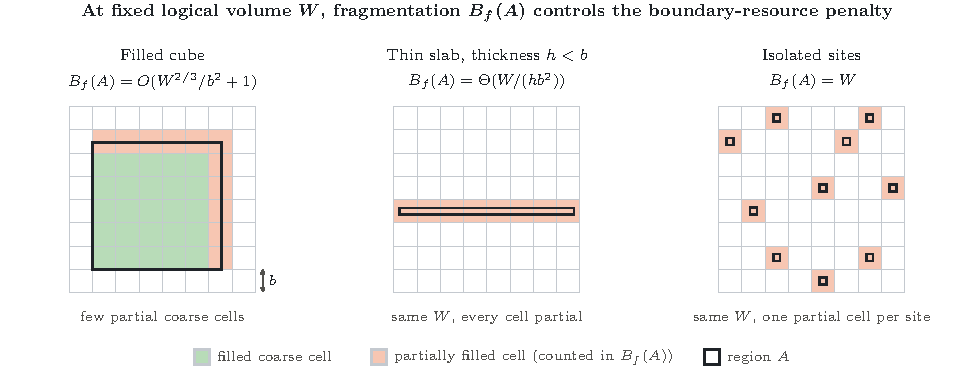
\includegraphics[width=0.92\textwidth]{fragmentation_Bf.pdf}
\caption{Qualitative role of the coarse fragmentation term $B_f(A)$ at fixed logical volume $W$, with coarse boxes of side $b=\Theta(f^{1/6})$.  A filled bounded-aspect cube has $B_f(A)=O(W^{2/3}/b^2+1)$, so the partial-cell term $f^{3/2}B_f$ is subleading once $W\gtrsim\sqrt f$.  A thin slab of thickness $h<b$ has $B_f(A)=\Theta(W/(hb^2))$ and a partial-cell cost $\Theta(Wf^{7/6}/h)$, which exceeds the extensive $Wf$ term.  Isolated sites at mutual spacing at least $b$ give $B_f(A)=W$ and cost $\Theta(Wf^{3/2})$.  These terms enter the space bound $O\!\bigl(Wf+(B_f(A)+1)f^{3/2}\bigr)$ of Theorem~\ref{thm:A24}/Eq.~(A26).}
\label{fig:fragmentation}
\end{figure*}

\begin{corollary}[Bounded-aspect specialization]
\label{cor:bounded-aspect-packing}
If $A$ is a connected bounded-aspect three-dimensional grid box, then at the
packing scale above
\begin{equation*}
 B_b(A)=O\!\left((W/K)^{2/3}+1\right),
\end{equation*}
and the number of data/factory cells is $O(W/K+1)$.
\end{corollary}
\begin{proof}
Only coarse boxes intersecting the $O(1)$ outer faces can be partial.  For a
bounded-aspect box the number of such boxes is at most a constant times its
coarse surface area, $O((W/b^3)^{2/3}+1)$.  Since $b^3=\Theta(K)$ this is the
stated bound.  When $W\ge K$, $(W/K)^{2/3}\le W/K$; when $W<K$ the additive
one dominates.
\end{proof}

\paragraph{Constant and ceiling ledger.}
The constants $\beta_0$ (static gauging), $c_1$ (circuit-to-phenomenological
spread), $\alpha$ (composed circuit distance), $\gamma$ (earliest-stage courier
charge), $C_0$ (stage volume), $\kappa$ (resource-boundary linking),
$C_{\rm dist}$ (distillation pairs), $p_\star$ (cluster counting), and the
chosen $p_{\rm th}$ depend only on the fixed input
family constants, finite local cell/template catalog, and fixed scheduling
conventions.  They are independent of $W,T,N,f$ and of the realized adaptive
branch.  Ceilings change the displayed distance and padding inequalities only
by additive $O(1)$ terms, which are absorbed by $f_{\min}$.  The physical raw
stage remains separate with $s_{\rm raw}\ge1$ and is never assigned encoded
distance.

\paragraph{Informal corollary (connected bounded-aspect regions).}
\label{par:informal-resource}
For a connected bounded-aspect logical region $A$, Corollary~\ref{cor:bounded-aspect-packing}
reduces the cell count to $O(W/K+1)$.  Below threshold at target failure
$\varepsilon$, with $f=\Theta(\log(WT/\varepsilon))$ at fixed
$p<p_{\mathrm{th}}$, universal nearest-neighbor computation therefore uses
roughly
\begin{equation*}
 O\bigl(Wf+f^{3/2}\bigr)
\end{equation*}
physical qubits, together with the polylogarithmic depth factor $\Psi$ of
(A27).  The fully general fragmentation-aware resource theorem is stated next.

\paragraph{Dependency map.}
Figure~\ref{fig:ft-dependency} separates the theorem chain from cited inputs and finite supporting checks.

\begin{figure*}[t]
\centering
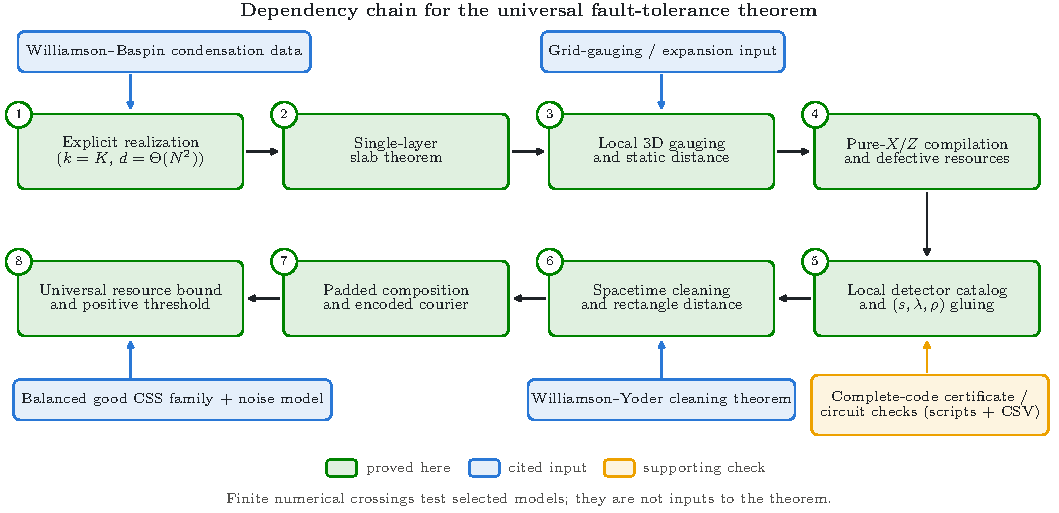
\includegraphics[width=\textwidth]{ft_proof_dependency.pdf}
\caption{Dependency map for the universal fault-tolerance theorem. Green boxes form the proof chain, blue boxes are cited inputs, and amber boxes are finite supporting checks.  The supporting checks and numerical crossings are not hypotheses of Theorem~\ref{thm:A24}.}
\label{fig:ft-dependency}
\end{figure*}

\begin{theorem}[Universal fault-tolerant resource theorem]\label{thm:A24}
Use the fixed-degree Quantum Tanner family of Lemma~\ref{lem:tanner-dense}, or more generally any balanced good CSS family with boundedly dense sizes, and apply the explicit layer-code realization of Sec.~\ref{sec:explicit-realization} to it, using the slab representatives of
Theorem~\ref{thm:slab-resolved} and the distance bound of Theorem~\ref{thm:explicit-distance}.  Use the explicit resource-coordinate
convention of Lemma~\ref{lem:A5} and Tables~\ref{tab:steane-map} and~\ref{tab:rm-map}, together
with the canonical extraction schedule and encoded courier of
Theorem~\ref{thm:A16}.  Under the local-stochastic Pauli noise model (A1),
there are constants $p_{\mathrm{th}},c,f_{\min}>0$ such that, for
$0<p<p_{\mathrm{th}}$, a nearest-neighbor three-dimensional logical circuit
whose finite allocated region is $A\subset\mathbb Z^3$, with $W=|A|$, depth
$T$, and target error $0<\varepsilon<1/2$ can be simulated with
\begin{equation}
 f=\max\left\{f_{\min},
 \left\lceil\frac{c\log(WT/\varepsilon)}{\log(p_{\mathrm{th}}/p)}\right\rceil
 \right\}.                                                         \tag{A25}
\end{equation}
Let $K=\Theta(\sqrt f)$ be the number of logicals in the selected
layer-code cell, choose $b=b(f)=\Theta(K^{1/3})=\Theta(f^{1/6})$ as in
Lemma~\ref{lem:architecture-packing}, and abbreviate
$B_f(A):=B_{b(f)}(A)$.  The simulation uses
\begin{equation}
 O\!\left(Wf+(B_f(A)+1)f^{3/2}\right)                             \tag{A26}
\end{equation}
physical qubits and depth
\begin{equation}
 O(Tf^{3/2}\Psi),\qquad
 \Psi=O(15^\ell)=O\bigl(f^{\log_215}\bigr),              \tag{A27}
\end{equation}
where the number $\ell$ of distillation levels obeys
$2^\ell=O(\min\{f,\log(WT/\varepsilon)\})$.  Thus the depth is
$O(Tf^{3/2+\log_215})\subseteq O(Tf^{5.41})$ for the minimal-space factory
schedule.
Every persistent data logical is stored in a layer-code block.  Reserved gate
ancillas and live factory resources are included in the physical-space count.
\end{theorem}
\begin{proof}
Fix the edge multiplicity $m_0$ of Theorem~\ref{thm:local-gauging}, so that
$\beta_0=1$; any other fixed multiplicity changes only constants.  Choose the
input size so that $\beta_0d\ge f/\alpha$.  By
Theorem~\ref{thm:A16} the resource boundaries have linking
$\rho\geq\kappa R$ for fixed $\kappa>0$.  Define
\begin{equation*}
 C_R:=\max\{1,1/\alpha,1/\kappa\},\qquad
 R=R_{\mathrm{pad}}=\lceil C_R f\rceil .
\end{equation*}
Then $\alpha\min\{\beta_0d,R\}\ge f$ and $\kappa R\ge f$
exactly; finite endpoint offsets are absorbed in the already fixed
$f_{\min}$.
  Lemma~\ref{lem:tanner-dense} supplies bounded density for the
Quantum Tanner input family (or use the assumed bound for a general family),
giving $N=\Theta(\sqrt f)$, $K=\Theta(\sqrt f)$, and
$n=\Theta(f^{3/2})$.  Lemma~\ref{lem:architecture-packing} gives
$O(W/K+B_f(A)+1)$ data/factory cells and makes the fixed-separation two-cell
requirement explicit.  Multiplying by the cell volume $n=\Theta(f^{3/2})$
gives (A26), since $(W/K)f^{3/2}=\Theta(Wf)$.  Each factory's live courier uses only
a constant number of additional blocks at any one time; these occupy the
factory/courier reserve positions of the supercells of
Lemma~\ref{lem:architecture-packing} and are already included in the cell count.

Apply Theorem~\ref{thm:A11}, (A20), and the defective-resource lemmas.
Conditional on the large-cluster complement, the injected resources form a
local-stochastic defective family (Definition~\ref{def:defective-family})
with parameter $q_0\le C_{\rm inj}\sqrt p$ after enlarging the fixed constant
if necessary, and (A8) makes the final resource error at most
$\varepsilon/(2c_{\rm res}WT)$ after the stated number of levels, where
$c_{\rm res}=O(1)$ bounds the number of final resources consumed per logical
site and layer.  The complete
fixed skeleton, including factory and courier locations, has
$M\leq C_MWT\Psi f^{a_M}$ mechanisms for fixed $C_M,a_M$.  Put
$X=WT/\varepsilon$, $L=\log(p_{\mathrm{th}}/p)$, and
$\delta=\log(p_\star/p_{\mathrm{th}})\geq\log2$.  Then
\begin{equation}
 (p/p_\star)^{f/4}=\exp[-f(L+\delta)/4].                            \tag{A28}
\end{equation}
If the second term in (A25) determines $f$, the factor $e^{-fL/4}$
is at most $X^{-c/4}$.  If instead $f=f_{\min}$, then
$c\log X/L\leq f_{\min}$, so again $e^{-fL/4}\leq X^{-c/4}$.
The remaining $f^{a_M} e^{-\delta f/4}$ is uniformly bounded for
$f\geq f_{\min}$, and $\Psi=(\log X)^{O(1)}$.  Choosing $c$ larger than
the fixed polynomial exponents therefore makes (A12) at most
$\varepsilon/2$, uniformly for every $0<p<p_{\mathrm{th}}$.  A union bound over
consumed final resources completes the correctness proof.

The recurrence may be stopped at the least $\ell$ satisfying
$2^\ell\log(1/(C_{\rm dist}q_0))\geq c'\log X$ for a fixed $c'$.
Because $q_0\leq C_{\rm inj}\sqrt p$ and (A23) gives
$C_{\rm dist}C_{\rm inj}\leq1/(4\sqrt{p_{\rm th}})$, we have
$C_{\rm dist}q_0\leq\tfrac14\sqrt{p/p_{\rm th}}$ and hence
$\log(1/(C_{\rm dist}q_0))\geq\log4+L/2$.  Minimality of $\ell$
therefore gives $2^\ell\leq 2c'\log X/(\log4+L/2)$.  This is $O(\log X)$,
and since (A25) gives $\log X\leq fL/c$ it is also at most $4c'f/c=O(f)$,
including the regime $f=f_{\min}$.  Consequently
$\ell\leq\log_2f+O(1)$ and
$\Psi=O(15^\ell)=O((2^\ell)^{\log_215})=O(f^{\log_215})$, with
$\log_215\approx3.907$.  A depth-first factory schedule
stores only $O(\ell)$ completed candidate resources at once (with a constant
factor for the branching protocol), which fits among $K=\Theta(\sqrt f)$
factory logicals after increasing $f_{\min}$.  One distilled resource uses $O(\Psi)$ serialized gadget slots, each of
$O(f)$ rounds, hence costs $O(f\Psi)$ rounds.  A logical layer requires
$O(K)$ resources per data block; producing the batch costs
$O(Kf\Psi)=O(f^{3/2}\Psi)$ rounds, proving (A27).  This serial,
depth-first schedule is chosen to keep the space bound (A26); running several
factories in parallel per data block would shorten the depth at the cost of
additional factory cells.
\end{proof}

For a connected bounded-aspect allocated box,
Corollary~\ref{cor:bounded-aspect-packing} gives
$B_f(A)=O((W/\sqrt f)^{2/3}+1)$.  If $W\ge\sqrt f$, its contribution
$f^{3/2}B_f(A)=O(W^{2/3}f^{7/6}+f^{3/2})$ is $O(Wf+f^{3/2})$; if
$W<\sqrt f$, one-cell/additive terms dominate.  Thus the previous compact
space bound $O(Wf+f^{3/2})$ is recovered in the bounded-aspect regime, while
(A26) quantifies the extra cost of thin, holed, or fragmented regions.

\begin{corollary}[Transfer to uniformly slab-supported 3D CSS families]
\label{cor:slab-transfer}
The layer-code origin of the slabs is not used after
Theorem~\ref{thm:slab-resolved}.  Let $\{\mathcal C_N\}$ instead be any
three-dimensional local CSS family satisfying all of the following uniformly:
(i) an embedding in a fixed finite-type three-dimensional lattice with bounded
qubit/check density, check weight, check degree, and stabilizer diameter;
(ii) physical block aspect ratio $O(1)$;
(iii) parameters $n=\Theta(N^3)$, $K=\Theta(N)$, and
$d_X,d_Z=\Theta(N^2)$; (iv) boundedly dense available values of $N$; and
(v) fixed coordinate axes such that every pure $X$ logical class and every
pure $Z$ logical class has a representative supported in at most $t_0=O(1)$
parallel coordinate planes of the appropriate orientation.  Then the local
gauging, detector, spacetime-composition, courier, and threshold arguments of
Secs.~\ref{sec:gauging}--\ref{sec:ft} apply verbatim, and Theorem~\ref{thm:A24} holds for this family
with the same asymptotic bounds, including the fragmentation term in (A26).
\end{corollary}
\begin{proof}
The layer-code defect network is used in the architecture proof only to
establish the uniform slab representatives and the parameter scaling.  Under
assumptions (i)--(v), those inputs are supplied directly.
Corollary~\ref{cor:cubic-box-relative-expansion} and
Lemma~\ref{lem:reserved-ports} give constant relative expansion
after the same constant refinement;
Theorem~\ref{thm:local-gauging} then gives constant-factor deformed
distance and bounded local incidence.  The finite-radius extraction and
detector-template arguments of Proposition~\ref{prop:nn-extraction} and
Proposition~\ref{prop:uniform-local-detectors} use only those uniform locality
bounds.  Boundary gluing, relative cleaning, padded composition, and the
courier lemmas are code-family agnostic once the static space-distance and
local-template hypotheses hold.  Finally $n=\Theta(N^3)$,
$K=\Theta(N)$, $d=\Theta(N^2)$ and boundedly dense sizes reproduce
$N=\Theta(\sqrt f)$ and the resource accounting in
Theorem~\ref{thm:A24}.
\end{proof}

For very small $p$, scaling statements should use
$\max\{1,\log(WT/\varepsilon)/\log(1/p)\}$; otherwise a displayed qubit count
would incorrectly tend to zero.  Finally, the extensive lower bound
$\Omega(Wf)$ matches (A26) only when $W=\Omega(\sqrt f)$, so that the additive
one-block term does not dominate.  The occupancy condition
$k=O(\sqrt f)$ alone does not establish constant-factor optimality in the
small-$W$ regime.



\section{Storage benchmark}\label{app:storage-details}
\subsection{Statement and scope}\label{sec:lower}
Related volume limits on quantum storage appear in Ref.~\cite{FlammiaStorage}.
For comparison only, consider fully occupied unknown-data blocks stored through
independent depolarizing noise with $0<p\leq3/4$, target infidelity
$0<\varepsilon\leq1/2$, and maximally entangled logical inputs.  Put
$q=p(1-p)/3$.  The reference-system Pauli-twirl argument below gives
\begin{equation}
 F_e\leq\prod_{b=1}^{B}\bigl(1-q^{\lceil d_b/2\rceil}\bigr),
 \label{eq:exact-storage}
\end{equation}
and therefore, whenever $F_e\geq1-\varepsilon$,
\begin{equation}
 \sum_b q^{\lceil d_b/2\rceil}\leq-\log(1-\varepsilon)\leq2\varepsilon.
 \label{eq:sum-storage}
\end{equation}
For equal $[[n,k,d]]$ blocks with $B=W/k$, this implies
$d\geq2\log(W/(2k\varepsilon))/\log(1/q)-2$.  A valid nonnegative distance
for the Bravyi--Poulin--Terhal (BPT) inequality $kd^{2/(D-1)}\le c_Dn$ in $D$
dimensions is
\begin{equation}
 d_* = \max\left\{1,\;2\left\lceil\frac{\log(1/(2\varepsilon))}{\log(1/q)}\right\rceil-1\right\},
 \label{eq:distance-floor}
\end{equation}
so a valid nonuniform volume benchmark is
\begin{equation}
 \sum_b n_b\geq \frac{W}{c_D}\,d_*^{\,2/(D-1)}.
 \label{eq:storage-volume}
\end{equation}
This comparison keeps $k$ inside
$\log(W/(k\varepsilon))$ and does not yield a uniform
$\log(W/\varepsilon)$ bound over arbitrary occupancies.  Matching to the
upper space bound is claimed only in the stated comparable regime, including
$W=\Omega(\sqrt f)$; reserved gate/factory ancillas are not counted as stored
unknown data in the same $W$.



The proof of Eqs.~\eqref{eq:exact-storage}--\eqref{eq:storage-volume} follows.

\begin{proof}
Choose a minimum-weight nonidentity logical Pauli $L_b$ in block $b$, split its support into sets of sizes $a_b=\lceil d_b/2\rceil$ and $d_b-a_b$, and let $E_1,E_2$ be the restrictions of $L_b$ to those sets. For each Pauli $F$ outside this support, the independent depolarizing channel assigns probabilities
\begin{align}
 P_1(F)&=(p/3)^{a_b}(1-p)^{d_b-a_b}\Pr(F),\\
 P_2(F)&=(p/3)^{d_b-a_b}(1-p)^{a_b}\Pr(F).
\end{align}
Set $m_F=\min(P_1(F),P_2(F))$ and $M_b=\sum_F m_F$. Since $p/3\leq1-p$,
\begin{equation}
 M_b=(p/3)^{a_b}(1-p)^{d_b-a_b}\geq q^{a_b}.
\end{equation}
Pairing these two errors decomposes the block channel into a component of weight $2M_b$ of the form $\mathcal N_b\circ\mathcal D_{L_b}$ and a remaining channel, where
\begin{equation}
 \mathcal D_{L_b}(\rho)=\tfrac12(\rho+L_b\rho L_b^\dagger)
\end{equation}
and $\mathcal N_b$ is a mixture of the errors $E_1F$. On half of a maximally entangled logical state, $\mathcal D_{L_b}$ can equivalently act by $L_b^T$ on the reference. It then commutes with every subsequent operation on the physical system.

Expand the product of block channels and let $S$ be the subset of blocks selecting the twirled component. The $|S|$ independent reference Paulis map the maximally entangled target projector to $2^{|S|}$ orthogonal rank-one projectors with equal weights. The pinched target therefore has operator norm $2^{-|S|}$. The conditional output fidelity, even after an arbitrary joint recovery, is at most that norm. Averaging gives
\begin{equation}
 F_e\leq\mathbb E_S 2^{-|S|}=\prod_b(1-M_b)\leq\prod_b(1-q^{a_b}).
\end{equation}
Taking logarithms and using $-\log(1-x)\geq x$ proves Eq.~\eqref{eq:sum-storage}. Inverting $q^{\lceil d/2\rceil}\leq u$ requires $\lceil d/2\rceil\geq\lceil\log(1/u)/\log(1/q)\rceil$, hence $d\geq2\lceil\log(1/u)/\log(1/q)\rceil-1$. This yields Eq.~\eqref{eq:distance-floor}; the BPT tradeoff then gives the volume bound.
\end{proof}

\paragraph{Median-distance consequence.}
Put $a=\log(B/(4\varepsilon))/\log(1/q)$. Fewer than half the blocks satisfy
\begin{equation}
 d_b<2\lceil a\rceil-1.
 \label{eq:median}
\end{equation}
Indeed, this inequality implies $\lceil d_b/2\rceil<a$, so $q^{\lceil d_b/2\rceil}>4\varepsilon/B$; summing proves the count. The ceiling is essential. For example, one unencoded qubit with $B=n=k=d=1$ and $\varepsilon=p=0.01$ has $q=0.0033$ and $2a\simeq1.12670$; the integer cutoff in Eq.~\eqref{eq:median} is instead $1$.

\paragraph{Scope of the benchmark.}
The comparison keeps $k$ inside $\log(W/(k\varepsilon))$. It does not imply a lower bound with $\log(W/\varepsilon)$ uniformly over arbitrary occupancies. For the bounded-aspect logical regions in which the architecture upper bound reduces to $O(Wf+f^{3/2})$, the $W<\sqrt f$ regime is dominated by one layer-code block; Eq.~\eqref{eq:storage-volume} supplies only a bound of order $Wf$ in the comparable logarithmic regime. Thus constant-factor matching to this lower bound is restricted to $W=\Omega(\sqrt f)$ as well as the stated occupancy, depth, geometry, and noise restrictions; irregular regions additionally incur the fragmentation term in (A26).

The storage benchmark applies to fully occupied unknown-data blocks. Reserved logical qubits used for known gate ancillas or factory states are not counted as stored unknown data in the same $W$; computational-space comparisons must therefore account for working logical capacity separately.



\section{Reusable boundary-state composition theorem}
\label{app:abstract-composition}
The complete-circuit proof uses the schedule-specific restriction lemma, Lemma~\ref{lem:rectangle-restriction}.  We record its abstract connected-component form here for reuse; this section introduces no additional hypothesis into Theorem~\ref{thm:A24}.

\begin{proposition}[Canonical rectangle restriction]
\label{prop:canonical-rectangle-restriction}
For every realized causal branch of the canonical finite slot catalog, the
global detector/effect matrix satisfies the rectangle restriction property:
if a connected detector-trivial component meets at most one active primitive,
then its restriction to a surrounding padded subchain is a valid relative
rectangle solution with the inherited boundary syndrome, last-round
records, and logical frame left arbitrary, and with exactly the same
protected relative effect.
\end{proposition}
\begin{proof}
This is Lemma~\ref{lem:rectangle-restriction}.  The required physical rows are
the uniformly local rows of $D^{\mathrm{loc}}$ from
Proposition~\ref{prop:uniform-local-detectors}; Proposition~\ref{prop:local-suffices}
and Lemma~\ref{lem:canonical-gluing} show that complete boundary variables
suffice to glue and restrict them.  The full space
$\mathcal R_g^{\mathrm{full}}$ is only the algebraic closure used to audit boundary
relations, so no nonlocal left-kernel basis is inserted into the fault graph
and no perfect-cut assumption is introduced.
\end{proof}

\begin{theorem}[Abstract padded connected-component composition]
\label{thm:abstract-padded-composition}
Consider any linear phenomenological detector model with bounded temporal
fault-graph range $\tau$.  Suppose successive active rectangles sharing
support are separated by $R_{\mathrm{pad}}$ idle rounds, every connected component
meeting at most one active rectangle has a valid relative restriction with
its protected effect preserved, protected active rectangles have relative
fault distances $\delta_g^{\mathrm{rel}}$, and idle rectangles have relative fault
distance $\delta_{\mathrm{mem}}^{\mathrm{rel}}$.  Then
\begin{equation}
 f_{\mathrm{ph}}\geq
 \min\left\{
   \min_g\delta_g^{\mathrm{rel}},\ \delta_{\mathrm{mem}}^{\mathrm{rel}},\
   1+\left\lfloor\frac{R_{\mathrm{pad}}-\tau}{\tau}\right\rfloor
 \right\}.                                                        \label{eq:composed-distance}
\end{equation}
If the detector/effect vector of every circuit mechanism is the sum of the
vectors of at most $c_1$ phenomenological mechanisms, then
\begin{equation}
 f_{\mathrm{circ}}\geq\left\lceil f_{\mathrm{ph}}/c_1\right\rceil.           \label{eq:circuit-distance}
\end{equation}
\end{theorem}
\begin{proof}
Take a detector-trivial pattern with nonzero protected effect.  By
Lemma~\ref{lem:componentwise}, one of its connected components $C$ is
itself detector trivial and has nonzero protected contribution.  If $C$ is
smaller than the third term, its temporal span is below $R_{\mathrm{pad}}$ and it
meets at most one active rectangle.  The assumed relative restriction then
places it in one active or idle rectangle without changing its protected
relative effect, so its size is at least the corresponding local relative
distance.  Otherwise its size is already at least the padding term.  The
circuit-level statement follows by replacing each circuit mechanism by its
bounded phenomenological image; connectivity of that image is not required.
\end{proof}

For the canonical schedule, Proposition~\ref{prop:canonical-rectangle-restriction} and Lemma~\ref{lem:relative-rectangle-distance} verify the hypotheses of
Theorem~\ref{thm:abstract-padded-composition}, and Eq.~\eqref{eq:composed-distance}
is exactly the protected composition input used in Theorem~\ref{thm:A16}.
The raw resource boundary lies outside the ordinary protected class and is handled by Lemma~\ref{lem:raw-quotient-distance}; encoded courier
changes are handled by Lemmas~\ref{lem:encoded-courier-distance} and~\ref{lem:earliest-stage-charging}.



\section{Reproducibility package}\label{sec:repro}

The submission includes \texttt{reproducibility\_checks.py}, \texttt{glue\_example\_check.py}, and \texttt{operational\_anchor.py}.  Running
\begin{equation*}
\texttt{python reproducibility\_checks.py}
\end{equation*}
checks the slab-cell boundary matrices derived below from the published condensation generators, including the $110$ pass-through and their $X\leftrightarrow Z$ duals.  It also tests all even prefix-parity words of lengths $2$ to $8$, longer deterministic stress words, and the GF(2) support-rank formula used by the slab criterion.  For the logical and detector layers it checks the seven- and fifteen-qubit single-$Z$ syndrome maps; the $S$, $T$, $S_X$, and CNOT Kraus identities; T0--T7 detector matrices; boundary-state and gluing identities; one-bit teleportation and Pauli transport; and $SS_XS=e^{i\pi/4}H$ up to global phase.  Finally, it propagates single-location Paulis through the T8 master words for support weights $1$--$8$ and shuttle lengths $0$--$2$, transcribes the WB Sec.~VI~B items 3--8 junction supports in unit-cubic edge coordinates, checks the two surface-code subdivision identities, and checks the Steane and punctured Reed--Muller transversal phase orientations.

The scripts write \nolinkurl{factory_map_audit.csv}, \nolinkurl{t8_single_fault_audit.csv}, \nolinkurl{t8_master_routing_catalog.csv}, \nolinkurl{slab_cell_audit.csv}, \nolinkurl{wb_junction_support_catalog.csv}, and \nolinkurl{refinement_move_audit.csv}.  The matrix comparisons use tolerance $10^{-12}$.  The package includes a pinned \nolinkurl{requirements.txt} and \nolinkurl{environment-known-good.json}; the latter records the Python and package versions used for the archived numerical campaign.

The slab-cell calculation derives $H_{\rm end}=[1\;1]$ and $H_{\rm mid}=[1\;1\;1]$ (kernels $\{00,11\}$ and $\{000,110,101,011\}$, including the $110$ pass-through) from the published condensation generators.

\paragraph{Construction, distance, composition, and resource scripts.}
\texttt{layer\_code\_explicit.py} generates the complete check matrices of the
explicit realization (and of the single-chart transcription, as a negative
control) for any CSS input.  \texttt{slab\_gluing\_certificate.py} runs the
certificate of Sec.~\ref{sec:certificate} and writes
\nolinkurl{slab_cert_A_archived_all_words.csv},
\nolinkurl{slab_cert_A_archived_full_syndrome.csv},
\nolinkurl{slab_cert_B_complete_codes.csv}, \nolinkurl{slab_cert_C_forms.csv},
\nolinkurl{slab_cert_D_exhaustive_words.csv}, and
\nolinkurl{slab_cert_E_wall_controls.csv}; two instances are exported with all
check and qubit labels (\nolinkurl{explicit_layer_code_422_s2.npz},
\nolinkurl{explicit_layer_code_steane_s2.npz}).
\texttt{explicit\_layer\_code\_distance.py} computes the distances of
Table~\ref{tab:explicit-distance} with the CP-SAT solver wrapped in
\texttt{min\_weight\_logical.py}.  \texttt{distance\_lower\_bound\_check.py}
checks the plane-restriction and shortest-side steps of
Theorem~\ref{thm:explicit-distance} and compares its bound with these
distances (\nolinkurl{distance_lower_bound_check.csv},
\nolinkurl{distance_bound_vs_exact.csv}).  \texttt{frame\_propagation\_check.py}
checks the syndrome terms of (A15b) and the contained-component lemma;
\texttt{glue\_example\_check.py} checks the record-aware worked example; and
\texttt{boundary\_composition\_check.py} compares the direct and composed
detector/effect maps on explicit blocks
(\nolinkurl{boundary_composition_check.csv}).
\texttt{resource\_defect\_check.py} checks the defective-resource lemmas, the
single-defect exactness of both factories, and the malignant-pattern counts
(\nolinkurl{resource_defect_check.csv}).  \texttt{two\_block\_measurement.py}
builds and analyzes the circuits of Sec.~\ref{sec:two-block}, with recorded
integer seeds (\texttt{tighten\_two\_block.py} reruns selected solves with a
longer time limit); \texttt{resource\_estimate.py} produces the estimate of
Sec.~\ref{sec:resource-estimate}; and \texttt{make\_junction\_figure.py} draws
Fig.~\ref{fig:junction-geometry} from a generated instance.  These scripts need
NumPy, SciPy, Stim, ldpc (GF(2) rank and BP+LSD decoding), OR-Tools, and
Matplotlib, pinned in \nolinkurl{requirements-revision.txt} and installed with
\texttt{pip install -r requirements-revision.txt}.  The exact commands and the
time limits of the CP-SAT runs are listed in \nolinkurl{REVISION_RUNS.md}.

The archived scripts \texttt{wb\_microscopic\_\allowbreak bridge\_audit.py},
\texttt{wb\_exact\_cell\_\allowbreak patch\_audit.py}, and
\texttt{wb\_layer\_code\_\allowbreak instance.py}
are retained for provenance; Sec.~\ref{sec:finite-cell-cert} explains why their
certificates are superseded.

\paragraph{Operational-anchor files.}
Running \texttt{python operational\_anchor.py} regenerates: (i) the incidence values $r_{\mathrm{inc}}^{(\infty)}=1$, $r_{\mathrm{inc}}^{(G)}=2$, and maximum support weight $6$ from \texttt{wb\_junction\_support\_catalog.csv}; (ii) \texttt{finite\_instance\_slab\_certificate.csv} for a stacked $4\times4$ toric CSS code ($n=96$, $k=6$), with minimum passing thickness $t_{\min}=3$; (iii) \texttt{phenomenological\_mw\_demo.csv} for distance-$3$ and $5$ toric codes; and (iv) \texttt{operational\_constants.csv}.  The complete script sequence is listed in \texttt{run\_verification.sh}.

\section{Canonical schedule, local detectors, and boundary-state gluing}\label{sec:catalog}

For each primitive $g$, the physical decoder uses a uniformly local detector catalog $D_g^{\mathrm{loc}}$.  The complete stabilizer transition space $\mathcal R_g^{\mathrm{full}}$ is a separate algebraic closure for boundary-state consistency.  Its elements are not automatically physical detector rows and are not inserted into the fault graph merely because they belong to a left kernel.

\subsection{Binary Pauli boundary coordinates}
Represent an $n$-qubit Pauli, modulo phase, by a binary symplectic vector
$p=(x\mid z)\in\mathbb F_2^{2n}$.  Let $J$ denote the standard symplectic
form.  At every cut choose an independent stabilizer generator matrix
$H\in\mathbb F_2^{r\times 2n}$ and a complete symplectic logical basis.  The
boundary syndrome is
\begin{equation}
 s=HJp^T,
 \tag{S1}
\end{equation}
and the logical-frame vector $\lambda$ is the vector of commutators of $p$
with the chosen logical partners.  The map $p\mapsto(s,\lambda)$ has kernel
exactly the stabilizer row space.  Thus $(s,\lambda)$ is a complete coordinate
for the Pauli class modulo stabilizers; an inherited error at a fault-free cut
need not have $s=0$.  The classical boundary datum is the vector $\rho$ of
reported-record deviations of the last round before the cut,
$\rho=\Pi s+\mu_\partial$, where $\Pi$ gives the syndrome of each measured
check through the generators and $\mu_\partial$ are the record flips of that
round (Eq.~(A15-rec)).  A cut carries $(s,\lambda,\rho)$.

For each primitive $g$, let $e_g$ denote its phenomenological fault bits and
$\delta_g$ the values of its detector rows, including the rows that straddle
its input cut.  The physical local detector/effect system has the form
\begin{align}
 \delta_g&=D_g^{\mathrm{loc}}e_g+A_g^{\mathrm{loc}}s_g^{\rm in}
 +P_g^{\mathrm{loc}}\rho_g^{\rm in},\tag{S2}\\
 \lambda_g^{\rm out}&=L_g\lambda_g^{\rm in}+C_gs_g^{\rm in}+E_ge_g,\tag{S3}\\
 o_g&=Q_g\lambda_g^{\rm in}+G_gs_g^{\rm in}+F_ge_g,\tag{S4}
\end{align}
with the output variables of (A15a$'$).  Here $o_g$ contains any committed
protected effect of the slot, and a pattern is detector-trivial when every
$\delta_g$ vanishes.  The syndrome terms $C_g$, $G_g$ record how the
representatives chosen at the two cuts differ by stabilizers (see the
discussion of (A15b)); they vanish in the idle example below, where both cuts
use the same representatives.

\subsection{Uniformly local physical detector catalog}
The local rows are generated from the following finite set of \emph{master
templates}.  A block-size-dependent row is obtained only by translating one
of these templates to one of the finitely many labeled local geometries of
the refined lattice.  Consequently there are constants
$r_{\rm det},a_{\rm det},b_{\rm det}=O(1)$ such that every row is contained in
a radius-$r_{\rm det}$ spacetime ball, every row touches at most
$a_{\rm det}$ phenomenological mechanisms, and every mechanism touches at
most $b_{\rm det}$ rows.  These bounds arise from the finite template types,
not from the dimension of a block-size-dependent relation space.

Write $m_t(C)\in\mathbb F_2$ for a flip of the reported eigenvalue of a
measured Pauli check $C$ at the indicated half-integer measurement time.  If
$E$ is the net phenomenological Pauli mechanism in a bounded interval, write
$\chi_C(E)=1$ when $E$ anticommutes with $C$ after propagation to the relevant
slice.  For an edge ancilla, $\iota_e$ denotes a wrong $Z_e$ eigenvalue at
$|0\rangle$ preparation and $\nu_e$ a flipped final $Z_e$ readout.  All sums
below are over $\mathbb F_2$.  The $X\leftrightarrow Z$ dual templates are
understood wherever the opposite CSS type is extracted.

\paragraph{T0: consecutive measurement of one persistent check.}
For any check $C$ measured in two consecutive rounds,
\begin{align}
 d_C^t&=m_{t-1/2}(C)+m_{t+1/2}(C)+\chi_C(E_t)=0,
 \tag{T0a}\\
 D_C^t&=[\,1\;1\mid\chi_C\,].
 \tag{T0b}
\end{align}
This is the only temporal template in an idle window and is also used for
$A_v$, $B_p$, and $\widetilde s_j$ during repeated gauged rounds.

\paragraph{T1: bounded same-slice dependency.}
If a bounded local set of simultaneously measured checks obeys
$C_1\cdots C_r=I$ (including the known sign convention), then
\begin{equation}
 d_{\rm dep}^t=\sum_{i=1}^r m_t(C_i)=0,
 \qquad D_{\rm dep}^t=[\,1\;1\;\cdots\;1\,].
 \tag{T1}
\end{equation}
The number $r$ is uniformly bounded.  These are the optional space-only
meta-check rows mentioned in the spacetime-code construction; adding them can
only further restrict the detector-trivial set.

\paragraph{T2: bounded merge/split relation.}
Suppose a local transition has input checks $A_1,\ldots,A_r$ and output checks
$B_1,\ldots,B_s$ whose Pauli products agree on the common boundary,
$\prod_iA_i=\prod_jB_j=:C$.  The physical transition row is
\begin{align}
 d_{A\to B}&=\sum_i m_-(A_i)+\sum_j m_+(B_j)
   +\chi_C(E_\partial)=0,
 \tag{T2a}\\
 D_{A\to B}&=[\,\mathbf1_r\;\mathbf1_s\mid\chi_C\,].
 \tag{T2b}
\end{align}
Only relations supported inside one bounded transition cell are instantiated.
T0 is the special case $r=s=1$ with no change of check type.

\paragraph{T3: explicit gauging-entry rows.}
Let the modified check be
$\widetilde s_j=s_j\prod_{e\in\mu_j}Z_e$, where the pairing path $\mu_j$ has
uniformly bounded length, and let $p$ be a unit-square cycle.  At the first
deformed round the two endpoint rows are
\begin{align}
 d_{\widetilde s_j}^{\rm in}
 &=m_-(s_j)+m_+(\widetilde s_j)
   +\sum_{e\in\mu_j}\iota_e+\chi_{\widetilde s_j}(E_{\rm in})=0,
 \tag{T3a}\\
 d_{B_p}^{\rm in}
 &=m_+(B_p)+\sum_{e\in p}\iota_e+\chi_{B_p}(E_{\rm in})=0.
 \tag{T3b}
\end{align}
There is no additional macroscopic entry row for the product of all $A_v$
outcomes: that product is the committed logical-measurement effect.  The
$A_v$ records use T0 once a second deformed round exists; their open temporal
endpoint is exactly the endpoint used in the timelike-distance argument.

\paragraph{T4: explicit gauging-exit rows.}
At the return to the undeformed code,
\begin{align}
 d_{\widetilde s_j}^{\rm out}
 &=m_-(\widetilde s_j)+m_+(s_j)
   +\sum_{e\in\mu_j}\nu_e+\chi_{s_j}(E_{\rm out})=0,
 \tag{T4a}\\
 d_{B_p}^{\rm out}
 &=m_-(B_p)+\sum_{e\in p}\nu_e+\chi_{B_p}(E_{\rm out})=0.
 \tag{T4b}
\end{align}
Together T3, T0 on the repeated deformed checks, and T4 are the local detector
generators listed for gauging measurement in the Williamson--Yoder gauging construction~\cite{WilliamsonYoderGauging};
T1 is added when the code has bounded local relations.

\paragraph{T5: product-state birth and terminal readout.}
For a bounded-support $Z$ check $C=\prod_{q\in S}Z_q$ following $|0\rangle$
preparation, and for the dual terminal $Z$ readout of the same support,
\begin{align}
 d_C^{\rm birth}&=m_+(C)+\sum_{q\in S}\iota_q+\chi_C(E_{\rm birth})=0,
 \tag{T5a}\\
 d_C^{\rm death}&=m_-(C)+\sum_{q\in S}\nu_q+\chi_C(E_{\rm death})=0.
 \tag{T5b}
\end{align}
The $X$-basis versions are identical after exchanging $X$ and $Z$.  Encoded
$|0\rangle/|+\rangle$ birth, protected logical readout, and encoded discard
are tiled by T0--T2 and these endpoint rows.

\paragraph{T6: raw injection, courier, and factory slots.}
These introduce no new detector-row species.  The protected
$Z_qZ_{B_0}$ or $Z_{B_j}Z_{B_{j+1}}$ measurement is a one- or two-block
instance of T0--T4, while the final $X_q$ or $X_{B_j}$ readout is an instance
of T5.  The two teleportation outcome bits and the product of Gauss outcomes
are protected effects stored in $o_g$ or the Pauli frame, not extra detector
vertices.  Factory slots are finite compositions of the same templates.

\paragraph{Displayed measurement/preparation submatrix.}
For one modified check with $\mu_j=\{e_1,\ldots,e_\ell\}$ and $R$ deformed
rounds, order the measurement columns as
$(m_0(s_j),m_1(\widetilde s_j),\ldots,m_R(\widetilde s_j),m_{R+1}(s_j))$.
Let
\begin{equation}
 B_R=
 \begin{bmatrix}
 1&1&0&\cdots&0\\
 0&1&1&\ddots&\vdots\\
 \vdots&\ddots&\ddots&\ddots&0\\
 0&\cdots&0&1&1
 \end{bmatrix}
 \in\mathbb F_2^{(R+1)\times(R+2)}
 \tag{T7a}
\end{equation}
be the path-incidence matrix in time, and let $\mathbf u_1,\mathbf u_{R+1}$ denote the first
and last standard basis columns of $\mathbb F_2^{R+1}$.  Suppressing only the
appended local Pauli-commutator columns, the exact preparation/measurement
submatrix is
\begin{equation}
 D_{\widetilde s_j}^{(0)}=
 \left[\,B_R\;\middle|\;\mathbf u_1\mathbf1_\ell^T\;\middle|\;
 \mathbf u_{R+1}\mathbf1_\ell^T\,\right],
 \tag{T7b}
\end{equation}
with column groups $(m_0,\ldots,m_{R+1}\mid
\iota_{e_1},\ldots,\iota_{e_\ell}\mid
\nu_{e_1},\ldots,\nu_{e_\ell})$.  Thus the first row is T3a, the last row is
T4a, and all interior rows are T0.  The $B_p$ block is the same construction
with the two undeformed-$s_j$ measurement columns deleted; the $A_v$ block is
the interior bidiagonal temporal part because $A_v$ has open deformation
endpoints.  Appending the $\chi$ columns leaves row weight and column incidence
uniformly bounded because all supports and transition circuits are local.

\paragraph{Nearest-neighbor extraction circuit words.}
For each labeled support $C$ choose the canonical radius-$R_*$ interaction ball
from the detailed extraction proposition, with its reserved routing ancilla
and one reserved contact microvertex adjacent to each possible support label.
On this refined nearest-neighbor routing graph, root the lexicographically
first spanning tree at the ancilla site and take its depth-first traversal.
The route segments $R_{C,i}$ below are the consecutive pieces of this fixed
walk between first visits to the contact microvertices assigned to
$q_1,\ldots,q_w$.  For
$C=Z_{q_1}\cdots Z_{q_w}$ the measured circuit word is
\begin{align}
 |0\rangle_a;&\;R_{C,1};\mathrm{CNOT}_{q_1\to a};R_{C,2};\cdots
 \notag\\[-2pt]
 &\mathrm{CNOT}_{q_w\to a};R_{C,w+1};M_Z(a),
 \tag{T8a}
\end{align}
and for $C=X_{q_1}\cdots X_{q_w}$ it is
\begin{align}
 |+\rangle_a;&\;R_{C,1};\mathrm{CNOT}_{a\to q_1};R_{C,2};\cdots
 \notag\\[-2pt]
 &\mathrm{CNOT}_{a\to q_w};R_{C,w+1};M_X(a).
 \tag{T8b}
\end{align}
The traversal is completed by retracing the tree, so every moved data/ancilla
label returns to its canonical site.  If $V_*$ is the largest number of
interaction sites in a radius-$R_*$ ball, the shuttle uses at most
$2(V_*-1)$ nearest-neighbor SWAPs and at most $w_{\max}$ data--ancilla
CNOTs.  Thus the T8 word length is uniformly bounded by the explicit canonical routing construction.  Bounded local density gives a
bounded-degree conflict graph for these words, hence an $O(1)$ coloring,
constant extraction depth, and bounded fault spread.  Equations T0--T8 form
the explicit local detector/extraction catalog used by the proof.

\paragraph{Catalog bounds.}
Let $w_{\max}$ be the largest extracted-check weight, $\ell_{\max}$ the
largest pairing-path length, $r_{\max}$ the largest number of check records
participating in one bounded local dependency/merge/split relation, and
$q_{\rm ball}$ the largest number of phenomenological data-Pauli mechanisms
whose propagated support can meet one catalog neighborhood during one slot.
All four are constants fixed by the finite local geometry.  The displayed
rows then touch at most
\begin{equation}
 \begin{split}
 a_{\rm det}\leq\max\{&2+q_{\rm ball},\,r_{\max},\,
 r_{\max}+q_{\rm ball},\\
 &2+\ell_{\max}+q_{\rm ball},\,5+q_{\rm ball},\,
 1+w_{\max}+q_{\rm ball}\}.
 \end{split}
 \tag{T9}
\end{equation}
Here the $5$ is the worst unit-square endpoint row (one check record plus four
edge preparation/readout bits); harmless zero terms are simply omitted for a
particular template.  Conversely, a record column occurs in at most two T0
rows plus $O(1)$ same-slice/transition rows, an edge preparation or readout
column occurs only in the bounded set of endpoint rows incident on that edge,
and a data-Pauli column can meet only catalog neighborhoods intersecting one
constant-radius spacetime ball.  If $n_{\rm nb}$ is the maximum number of such
neighborhoods and $c_{\rm row}$ the maximum number of their rows containing
one mechanism, then $b_{\rm det}\leq 2+n_{\rm nb}c_{\rm row}=O(1)$.
Thus both row weight and column incidence are bounded by inspectable catalog
constants, not by the dimension of the full relation space.

\subsection{T8 single-fault circuit check}
The circuit-level reduction in the preceding analysis is analytic, and the source package also contains an exhaustive finite regression check of the displayed T8 master words.  A circuit location is faulted by each nonidentity Pauli on its support (three possibilities after a one-qubit preparation or before measurement, and fifteen after a CNOT or SWAP).  The fault is propagated through the remaining Clifford word.  The resulting row records
\begin{align}
 v_{\rm ph}&=(e_{\rm bdry},m,\chi_C(e_{\rm bdry}),d_{T0}), \notag\\
 d_{T0}&=m+\chi_C(e_{\rm bdry})\pmod 2 . \tag{T10}
\end{align}
The calculation instantiates both $Z$- and $X$-check T8 words for check weights $1\le w\le8$ and reversible nearest-neighbor shuttle words of route lengths $0,1,2$.  The file \texttt{t8\_master\_routing\_catalog.csv} records all 48 master words, including the operation word, return-to-canonical flag, location count, and maximum single-fault phenomenological image weight.  Enumerating 10,008 single-location Pauli faults gives maximum image weight $10$ on this regression family.  The detailed spanning-tree construction supplies the route for any bounded local support.

\subsection{The full transition-relation space is an algebraic closure}
Embed both sides of a transition in the union of qubits present at that
boundary.  Fresh ancillas are supplied with their known product-state
stabilizers and departing qubits with their final readout observables.  Let
$H^-$ and $H^+$ be the resulting binary symplectic generator matrices.  The
complete algebraic space of fault-independent stabilizer relations is
\begin{equation}
 \mathcal R_g^{\mathrm{full}}
 =\{(u,v):uH^-=vH^+\}.
 \tag{S5}
\end{equation}
Equivalently, it is the left kernel of the vertically stacked matrix
$[H^-;H^+]$.  Equation~(S5) characterizes the \emph{algebraic closure} of
valid transition relations.  We do not take an arbitrary basis of this space
as the physical detector catalog.  In particular, a macroscopic dependency
in $\mathcal R_g^{\mathrm{full}}$ is a derived algebraic relation and is not a
fault-graph detector vertex.

Every local row listed above is an element of the appropriate transition
relation space after its boundary coordinates are included, so Eq.~(S5) is a
useful consistency check.  Conversely, the detailed restriction proof needs
only the listed local rows together with the complete boundary variables
$(s,\lambda,\rho)$.  The proof does not assert
$\operatorname{rowspan}D_g^{\mathrm{loc}}=\mathcal R_g^{\mathrm{full}}$ for an entire
block.  Additional full-space relations remain valid algebraic identities, but
the restriction/gluing proof does not require choosing them as primitive rows
or expressing them as physical detector vertices.

\subsection{Canonical gluing table}
Adjacent slots are glued only by identifying the complete syndrome, last-round
records, and logical frame of every retained block.  There is no identification for a discarded
block, and a newly born block instead receives the fixed product-state input
boundary specified above.  The allowed local adjacencies are listed below;
all others are compositions of these rows or are disjoint simultaneous slots.

\begin{table}[t]
\caption{Allowed local adjacencies.  At every retained wire the complete
$(s,\lambda,\rho)$ output is identified with the next input.}
\label{tab:gluing}
\centering
\begin{tabular}{l l}
\hline\hline
Left slot & Right slot \\
\hline
idle & idle / gauging entry / readout \\
gauging exit & idle / protected readout \\
birth & idle / gauging entry \\
raw injection & idle / encoded courier \\
encoded courier & idle / encoded courier / factory \\
factory & idle / gauging / readout \\
readout & discard or retained-wire idle \\
\hline\hline
\end{tabular}
\end{table}

The global \emph{physical} detector/effect system is obtained by taking the
block direct sum of Eqs.~(S2)--(S4), identifying the complete
$(s,\lambda,\rho)$ variables on retained wires, and eliminating internal
boundary variables.  Because $(s,\lambda)$ is a complete Pauli-class
coordinate, future records and protected effects depend on the past faults
only through it; because every catalog row compares at most two consecutive
rounds, future detector rows read past records only through $\rho$.  This
fiber product is therefore exact for the local physical detector system, as
\texttt{boundary\_composition\_check.py} confirms on explicit blocks.  Equation~(S5) separately checks the algebraic
consistency of the boundary semantics; it is not a prescription to add all
left-kernel rows to the graph.

\paragraph{Worked two-idle expansion of the detailed gluing example.}
\label{ex:gluing-supp}
In the notation of (S2)--(S4) and (A15a$'$), the two idle primitives of the
worked example (one persistent check $C$, one round each, fault bits
$e_t=(f_t,\mu_t)^\top$) have
\begin{align*}
 D_t^{\mathrm{loc}}&=[\,1\;1\,],\quad A_t^{\mathrm{loc}}=P_t^{\mathrm{loc}}=[1],\\
 \delta_t&=\rho^{\rm in}_t+s^{\rm in}_t+f_t+\mu_t,\\
 s^{\rm out}_t&=s^{\rm in}_t+f_t,\qquad \rho^{\rm out}_t=s^{\rm out}_t+\mu_t,\\
 L_t&=[1],\quad C_t=0,\quad E_t=[\,1\;0\,],\\
 \lambda^{\rm out}_t&=\lambda^{\rm in}_t+f_t .
\end{align*}
Identifying $(s,\rho,\lambda)$ at the mid-cut and eliminating it gives
Eqs.~(A15-ex2)--(A15-ex3), identical to the two-round idle circuit written
as a single primitive.  The script \texttt{glue\_example\_check.py} checks
this on all $2^7$ assignments of
$(f_1,\mu_1,f_2,\mu_2,s_{\rm in},\rho_{\rm in},\lambda_{\rm in})$, and reproduces
the defect of the earlier form of the example, whose rows
$f_t+\mu_t+s^{\rm in}_t+s^{\rm out}_t=0$ accept a record error as a syndrome
change.  This is an illustration of local-catalog sufficiency with complete
boundary variables; it does not replace the general gluing proof.

For restriction, set all fault components except one connected component $C$
to zero and retain the induced boundary variables at cuts surrounding $C$.  The
restricted subchain still satisfies the same local physical equations.  The
comparison is with fault-free propagation of the same inherited boundary
variables, so $s_L$, $\rho_L$, $s_R$ and $\rho_R$ may be nonzero.  This is the
precise sense in which local detector generation is sufficient for the
detailed relative restriction theorem.

\subsection{Courier identity and relative resource frame}
For both the raw and encoded courier, the ideal logical algebra is one-bit
teleportation.  If $m$ is the outcome bit of $Z_qZ_b$ and $n$ is the outcome
bit of $X_q$, with $b$ initialized to $|+\rangle$, then
\begin{equation}
 X_b^m Z_b^n\,\langle n_X|_q\,\Pi_m(Z_qZ_b)
 \bigl(|\psi\rangle_q|+\rangle_b\bigr)
 = e^{i\phi_{mn}}\frac{|\psi\rangle_b}{2}.
 \tag{S6}
\end{equation}
The same identity holds for logical Paulis on encoded blocks.  Therefore an
incoming resource Pauli is a boundary condition transported to the retained
block.  The stage-relative error variable is the difference between the
actual outgoing frame and this fault-free transported frame; this is the
$\Delta r_j$ used by the encoded-courier and earliest-stage lemmas.

\subsection{Scripts and outputs}
The scripts \texttt{reproducibility\_checks.py} and \texttt{glue\_example\_check.py} derive the slab-cell parity matrices, write \texttt{slab\_cell\_audit.csv}, enumerate the T8 single-location fault images in \texttt{t8\_single\_fault\_audit.csv}, and write the 48 routing words to \texttt{t8\_master\_routing\_catalog.csv}.  The fault CSV records the circuit location, inserted Pauli, boundary Pauli image, measurement-record flip, commutator with the extracted check, and local T0 detector signature.

\section{Single-error resource-coordinate maps}\label{sec:resource-maps}

The detailed factory map is
\begin{equation}
 \mathcal F_Q=\mathrm{Dec}_Q\circ\mathcal R_Q\circ\mathrm{Syn}_Q
 \circ U_Q^{\rm tr}\circ\mathrm{Enc}_Q .
 \tag{S6a}
\end{equation}
For the Steane $7\!\to\!1$ factory, $Q=[[7,1,3]]$, $\mathrm{Enc}_Q$
prepares encoded $|+\rangle$, and $U_Q^{\rm tr}$ is the fixed transversal
$S/S^\dagger$ orientation whose ideal output is encoded $|Y\rangle$.  The
seven physical phase rotations are supplied by seven preassigned $|Y\rangle$
candidates through the phase-teleportation identity.  For the punctured
Reed--Muller $15\!\to\!1$ factory, $Q=[[15,1,3]]$ and $U_Q^{\rm tr}$ is the
standard transversal $T/T^\dagger$ orientation whose ideal output is encoded
$|A\rangle$, implemented coordinatewise with fifteen preassigned $|A\rangle$
candidates.  The syndrome map $\mathrm{Syn}_Q$ is read from the $X$-check
columns below, $\mathcal R_Q$ maps each weight-one syndrome to the corresponding
single-$Z$ correction, and $\mathrm{Dec}_Q$ retains the one logical output.
This is the always-output version of the standard code-based factories: the syndrome is corrected rather than used for postselection.  Script \texttt{factory\_map\_audit.py} enumerates the two CSS codeword cosets and checks directly that $(S^\dagger)^{\otimes7}$ gives logical $S$ on the Steane code while $(T^\dagger)^{\otimes15}$ gives logical $T$ on the punctured Reed--Muller code; it also rechecks uniqueness of all single-$Z$ syndrome columns.


Use the following circuit-to-coordinate convention for the detailed single-error resource-coordinate lemma; coordinate permutations give equivalent descriptions.  For the Steane block, label the seven coordinates by the nonzero vectors $v\in\mathbb F_2^3$; for the punctured Reed--Muller block, label the fifteen coordinates by the nonzero vectors $v\in\mathbb F_2^4$.  The $X$-check syndrome of a single $Z_i$ is the column $v_i$.  Since all listed columns are nonzero and distinct, every single-coordinate $Z$ error has a distinct nonzero syndrome.

A defective slot assigned to coordinate $i$, in any state and possibly entangled with other systems, acts after the pure-$X/Z$ teleportation identity and Pauli-frame update as an operator in $\operatorname{span}\{I,Z_i\}$ on the code block, tensored with an operator on the other systems (Lemma~\ref{lem:defective-teleport}).  When a conditional sign-correction resource is preallocated, its slot is attached to the same coordinate $i$ as the principal injection it corrects, so a defect of either slot, or of both, stays in this span.  This is the explicit map used by the single-defect recovery argument (Lemma~\ref{lem:A5}).

\begin{table}[t]
\caption{Steane $[[7,1,3]]$ coordinate convention.  The syndrome column is also the coordinate label $v_i$; a defective slot at coordinate $i$ acts within $\operatorname{span}\{I,Z_i\}$.}
\label{tab:steane-map}
\centering
\begin{tabular}{c c}
\hline\hline
$i$ & $v_i\in\mathbb F_2^3$ ($X$-check syndrome of $Z_i$) \\
\hline
1 & 001\\
2 & 010\\
3 & 011\\
4 & 100\\
5 & 101\\
6 & 110\\
7 & 111\\
\hline\hline
\end{tabular}
\end{table}

\begin{table}[t]
\caption{Punctured Reed--Muller $[[15,1,3]]$ coordinate convention.  The fifteen transversal rotation labels are the nonzero linear forms $x\mapsto v_i\!\cdot x$ on $\mathbb F_2^4$; $v_i$ is also the single-$Z_i$ syndrome column, and a defective slot at coordinate $i$ acts within $\operatorname{span}\{I,Z_i\}$.}
\label{tab:rm-map}
\centering
\begin{tabular}{c c}
\hline\hline
$i$ & $v_i\in\mathbb F_2^4$ ($X$-check syndrome of $Z_i$)\\
\hline
1 & 0001\\
2 & 0010\\
3 & 0011\\
4 & 0100\\
5 & 0101\\
6 & 0110\\
7 & 0111\\
8 & 1000\\
9 & 1001\\
10 & 1010\\
11 & 1011\\
12 & 1100\\
13 & 1101\\
14 & 1110\\
15 & 1111\\
\hline\hline
\end{tabular}
\end{table}

\begin{table*}[t]
\caption{Factory map fixed in the preceding analysis.  The phase orientation ($S$ versus $S^\dagger$, or $T$ versus $T^\dagger$) is fixed once so that the ideal decoded output is the displayed resource; different conventional orientations differ only by known Clifford/frame updates.}
\label{tab:factory-map}
\centering
\begin{tabular}{@{}l c c c c@{}}
\toprule
Output & Code & Candidate layer & Syndrome used for recovery & Output rule \\
\midrule
$|Y\rangle$ & Steane $[[7,1,3]]$ & 7 coordinatewise phase injections & 3-bit $X$-check syndrome & correct, then decode \\
$|A\rangle$ & punctured RM $[[15,1,3]]$ & 15 coordinatewise $T/T^\dagger$ injections & 4-bit $X$-check syndrome & correct, then decode \\
\bottomrule
\end{tabular}
\end{table*}

\paragraph{What the tables establish.}
For either code, no two weight-one $Z$ errors share an $X$-check syndrome, and every weight-one syndrome is nonzero.  Thus any predetermined decoder that maps each weight-one syndrome to its weight-one representative returns the ideal encoded state when at most one coordinate is defective, whatever the defective state is.  A defective output consequently requires defective slots at two distinct coordinates, which is the finite input needed for the quadratic local-stochastic recursion in the detailed fault-tolerance section.  With the recovery used here every pair of $Z$ errors is malignant ($105$ pairs for the Reed--Muller factory, $21$ for the Steane factory), so the output error of the ideal always-output Reed--Muller factory is $105q_c^2+O(q_c^3)$, with $q_c$ the per-coordinate error, not the $35q_c^3$ of postselected distillation; \texttt{resource\_defect\_check.py} enumerates both.

\paragraph{Role in the complete proof.}
These tables close the circuit-to-coordinate bookkeeping for the standard transversal candidate assignment.  Together with the explicit factory map (S6a), courier identity, and finite slot catalog, they provide the resource-interface data used by the scheduled-circuit theorem (Theorem~\ref{thm:A16}).


\section{Incidence and refinement verification}\label{sec:incidence-refinement}
\label{sec:wb-support-reconstruction}\label{sec:refinement-certificate}
Table~\ref{tab:wb-support} lists the six junction supports, and
Lemma~\ref{lem:constant-refinement} gives the two local-Clifford subdivision
identities. The files \nolinkurl{wb_junction_support_catalog.csv} and
\nolinkurl{refinement_move_audit.csv} record the corresponding coordinates
and GF(2) row-space checks. These coordinates specify a combinatorial
transcription; the asymptotic arguments require only a uniform finite cell radius.
\section{Operational outputs}
\label{sec:supp-operational}

The following table collects the numerical values referenced in the preceding analysis.

\begin{table*}[t]
\caption{Selected operational values used by the companion manuscript.}
\label{tab:supp-operational-summary}
\scriptsize
\setlength{\tabcolsep}{5pt}
\renewcommand{\arraystretch}{1.12}
\begin{tabular}{@{}p{3.3cm}p{4.1cm}p{8.0cm}@{}}
\toprule
Anchor & Regenerated value & Scope \\
\midrule
WB junction support / radii & max support weight $6$; $r_{\rm inc}^{(\infty)}=1$, $r_{\rm inc}^{(G)}=2$ & Six WB Sec.~VI~B line-junction cells; junction-incidence transcription \\
T8 extraction & $48$ master words; $10{,}008$ single-location Pauli faults; max phenomenological image weight $10$ & T8 master-word family \\
Factory phase map & Steane $(S^\dagger)^{\otimes7}\mapsto S_L$; RM15 $(T^\dagger)^{\otimes15}\mapsto T_L$ & codeword-phase and syndrome check \\
Slab-rank demo & stacked toric CSS instance, $n=96$, $k=6$, minimum passing $t=3$ & rank-criterion example \\
Explicit realization & seven inputs, $n$ up to $10{,}936$; $k=K$; slab operators at every height/column & complete-code certificate (Table~\ref{tab:slab-certificate}) \\
Decoder sanity checks & toric $d=3,5$; gauging strip $d=3,5,7$ & MWPM sanity checks under simplified noise \\
Single-chart BP--OSD memory sweep (superseded) & $L=3,4,5,6$; finite crossing near $p\approx0.10$ & Corrected-CSS code-capacity memory data; not architecture schedule $p_{\rm th}$ \\
Numerical campaign scope & finite memory, primitive, stage-composed, and continuous algebraic code-switch diagnostics & Finite-size checks only; no architecture threshold is inferred \\
\bottomrule
\end{tabular}
\end{table*}

\paragraph{Incidence radius.}
Every endpoint listed in \texttt{wb\_junction\_support\_catalog.csv} has $L^\infty$ distance at most $1$ from the junction vertex $(0,0,0)$ on the unit cubic lattice, while the cubic-lattice vertex-graph ($L^1$) distance is at most $2$ (e.g.\ endpoint $(0,1,1)$), and every support weight is at most $6$.  The resulting constants are $r_{\mathrm{inc}}^{(\infty)}=1$ (max $L^\infty$ endpoint radius) and $r_{\mathrm{inc}}^{(G)}=2$ (max vertex-graph distance), together with max support weight $6$.  The slab theorem uses only the resulting block-size-independent locality constant.

\paragraph{Finite-instance slab ledger.}
The stacked code is the direct sum of three independent periodic $4\times4$ toric codes.  Columns of $H_X$ and $H_Z$ are partitioned into three contiguous layer blocks of $32$ qubits.  For $S=$ the first $t$ blocks, Eqs.~\eqref{eq:slab-rank-x} and~\eqref{eq:slab-rank-z} give left-hand sides $2,4,6$ for $t=1,2,3$ respectively, equaling $k=6$ only at $t=3$.  Both CSS sectors agree.  The CSV columns are \texttt{code\_id}, \texttt{n}, \texttt{k}, \texttt{t}, \texttt{S\_size}, \texttt{lhs\_X}, \texttt{lhs\_Z}, pass/fail flags, and a scope note.

\paragraph{Code-capacity MWPM demo (toric).}
Independent bit-flip and phase-flip code-capacity noise of probability $p$ is applied to each data qubit, with one perfect syndrome measurement; $X$ and $Z$ sectors are decoded separately by minimum-weight perfect matching on the toric check graph (PyMatching).  A shot is a logical failure if either residual anticommutes with a nontrivial logical of the opposite type.  Wilson score intervals are reported.  The CSV records the decoding convention used for this finite sanity check; its legacy label ``phenomenological'' predates this description, and the noise is code-capacity as stated here.
\begin{figure}[t]
\centering
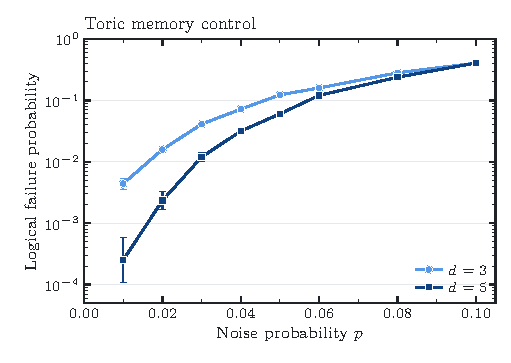
\includegraphics[width=\columnwidth]{phenomenological_mw_demo.pdf}
\caption{Code-capacity MWPM sanity check on toric codes at distances $3$ and $5$.  The plot shows the logical error rate under the finite code-capacity decoder test described in the surrounding text.}
\label{fig:supp-mw-demo}
\end{figure}

\paragraph{Gauging-rectangle sanity check (MWPM).}
Script \texttt{gauging\_rectangle\_mwpm.py} attaches a lattice-surgery-style path-strip gauging graph to a rotated surface-code logical $Z$ at $d\in\{3,5,7\}$, decodes the deformed CSS code with PyMatching under code-capacity $X/Z$ data noise, and writes \texttt{gauging\_rectangle\_mwpm.csv}.  Observed distance-like suppression: $d{=}5$ below $d{=}3$ for $p\le0.06$.  This is a deformed surface-code/path-strip building-block sanity check under code-capacity $X/Z$ data noise.
\begin{figure}[t]
\centering
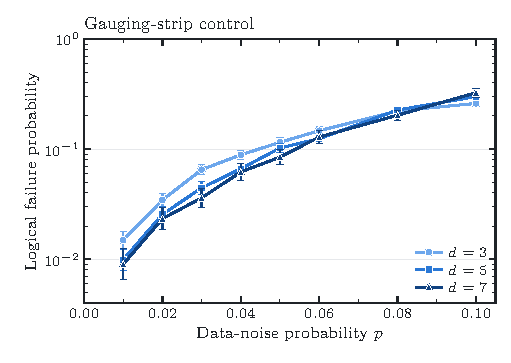
\includegraphics[width=\columnwidth]{gauging_rectangle_mwpm.pdf}
\caption{MWPM sanity check for the gauging-rectangle building block at $d\in\{3,5,7\}$.  The curves illustrate the expected distance-like suppression for the finite deformed surface-code/path-strip test instance.}
\label{fig:supp-gauging-mwpm}
\end{figure}

\paragraph{Analytic illustrations moved from the preceding analysis.}
The following plots visualize two closed-form bounds used in the proofs; they contain no fitted or simulated data and are kept here so the companion manuscript can prioritize the slab and architecture schematics.
\begin{figure}[t]
\centering
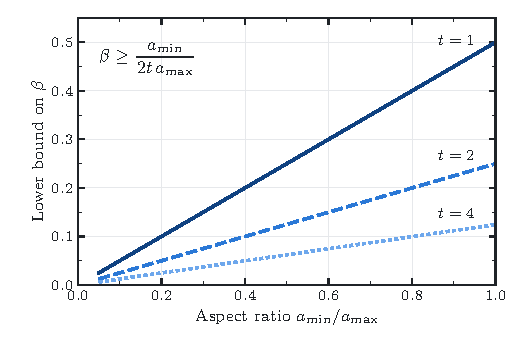
\includegraphics[width=\columnwidth]{relative_expansion_bound.pdf}
\caption{Analytic relative-expansion bound used in the local gauging argument.}
\label{fig:supp-relative-expansion}
\end{figure}

\begin{figure}[t]
\centering
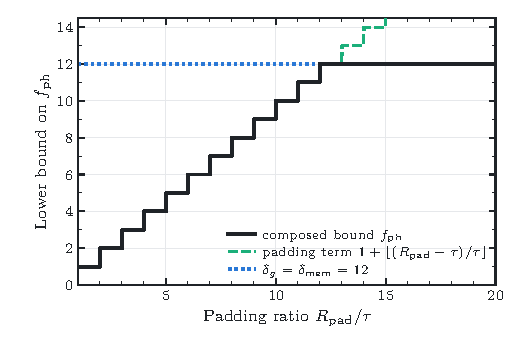
\includegraphics[width=\columnwidth]{padded_composition_bound.pdf}
\caption{Representative behavior of the padding term in the composed-distance bound.}
\label{fig:supp-padded-composition}
\end{figure}

\paragraph{Verification workflow.}
The complete finite verification sequence is recorded in \nolinkurl{run_verification.sh}; the cell-specific sequence is in \nolinkurl{run_bridge_verification.sh}. The revised package also records the deterministic checks rerun during preparation of these documents.




\section{Extended numerical results}
\label{sec:supp-numerics}
The numerical campaign combines algebraic checks with Monte Carlo tests of memory decoding, a local gauging primitive, a stage-composed schedule, and a continuous algebraic base$\rightarrow$gauged$\rightarrow$base code switch with persistent encoded data.  The scripts cover the source transcription, local incidence, detector identities, refinement moves, resource maps, and fault propagation.  These calculations characterize the implemented finite-size models; they do not assign a numerical value to the asymptotic threshold in the detailed universal resource theorem.

The circuit-level campaigns that show a clean crossing all use surface codes.  The gauging primitive uses the rotated surface code of distance $d$.  The stage-composed and continuous campaigns use the unrotated planar surface code of distance $L$, built as the hypergraph product of two length-$L$ repetition codes, with $n=L^2+(L-1)^2$ data qubits, and gauge a weight-$L$ logical representative with a strip of $L$ ancilla qubits.  They therefore test the gauging interface and the detector bookkeeping of a code switch, not the layer-code geometry.  The complete two-block measurement of Sec.~\ref{sec:two-block} runs on explicit layer-code blocks; the earlier truncated layer-code family, built from the single-chart cells, is retained only as the negative control of Sec.~\ref{sec:supp-negative}.

\subsection{Campaign setup}
The continuous code-switch circuit removes the main weakness of the earlier stage-composed model: the data block is never reset between the undeformed and deformed stages.  Its transition rules are algebraic rather than a gate-by-gate rendering of every Williamson--Baspin defect cell, so the three-dimensional realization still enters through the slab proof and junction-incidence construction.

The SI1000-like baseline assigns two-qubit depolarizing strength $p$, single-qubit and ordinary idle strength $p/10$, measurement flips $5p$, reset noise $2p$, and data idle-wait noise $2p$.  Stim detector error models are decoded by PyMatching MWPM.  The heavy and continuous headline runs use exact graphlike DEMs.

\begin{table*}[t]
\caption{Summary of the checks and numerical campaigns.}
\label{tab:supp-final-campaign}
\begin{tabular}{p{0.26\textwidth}p{0.48\textwidth}p{0.18\textwidth}}
\toprule
Item & Test & Result\\ \midrule
Explicit layer-code realization & complete check matrices, seven inputs; gluing forms, exhaustive words, walls & $k=K$; slab operators at every height (Table~\ref{tab:slab-certificate})\\
Archived cell certificate & all boundary words, full syndromes & non-discriminating; archived (Sec.~\ref{sec:archive})\\
Two-block layer-code measurement & complete circuits, Choi-state input, exact fault distance & Table~\ref{tab:two-block}\\
T8 extraction & single-location Pauli propagation & 10,008 faults; max image wt. 10\\
Resource maps & Steane and punctured RM15 algebraic maps & passed\\
Single-chart memory control (superseded) & BP--OSD, $L=3,4,5,6$ & crossing near $0.10$\\
Gauging primitive (rotated surface code) & exact-DEM SI1000-like MWPM, $d=3,5,7,9,11$ & crossing $\simeq4.12\times10^{-3}$\\
Stage-composed (planar surface code) & exact-DEM, $L=3,5,7,9,11$ & $4.64\times10^{-3}$ ($R=d$), $4.43\times10^{-3}$ ($R=2d$)\\
Continuous code switch (planar surface code) & base$\to$gauged$\to$base, $L=3,5,7,9,11$; $4.534\times10^6$ shots & Jeffreys crossing medians $4.47,4.43,4.33\times10^{-3}$ for $G=d,2d,3d$\\
Thin vs.\ thick interface & deformed-code construction on two 3D toric codes, $L=3$--$6$ & cut obstruction confirmed (Table~\ref{tab:interface-check})\\
Truncated single-chart SI1000-like (superseded) & incidence-based control & no clean four-size crossing\\
\bottomrule
\end{tabular}
\end{table*}

\subsection{Deterministic checks}
The source-cell script derives $H_{\rm end}$ and $H_{\rm mid}$ from the published condensation generators, including the $110$ middle-cell pass-through and the $X\leftrightarrow Z$ duals.  The slab theorem itself is checked on complete explicit codes (Sec.~\ref{sec:certificate}).

The prefix-parity recurrence is checked on all even words through length eight and on longer deterministic stress words.  The rank criterion is evaluated on concrete CSS instances; the stacked-toric control has minimum passing slab thickness $t=3$.  The two surface-code subdivision identities used for constant refinement are checked at the stabilizer level.

For the detector schedule, the scripts check T0--T7 parity matrices, boundary-state coordinates, transition relations, and fiber-product gluing.  The T8 routing calculation covers both CSS orientations, check weights $1$--$8$, and reversible shuttle words.  It enumerates 10,008 single-location nonidentity Pauli faults and finds maximum phenomenological image weight ten on this regression family.  The bounded-radius construction in the preceding analysis supplies the general route.

The resource calculations separately check one-bit teleportation, Pauli transport, $SS_XS=e^{i\pi/4}H$ up to phase, and the Steane $7\to1$ and punctured Reed--Muller $15\to1$ phase orientations.  The corrected factory circuit has zero logical failure in the noiseless checks.  A legacy factory diagnostic that failed at $p=0$ was traced to an encoding/convention mismatch and is not used.

The core scripts are \texttt{reproducibility\_checks.py}, \texttt{slab\_interface\_audit.py}, \texttt{glue\_example\_check.py}, and \texttt{factory\_map\_audit.py}.  CSV ledgers retain the slab cells, junction supports, refinement moves, T8 words and fault images, factory maps, and operational constants.

\subsection{Memory, gauging, and stage-composed controls}
\begin{figure*}[t]
\centering
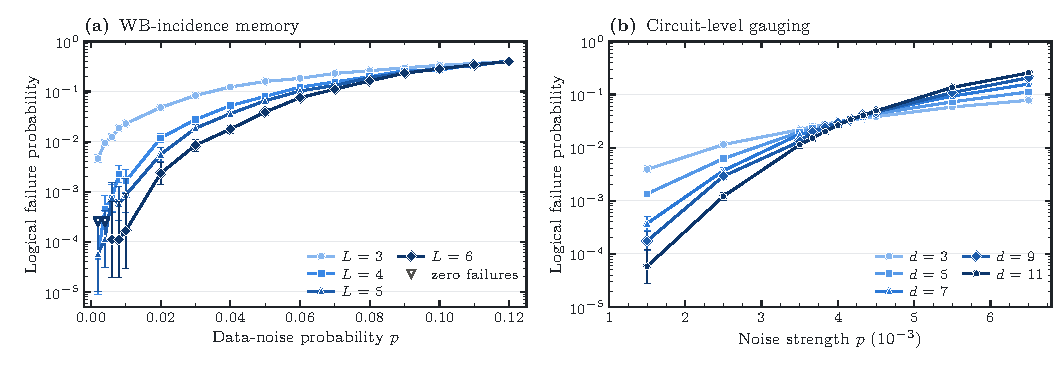
\includegraphics[width=\textwidth]{fig10_building_blocks.pdf}
\caption{Finite building-block diagnostics. (a) Code-capacity BP--OSD on the
truncated single-chart incidence family (superseded). (b) The exact-DEM circuit-level
gauging primitive under SI1000-like noise. Error bars are pointwise Wilson
95\% intervals. Open downward triangles denote the upper end of the Wilson
interval for a zero-failure observation. These are finite-model controls.}
\label{fig:building-controls}
\end{figure*}
\paragraph{Memory.}
The truncated single-chart incidence family (superseded; Sec.~\ref{sec:finite-cell-cert}) $L=3,4,5,6$ was decoded under independent code-capacity $X/Z$ noise with BP--OSD and the corrected CSS logical pairing.  Increasing-size suppression is separated at several low-$p$ points and the curves cross near $p\simeq0.10$.  A separate growing HGP memory family gives the same qualitative control behavior.

\paragraph{Gauging primitive.}
The local SI1000-like gauging primitive, on the rotated surface code, was extended to $d=3,5,7,9,11$.  All five sizes show monotone suppression at $p=1.5,2.5,3.5\times10^{-3}$; the smallest-versus-largest crossing is $p_\times\simeq4.12\times10^{-3}$.

\paragraph{Stage-composed schedule.}
Before the continuous transition circuit was built, a stage-composed protocol decoded the idle, noisy gauging, and final stages separately.  The campaign used five sizes through $L=11$, exact graphlike DEMs, and $3.955\times10^6$ Monte Carlo shots over 180 parameter points.  For $R=d$ the five-size ordering is Wilson-separated at $p=0.0015,0.0025,0.0035$, with crossing $4.64\times10^{-3}$.  For $R=2d$ the ordering remains separated through $p=0.004$, with crossing $4.43\times10^{-3}$.  In both schedules the fitted slope of $\log p_L$ changes sign across the crossing.

\begin{figure*}[t]
\centering
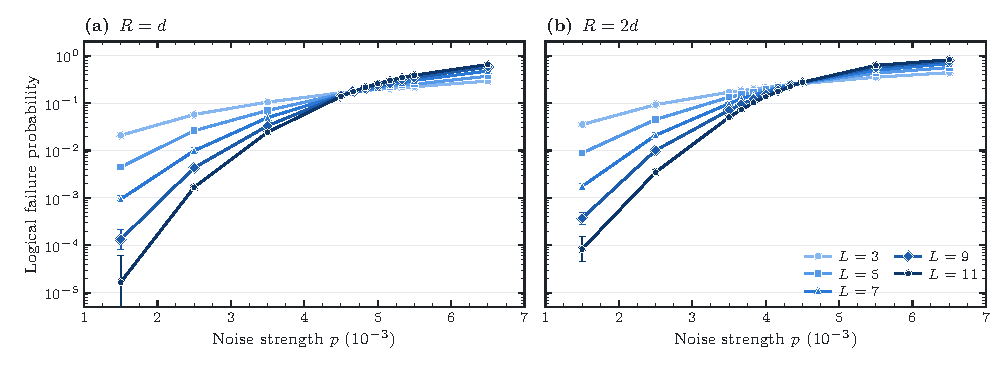
\includegraphics[width=0.94\textwidth]{supp_heavy_stage_composed.pdf}
\caption{Stage-composed SI1000-like stress test on planar surface codes (hypergraph products of repetition codes).  Five sizes $L=3,5,7,9,11$ retain low-$p$ suppression for both $R=d$ and $R=2d$; the smallest-versus-largest crossings are approximately $4.64\times10^{-3}$ and $4.43\times10^{-3}$.}
\label{fig:supp-heavy-stage}
\end{figure*}

\subsection{Continuous algebraic base$\rightarrow$gauged$\rightarrow$base code-switch circuits}
The largest numerical experiment keeps the same encoded data block, a planar surface code of distance $L$, through the entire algebraic code switch.  At entry, each old $X$ stabilizer is represented by a modified gauged generator together with strip operators whose product reproduces the undeformed check.  The deformed $ZZ$ joints are introduced simultaneously, and the code verifies $H_X^{\rm gauge}(H_Z^{\rm gauge})^T=0$ rather than deleting residual anticommuting rows.  The exit implements the inverse boundary relation.  Detector records span both transition edges and the repeated deformed rounds in one Stim circuit.

For each $L=3,5,7,9,11$, the final archived campaign tests $G=d,2d,3d$ (Fig.~\ref{fig:supp-continuous} and Table~\ref{tab:supp-continuous-crossing}).  The dataset contains 255 parameter points and $4.534\times10^6$ shots.  All 15 $p=0$ controls have zero failures, every transition-identity check passes, and every headline DEM is graphlike.  At $p=0.0035$ the end-to-end failure probabilities are
\begin{equation*}
\begin{array}{c|ccccc}
G & L=3&5&7&9&11\\\hline
 d &.1111&.0795&.0609&.0438&.0324\\
2d &.1308&.0924&.0729&.0511&.0399\\
3d &.1326&.1125&.0811&.0576&.0428
\end{array}
\end{equation*}
and the consecutive-size Wilson intervals are separated for these rows.  Five-size suppression remains monotone through at least $p=0.004$ for all three durations.  Consecutive-size Wilson intervals are separated at every tested $p$ from $0.0025$ to $0.00375$ for all three durations, and also at $p=0.0015$ for $G=d$ and $3d$; for $G=2d$ at $p=0.0015$ the $L=9$ and $L=11$ intervals overlap.

\begin{figure*}[t]
\centering
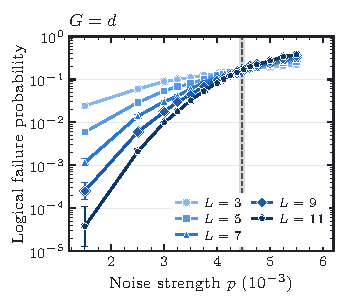
\includegraphics[width=0.325\textwidth]{threshold_G1d.pdf}\hfill
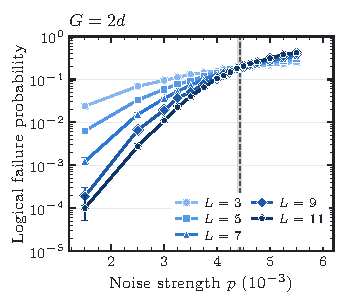
\includegraphics[width=0.325\textwidth]{threshold_G2d.pdf}\hfill
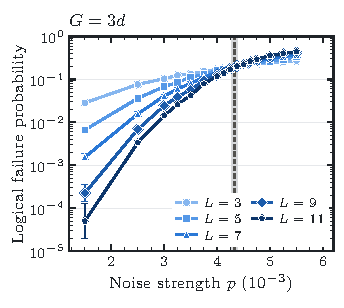
\includegraphics[width=0.325\textwidth]{threshold_G3d.pdf}
\caption{Continuous algebraic base$\rightarrow$gauged$\rightarrow$base code-switch circuit on the planar surface code of distance $L$ under the SI1000-like parameterization for $G=d,2d,3d$ (left to right).  The same encoded block is used throughout.  Pointwise bars are Wilson $95\%$ intervals; the vertical markers and gray bands show the smallest-versus-largest Jeffreys posterior crossing medians and conditional 95\% intervals.  The transition rules implement the stabilizer/check relations used by the model rather than a gate-by-gate rendering of every Williamson--Baspin defect cell.}
\label{fig:supp-continuous}
\end{figure*}

Sampling independent Jeffreys posteriors for the $L=3$ and $L=11$ binomial rates and linearly interpolating the first crossing gives medians $4.471\times10^{-3}$, $4.431\times10^{-3}$, and $4.328\times10^{-3}$ for $G=d,2d,3d$.  The corresponding conditional $95\%$ posterior crossing bands are $[4.426,4.522]$, $[4.392,4.466]$, and $[4.265,4.393]\times10^{-3}$.  Their full envelope is therefore $[4.265,4.522]\times10^{-3}$, but this envelope describes Monte Carlo/interpolation uncertainty only; it does not include finite-size-scaling or microscopic-model systematics.  Tripling the noisy gauged interval shifts the median crossing by about $3.2\%$.

\subsection{Finite-size scaling diagnostics}
A two-size crossing can be accidental, so the final campaign also records all-size monotonicity, Wilson-separated consecutive-size intervals, and the slope of $\log p_L$ versus $\log L$.  For each duration the slope is strongly negative at low $p$ and changes sign in the same $4.3$--$4.5\times10^{-3}$ region as the endpoint crossing.  This all-size trend is independent of the posterior calculation, which uses only the smallest and largest sizes.

\begin{table*}[t]
\caption{Continuous-circuit finite-size diagnostics.  The posterior bands are conditional on the smallest-versus-largest interpolation and are not systematic uncertainty bands for an asymptotic threshold.}
\label{tab:supp-continuous-crossing}
\scriptsize
\setlength{\tabcolsep}{4pt}
\begin{tabular}{c c c c c}
\toprule
$G$ & monotone through & Wilson-separated at & Jeffreys crossing median & conditional $95\%$ band\\\midrule
$d$  & $0.00425$  & $0.0015$--$0.00375$ & $4.471\times10^{-3}$ & $[4.426,4.522]\times10^{-3}$\\
$2d$ & $0.004125$ & $0.0025$--$0.00375$ & $4.431\times10^{-3}$ & $[4.392,4.466]\times10^{-3}$\\
$3d$ & $0.004125$ & $0.0015$--$0.00375$ & $4.328\times10^{-3}$ & $[4.265,4.393]\times10^{-3}$\\
\bottomrule
\end{tabular}
\end{table*}

At $p=0.0015$ the $G=d$ circuit decreases from $p_L=2.425\times10^{-2}$ at $L=3$ to $3.75\times10^{-5}$ at $L=11$, a factor of about $6.5\times10^2$.  This checks that the suppression seen at $L=3,5,7$ continues when $L=9,11$ are added.

Point-level CSV output includes shots, failures, Wilson bounds, exact-DEM and transition-check flags, detector/error counts, code sizes, round counts, and stopping conditions.  The archived final dataset and deterministic crossing analysis are in \nolinkurl{numerical/continuous_transition/threshold_estimate/}.

\subsection{Negative controls, factories, and interpretation}\label{sec:supp-negative}
The truncated single-chart incidence family (superseded; Sec.~\ref{sec:finite-cell-cert}) does not show a clean $L=3>4>5>6$ SI1000-like circuit-level crossing under the tested schedule.  Earlier WB circuit runs also required approximate DEM decomposition.  For that reason the headline circuit results use planar surface codes, whose detector error models are exactly graphlike; they do not test the layer-code geometry.

The source package retains the Steane and punctured Reed--Muller factory maps, finite SI1000-like probes with correct noiseless behavior, and three-dimensional routing coordinates.  These check the displayed gadget maps; they are not a multilevel factory-threshold calculation.  Coherent-overrotation and leakage toy models are also exploratory.  The local-stochastic Pauli theorem is not extended to general CPTP or leakage noise, and no efficient-decoder threshold is inferred from MWPM or BP--OSD performance.

\begin{figure*}[t]
\centering
\begin{minipage}{0.48\textwidth}\centering
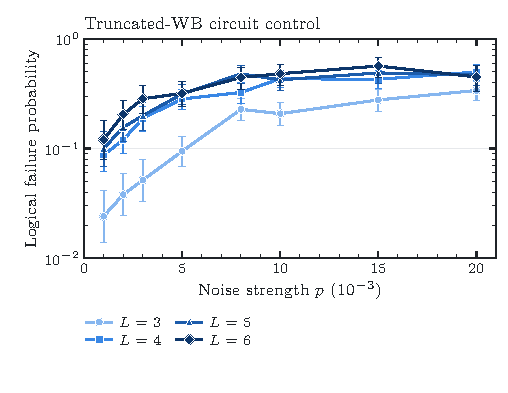
\includegraphics[width=\linewidth]{final_circuit_level_arch_si1000_wb.pdf}
\end{minipage}\hfill
\begin{minipage}{0.48\textwidth}\centering
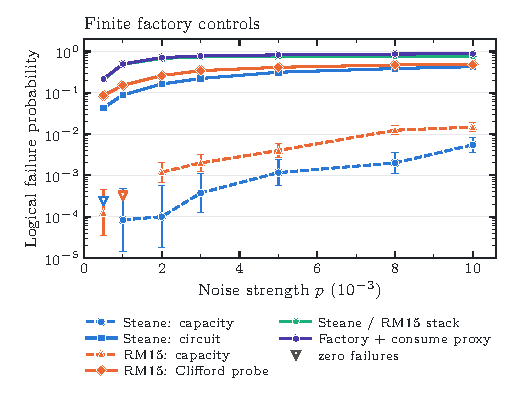
\includegraphics[width=\linewidth]{final_magic_factory_rm15_si1000.pdf}
\end{minipage}
\caption{Diagnostic controls.  Left: the truncated single-chart (superseded) SI1000-like schedule, which lacks the clean all-size ordering used for the headline result.  Right: finite Steane and Reed--Muller capacity, Clifford-circuit, and consumption-proxy controls with the proper noiseless convention. Open downward triangles denote the upper end of a Wilson 95\% interval at zero observed failures.}
\label{fig:supp-controls}
\end{figure*}

\subsection{Files and interpretation boundary}
The principal files are \nolinkurl{numerical/continuous_transition/final_transition_heavy.py}, the archived final crossing campaign in \nolinkurl{numerical/continuous_transition/threshold_estimate/} (including \nolinkurl{all_points.csv} and \nolinkurl{fit_threshold_estimate.py}), \nolinkurl{numerical/stage_composed/paper_stim_validation.py}, \nolinkurl{numerical/stage_composed/all_points.csv}, and \nolinkurl{numerical/stage_composed/HEAVY_VERIFICATION_REPORT.md}, together with the core verification scripts listed in \nolinkurl{run_verification.sh}.  The final continuous crossing campaign contains $4.534\times10^6$ shots and the stage-composed campaign $3.955\times10^6$ shots.

The arbitrary-size slab theorem for the explicit realization, Williamson--Yoder spacetime cleaning, the global restriction/composition proof, the existence of a positive committed-MW threshold, and the asymptotic resource bounds are analytic results.  The continuous model is an algebraic surface-code code-switch schedule with noisy detector histories and persistent encoded data; it does not reconstruct each published Williamson--Baspin defect cell as a gate-by-gate Stim circuit.  Accordingly, the observed $4.3$--$4.5\times10^{-3}$ structure is only a finite-size diagnostic of that model.

\section{Complete two-block measurement on explicit layer-code blocks}
\label{sec:two-block}

The surface-code campaigns of Sec.~\ref{sec:supp-numerics} prepare $Z$-basis
data and check one final logical-$Z$ observable, so they do not test the
reported measurement bit, both logical sectors, spectator logicals, or the
action on an unknown, entangled input.  The script
\texttt{two\_block\_measurement.py} tests all four on a complete circuit for
one joint logical measurement between two explicit layer-code blocks.

\paragraph{Circuit.}
Each block is the explicit realization of the $[[4,2,2]]$ input at spacing
$s=2$ ($n=224$, $K=2$, $d_X=5$, $d_Z=4$; Table~\ref{tab:explicit-distance}).
Logical qubit~1 of each block is measured jointly, $P=\overline X_1^{(a)}
\overline X_1^{(b)}$, by Williamson--Yoder gauging: an ancilla qubit on every
edge of a planar grid $G$ attached to the single-layer slab representatives
of Theorem~\ref{thm:slab-resolved} ($12$ port qubits per block), Gauss-law
checks on the grid vertices, unit-square flux checks, and the original $Z$
checks deformed along shortest grid paths.  Logical qubit~2 of each block is
a spectator.  Every check is measured with its own ancilla and CNOTs, $X$
checks before $Z$ checks in each round, for $2s=4$ rounds before, during, and
after the deformation.  The edges are prepared in $|0\rangle$ and read in $Z$,
and the gauging byproduct fixed by the edge readouts is applied to the Pauli
frame.  The noise is uniform circuit noise of strength $p$:
two-qubit depolarizing after every CNOT, one-qubit depolarizing on every data
and edge qubit in every round, and flips after every reset and before every
measurement, including the final data readout.

\paragraph{Input and observables.}
Each of the four logical qubits starts maximally entangled with a noiseless
reference qubit; the entangled input is prepared by noiseless multi-qubit
measurements whose outcomes enter the observables.  After the protocol, the
output Choi state is fixed by eight stabilizer generators, which are tested in
two experiments.  An $X$-basis readout tests the reported bit,
$m+x_{R_1^a}+x_{R_1^b}$, and the four $X$-sector frames
$\overline X_j^{(\cdot)}+x_{R_j^{(\cdot)}}$; a $Z$-basis readout tests
$\overline Z_1^{(a)}\overline Z_1^{(b)}+z_{R_1^a}+z_{R_1^b}$ and the two
spectator $Z$ frames.  Without noise all detectors and all eight observables are
deterministic and the protocol has zero failures, which certifies that the
circuit implements the projective measurement of $P$ with the correct
reported outcome and acts as the identity on both spectators, for an
arbitrary entangled input.

\paragraph{Interfaces.}
We compare grids that join the two port regions through a bridge of $w=1,2,3$
parallel rows (the ports of each block have their own planar grid), a single
planar grid spanning both blocks, and the same grid with two ancillas on every
edge.  The cut between the two blocks' ports has $1,2,3,5$ and $10$ edges,
respectively.

\paragraph{Short undetectable fault patterns.}
For every observable we compute the fault distance of the complete circuit,
the minimum number of fault mechanisms that flip it without firing a
detector, with the CP-SAT formulation of \texttt{min\_weight\_logical.py} (exactly where the solver proves optimality, otherwise as a bracket)
and the CSS sector reduction described there (Table~\ref{tab:two-block}).  The
deformed-code distances are computed the same way at the code level.  Cut
obstruction: the deformed code's $X$ distance equals the bridge width, and in
the circuit a single fault on the one-edge bridge flips
$\overline Z_1^{(a)}\overline Z_1^{(b)}$ undetectably.  This is the
Proposition~\ref{prop:cut-obstruction} logical $X(\delta T)$, realized as an
$X$ fault on the bridge edge that changes the byproduct frame by
$\overline X_1^{(a)}$.

\paragraph{Results.}
The reported bit $m$ has fault distance $4$ for every interface.  This equals
the number of deformed rounds, which bounds a timelike string of flipped
Gauss-law records.  The block distance $d_Z=4$ does not limit it: the
weight-$4$ $Z$ logicals flip only the spectator, and the lightest $Z$-type
operator of one block that anticommutes with $\overline X_1$ has weight $10$
(exact; \texttt{reported\_bit\_spacelike\_check.py}).  With $R=5$ rounds the
fault distance of $m$ is exactly $5$ through the three bridges and the
spanning grid (Sec.~\ref{sec:two-block-scaling}).  The spectators are unaffected by
the interface: their $X$ frames have fault distance $4=d_Z$ for every
interface, and their $Z$ frames are at least $4$ (at least $5$ for four of the
five interfaces).  The measured pair's $Z$ sector is where the interface
matters.  With a bridge of $w$ rows, the fault distance of
$\overline Z_1^{(a)}\overline Z_1^{(b)}$ is exactly $w$ for $w=1,2,3$: a single
fault on a one-edge bridge flips it undetectably, although both blocks have
distance at least four.  The planar grid spanning both blocks restores it to
exactly $5$, the blocks' $X$ distance; with two ancillas per edge the solver
proves at least $4$ and finds a pattern of weight $5$.  The deformed-code
distance $\widetilde d_X$ shows the same pattern at the code level ($w$ for the
bridges, $5$ for both grids).  The sampled failure rates of
$\overline Z_1^{(a)}\overline Z_1^{(b)}$ follow the same ordering: $71$, $68$
and $5$ failures in $1000$ shots for $w=1,2,3$ (Wilson $95\%$ intervals
$[5.7,8.9]\%$, $[5.4,8.5]\%$ and $[0.2,1.2]\%$), none for the grid (upper end
$0.38\%$), and $2$ for the doubled grid ($[0.05,0.73]\%$).  The one- and
two-row bridges fail at similar rates because an even width detects a single
bridge fault but cannot correct it (Sec.~\ref{sec:two-block-scaling}).  The failure rate of the reported
bit, $1.8$--$6.1\%$, does not improve with the interface, consistent with its
interface-independent fault distance; it is highest for the doubled grid,
whose Gauss-law checks have twice the weight.  The spectator frames fail in at
most $3$ of $1000$ shots in the $X$ sector and never in the $Z$ sector.  Every
run uses a recorded integer seed, listed in \nolinkurl{two_block_mc.csv}.
These blocks are small ($d\le5$), and the extraction measures each check with
its own ancilla rather than through the routed schedule of
Proposition~\ref{prop:nn-extraction}; the experiment tests the complete
logical action and the interface mechanism.  Section~\ref{sec:two-block-scaling}
repeats it at four block sizes, and Sec.~\ref{sec:two-block-routed} with the
routed schedule on three input codes.

\begin{table*}[t]
\caption{Complete two-block measurement on explicit $[[4,2,2]]$ layer-code
blocks ($s=2$, four rounds per phase).  ``Cut'' is the number of grid edges
separating the two blocks' ports; $\widetilde d_X$, $\widetilde d_Z$ are the
distances of the deformed code (exact; $^\ast$exact because the solver found
$4$ and Proposition~\ref{prop:gauging-distance} gives
$\widetilde d_Z\ge d_Z=4$).  The fault distances are for the complete
circuit and each observable; an entry $a$--$b$ means the solver proved a lower
bound $a$ and found an undetectable fault pattern of weight $b$ within its
time limit.  Failure rates are BP+LSD decoded at $p=0.002$ with
$1000$ shots per basis (four runs of $250$ with recorded seeds); a rate of
$0.0\%$ has Wilson $95\%$ upper end $0.38\%$.  ``Spect.'' is the spectator
$\overline X_2^{(a)}$ and $\overline Z_2^{(a)}$ frames.}
\label{tab:two-block}
\centering
\scriptsize
\setlength{\tabcolsep}{3.5pt}
\begin{tabular}{@{}lrrrrrrrrrrrr@{}}
\toprule
 & & & & & \multicolumn{5}{c}{circuit fault distance} & \multicolumn{3}{c}{failure rate} \\
\cmidrule(lr){6-10}\cmidrule(l){11-13}
Interface & edges & cut & $\widetilde d_X$ & $\widetilde d_Z$ & $m$ & $\overline X_1^{(a)}$ & $\overline X_2^{(a)}$ & $\overline Z_1\overline Z_1$ & $\overline Z_2^{(a)}$ & $m$ & $\overline Z_1\overline Z_1$ & spect.\ $X$/$Z$ \\
\midrule
bridge, $w=1$ & 156 & 1 & 1 & 4$^{\ast}$ & 4 & 4--10 & 4 & 1 & 4--12 & 2.7\% & 7.1\% & 0.1\%/0.0\% \\
bridge, $w=2$ & 163 & 2 & 2 & 4$^{\ast}$ & 4 & 4--12 & 4 & 2 & 5--12 & 1.8\% & 6.8\% & 0.2\%/0.0\% \\
bridge, $w=3$ & 170 & 3 & 3 & 4$^{\ast}$ & 4 & 4--10 & 4 & 3 & 5--13 & 3.2\% & 0.5\% & 0.2\%/0.0\% \\
grid, multiplicity 1 & 184 & 5 & 5 & 4$^{\ast}$ & 4 & 4--10 & 4 & 5 & 5--12 & 3.1\% & 0.0\% & 0.3\%/0.0\% \\
grid, multiplicity 2 & 368 & 10 & 5 & 4$^{\ast}$ & 4 & 4--10 & 4 & 4--5 & 5--12 & 6.1\% & 0.2\% & 0.1\%/0.0\% \\
\bottomrule
\end{tabular}
\end{table*}


\subsection{Scaling with block size}
\label{sec:two-block-scaling}
A second campaign repeats the measurement at four block sizes.  The circuits
come from \texttt{two\_block\_measurement.py}, generalized to iceberg inputs
$[[k+2,k,2]]$ and free spacing; for the parameters of
Table~\ref{tab:two-block} the generator produces the same circuits,
character for character.  Each block is the explicit realization of the
$[[4,2,2]]$ input at spacing $s=2,3,4,5$ ($n=224$, $504$, $896$, $1400$;
$d_X=2s+1$ and $d_Z=2s$, Table~\ref{tab:explicit-distance}), or of the
$[[6,4,2]]$ input ($K=4$) at $s=2,3,4$.  Every phase has $R=2s+1$ rounds, at
least both block distances.  The interfaces are the one-row bridge at every
size, bridges of $w=2,3$ rows at $s=3,4$, the spanning grid with one or two
ancillas per edge, and, as a baseline, the same blocks idling for the same
$3R$ rounds without gauging.  The noise model, input and observables are
those above, at $p\in\{0.5,1,2,3,4,6\}\times10^{-3}$.

\paragraph{Decoding and sampling.}
At these sizes the full-model decoder of Table~\ref{tab:two-block} takes
seconds per shot, so each experiment is decoded on the detectors of its own
CSS sector (the $X$ checks and Gauss laws for the $X$ experiment, the $Z$ and
flux checks for the $Z$ experiment) with the same BP and LSD settings;
mechanisms with the same restricted syndrome and observable effect are
merged.  Every fault is still sampled; the decoder only ignores the
correlation that a $Y$ fault induces between the sectors.  A paired check on
identical shots at $s=2$ (\texttt{decoder\_check.py}, $2000$ shots per point)
compares it with the full-model decoder.  Through the spanning grid at
$p=3\times10^{-3}$ the full-model decoder fails in $79$ shots of the $X$
experiment against $162$ for the per-sector decoder (exact McNemar test on the
discordant shots, $p$-value $7\times10^{-10}$) and in $20$ against $31$ shots of the $Z$
experiment ($p$-value $0.11$); through the one-row bridge at $p=2\times10^{-3}$ it fails
in $212$ against $224$ shots ($p$-value $0.07$).  The per-sector decoder is therefore
pessimistic for the spanning grid, by up to a factor of two at this point, and
nearly matches the full-model decoder for the bridge, whose failures are
undetectable faults; the contrast between the interfaces reported below is,
if anything, understated.  The per-sector decoder is $34$ to $62$ times faster.  Shots are drawn in
batches of fixed size with recorded seeds.  Each point ran until $200$ failed
shots, a shot cap, or the end of a $36$-hour budget on eight cores, with
unfinished points sharing the remaining time: $3.0\times10^6$ shots and
$237$ core-hours in total.  At $s\ge4$ and $p\ge3\times10^{-3}$ the decoder
exceeded the $16$\,GB memory in several runs, so ten of the $206$ points have
no data and several have few shots; these points lie near or above the
crossing and are not used below.  The runner, the circuits and every batch
with its seed are in \nolinkurl{scaling_campaign/} and
\nolinkurl{numerical/scaling_campaign/}; \texttt{make\_scaling\_figure.py}
generates Table~\ref{tab:two-block-scaling}, Fig.~\ref{fig:two-block-scaling}
and every number quoted here from the batch file, the paired-check file and
the distance files.

\paragraph{Thin bridge versus spanning grid.}
Through the one-row bridge the failure rate of
$\overline Z_1^{(a)}\overline Z_1^{(b)}$ rises with the block size: from
$3.9\%$ at $s=2$ to $8.8\%$ at $s=5$ at $p=10^{-3}$, and from $2.3\%$ to
$4.8\%$ at $p=5\times10^{-4}$.  A fault on the bridge edge is never detected,
and the edge is exposed in every one of the $R$ deformed rounds, which grow
with the blocks.  Through the spanning grid the same observable falls, from
$8.2\times10^{-4}$ at $s=2$ to $1.1\times10^{-4}$ at $s=5$ (one failure in
$9300$ shots) at $p=10^{-3}$, and at every size it agrees within the Wilson
intervals with the idle blocks.  At $s=5$ the two interfaces differ by more
than two orders of magnitude (Table~\ref{tab:two-block-scaling},
Fig.~\ref{fig:two-block-scaling}a,b).  This is
Proposition~\ref{prop:cut-obstruction} at growing size: the block distance
grows, the cut does not.

\paragraph{Fault distances at two sizes.}
The fault distances of $\overline Z_1^{(a)}\overline Z_1^{(b)}$ and of the
reported bit in Table~\ref{tab:two-block} were recomputed for the circuits of
this section ($R=2s+1$ rounds per phase) at $s=2$ and $s=3$, for the three
bridges and the spanning grid with one ancilla per edge, with the same CP-SAT
formulation and $30$ minutes per observable
(\texttt{run\_distances.py},
\nolinkurl{numerical/scaling_campaign/fault_distance.csv}).  Through a bridge
of $w=1,2,3$ rows the fault distance of
$\overline Z_1^{(a)}\overline Z_1^{(b)}$ is exactly $w$ at both sizes, although
the blocks' $X$ distance grows from $5$ to $7$.  Through the spanning grid it
is exactly $5=d_X$ at $s=2$; at $s=3$ the solver finds an undetectable
pattern of weight $7=d_X$ and proves a lower bound of $4$.  The reported bit
has fault distance exactly $5=R$ for all four interfaces at $s=2$, and between
$5$ and $7=R$ at $s=3$.  This is consistent with a limit set by the number of
rounds, as at $R=4$: the lightest spacelike $Z$ operator that flips it has
weight $10$ at $s=2$ and $15$ at $s=3$.

\paragraph{Suppression with size.}
For the spanning grid every observable improves with size below the
crossing.  A linear fit of $\ln(\text{failure})$ in $s$, weighted by the
failure counts, gives a suppression factor per unit of spacing
$\Lambda=4.8$ $[3.6,6.3]$ for the $X$ experiment (reported bit and all $X$
frames) and $\Lambda=2.6$ $[1.7,3.8]$ for the $Z$ experiment at $p=10^{-3}$,
decreasing to $1.11$ $[1.01,1.21]$ and $0.98$ $[0.86,1.12]$ at
$p=6\times10^{-3}$ (Fig.~\ref{fig:two-block-scaling}c; brackets are $95\%$
intervals).  With this decoder the finite-size crossing of the complete joint
measurement therefore lies near $p\approx6\times10^{-3}$.  The reported bit
alone fails in $101$ of $58000$ shots at $s=2$ and in $3$ of $22200$ at $s=4$
($p=10^{-3}$).

\paragraph{Bridge width.}
At $s=3$ and $4$ and $p=2\times10^{-3}$ the two-row bridge fails in $10.8\%$
and $16.0\%$ of shots, hardly better than the one-row bridge ($13.8\%$,
$17.0\%$), while the three-row bridge fails in $2.6\%$ and $2.4\%$.  This is
the pattern of an even distance: the two bridge edges that cross the cut bound
the same flux square, so an $X$ fault on either has the same syndrome, and the
two corrections differ by the cut logical $X(\delta T)$.  A single bridge fault
is detected but not corrected; three rows correct it.

\paragraph{More logical qubits and doubled edges.}
The $[[6,4,2]]$ blocks show the same ordering: at $p=10^{-3}$,
$\overline Z_1^{(a)}\overline Z_1^{(b)}$ fails in $4.9\%$, $5.2\%$ and $8.7\%$
of shots through the bridge and at rates $1.2\times10^{-3}$,
$1.8\times10^{-4}$ and $1.3\times10^{-4}$ through the grid at $s=2,3,4$, and
the six spectator $X$ frames have $240$, $42$ and $2$ failures in $26000$,
$20400$ and $17100$ shots.  At $p=10^{-3}$ two ancillas per edge leave the
rates of $\overline Z_1^{(a)}\overline Z_1^{(b)}$ within the intervals of one
ancilla per edge, but make the reported bit worse at the smallest size
($5.6\times10^{-3}$ against $1.7\times10^{-3}$ at $s=2$, $p=10^{-3}$), since each
Gauss law has twice the weight; the difference closes with size
($1.7\times10^{-4}$ against $1.4\times10^{-4}$ at $s=4$).

\paragraph{Scope.}
These are finite sizes of a family that grows the spacing of $d_{\rm in}=2$
inputs, with one ancilla per check rather than the routed schedule of
Proposition~\ref{prop:nn-extraction} (Sec.~\ref{sec:two-block-routed} uses
it), decoded by a particular heuristic decoder.  They show the cut obstruction and the protection of the spanning
grid at growing size, and a suppression factor above one for the complete
joint measurement below $p\approx6\times10^{-3}$; they do not estimate the
threshold of Theorem~\ref{thm:A24}, which concerns the committed
minimum-weight decoder.

\begin{table*}[t]
\caption{Failures of $\overline Z_1^{(a)}\overline Z_1^{(b)}$ (failed
shots/shots) in the scaling campaign: two $[[4,2,2]]$-input blocks at spacing
$s$, block distances $(d_X,d_Z)=(2s+1,2s)$, $R=2s+1$ rounds per phase,
uniform circuit noise $p$, per-sector BP+LSD.  ``Idle'' is the same blocks
for the same time without gauging.  An entry $0/n$ has Wilson $95\%$ upper end
about $3.8/n$; ``--'' was not run.}
\label{tab:two-block-scaling}
\centering
\small
\begin{tabular}{@{}llrrrr@{}}
\toprule
 & & \multicolumn{4}{c}{spacing $s$ \;$(d_X,d_Z)$} \\
\cmidrule(l){3-6}
$p$ & interface & $2$ \;$(5,4)$ & $3$ \;$(7,6)$ & $4$ \;$(9,8)$ & $5$ \;$(11,10)$ \\
\midrule
% generated by make_scaling_figure.py (two_block_scaling_table.tex)
$0.5\times10^{-3}$ & thin bridge, $w=1$ & 46/2000 & 279/9600 & 145/3600 & 72/1500 \\
 & spanning grid & 24/196000 & 1/72600 & 0/23400 & 0/9450 \\
 & idle & 27/264000 & 0/78000 & 0/23100 & 0/9000 \\
\addlinespace[2pt]
$1\times10^{-3}$ & thin bridge, $w=1$ & 78/2000 & 30/600 & 342/4500 & 252/2850 \\
 & spanning grid & 28/34000 & 13/69000 & 3/22800 & 1/9300 \\
 & idle & 31/44000 & 10/66600 & 0/23400 & 0/9150 \\
\addlinespace[2pt]
$2\times10^{-3}$ & thin bridge, $w=1$ & 176/2000 & 83/600 & 51/300 & 24/150 \\
 & spanning grid & 212/38000 & 26/14400 & 19/13500 & 1/1200 \\
 & idle & 64/20000 & 23/19200 & 18/19800 & 6/9000 \\
\addlinespace[2pt]
$3\times10^{-3}$ & thin bridge, $w=1$ & 315/2000 & 135/600 & 56/300 & 36/150 \\
 & spanning grid & 32/2000 & 49/4200 & 26/5100 & 0/150 \\
 & idle & 178/16000 & 34/5400 & 22/5700 & 22/4800 \\
\addlinespace[2pt]
$2\times10^{-3}$ & thin bridge, $w=2$ & -- & 65/600 & 48/300 & -- \\
$2\times10^{-3}$ & thin bridge, $w=3$ & -- & 46/1800 & 22/900 & -- \\
\bottomrule
\end{tabular}
\end{table*}

\begin{figure*}[t]
\centering
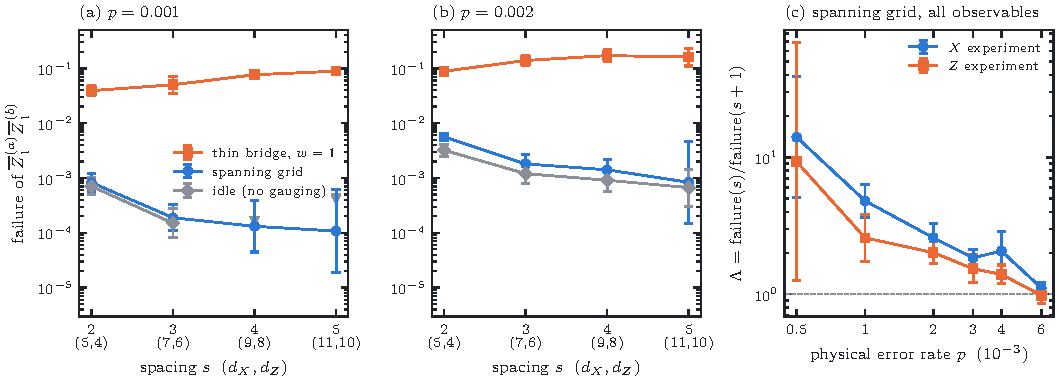
\includegraphics[width=\textwidth]{two_block_scaling.pdf}
\caption{Joint measurement at growing block size.  (a,b) Failure of the
measured pair's $Z$ sector through the one-row bridge, the spanning grid, and
for the same blocks idling without gauging, at $p=10^{-3}$ and
$2\times10^{-3}$; bars are Wilson $95\%$ intervals and open triangles the
upper end at zero failures.  The bridge gets worse as the blocks grow, the
grid gets better and tracks the idle blocks.  (c) Suppression factor per unit
of spacing for the spanning grid (all observables of each experiment),
weighted fit over the available sizes with $95\%$ intervals; it reaches one
near $p\approx6\times10^{-3}$.}
\label{fig:two-block-scaling}
\end{figure*}


\subsection{Routed nearest-neighbor extraction and growing inputs}
\label{sec:two-block-routed}
The circuits of Secs.~\ref{sec:two-block} and~\ref{sec:two-block-scaling}
measure every check with its own ancilla, and they grow only the spacing of
inputs with $d^{\rm in}=2$.  A third campaign replaces that extraction by the
routed schedule of Proposition~\ref{prop:nn-extraction} and grows the input
code at fixed spacing $s=2$.  It reports noiseless certification and exact
fault distances; it reports no failure rates, for the reasons given at the
end of this subsection.

\paragraph{Circuit.}
Every check has one routing ancilla, prepared and measured in the basis of
the check.  The ancilla moves by nearest-neighbor SWAPs along a depth-first
traversal of the lexicographically first spanning tree of a reserved routing
graph, applies the data--ancilla CNOT on its first visit to the contact site
of each support qubit, and retraces its path before readout.  Extraction
words whose sites overlap are separated by a greedy coloring and run in
sequential color classes.  The routing sites are an explicit
three-dimensional embedding of the layer-code edges, with an additional
sheet for the gauging edge qubits.  The noise is that of
Sec.~\ref{sec:two-block} with the routing included: two-qubit depolarizing
noise of strength $p$ after every CNOT and every SWAP, flips of probability
$p$ at every preparation and measurement, and one-qubit depolarizing noise
of strength $p$ on every data qubit, and on every routing qubit of the active
color class, in every time step in which it waits.  Each phase (before,
during and after the deformation) has $R$ rounds.  The interfaces are the
one-row bridge and the spanning grid with one ancilla per edge, and the
control is the same blocks idling for $3R$ rounds.

\paragraph{Inputs.}
The inputs are the $[[4,2,2]]$ code of Sec.~\ref{sec:two-block}; a six-qubit
band code with $H_X=H_Z$ formed by the checks $111100$ and $001111$, a
$[[6,2,2]]$ code with $\eta=2$; and the Steane code $[[7,1,3]]$.  At $s=2$
their realizations have $n=224$, $720$ and $1792$ qubits and
$L_x=L_z=4$, $6$ and $8$.  Their distances are $(d_X,d_Z)=(5,4)$
(Table~\ref{tab:explicit-distance}); $d_X\ge7$ and $d_Z=6$, where the bounds
are those of Theorem~\ref{thm:explicit-distance} and an operator of weight
six attains the second (below); and $d_X\ge18$, $d_Z\ge16$ by the same
theorem.  The routed circuits have $2352$ to $3144$, $7200$ to $9842$ and
$14118$ to $16293$ qubits from idle memory to the spanning grid, of which
$2507$, $7448$ and $12085$ are routing sites in the grid circuit.  The
coloring uses $7$, $10$ to $11$, and $11$ to $13$ classes for the $X$ and $Z$
checks of the blocks, and $8$ to $11$, $20$ to $31$, and $12$ to $19$ for the
Gauss-law and flux checks; the median ancilla tour has $24$, $26$ and $24$ shuttle steps (the longest $143$,
$189$ and $123$).  The bridge crosses between the two blocks in one edge for
every input, the grid in $5$, $17$ and $9$ edges.

\paragraph{Certification.}
Without noise every detector is silent and every observable takes its
correct value in all $40$ circuits run, $28$ measurements and $12$ idle
controls (three inputs, both bases, and the round numbers of
Table~\ref{tab:two-block-routed}): the reported bit, the $X$ and $Z$ frames of
the measured pair, and those of the spectators.  The routed circuit therefore
implements the projective measurement with the correct outcome and leaves the
spectators untouched, as the colocated circuit does.

\paragraph{Fault distances.}
The fault distances use the CP-SAT formulation and sector reduction of
Sec.~\ref{sec:two-block}, with a time limit per observable between a few
minutes and a few hours; for the band grid and idle circuits at $R=7$ the solver instead
decides whether an undetectable pattern of weight at most six exists, for up
to $8.7$ hours (Table~\ref{tab:two-block-routed}).  Four results hold.

(i) The cut obstruction survives routing and growing inputs.  Through the
one-row bridge the fault distance of $\overline Z_1^{(a)}\overline Z_1^{(b)}$
is exactly one for all three inputs and every $R$ tested, while the blocks'
$X$ distance grows from $5$ to at least $7$ and at least $18$.

(ii) On the $[[4,2,2]]$ blocks the routed grid keeps the full distance.  Its
fault distance for $\overline Z_1^{(a)}\overline Z_1^{(b)}$ is exactly $5$ at
$R=2$, $3$ and $5$, and the same blocks left idle also give exactly $5$, as do
the colocated circuits (Table~\ref{tab:two-block}).  The grid therefore
removes nothing from the distance that storage alone provides.  For the band
and Steane blocks the grid distance is not resolved: the lower bounds are $4$
to $5$, and the lightest patterns found have weight $17$ and $9$, the number
of grid edges crossing between the blocks.  For the Steane input that number
is $9$, so by Proposition~\ref{prop:cut-obstruction} the deformed code has
$X$ distance at most $9$, below the block's $d_X\ge18$.  This is the case in
which Corollary~\ref{cor:edge-multiplicity} needs more than one ancilla per
edge; a run with two (crossing number $18$, the lower bound on $d_X$) was
prepared but not carried out.

(iii) The reported bit is limited by the number of rounds or by the lightest
$Z$-type operator that anticommutes with the measured logical, whichever is
smaller.  On the $[[4,2,2]]$ blocks its fault distance is exactly $R$ for
$R=2$, $3$ and $5$ through both interfaces; the lightest such operator has
weight $10$ (Sec.~\ref{sec:two-block}).  On the band blocks it is exactly $R$
for $R=2$ and $4$.  At $R=7$ the solver finds undetectable patterns of weight
$6$ through both interfaces, which flip $\overline X_1^{(a)}$ together with
the bit, and a pattern of weight $6$ for the $\overline X_1^{(a)}$ frame of
the idle blocks.  A spacelike operator of the block accounts for this weight:
the lightest $Z$-type operator of the band block that anticommutes with
$\overline X_1$ has weight exactly $6$ (\texttt{band\_spacelike\_check.py}),
which is the block's $Z$ distance, so no extraction schedule can give the bit
more than $\min\{R,6\}$, and $R=7$, the lower bound on $d_X$, cannot give it
$7$.  This is consistent with the bound
$\delta_g^{\rm rel}\ge\min\{\beta_0d,R_g\}$ of Eq.~(A15d), in which $d$ is
the least distance of the blocks involved.  The solver proves only $4$
(bridge) and $2$ (grid, idle), so whether routing adds lighter patterns is
open.  The spacelike limit depends on the logical class: for the class of the
input word $110000$ the lightest anticommuting $Z$-type operator has weight
$16$ to $24$ (CP-SAT bracket), against $6$ for $\overline X_1$ and for the
third class.

(iv) The frames of the blocks do not depend on the interface.  On the
$[[4,2,2]]$ blocks at $R=5$ the spectator $X$ frames have fault distance
exactly $4=d_Z$ for the bridge, the grid and idle memory, and $4$ is also the
weight of the lightest $Z$-type operator anticommuting with $\overline X_2$
(Sec.~\ref{sec:two-block}).  For all three, the measured $X$ frames have
patterns of weight $10$, the spacelike value, with lower bounds $5$ to $6$,
and the spectator $Z$ frames have patterns of weight $12$ with lower bound
$6$.  On the band blocks the spectator frames are not resolved (lower bounds
$3$ to $5$).

\paragraph{Sampled failure rates and the decoder.}
At $R\le2$ and $p=5\times10^{-4}$ to $2\times10^{-3}$, with the per-sector
BP+LSD decoder of Sec.~\ref{sec:two-block-scaling}, the target observable
fails in between a quarter and two thirds of the shots for every input,
interface and noise strength, idle memory included (for example $41$ of $80$ shots for the idle $[[4,2,2]]$
blocks at $p=5\times10^{-4}$), so these runs do not compare interfaces.  Two
features of these runs limit what they can show.  The routed schedule is
long: the longest ancilla tour on
the $[[4,2,2]]$ blocks has $143$ shuttle steps, so a round lasts at least
that many time steps, in each of which almost every data qubit receives
depolarizing noise of strength $p$; at $p=5\times10^{-4}$ this alone gives
each data qubit an error probability of about $0.07$ per round.  The decoder,
moreover, is not minimum weight.  An exhaustive test of every single
mechanism on the $[[4,2,2]]$ blocks at $R=3$ finds that it leaves $56$ of $81{,}332$ uncorrected in the
$Z$ sector of idle memory, $102$ of $85{,}260$ in its $X$ sector, and $2943$
of $93{,}385$ for the reported bit through the bridge, although a
minimum-weight decoder corrects every single mechanism at these fault
distances and none of them is undetectable.  The detector error models are
not graphlike, so matching does not apply.  For the routed circuits we
therefore use exact fault distances only.

\paragraph{Scope.}
The inputs grow in length but stay far from the balanced regime
($n^{\rm in}\le7$, $K\le2$), the grid has one ancilla per edge, and the grid
distance is resolved only for the $[[4,2,2]]$ blocks; the band grid, the
band idle $Z$ frame and a long-schedule Steane run remain open.  The campaign
tests the routed construction of Proposition~\ref{prop:nn-extraction} at
finite size and does not estimate a threshold.  The directory
\nolinkurl{numerical/routed_campaign/} holds every table, the noiseless
certification, the solver logs and the lightest undetectable pattern found
for every observable with an upper bound; \texttt{routed\_campaign\_check.py}
checks the
certification rows and that every archived pattern is undetectable and flips
its observable.

\begin{table*}[t]
\caption{Fault distances of the routed two-block circuits
(Proposition~\ref{prop:nn-extraction}; spacing $s=2$, one ancilla per grid
edge, $R$ rounds per phase).  An entry $a$--$b$ means the solver proved a
lower bound $a$ and found an undetectable pattern of weight $b$; ${\ge}a$
means a lower bound without a pattern; ``--'' was not computed.  ``Cut'' is
the number of edges crossing between the blocks (bridge/grid).  The block
distances of the band and Steane inputs are the bounds of
Theorem~\ref{thm:explicit-distance}, except $d_Z=6$ for the band (attained,
see text).  The lightest $Z$-type operator anticommuting with
$\overline X_1$ has weight $10$ for $[[4,2,2]]$ and $6$ for the band block,
and with $\overline X_2$ weight $4$ for $[[4,2,2]]$.}
\label{tab:two-block-routed}
\centering
\scriptsize
\setlength{\tabcolsep}{3.2pt}
\begin{tabular}{@{}lccrrrrrrrrrrrr@{}}
\toprule
 & & & & \multicolumn{3}{c}{$\overline Z_1^{(a)}\overline Z_1^{(b)}$} & \multicolumn{2}{c}{reported bit $m$} & \multicolumn{3}{c}{$\overline X_1^{(a)}$} & \multicolumn{3}{c}{spectator $\overline X_2^{(a)}$} \\
\cmidrule(lr){5-7}\cmidrule(lr){8-9}\cmidrule(lr){10-12}\cmidrule(l){13-15}
Input & $(d_X,d_Z)$ & cut & $R$ & bridge & grid & idle & bridge & grid & bridge & grid & idle & bridge & grid & idle \\
\midrule
$[[4,2,2]]$ & $(5,4)$ & 1/5 & 2 & 1 & 5 & -- & 2 & 2 & -- & -- & -- & -- & -- & -- \\
 & & & 3 & 1 & 5 & 5 & 3 & 3 & -- & -- & 6--10 & -- & -- & -- \\
 & & & 5 & 1 & 5 & 5 & 5 & 5 & 5--10 & 5--10 & 6--10 & 4 & 4 & 4 \\
\addlinespace[2pt]
band $[[6,2,2]]$ & $({\ge}7,6)$ & 1/17 & 2 & 1 & 5--17 & -- & 2 & 2 & -- & -- & -- & -- & -- & -- \\
 & & & 4 & 1 & 5--17 & -- & 4 & 4 & -- & -- & -- & -- & -- & -- \\
 & & & 7 & 1 & ${\ge}4$ & ${\ge}4$ & 4--6 & 2--6 & 4--6 & 4--6 & 2--6 & 5--24 & ${\ge}3$ & -- \\
\addlinespace[2pt]
Steane $[[7,1,3]]$ & $({\ge}18,{\ge}16)$ & 1/9 & 1 & 1 & 4--9 & -- & 1 & 1 & -- & -- & -- & -- & -- & -- \\
\bottomrule
\end{tabular}
\end{table*}


\section{Hardware demonstrations}
\label{sec:hardware}

\paragraph{The idea in plain terms.}
The distance results of Sec.~\ref{sec:gauging} rest on three mechanisms that
already appear in very small circuits.  A joint logical measurement through a
narrow interface can be undone by a few faults on that interface
(Proposition~\ref{prop:cut-obstruction}); parallel ancillas on an interface
edge widen every wall that crosses it
(Corollary~\ref{cor:edge-multiplicity}); and a wrong outcome in one round of
the measurement is caught by the next round
(Proposition~\ref{prop:slice-bound}).  This section tests each mechanism on
superconducting processors with blocks of three qubits.  It does not test
layer codes, the grid expansion, or the architecture, which need far larger
devices.

\begin{figure*}[t]
\centering
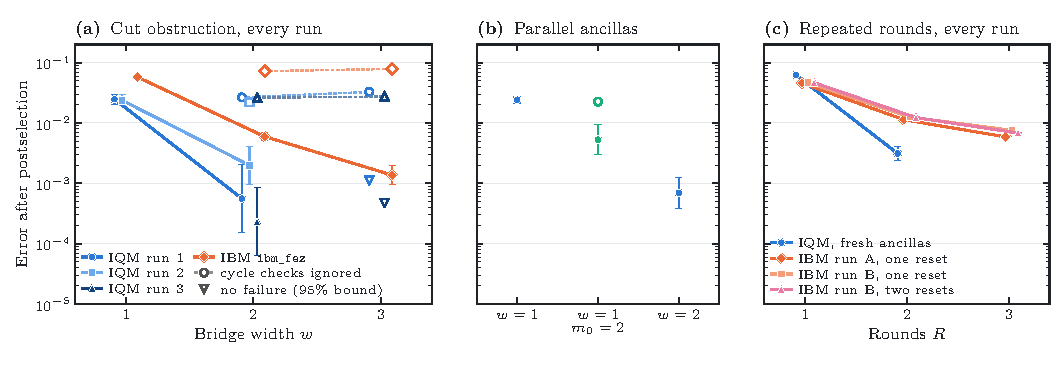
\includegraphics[width=\textwidth]{hardware_results.pdf}
\caption{Every hardware run separately (the main-text hardware figure pools
the IQM runs); error after postselection on every detector, with Wilson 95\%
intervals (open triangles: Wilson upper ends of zero counts).  (a)~Two
three-qubit blocks joined by a bridge of $w$ edges; open symbols: the same
samples with the bridge cycle checks ignored.  (b)~One bridge edge with two
parallel ancillas ($m_0=2$, aqua) against one bridge qubit and two bridge
edges, on IQM, each width pooled over every IQM run that has it; open symbol:
the bundle cycle ignored.  (c)~Reported-bit error against the number of
rounds; IQM uses fresh ancillas in every round, IBM measures and resets them,
once or twice.  Data in Tables~\ref{tab:hardware-cut}
and~\ref{tab:hardware-rounds}.}
\label{fig:hardware-sm}
\end{figure*}

\begin{table*}[t]
\caption{Cut obstruction and edge multiplicity on hardware.  Two three-qubit blocks joined by a bridge of $w$ edges ($w=0$: no gauging); $m_0=2$ puts two parallel ancillas on a single bridge edge.  Errors are postselected on every detector, in percent, with Wilson 95\% intervals; a zero count shows the upper end.  Control: the same shots postselected on the block checks only, ignoring the cycle checks that the extra bridge edges create.  Model: uniform circuit noise (IQM: CZ error $0.5\%$, readout $2\%/4\%$) or typical published medians (IBM), fixed before the run.  Generated by \texttt{hardware/hardware\_summary.py}.}
\label{tab:hardware-cut}
\begin{ruledtabular}
\begin{tabular}{llrrrlll}
Device, run & Bridge & Shots & Kept & Wrong & Error (\%) & Control (\%) & Model (\%)\\
\hline
IQM Emerald{,} run 1 & $w=1$ & 5{,}000 & 3{,}911 & 97 & 2.5 [2.0{,} 3.0] &  & 4.2\\
 & $w=2$ & 5{,}000 & 3{,}571 & 2 & 0.056 [0.015{,} 0.20] & 2.7 & 0.22\\
 & $w=3$ & 5{,}000 & 3{,}424 & 0 & $0$ ($\le0.11$) & 3.3 & 0.022\\
\hline
IQM Emerald{,} run 2 & $w=1$ & 5{,}000 & 3{,}820 & 91 & 2.4 [1.9{,} 2.9] &  & 4.2\\
 & $w=2$ & 5{,}000 & 3{,}513 & 7 & 0.20 [0.097{,} 0.41] & 2.2 & 0.19\\
\hline
IQM Emerald{,} run 3 & $w=2$ & 12{,}000 & 8{,}700 & 2 & 0.023 [0.0063{,} 0.084] & 2.6 & 0.22\\
 & $w=3$ & 12{,}000 & 8{,}105 & 0 & $0$ ($\le0.047$) & 2.8 & 0.022\\
\hline
IBM \texttt{ibm\_fez} & $w=0$ & 50{,}000 & 47{,}715 & 1 & 0.0021 [0.00037{,} 0.012] &  & 0.0023\\
 & $w=1$ & 50{,}000 & 27{,}931 & 1{,}611 & 5.8 [5.5{,} 6.0] &  & 3.3\\
 & $w=2$ & 50{,}000 & 24{,}220 & 144 & 0.59 [0.51{,} 0.70] & 7.2 & 0.16\\
 & $w=3$ & 50{,}000 & 21{,}181 & 29 & 0.14 [0.095{,} 0.20] & 7.9 & 0.012\\
\hline
IQM Emerald & $w=1${,} $m_0=2$ & 3{,}000 & 2{,}075 & 11 & 0.53 [0.30{,} 0.95] & 2.3 & \\
\end{tabular}
\end{ruledtabular}
\end{table*}

\begin{table*}[t]
\caption{Repeated rounds on hardware.  Phase-flip blocks ($d_Z=3$) joined by one gauging edge; the two vertex stars and the four block checks are measured in $R$ rounds and the reported bit is the round-one star product.  IQM: fresh ancillas in every round, all measured at the end.  IBM (\texttt{ibm\_kingston}): ancillas measured and reset between rounds, once or twice; runs A and B on different days.  Errors postselected on every detector, in percent, pooled over two copies.  Control: the round-to-round star comparisons ignored.  Persistence: a check ancilla reads 1 in rounds 1 and 2 while the ancillas sharing its data qubits show no change; in brackets, the rate that independent errors would give.  Model: uniform noise (IQM, CZ $0.5\%$) or the device calibration (IBM).  Samples: shots times the two copies.  Generated by \texttt{hardware/hardware\_summary.py}.}
\label{tab:hardware-rounds}
\begin{ruledtabular}
\begin{tabular}{llrrrllll}
Device & Rounds & Samples & Kept & Wrong & Error (\%) & Control (\%) & Persistence (\%) & Model (\%)\\
\hline
IQM Emerald & $R=1$ & 10{,}000 & 8{,}979 & 561 & 6.2 [5.8{,} 6.8] &  &  & 6.9\\
 & $R=2$ & 20{,}000 & 15{,}703 & 49 & 0.31 [0.24{,} 0.41] & 7.7 &  & 0.34\\
\hline
IBM{,} run A & $R=1$ & 400{,}000 & 349{,}885 & 16{,}071 & 4.6 [4.5{,} 4.7] &  &  & 3.7\\
 & $R=2${,} one reset & 1{,}100{,}000 & 765{,}042 & 8{,}677 & 1.1 [1.1{,} 1.2] & 4.4 & 0.969 (0.041) & 0.18\\
 & $R=3${,} one reset & 2{,}100{,}000 & 1{,}212{,}715 & 7{,}127 & 0.59 [0.57{,} 0.60] & 4.3 & 0.972 (0.041) & 0.0086\\
\hline
IBM{,} run B & $R=1$ & 200{,}000 & 177{,}413 & 8{,}250 & 4.7 [4.6{,} 4.7] &  &  & 2.3\\
 & $R=2${,} one reset & 600{,}000 & 419{,}450 & 5{,}258 & 1.3 [1.2{,} 1.3] & 4.4 & 1.15 (0.051) & 0.062\\
 & $R=2${,} two resets & 600{,}000 & 405{,}271 & 4{,}978 & 1.2 [1.2{,} 1.3] & 4.4 & 1.11 (0.052) & 0.061\\
 & $R=3${,} one reset & 800{,}000 & 459{,}123 & 3{,}469 & 0.76 [0.73{,} 0.78] & 4.3 & 1.15 (0.051) & 0.00081\\
 & $R=3${,} two resets & 800{,}000 & 431{,}173 & 2{,}938 & 0.68 [0.66{,} 0.71] & 4.3 & 1.11 (0.050) & 0.0022\\
\end{tabular}
\end{ruledtabular}
\end{table*}

\begin{table}[t]
\caption{Significance of the hardware comparisons: one-sided Fisher exact tests that the second group fails less often than the first.  P: test and level $0.05$ fixed in the analysis script before the data were taken.  Generated by \texttt{hardware/hardware\_summary.py}.}
\label{tab:hardware-tests}
\begin{ruledtabular}
\begin{tabular}{p{0.66\columnwidth}lc}
Comparison & $p$ & P\\
\hline
IQM run 1: $w=2$ below $w=1$ & \ensuremath{3.1\times10^{-25}} & \\
IQM run 2: $w=2$ below $w=1$ & \ensuremath{9.5\times10^{-19}} & \\
IQM runs 1+3: $w=3$ below $w=2$ & \ensuremath{0.071} & P\\
IBM fez: $w=2$ below $w=1$ & \ensuremath{1.7\times10^{-278}} & \\
IBM fez: $w=3$ below $w=2$ & \ensuremath{1.1\times10^{-16}} & \\
IQM run 1, decoded: $w=3$ below $w=2$ & \ensuremath{1.4\times10^{-12}} & \\
IQM run 3, decoded: $w=3$ below $w=2$ & \ensuremath{6.4\times10^{-12}} & \\
IQM: two parallel bridge qubits below one bridge qubit (runs 1+2) & \ensuremath{5.1\times10^{-10}} & \\
IQM: two separate bridge edges below two parallel bridge qubits (runs 1+2) & \ensuremath{0.0017} & \\
IQM rounds: $R=2$ below $R=1$ & \ensuremath{2.4\times10^{-188}} & P\\
IBM rounds A: $R=2$ below $R=1$ & \ensuremath{<10^{-300}} & P\\
IBM rounds A: $R=3$ below $R=2$ & \ensuremath{<10^{-300}} & P\\
IBM rounds B (single reset): $R=2$ below $R=1$ & \ensuremath{<10^{-300}} & P\\
IBM rounds B (single reset): $R=3$ below $R=2$ & \ensuremath{9.3\times10^{-123}} & P\\
IBM rounds B (double reset): $R=2$ below $R=1$ & \ensuremath{<10^{-300}} & P\\
IBM rounds B (double reset): $R=3$ below $R=2$ & \ensuremath{2.5\times10^{-148}} & P\\
IBM rounds B: $R=2$ error lower with two resets & \ensuremath{0.15} & P\\
IBM rounds B: $R=3$ error lower with two resets & \ensuremath{1.8\times10^{-5}} & P\\
IBM rounds B: persistence lower with two resets & \ensuremath{8.8\times10^{-6}} & P\\
\end{tabular}
\end{ruledtabular}
\end{table}


\subsection{Devices, placement, and checks before submission}
\paragraph{Devices.}
IQM Emerald (54 qubits on a square lattice, native CZ) was used through the
Open Quantum platform~\cite{OpenQuantum2026} on its public plan, with qubit
rewiring disabled.  The IBM Heron processors \texttt{ibm\_fez} and
\texttt{ibm\_kingston} (156 qubits on a heavy-hex lattice, native CZ) were
used through the IBM Quantum Platform with the Qiskit Runtime sampler; the
runs took \hwQpuFez~s of QPU time on \texttt{ibm\_fez} and \hwQpuA~s and
\hwQpuB~s on \texttt{ibm\_kingston}.  Two attempts on a Rigetti processor are
reported under excluded runs below.

\paragraph{Placement.}
In every circuit except the \texttt{ibm\_fez} cut-obstruction circuits, each
two-qubit gate acts on a coupler, so these circuits contain no SWAP gate.  The
cut-obstruction graph does not embed in the heavy-hex lattice, so the
\texttt{ibm\_fez} circuits were routed by the Qiskit transpiler, and their
checks below were repeated on the routed circuits.  On IQM the circuits are
written in OpenQASM~3 on physical qubits.  The
platform's validation does not check connectivity, and its qubit numbering
(counted from zero or from one) is not documented, so every IQM placement was
chosen to be SWAP-free under both readings.  On IBM the circuits are compiled
with a fixed initial layout.  For the repeated-rounds runs the layout is the
best pair of disjoint 13-qubit paths under the live calibration (CZ errors of
the path couplers, readout errors of the measured ancillas, and dephasing of
the other qubits during a measure-and-reset window), and idle windows carry
an $XX$ dynamical-decoupling sequence.  Figure~\ref{fig:hardware-chips} shows
every fixed placement and the couplers that its circuit uses.

\begin{figure*}[t]
\centering
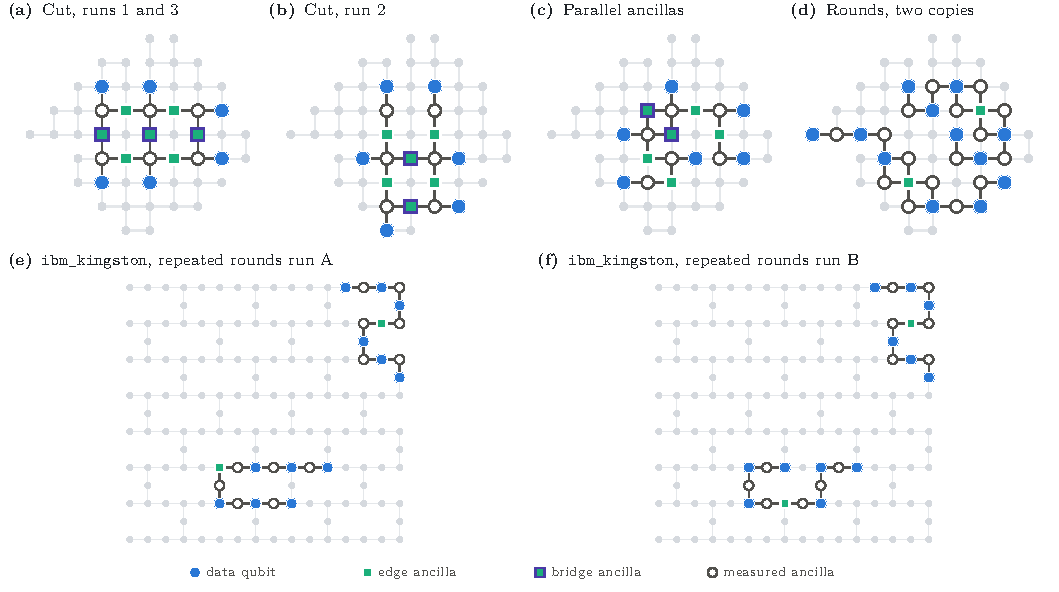
\includegraphics[width=\textwidth]{hardware_chips.pdf}
\caption{Placements on the chips.  Grey: unused qubits and couplers; dark
lines: the couplers that the submitted circuit uses.  (a)--(d)~IQM Emerald,
54 qubits, with the qubit numbers of the Open Quantum coupling map read from
zero (every placement is also SWAP-free when they are read from one).
(a)~Cut obstruction, width three, runs 1 and 3 (widths one and two use a
subset).  (b)~Run 2, width two (width one uses a subset).  (c)~Two parallel
ancillas on one bridge edge.  (d)~Repeated rounds, two copies of the circuit,
with the star and check ancillas of both rounds.
(e),~(f)~\texttt{ibm\_kingston}, heavy-hex lattice of 156 qubits, in the
repeated-rounds runs A and B: each run uses two 13-qubit paths, one for each
copy of the circuit.  The \texttt{ibm\_fez} cut-obstruction circuits
were routed by the transpiler and have no fixed placement.  The chip
coordinates are derived from the coupling maps.}
\label{fig:hardware-chips}
\end{figure*}

\paragraph{Checks before submission.}
Each circuit as submitted was checked to (i) on IQM, parse with Qiskit's
OpenQASM~3 importer and equal the reference circuit as a Clifford operation;
(ii) pass every detector with the correct observable in a noiseless
stabilizer simulation; (iii) have the stated exact circuit fault distance,
computed by the CP-SAT solver of \texttt{min\_weight\_logical.py} on the Stim
detector error model of the circuit with every operation noisy (and, in the
scheduled IBM repeated-rounds circuits, every idle window); and (iv) for the
IBM repeated-rounds circuits, use exactly the planned physical qubits and
pass the platform's instruction-set and timing validation.  For the run repeated on
the same IQM qubits, the platform's recorded input hashes confirm
byte-identical circuit files.

\paragraph{Analysis.}
Every result is the error of the observable after postselection on all
detectors, with Wilson 95\% intervals; comparisons use one-sided Fisher exact
tests (Table~\ref{tab:hardware-tests}).  For the later runs, marked P in that
table, the test and its level $0.05$ were fixed in the analysis script before
the jobs were submitted.  For the first runs the analysis code was fixed
before the data, but the tests were chosen afterwards.  The bit order of each
output is checked against the data wherever possible: on IQM the intended
order gives detector rates near the noise model and every other candidate
order gives rates near one half.  The IBM repeated-rounds circuits are
symmetric under reversal of the bit string, so there the documented order is
used; the \texttt{ibm\_fez} run confirmed it, since the reversed reading puts
every detector at one half.

\subsection{Cut obstruction}
\paragraph{Circuit.}
Each block is a three-qubit code with $Z$ checks $Z_0Z_1$ and $Z_1Z_2$,
$\overline X=X_0X_1X_2$ (a weight-three membrane, the stand-in for a slab
port) and $\overline Z=Z_0$.  The gauging graph has one vertex per data
qubit, the edges $(a_0,a_1)$, $(a_1,a_2)$, $(b_0,b_1)$, $(b_1,b_2)$, and the
bridge edges $(a_i,b_i)$ for $i<w$; an ancilla on every edge starts in
$|0\rangle$.  Each vertex star is measured once by its own ancilla, which is
read only at the end, so the circuit needs no mid-circuit measurement; at the
end every data and edge qubit is read in $Z$.  The blocks start in
$|000\rangle$, so the deformed $\overline Z_a\overline
Z_b=Z_{a_0}Z_{b_0}Z_{(a_0,b_0)}$ must read $+1$.  The detectors are the
deformed $Z$ checks $Z_xZ_yZ_{(x,y)}$ and, for $w\ge2$, the cycle checks of
the bridge squares.  By Proposition~\ref{prop:cut-obstruction}, $X$ on the
$w$ bridge edges is equivalent to $\overline X_a$, so the deformed $X$
distance is $w$, and the exact circuit fault distance is also $w$ for
$w=1,2,3$, both for the reference circuits and for the compiled IBM circuits.
On IQM the circuits use $16$, $18$ and $20$ CZ gates; on the heavy-hex
lattice of \texttt{ibm\_fez} the compiled circuits need \hwFezCZ{} CZ gates.

\paragraph{Results.}
Table~\ref{tab:hardware-cut} and Fig.~\ref{fig:hardware-sm}(a) give the data.
IQM runs 1 and 3 use one set of qubits; run 2 uses a set that shares 8 of its
19 qubits and none of its bridge qubits; run 3 repeats run 1 with
byte-identical files.  On both devices the error drops sharply from $w=1$ to
$w=2$ ($p\le\hwIQMpOneTwo$ in each IQM run with both widths,
$p=\hwIBMpOneTwo$ on IBM), and on
IBM again from $w=2$ to $w=3$ ($p=\hwIBMpTwoThree$).  On IQM width three had
no failure in \hwIQMwThreeKept{} kept samples, but width two was already so
rare there (\hwIQMwTwo\%, pooled) that the test fixed before run~3 was not met
($p=\hwIQMpTwoThree$).  The decoded error without postselection, a secondary
measure chosen afterwards, does fall from width two to width three, from
\hwDecTwo\% to \hwDecThree\% in run~3 ($p\le\hwDecP$ in runs 1 and 3).  The
control column shows that the cycle checks cause the gain: postselecting the
same samples on the block checks alone returns widths two and three to the
width-one level.  The IBM errors exceed the model, which assumed typical
published median error rates and no idle or crosstalk errors.

\subsection{Edge multiplicity}
\paragraph{Circuit.}
The width-one bridge edge $(a_0,b_0)$ carries two parallel ancillas, as in
Corollary~\ref{cor:edge-multiplicity} with $m=2$ on that edge.  The bundle
cycle $Z_eZ_{e'}$ of the two parallel edges is a new detector, so a single
$X$ fault on one of them is detected and the deformed $X$ distance is two.
On the square lattice the vertex ancillas of $a_0$ and $b_0$ share both
parallel edge qubits as neighbors, which fits the circuit on IQM without SWAP
gates.

\paragraph{Gate order.}
In the first version of the circuit each of the two vertex ancillas applied
its CNOTs to the two parallel edges one after the other.  The exact circuit
fault distance of that circuit is one: an $X$ fault on the vertex ancilla
just before these two CNOTs spreads to both parallel edges, which flips the
observable and leaves the bundle cycle silent.  Ordering each star as first
parallel edge, data qubit, second parallel edge, block edge makes every such
spread detectable, and the exact circuit fault distance becomes two.  This is
an instance of the constant $c_1$ of Sec.~\ref{sec:ft}, the number of
phenomenological mechanisms that one circuit fault can produce; with parallel
ancillas the extraction order decides whether that constant costs distance.

\paragraph{Results.}
With all checks the error is \hwMult\% (Table~\ref{tab:hardware-cut}),
against \hwIQMwOne\% for one bridge qubit in runs 1 and 2
($p=\hwMultP$); ignoring the bundle cycle gives \hwMultCtrl\%.  Two parallel
ancillas protect less than two separate bridge edges ($p=\hwMultVsTwoP$).
Both need two faults, but the parallel version has more two-fault paths, as
the noise model also predicts.

\subsection{Repeated rounds}
\paragraph{Circuit.}
The reported bit is the product of the vertex-star outcomes.  To test its
protection we use two three-qubit phase-flip blocks ($X$ checks $X_0X_1$,
$X_1X_2$; $\overline X=X_0$; $\overline Z=Z_0Z_1Z_2$, so $d_Z=3$) in
$|{+}{+}{+}\rangle$, so that $\overline X_a\overline X_b=+1$, joined by one
edge qubit $e$ in $|0\rangle$.  The stars $A_{a_0}=X_{a_0}X_e$ and
$A_{b_0}=X_{b_0}X_e$ are random individually, and their product
$X_{a_0}X_{b_0}$, the reported bit, must be $+1$.  In each of $R$ rounds the
two stars and the four block checks are measured with ancillas.  The
detectors are every block-check outcome and, from the second round on, every
star outcome against the previous round; the observable is the round-one
product.  A phase error on a port qubit flips one star in every round but
also a block check, so the bit is limited by $R$ and not by the toy code: the
exact circuit fault distance is $\min\{R,3\}$, that is $1$, $2$ and $3$ for
$R=1,2,3$ and still $3$ for $R=4$ (computed on the compiled IBM circuits), as
in Eq.~(A15s).

\paragraph{IQM: fresh ancillas.}
The IQM platform rejects any operation on a qubit after it has been measured,
so each round uses its own ancillas, all read at the end.  The edge qubit has
four couplers, which allows two rounds.  The error falls from \hwRndIQMOne\%
to \hwRndIQMTwo\% (Table~\ref{tab:hardware-rounds}; $p=\hwRndIQMp$, fixed in
advance), close to the model, and ignoring the round-to-round comparison
returns it to \hwRndIQMctrl\%.

\paragraph{IBM: measure and reset.}
On \texttt{ibm\_kingston} the ancillas are measured and reset between rounds.
Both steps, from $R=1$ to $2$ and from $2$ to $3$, are clear in two runs on
different days (every step $p\le\hwRndIBMmaxP$, fixed in advance), and
ignoring the round-to-round comparison returns the error to \hwRndIBMctrl\%.
The gain is, however, far below the calibrated model: \hwRndIBMTwo\% and
\hwRndIBMThree\% at $R=2,3$ in run A, against \hwRndIBMModelTwo\% and
\hwRndIBMModelThree\%.

\paragraph{Errors that survive the reset.}
The excess comes from ancilla errors that persist across rounds.  A check
ancilla that reads 1 in rounds 1 and 2 while the ancillas sharing its data
qubits show no change cannot be explained by a data error.  Independent
readout and gate errors would make this happen in about \hwPersIndep\% of
samples, but it happens in \hwPersSingle\% (run B, one reset;
Table~\ref{tab:hardware-rounds}).  On a star ancilla the same event repeats a
wrong outcome in every round, which no round-to-round comparison can see.
Run B tests whether failed resets cause it by applying two resets between
rounds, interleaved in time with the single-reset circuits on the same
qubits.  The second reset lowers the persistence only from \hwPersSingle\% to
\hwPersDouble\% (a \hwPersRel\% reduction, $p=\hwPersP$) and the error at
$R=3$ from \hwResetThreeS\% to \hwResetThreeD\% ($p=\hwResetThreeP$); at $R=2$
the change is not significant ($p=\hwResetTwoP$).  Most of the persistence is
therefore something that a reset cannot undo, most likely leakage out of the
computational subspace, which a measure-and-flip reset leaves in place.  The
IQM runs, whose ancillas are never reused, agree with their model.  A
persistent ancilla error is one physical event that produces faults in every
round, while the local-stochastic model of Sec.~\ref{sec:ft} bounds the
probability of faults in $R$ rounds by $p^R$; leakage reduction is the
hardware measure that makes such events rare enough for the model to apply.

\paragraph{No $R=4$ on hardware.}
For $R=4$ the exact circuit fault distance stays at $d_Z=3$, but the
calibrated model predicts an error far below what the available QPU time
could resolve, so the cap $\min\{R,d_Z\}$ is shown only by the exact
distance computation.

\subsection{Excluded runs}
Two earlier attempts used a 108-qubit Rigetti processor through Open Quantum.
In the first the compiler chose the placement; in the second the
cut-obstruction circuits were placed without SWAP gates and qubit rewiring was
disabled.  Both gave detector violation rates between about $0.2$ and $0.5$,
most of them near one half, and in the second one physical qubit read 1 in \hwStuck{} of 30{,}000 shots although
the platform listed it as operational.  The platform provides no calibration
data, so faulty qubits could not be avoided; both attempts are excluded from
the analysis, and their outputs and diagnosis are archived.  A probe of
mid-circuit measurement on IQM failed at execution, because an operation
followed a measurement, and returned no data.

\subsection{Files}
All hardware material is in the folder \texttt{hardware}.
\texttt{cut\_obstruction\_hw.py} defines the cut-obstruction circuits,
detectors, observable and lookup decoder, and submits and analyzes the
\texttt{ibm\_fez} run; \texttt{circuit\_distance\_check.py} computes their
exact circuit fault distances.  \texttt{embed\_iqm.py},
\texttt{export\_iqm.py} and \texttt{final\_check\_iqm.py} place, write and
check the IQM circuits, and \texttt{analyze\_iqm.py},
\texttt{cycle\_check\_control.py} and \texttt{analyze\_pooled\_w23.py} analyze
them.  \texttt{multiplicity\_hw.py}, \texttt{export\_multiplicity.py} and
\texttt{analyze\_multiplicity.py} do the same for the parallel-ancilla
circuit; \texttt{rounds\_hw.py}, \texttt{export\_rounds.py} and
\texttt{analyze\_rounds.py} for the IQM rounds; and
\texttt{ibm\_rounds\_hw.py}, \texttt{ibm\_rounds\_plan.py},
\texttt{ibm\_rounds\_submit.py}, \texttt{ibm\_rounds\_analyze.py},
\texttt{ibm\_rounds\_persistence.py} and the three \texttt{ibm3\_reset}
scripts for the IBM rounds.  The submitted circuits (\texttt{qasm3\_*.qasm},
\texttt{*.qpy}), the platform outputs (\texttt{oq\_*output*.json},
\texttt{hw\_counts.json}, \texttt{ibm2\_rounds\_bits.npz},
\texttt{ibm3\_reset\_bits.npz}), the job identifiers, the IBM calibration
snapshots and the Open Quantum backend descriptions are included.  The
submission helpers in \texttt{hardware/submission} read access keys from
files that are not part of the package.  \texttt{hardware\_summary.py}
recomputes every hardware number of the main text and of this section and
writes Tables~\ref{tab:hardware-cut}, \ref{tab:hardware-rounds}
and~\ref{tab:hardware-tests} and \texttt{hardware\_macros.tex};
\texttt{make\_hardware\_figure.py} draws the main-text hardware figure and
Figs.~\ref{fig:hardware-sm} and~\ref{fig:hardware-chips}.

\section{Space--time tradeoff and a concrete resource estimate}
\label{sec:resource-estimate}

\paragraph{The depth bound.}
Theorem~\ref{thm:A24} pairs the space bound $O(Wf+(B_f(A)+1)f^{3/2})$, which is
$O(Wf+f^{3/2})$ for a bounded-aspect box
(Corollary~\ref{cor:bounded-aspect-packing}), with the depth
bound $O(Tf^{3/2}\Psi)$, $\Psi=O(f^{\log_215})$, i.e.\ $O(Tf^{5.41})$ rounds.
This depth is the price of the minimal-space schedule: every data cell has
one depth-first factory, a distilled resource costs $O(\Psi)$ serialized
gadget slots of $O(f)$ rounds, and a logical layer waits for the $O(K)$
resources of its cell.  A logical layer of lattice surgery, by contrast,
takes $O(f)$ rounds.  The two schedules are the ends of one tradeoff.  With
$P$ factories per data cell ($1\le P\le K$), the space is
$O(WfP+f^{3/2})$ and the depth $O(TKf\Psi/P)$, so the qubit-time
$O(WTf^{5/2}\Psi)$ does not depend on $P$; the serial schedule minimizes
space, not qubit-time.  The exponent $\log_215$ comes from the quadratic
recursion $q_{r+1}\le C q_r^2$ proved for always-output distillation under
local-stochastic noise.  The standard cubic suppression of $15$-to-$1$
distillation would give $\Psi=O(f^{\log_315})=O(f^{2.47})$, but it is not
proved here for jointly local-stochastic inputs.

\paragraph{A concrete estimate.}
The theorem fixes exponents, not constants.  The script
\texttt{resource\_estimate.py} evaluates the accounting of
Theorem~\ref{thm:A24} with every constant stated as a named, adjustable
assumption (listed with its value in \nolinkurl{resource_estimate.md}).  Every
schedule receives an explicit integer allocation of blocks, or surface-code
tiles, by role: data, working slots, factories, and couriers.  Each schedule's
distance is chosen from its complete runtime, including the time spent
waiting for resources: $f$ is the least odd distance with
$L_{\rm live}R_{\rm total}\,p_L(f)\le\varepsilon/2$, where $L_{\rm live}$ counts
every live logical qubit, $R_{\rm total}$ is the runtime in rounds, and
$p_L(f)=0.1\,(p/p_{\rm th})^{(f+1)/2}$ with $p_{\rm th}=10^{-2}$ for both
architectures.  The final resources are budgeted separately,
$WT\,q_{\rm final}\le\varepsilon/2$.  The target is $W=100$ logical sites and
$T=10^6$ logical layers with one distilled $|A\rangle$ per site and layer, at
total failure $\varepsilon=10^{-2}$.

Three distillation models are kept separate.  (i) \emph{Proved}: the
always-output bound (A8), $q_{r+1}=C_{\rm dist}q_r^2$, with
$C_{\rm dist}=\binom{30}{2}=435$ on layer-code blocks (fifteen principal and
fifteen $S$-correction slots per run), and, as an assumed analog,
$\binom{15}{2}=105$ for a surface-code unit, whose rotations need no
$|Y\rangle$ correction (Lemmas~\ref{lem:A5} and~\ref{lem:A7} are proved for
the factory (A4a), not for that unit).
(ii) \emph{Exact}: the exact error map of the ideal always-output factories
for independent $Z$-type candidate errors, from an enumeration of all
$2^{15}$ patterns.  Every pair of errors is malignant (the syndrome of a pair
is that of a third coordinate, and the three form a weight-three logical), so
$q_{\rm out}=105q_c^2-1330q_c^3+O(q_c^4)$; on layer-code blocks the
per-coordinate error $q_c=q_A+q_Y/2-q_Aq_Y$ includes the $S$ correction, used
with probability one half.  (iii) \emph{Postselected}: standard $15$-to-$1$
and $7$-to-$1$ distillation that discards nontrivial syndromes
($q_{\rm out}=35q^3+O(q^4)$, with retries).  The theorem does not cover this
model.  A $15$-to-$1$ run on layer-code blocks takes $30$ gadget slots of $3f$
rounds and consumes fifteen $S$-correction resources assigned in the fixed
schedule and produced just in time, themselves distilled by $7$-to-$1$ runs
of $14$ slots; a raw resource costs two slots of
injection and courier transfer.

The layer-code block is the explicit realization at $s=2$ of a balanced input
with rate $0.1$, relative distance $0.1$, check weight $8$, and supports
spanning the input.  Its size $n$ follows from the Euler count of
Proposition~\ref{prop:explicit-k} and $K=\lfloor0.1N\rfloor$.  Its distance is
bracketed by Theorem~\ref{thm:explicit-distance} between
$L_z\lceil d^{\rm in}/4\rceil$ and $L_zd^{\rm in}+s\,m_Xn_{\rm in}$.  The
estimate uses the ratio $d=L_zd^{\rm in}/2$ of the exact small instances and
reports two further scenarios in \nolinkurl{resource_estimate.md}: the proved
lower bound, and the data-string part $L_zd^{\rm in}$ of a slab (not a proved
upper bound).  A data block holds $K-1$
data sites and one working slot (one site and a separate working block when
$K=1$).  The theorem's serial schedule gives each data block a depth-first
factory of $15\ell+7(\ell-1)+2$ logical slots and two live courier blocks; a
shared serial schedule uses one such factory for all data blocks, as a
surface-code layout with one factory unit does; and a throughput-limited
schedule runs factories in parallel so that each logical layer takes two
gadget slots.  Every block carries one extraction ancilla per qubit and a
gauging grid of multiplicity two, and an extraction round has $28$ CNOT
layers.  For the surface code we use $2d^2$ qubits per tile, two tiles per
logical site, a logical layer of $2d$ rounds, $15$-to-$1$ units of $11$ tiles
for $11d$ rounds, and $8$ layers per round.  One layer is taken to last
$50$\,ns.

\begin{table*}[t]
\caption{Resource estimate for $W=100$, $T=10^6$, $\varepsilon=10^{-2}$, with
explicit integer allocations and distances chosen from each schedule's
complete runtime (\texttt{resource\_estimate.py}).  Upper block: $p=10^{-3}$,
injected error $q_0=10^{-2}$, where only the postselected factory (not
covered by the theorem) converges on layer-code blocks.  Lower block:
$p=10^{-4}$, $q_0=10^{-3}$, with the always-output bound (A8) (an assumed
analog for the surface-code unit).  ``Serial''
gives each data block its own factory, as in Theorem~\ref{thm:A24}; ``shared''
uses one factory for all data blocks; ``throughput'' adds factories until a
logical layer takes two gadget slots (layer code) or $2d$ rounds (surface
code).  All constants are stated assumptions; the table is not a hardware
prediction.}
\label{tab:resource-assumptions}
\centering
\small
\setlength{\tabcolsep}{6pt}
\begin{tabular}{@{}llrrrrrrr@{}}
\toprule
Architecture & Schedule & levels & $f$ & block $n$ & $K$ & peak qubits & wall time & qubit-seconds \\
\midrule
\multicolumn{9}{@{}l}{$p=10^{-3}$, $q_0=10^{-2}$, postselected distillation}\\
Layer code & serial & 3 & 35 & $7.6\times10^{4}$ & 2 & $1.0\times10^{9}$ & 61 d & $5.5\times10^{15}$ \\
Layer code & shared & 3 & 37 & $9.8\times10^{4}$ & 2 & $5.2\times10^{7}$ & 18 yr & $2.9\times10^{16}$ \\
Layer code & throughput & 3 & 33 & $5.8\times10^{4}$ & 2 & $1.8\times10^{12}$ & 282 s & $4.9\times10^{14}$ \\
Surface code & serial & 2 & 31 & $1922$ & 1 & $4.1\times10^{5}$ & 2.9 d & $1.0\times10^{11}$ \\
Surface code & throughput & 2 & 29 & $1682$ & 1 & $1.9\times10^{8}$ & 23 s & $4.4\times10^{9}$ \\
\midrule
\multicolumn{9}{@{}l}{$p=10^{-4}$, $q_0=10^{-3}$, always-output bound (A8)}\\
Layer code & serial & 5 & 19 & $4.1\times10^{4}$ & 1 & $1.8\times10^{9}$ & 18 yr & $1.0\times10^{18}$ \\
Layer code & shared & 5 & 21 & $4.6\times10^{4}$ & 2 & $2.8\times10^{7}$ & $2\times10^3$ yr & $1.8\times10^{18}$ \\
Layer code & throughput & 5 & 19 & $4.1\times10^{4}$ & 1 & $4.0\times10^{14}$ & 741 s & $3.0\times10^{17}$ \\
Surface code & serial & 4 & 17 & $578$ & 1 & $1.2\times10^{5}$ & 313 d & $3.3\times10^{12}$ \\
Surface code & throughput & 4 & 17 & $578$ & 1 & $1.3\times10^{10}$ & 14 s & $1.7\times10^{11}$ \\
\bottomrule
\end{tabular}
\end{table*}

\paragraph{What the estimate shows.}
Three conclusions hold for all three distance scenarios in
\nolinkurl{resource_estimate.md}.  First, distillation.  At $p=10^{-3}$ with
injected error $q_0=10^{-2}$, neither always-output model converges on
layer-code blocks: the proved recursion needs $q_0<1/435\approx2.3\times10^{-3}$,
and the exact map of the ideal factory, with same-level $S$ corrections,
needs $q_0<4.7\times10^{-3}$ ($1.1\times10^{-2}$ without corrections).  The
postselected factory converges up to $q_0\approx8\times10^{-2}$, so the
comparison at this noise point uses it for both architectures.  At $p=10^{-4}$
and $q_0=10^{-3}$ all three models converge, in five, four and two levels on
layer-code blocks.  Second, the block.  At the distances needed here
($f\approx15$--$37$) a block of this family holds one to three logical
qubits ($8\times10^3$ to $3\times10^5$ qubits per block across the scenarios),
so it stores one or two data sites.  With the same accounting as the tables
(extraction ancillas and gauging grid for the layer code, a routing tile for
the surface code), a layer-code block stores a logical more cheaply than two
surface-code tiles from $d=1103$, and for every larger tabulated distance from
$d=1169$; the corresponding values are $609$ for the data-string scenario and
$2000$ (stably from $2309$) for the proved lower bound, where a block holds
$15$ ($8$, $28$) logical qubits.  Comparing a bare block with extraction
ancillas against a single tile gives the same distances.  Third, space and time.
At these distances the layer code loses to the surface-code baseline in peak
space, in wall time, and in qubit-time; the qubit-time gap is $4.7$ to $6.2$
orders of magnitude for the rows of Table~\ref{tab:resource-assumptions} (three
to six across all models and scenarios), because each factory run occupies whole blocks for $30$
gadget slots and each $15$-to-$1$ run also consumes fifteen distilled
$|Y\rangle$ corrections.

Four changes would move these numbers most: inputs whose blocks carry many
logical qubits already at moderate distance; factories that do not tie up a
whole block per gadget, or distillation delegated to a different code with a
protected local transfer; an always-output protocol with cubic suppression
under local-stochastic noise; and a lower raw injection error.  The
asymptotic advantage of the architecture is real, but the present constants
place it far from the practical regime.  (The superseded estimate of an
earlier version, and the audit that reproduces its errors, are recorded in
Sec.~\ref{sec:archive}.)


\section{Symplectic-overlap extensions and benchmarks}
\label{sec:supp-overlap}
The following consequences of the overlap-corrected cleaning theorem are independent of the fault-tolerance proof.  Besides pairwise overlap benchmarks, they expose a two-polarization mobility tradeoff linking rate, distance, disjointness, and shallow logical gates.

\subsection{Hierarchy and arbitrary stabilizer codes}
Using the CSS notation of the detailed overlap section, one may refine the invariant to
\begin{equation}
 \chi_r^{XZ}(Q)=\min_{A,B:\,r(A,B)\ge r}|A\cap B|,
 \qquad 1\le r\le K. \tag{S12}
\end{equation}
The rank-factorization argument in the detailed overlap theorem implies immediately
\begin{equation}
 \chi_r^{XZ}(Q)\ge r. \tag{S13}
\end{equation}
This hierarchy records how much physical intersection is required to carry
$r$ independent dual logical commutators, rather than how much support is
required for an $r$-dimensional subcode.
The detailed port-packing theorem is the corresponding many-port statement: summing the overlap inequality over regions of bounded physical multiplicity gives $\sum_i g_X(A_i)\le c|B|$ whenever $B$ supports all pure-$Z$ logical classes.  The preceding analysis also gives a direct injectivity proof of the complete-$B$ case.

There is also a general stabilizer version with a sharp factor of two.  Let
$\mathcal L=S^\perp/S$ be the $2K$-dimensional logical symplectic space of an
$[[n,K]]$ stabilizer code and choose complementary logical Lagrangians
$\mathcal L=U\oplus W$, $\dim U=\dim W=K$.  Suppose region $A$ supports all
classes in $U$ and region $B$ supports all classes in $W$.  If
$C=A\cap B$ has $m$ qubits, choose linear supported representative maps
$\sigma_U:U\to S^\perp\cap V_A$ and
$\sigma_W:W\to S^\perp\cap V_B$.  All cross commutation occurs in $C$, so
\begin{equation}
 \omega_{\mathcal L}(u,w)
 =\omega_C\!\left(\sigma_U(u)|_C,\sigma_W(w)|_C\right). \tag{S14}
\end{equation}
The perfect rank-$K$ logical pairing therefore factors through
$V_C\cong\mathbb F_2^{2m}$, which gives
\begin{equation}
 K\le2m,\qquad |A\cap B|\ge\lceil K/2\rceil. \tag{S15}
\end{equation}
The factor two is sharp.  For the $[[3,2,1]]$ code
$S=\langle X_1X_2X_3\rangle$, take $A=\{1,2\}$ and $B=\{2,3\}$ and the two
commuting logical Lagrangians
\begin{align*}
 U&=\operatorname{span}\{X_1X_2,\,Z_1Z_2\},\\
 W&=\operatorname{span}\{Z_2Z_3,\,X_2X_3\}.
\end{align*}
Their cross-pairing matrix is $I_2$, while $|A\cap B|=1$ and $K=2$.
The stronger CSS bound arises because a pure-$X$ restriction on $m$ qubits
lives in an $m$-dimensional binary space rather than the full $2m$-dimensional
local Pauli symplectic space.

\subsection{Symplectic rederivation of the BPT tradeoff}
The geometric part of the Bravyi--Poulin--Terhal (BPT) argument partitions a
$D$-dimensional local code into
\begin{equation}
 \Lambda=R_1\sqcup R_2\sqcup C, \tag{S16}
\end{equation}
where $R_1$ and $R_2$ are correctable and, for a block scale $R$ chosen with
$R^{D-1}=\Omega(d)$, the separator obeys
\begin{equation}
 |C|=O(n/R^2)=O\!\left(n/d^{2/(D-1)}\right)
 \tag{S17}
\end{equation}
\cite{BPT}.  For a CSS stabilizer code, correctability of $R_1$ lets every
pure-$X$ logical be cleaned into $A=R_1^c$, and correctability of $R_2$ lets
every pure-$Z$ logical be cleaned into $B=R_2^c$; this is the standard cleaning
mechanism \cite{HaahPreskillTradeoff}.  Since
\begin{equation}
 A\cap B=(R_1\cup R_2)^c=C, \tag{S18}
\end{equation}
the detailed universal bound $\chi_{XZ}\ge K$ gives the sandwich
\begin{equation}
 K\le\chi_{XZ}(Q)\le O\!\left(n/d^{2/(D-1)}\right), \tag{S19}
\end{equation}
and hence
\begin{equation}
 Kd^{2/(D-1)}=O(n). \tag{S20}
\end{equation}
Thus the standard BPT geometry can be combined with the overlap rank theorem
to give a purely symplectic rederivation of the stabilizer/CSS scaling law.
The geometric construction is BPT's; the new point here is the interpretation
of its separator as a carrier of the logical $X/Z$ commutation rank.  This
argument is inherently Pauli/stabilizer and does not extend the original BPT
result for more general local commuting-projector codes.

For the present three-dimensional layer codes,
$n=\Theta(N^3)$, $d=\Theta(N^2)$, and $K=\Theta(N)$, so both ends of (S19)
scale as $\Theta(N)$.  Their native transverse slabs therefore attain the
algebraic lower scale and the three-dimensional BPT upper scale
simultaneously:
\begin{equation}
 \chi_{XZ}=\Theta(K)=\Theta(n/d). \tag{S21}
\end{equation}

\subsection{Price as the union analog}
Pastawski and Preskill define the price $p(Q)$ as the minimum number of
physical qubits in a region supporting the complete logical algebra and prove
the strong quantum Singleton bound
\begin{equation}
 p(Q)-K\ge d-1 \tag{S22}
\end{equation}
for subspace codes \cite{PastawskiPreskillPrice}.  For the same feasible CSS
pairs used in the definition of $\chi_{XZ}$,
\begin{equation}
 p(Q)=\min_{\substack{A,B:\\g_X(A)=K,\;g_Z(B)=K}}|A\cup B|. \tag{S23}
\end{equation}
Indeed, $A\cup B$ supports the product of any pure-$X$ and pure-$Z$ logical
representatives and hence the full logical Pauli algebra, while an optimal
price region $R$ gives the feasible choice $A=B=R$.

Consequently, for every feasible pair,
\begin{align*}
 |A\cup B|&\ge d+K-1,\\
 |A\cap B|&\ge K,
\end{align*}
and therefore
\begin{equation}
 |A|+|B|\ge d+2K-1. \tag{S24}
\end{equation}
For the native layer-code slabs, bounded density gives
$|A\cup B|=O(N^2)=O(d)$ while the detailed layer-code overlap corollary gives $|A\cap B|=\Theta(K)$.  Equation~(S22)
then supplies the matching union lower bound, so the same transverse pair is
simultaneously efficient in the two complementary senses
\begin{equation}
 (|A\cup B|,|A\cap B|)=(\Theta(d),\Theta(K)). \tag{S25}
\end{equation}
This yields the dimensional hierarchy
\begin{equation}
\begin{aligned}
 \Theta(n)&:\ \text{bulk volume},\\
 \Theta(d)&:\ \text{complete-logical interface},\\
 \Theta(K)&:\ \text{symplectic intersection}.
\end{aligned}\tag{S26}
\end{equation}

\subsection{Bipolar mobility, price, and the crossbar corner}
Let $A_1,\ldots,A_r$ be pairwise-disjoint complete pure-$X$ ports and
$B_1,\ldots,B_s$ pairwise-disjoint complete pure-$Z$ ports of an $[[n,K]]$
CSS code.  The detailed symplectic-crossbar theorem gives
\begin{equation}
 rsK\le n. \tag{S27}
\end{equation}
The price relation also constrains the same two families.  Applying (S24) to
every pair $(A_i,B_j)$ and summing gives
\begin{align*}
 rs(d+2K-1)
 &\le \sum_{i,j}(|A_i|+|B_j|)\\
 &=s\sum_i|A_i|+r\sum_j|B_j|\\
 &\le (r+s)n,
\end{align*}
so
\begin{equation}
 rs(d+2K-1)\le(r+s)n. \tag{S28}
\end{equation}
For balanced bipolar mobility $r=s=m$, Eqs.~(S27)--(S28) become
\begin{equation}
 n\ge\max\!\left\{m^2K,\;\frac m2(d+2K-1)\right\}. \tag{S29}
\end{equation}
In particular, if $R=K/n$ then $Rm^2\le1$.  If $m=\Omega(K)$, any such CSS
family requires $n=\Omega(K^3)$.  The balanced layer-code family has
$m=\Theta(K)$ and $n=\Theta(K^3)$, so it saturates this physical-qubit lower
bound up to constants.

The scaling can be summarized by exponents.  Suppose
$K=n^{\alpha+o(1)}$, $d=n^{\beta+o(1)}$, and
$m=n^{\mu+o(1)}$.  The crossbar bound, the balanced price bound, and the
three-dimensional BPT bound respectively imply
\begin{equation}
 2\mu+\alpha\le1,\qquad
 \mu+\max\{\alpha,\beta\}\le1,\qquad
 \alpha+\beta\le1. \tag{S30}
\end{equation}
If all three inequalities are saturated and $\mu>0$, the only possible
triple is
\begin{equation}
 (\alpha,\beta,\mu)=\left(\frac13,\frac23,\frac13\right). \tag{S31}
\end{equation}
Indeed, the first and third equalities give $\mu=\beta/2$.  If
$\beta\ge\alpha$, saturation of the middle inequality gives
$3\beta/2=1$ and hence (S31).  If $\alpha\ge\beta$, the same equations force
$\beta=\mu=0$, excluded by $\mu>0$.  Thus the layer-code exponents form the
unique nontrivial simultaneous-saturation corner of these three constraints.

There is a parallel gate-theoretic consequence.  Put $m=\min\{r,s\}$.  For
any nontrivial logical Pauli coset $G=[X(u)Z(v)]$, choose the $i$th pure-$X$
and pure-$Z$ representatives and multiply them.  Pairwise disjointness within
each polarization makes these $m$ representatives $2$-disjoint, exactly as
in the detailed layer-code argument.  Hence
\begin{equation}
 \Delta(Q)\ge m/2. \tag{S32}
\end{equation}
If $d_\uparrow/d_\downarrow$ remains bounded while $m\to\infty$, the
Jochym-O'Connor--Kubica--Yoder hierarchy criterion therefore excludes
bounded-arity fixed-depth non-Clifford code-preserving unitary gates for all
sufficiently large codes.  Bipolar mobility is thus simultaneously a
resource for local logical access and a source of static shallow-unitary
rigidity.

\subsection{Related boundary localization in tile codes}
A recent independent result for two-dimensional tile codes proves, under its
stated topological-order assumptions, a canonical symplectic basis with
$X$- and $Z$-logical operators supported in transverse boundary strips and
logical pairs labeled by physical qubits in their $D\times D$ corner overlap
\cite{BreuckmannTileLogical2026}.  For a fixed tile rule this is the two-dimensional
analog of a bulk $\to$ boundary-interface $\to$ transverse-overlap picture.
We do not infer the layer-code theorem from the tile-code construction (or
vice versa); the comparison only indicates that localized transverse logical
polarizations occur in more than one geometrically local CSS family.


\section{Uniform-gap mobility and disjointness checks}
\label{sec:supp-disjointness}
Two facts remove any dependence of the shallow-unitary corollary on a privileged slab.

\subsection{Why the prefix construction is gap-uniform}
In the explicit realization of Sec.~\ref{sec:explicit-realization} the slab
operators of Theorem~\ref{thm:slab-resolved} exist at every height $z_0$ and
every column $x_0$: the gluing forms of item~(1) of that theorem do not
depend on the coordinate, because every junction and wall rule adds qubits
that the slab operators do not use.  In particular no admissibility condition
is needed, and the prefix equations
\begin{equation}
 p_i=\sum_{h\le i}x_h,\qquad p_{i-1}+p_i+x_i=0 \tag{S33}
\end{equation}
are the same at every height.  The certificate of Sec.~\ref{sec:certificate}
checks this at every height and column of every tested code.  Hence
\begin{equation}
 r_X=L_z=\Theta(N),\qquad r_Z=L_x+1=\Theta(N) \tag{S34}
\end{equation}
disjoint complete ports exist for balanced inputs (Corollary~\ref{cor:uniform-gap-slabs}).

\subsection{Mixed logical Paulis and two-disjointness}
Let $G=[X(u)Z(v)]$ be any nontrivial logical Pauli coset and set
$r=\min(r_X,r_Z)$.  Choose $X_i(u)$ and $Z_i(v)$ in the $i$th slabs and set
$P_i=X_i(u)Z_i(v)$.  Since the $X$ slabs are mutually disjoint, a physical
qubit occurs in at most one $X_i$; the same is true of the $Z_i$.  Therefore
\begin{equation}
 \#\{i:q\in\operatorname{supp}P_i\}\le2 \tag{S35}
\end{equation}
for every physical qubit $q$.  These representatives are distinct.  If both
polarizations are nontrivial and $P_i=P_j$ up to phase, uniqueness of the
binary Pauli decomposition would make the pure-$X$ operator $X_iX_j$ equal a
pure-$Z$ operator $Z_iZ_j$, forcing both to be identity; pairwise disjoint
nonempty same-polarization supports exclude this for $i\ne j$.  The pure cases
are immediate.  Thus every $G$ has a $2$-disjoint set of size $r$, and the
single-qubit-partition disjointness obeys
\begin{equation}
 \Delta\ge r/2=\Omega(N). \tag{S36}
\end{equation}
Lemma~2 of Jochym-O'Connor, Kubica, and Yoder gives
$\Delta\le n_{\rm phys}/d_\uparrow$ \cite{JochymDisjointness}.  The fixed
transverse slab pair represents every mixed logical Pauli in $O(N^2)$ qubits,
whereas the ordinary layer-code distance is $\Theta(N^2)$; hence
\begin{equation}
 d_\downarrow=\Theta(N^2),\qquad d_\uparrow=\Theta(N^2),\qquad
 \Delta=\Theta(N). \tag{S37}
\end{equation}

\subsection{Exact scope of the shallow-unitary corollary}
For a $q$-local depth-$h$ physical unitary circuit, Theorem~9 of Ref.~\cite{JochymDisjointness}
shows that the induced logical unitary belongs to level $M$ of the Clifford
hierarchy if
\begin{equation}
 d_\uparrow q^{(2^M-1)h}<d_\downarrow\Delta^{M-1}. \tag{S38}
\end{equation}
At $M=2$ and fixed $q,h$, Eq.~(S37) makes the left-to-right ratio
$O(N^{-1})$.  Thus sufficiently large blocks are Clifford-only under such
static bounded-arity constant-depth unitary circuits, including transversal
circuits.  This is stronger for this family than the generic three-dimensional
Bravyi--K\"onig geometric-locality restriction, which allows the third level
of the Clifford hierarchy \cite{BravyiKoenig}.

The scope distinction is essential.  The theorem does not prohibit the
architecture in the companion manuscript because that construction uses protected
logical Pauli measurements, encoded resource states, classical feed-forward,
ancilla systems, and time-dependent code deformation.  These operations are
not a single bounded-depth unitary circuit preserving one fixed layer-code
codespace.


\section{Related architectures and implementation directions}\label{sec:related-extended}
The construction complements gauging \cite{WilliamsonYoderGauging}, parallel and parsimonious surgery \cite{CowtanParallelSurgery,YuanParsimonious2026}, homological measurement \cite{IdeHomological}, adapters and extractors \cite{SwaroopAdapters,HeExtractors}, lifted surgery \cite{BerentLiftedSurgery}, and recent universal good-qLDPC architectures \cite{ZhangGoodQLDPC,MalcolmEfficientQLDPC}.  Recent layer-code work also studies partial self-correction, random layer codes, weight reduction, and non-CSS embeddings \cite{WilliamsonPartialSelfCorrection2025,GuRandomLayerCodes2026,YuanBaspinWeightReduction2026,YuanBaspinNonCSS2026}.  Constant-overhead fault tolerance with LDPC codes \cite{GottesmanFTThreshold,KovalevPryadko,FawziGrospellierLeverrier} and magic-state injection into LDPC codes \cite{ZhangInjectionIndependence,LiuInSituInjection} use nonlocal connectivity.  Geometrically local approaches include surface-code lattice surgery \cite{HorsmanLatticeSurgery,LitinskiSurgery}, three-dimensional surface codes with transversal gates \cite{VasmerBrowne}, local simulation of LDPC codes \cite{PattisonHierarchical}, local fault-tolerance constructions \cite{ChoeKoenigLocal}, wire codes \cite{BaspinWire}, and planar logical measurements \cite{YangPlanar}.  The distinction relevant here is one sentence: universal fault-tolerant processing is carried out on a native three-dimensional Euclidean nearest-neighbor layer-code lattice (the explicit realization of the Williamson--Baspin defect network), with no nonlocal auxiliary connectivity.  Table~\ref{tab:comparison} gives a compact comparison.

\begin{table*}[t]
\caption{Compact positioning against selected related constructions.  The table describes each cited construction itself, not every capability that could be obtained by combining separate schemes.}
\label{tab:comparison}
\scriptsize
\setlength{\tabcolsep}{4.2pt}
\renewcommand{\arraystretch}{1.14}
\begin{tabular}{@{}p{2.35cm}p{3.0cm}p{3.65cm}p{2.75cm}p{4.3cm}@{}}
\toprule
Work & Geometry & Logical-operation mechanism & End-to-end circuit FT? & Principal resource scaling / emphasis \\
\midrule
Williamson--Yoder \cite{WilliamsonYoderGauging} & General code plus auxiliary gauging graph & Gauging an arbitrary logical Pauli & Spacetime fault-distance theorem for the gauging primitive & Ancilla overhead near-linear in logical weight up to polylogarithmic factors \\
Parallel / parsimonious surgery \cite{CowtanParallelSurgery,YuanParsimonious2026} & General sparse stabilizer connectivity & Parallel logical Pauli measurements via surgery & Fault-distance-preserving measurement framework & Parallel measurements; parsimonious ancilla systems of $O(w\log w)$ qubits for weight-$w$ logical Paulis \\
Homological measurement \cite{IdeHomological} & General CSS-code geometry & Edge-expanded / homological measurement & Distance-preserving logical-measurement framework & Ancilla count linear in logical weight for the edge-expanded protocol \\
Extractors \cite{HeExtractors} & Fixed sparse qLDPC connectivity & Extractor systems / Pauli-based computation & Universal PBC architecture, with high-fidelity non-Clifford supply as an interface & $\widetilde O(n)$ extractor size; logical cycles scale with syndrome rounds \\
Good-qLDPC architectures \cite{ZhangGoodQLDPC,MalcolmEfficientQLDPC} & General good-qLDPC or SHYPS connectivity & Parallel surgery/state preparation or transversal/fold-transversal Clifford processing & Universal or universal-completable FT architectures & Constant/low qubit overhead and reduced logical time in their respective settings \\
Lattice surgery \cite{HorsmanLatticeSurgery,LitinskiSurgery} & 2D nearest-neighbor surface-code patches & Merging and splitting patch boundaries & Standard surface-code fault tolerance & $\Theta(d^2)$ physical qubits per logical qubit \\
This work & 3D Euclidean nearest-neighbor layer-code lattice & Constant-width slabs + thick local 3D grid gauging + encoded courier & Scheduled-circuit distance and resource theorem; full distance kept in every measurement & $\Theta(f)$ qubits per logical, $O(Wf+(B_f(A)+1)f^{3/2})$ space; $O(Tf^{3/2}\Psi)$ depth with $\Psi=O(f^{\log_215})$ (see Sec.~\ref{sec:resource-estimate} for constants) \\
\bottomrule
\end{tabular}
\end{table*}


\subsection{Algorithmic and noise-model outlook}
\label{sec:decoder-noise}
\paragraph{Practical two-pass decoder.}
For algorithmic and numerical exploration, one may decode a layer-code block by (i) running a local decoder independently on each surface-code sheet, (ii) resolving the residual syndrome along the $O(1)$-width junction corridors by matching or belief propagation, and (iii) applying OSD only on the $O(1)$-width slab regions needed to settle the logical frame.  A positive-threshold proof for this decoder would require a separate cluster-expansion analysis of the residual failures, and a near-linear runtime claim would require an implementation and complexity analysis.  Neither is claimed here.  The theorem of Sec.~\ref{sec:ft} continues to use committed minimum-weight decoding.

\paragraph{Next numerical and algorithmic steps.}
Four directions follow from the present results.  (i) \emph{A growing family
of the explicit realization.}  The layer-code tests here vary the spacing of
small inputs up to $s=5$ (Sec.~\ref{sec:two-block-scaling}) and, with the
routed schedule, the input up to seven qubits
(Sec.~\ref{sec:two-block-routed}); neither probes $K=\Theta(N)$ and
$d=\Theta(N^2)$.  The next campaign should grow the input into that regime,
carry the multiplicity of Corollary~\ref{cor:edge-multiplicity} where the
grid's crossing number falls below the block distance, and shorten the routed
schedule, whose long idle periods leave the present sampled rates
uninformative, so that failure rates can be measured with a decoder close to
minimum weight.  (ii) \emph{A decoder
for deformation histories.}  The layer-code decoders of
Ref.~\cite{GuRandomLayerCodes2026} are a natural starting point, but changing
checks, inherited frames and records at cuts, and joint measurements require
new work.  (iii) \emph{Parallel access.}  How many logical measurements can
share the slab interfaces while keeping bounded congestion and full distance,
compared with parallel code surgery~\cite{CowtanParallelSurgery} under the
additional restriction of three-dimensional Euclidean locality?
(iv) \emph{Resource supply.}  Specialized factories that deliver resources to
layer-code data blocks through a protected local transfer would remove the
dominant cost identified in Sec.~\ref{sec:resource-estimate}.

\paragraph{Constructivity of the component codes.}
Leverrier--Z\'emor's random-method result is sufficient for the existential input family used in Lemma~\ref{lem:tanner-dense}.  A deterministic version would require component codes satisfying the needed distance and robustness conditions, or a derandomization that controls the global robustness predicate.  Limited-independence or conditional-expectation methods become applicable only after the relevant bad events and independence requirements are identified.  Random layer codes built from random CSS inputs \cite{GuRandomLayerCodes2026}, suggested by D.~J. Williamson (private communication), are a different route; the slab construction applies to the explicit realization of any CSS input, but the resource accounting would have to be redone with their parameter scaling.

\paragraph{Noise beyond local-stochastic Paulis.}
Randomized compiling and Pauli/Clifford twirling can tailor suitable Markovian noise toward stochastic Pauli descriptions under additional assumptions \cite{WallmanEmerson,BealeTwirl}, while leakage-reduction gadgets can return population to the computational subspace at additional local circuit cost \cite{SucharaLeakage}.  Extending the theorem requires a separate fault-path analysis for coherent temporal correlations, gate dependence, leakage propagation, and the interaction between leakage-reduction units and the detector schedule.  The exploratory probes of Sec.~\ref{sec:supp-negative} are diagnostics only.


\section{Archive: revision record and superseded material}
\label{sec:archive}
This section records what changed in successive revisions and keeps the
certificates and arguments that those revisions superseded, so that earlier
versions remain traceable.  Nothing in this section is used by the results
of Secs.~\ref{sec:slab}--\ref{sec:related-extended}.

\subsection{Revision of 14 October 2026}
Added the hardware demonstrations of Sec.~\ref{sec:hardware}, a main-text
section and figure that summarize them, a summary in the abstract and the
introduction, the corresponding acknowledgments, and the Open Quantum
citation~\cite{OpenQuantum2026}.  The main-text figure shows what was run
next to what was measured; Fig.~\ref{fig:hardware-sm} shows every run and
Fig.~\ref{fig:hardware-chips} every placement.  In the main text, the
surface-code threshold figure moved to this supplement
(Fig.~\ref{fig:supp-continuous}, same data), and a figure of the two-block
measurement on layer-code blocks took its place.  The runs found two practical points,
discussed in Sec.~\ref{sec:hardware} and in the main-text Discussion: the CNOT
order inside a vertex star decides
whether parallel ancillas keep their distance at circuit level, and ancilla
errors that survive a reset limit repeated rounds on hardware.  No
theoretical result changed.

\subsection{Revision of 9 October 2026}
An audit of the 8 October revision accepted the invariants (I1)--(I3) for the
abstract schedule but noted that no executable trace showed them for births,
cell reuse and adaptive branches, and that the hypothesis
$R_{\rm pad}(B)>\tau$ of Lemma~\ref{lem:primitive-paths} needed an explicit
parameter choice.  The choices $d_0>\tau$ and $R>\tau$ are now stated with
the courier estimate and Eq.~(A19), and \texttt{schedule\_verifier.py}
exports a complete schedule and checks it, with nine negative controls
(paragraph ``An executable schedule certificate'').  The audit also found that
the coordinates of the routing sketch \texttt{factory\_3d\_routing\_coords.csv}
overlap; that file is schematic and is now marked as such.

\subsection{Revision of 8 October 2026}
\paragraph{Rectangle distance without cleaning.}
The relative rectangle bound (Lemma~\ref{lem:relative-rectangle-distance})
previously rested on the cleaning interface of
Proposition~\ref{prop:cleaning-interface}, whose weight step WY6 was argued
by a timeline-parity sweep across entry, exit and idle boundaries.  A reader
asked for that step to be checked at every boundary.  It is now replaced by
the direct slice argument of Proposition~\ref{prop:slice-bound}, which needs
no sweep: the $X$-type faults leave one deformed logical at the right cut,
the $Z$-type faults leave a logical at the right cut or, in a round without a
record fault, an operator anticommuting with the measured logical, and in
each case every qubit of that operator carries a fault.  The bound is
slightly sharper, $\min\{\widetilde d_X,d_Z,R\}$, and
\texttt{rectangle\_slice\_check.py} shows by exact minimization that it is
attained (Table~\ref{tab:slice-check}).  Lemmas~\ref{lem:raw-quotient-distance}
and~\ref{lem:courier-spectators} now use the same argument with effects
recorded modulo the resource subgroup.

\paragraph{Separation of resource neighborhoods.}
Lemma~\ref{lem:resource-separation} previously derived the linking length
$\rho\geq\kappa R$ from a bounded-degree coloring of conflicting event cores,
which did not explicitly exclude paths through intermediate cells.  The
schedule invariants (I1)--(I3) are now stated, and
Lemma~\ref{lem:primitive-paths} shows that any path between the regions of
two primitives stays on one block for that block's whole padding; the
separation follows with $\kappa=1/\tau$ for every schedule satisfying the
invariants.  The same lemma closes a gap in the proof of
Theorem~\ref{thm:padded-protected-composition}, which inferred from the
temporal span of a short component alone that it meets at most one
primitive; that inference did not cover two primitives running at the same
time on disjoint blocks.

\subsection{Revision of 26 September 2026}
\paragraph{Boundary composition.}
The earlier worked gluing example wrote the T0 row of each primitive as
$f_t+\mu_t+s^{\rm in}_t+s^{\rm out}_t=0$, with $s$ the physical syndrome at the
cut.  That lets a record error change the quantum boundary class: with
$f_1=f_2=0$, $\mu_1=\mu_2=1$ and $s_{\rm in}=s_{\rm out}=0$ the equations are
satisfied by $s_{\rm mid}=1$, although no data error occurred, whereas the
physical detector history of two flipped records between clean records is
$(1,0,1)$; summing the two rows loses both endpoints.  The script that
accompanied the example verified the elimination of the equations it was
given, not that they describe the circuit.  The boundary interface now carries
the last-round records $\rho$ separately from the quantum class $(s,\lambda)$
(Eqs.~(A15-rec) and (A15a)).  The worked example, Proposition~\ref{prop:local-suffices},
Lemmas~\ref{lem:canonical-gluing}, \ref{lem:rectangle-restriction} and
\ref{lem:contained-cut} (which now asks for a round free of the component
before the right cut), Eq.~(A15-rel), the WY5 interface, and the proof of
Theorem~\ref{thm:padded-protected-composition} were revised accordingly, and
\texttt{boundary\_composition\_check.py} compares the direct and composed maps
on explicit blocks through idle$\,\to\,$gauging$\,\to\,$idle$\,\to\,$gauging$\,\to\,$idle.

\paragraph{Resource noise.}
The earlier ``noisy $A$-twirl closure'' lemma assumed that every incoming
$|A\rangle$ candidate is diagonal in $\{|A\rangle,Z|A\rangle\}$ and used a twirl
$T_A=e^{-i\pi/4}S\cdot X$, implemented with its own $|Y\rangle$ resource, to
keep it so.  A Pauli $X$ on a raw candidate gives $X|A\rangle$, which has
coherence $1/2$ in that basis.  If the twirl's $|Y\rangle$ is also bad, the
nontrivial branch implements $ZT_A$, and $X|A\rangle$ is an eigenvector of
$ZT_A$, so $\frac12(\rho+ZT_A\rho T_A^\dagger Z)=\rho$ for
$\rho=X|A\rangle\langle A|X$: the faulty twirl removes no coherence.  This joint
event is allowed by local-stochastic Pauli noise.  The twirl is removed.
Defective slots may now hold arbitrary, possibly entangled states
(Definition~\ref{def:defective-family}); Lemmas~\ref{lem:defective-teleport},
\ref{lem:A5} and~\ref{lem:A7} prove the recursion (A8) with
$C_{\rm dist}=\max\{\binom{15+c_Y}{2},\binom72\}$ in place of the earlier
$4C_{\rm dist}$, and \texttt{resource\_defect\_check.py} checks the lemmas and
the counterexample.

\paragraph{Distance.}
Theorem~\ref{thm:explicit-distance} previously stated
$d_X\ge(L_x+1)d_X^{\rm in}/w_X$ and $d_Z\ge L_zd_Z^{\rm in}/w_Z$.  Exchanging an
occupied backbone prefix for its complementary suffix, and rounding the
number of occupied pieces up in each plane before summing, gives
Eq.~\eqref{eq:explicit-distance}.  For the $[[4,2,2]]$ input at $s=5$ this
closes the CP-SAT brackets $10$--$11$ and $9$--$10$ to $d_X=11$, $d_Z=10$.

\paragraph{Resource estimate.}
The earlier estimate contained three accounting errors, all reproduced by the
audit section of \texttt{resource\_estimate.py}.  (A) Its ``quadratic'' model
$q\mapsto35q^2$ was labeled as the proved always-output bound; the proved
bound is $C_{\rm dist}q^2$, and the exact map of the ideal always-output
factory starts at $105q^2$ because every pair of $Z$ errors is malignant.
(B) The serial surface-code distance $f=23$ was chosen from a $2f$-round
logical layer, but the reported serial runtime of $4.048\times10^{11}$ rounds
gives $WR_{\rm total}\,0.1(p/p_{\rm th})^{(f+1)/2}=4.048$ against a budget of
$0.005$; $f=31$ is needed under the same model.  (C) The serial layer-code
space used $\lceil16/K\rceil$ blocks per factory run for the timing but never
allocated them; at $K\approx2.4$ half a data block cannot hold a $16$-slot
factory.  The superseded table quoted $2.4\times10^7$ qubits and $18.5$\,h for
the serial layer-code schedule, $2.2\times10^5$ qubits and $45$\,h for a serial
surface-code schedule, $1.0\times10^8$ qubits for $18$\,s for a
throughput-limited one, and storage crossovers $d=546$, $1083$ and $4337$.
Table~\ref{tab:resource-assumptions} replaces it.

\paragraph{Reproducibility and presentation.}
The Monte Carlo seeds of \texttt{two\_block\_measurement.py} were derived from
Python's \texttt{hash()} of strings, which is salted per process, so the
archived failure rates could not be regenerated exactly.  Seeds are now
recorded integers (a base seed plus a CRC32 offset for each interface and
basis), and the sampling of Table~\ref{tab:two-block} was rerun with more
shots.  The references to Williamson and Yoder now use the theorem numbering
of their published version.  A junction and wall figure was added
(Fig.~\ref{fig:junction-geometry}), and the revision notes that were spread
through the text were collected here, leaving short pointers in the body.  An
independent read of the revised text then led to four further repairs:
a decomposition of the residual into components, evaluated at clean idle
cuts, shows that the large-cluster complement $G$ is contained in the event
$G_{\rm res}$, also at resource boundaries, and the injection events
$E_\iota$ are defined; Lemma~\ref{lem:relative-rectangle-distance} now states
its zero-syndrome condition at the right cut and covers idle rectangles of
any length and rectangles extended by idle pads; Lemma~\ref{lem:contained-cut} now
treats births, merges, splits, discards and the edge-readout terms of the
gauging exit explicitly; and the storage crossover uses the same qubit
accounting as the space tables.

\subsection{Earlier revision: from the single-chart cells to the explicit realization}
\paragraph{What changed.}
An earlier version derived the slab theorem from a transcription of the six
WB line-junction cells into a single unit-cubic chart
(Table~\ref{tab:wb-support}), audited by a finite-patch certificate.  An
independent review found that the certificate did not discriminate: it
omitted every ordinary check touching a designated port, and its
``other-boundary'' test counted occupied frontier edges instead of evaluating
their syndrome, so the $\hat z$ cells accepted words outside
$\ker H_{\rm end}$ and $\ker H_{\rm mid}$.  Glued into complete codes, the
single-chart cells enforce the all-equal relation $\{000,111\}$ at every
middle junction, not $\ker H_{\rm mid}$, and the resulting codes do not encode
the input logical qubits (Table~\ref{tab:slab-certificate}, last two columns).
The slab theorem was therefore restated and proved for the explicit
realization of Sec.~\ref{sec:explicit-realization}.  The same revision
restored the syndrome terms $C_gs$ and $G_gs$ of (A15b)--(A15c), which an
earlier version had omitted, and retired the truncated layer-code family built
from the single-chart cells, which shows no clean all-size crossing; it is
kept only as the negative control of Sec.~\ref{sec:supp-negative}.

\paragraph{The archived cell certificate.}
Feeding every boundary word, not only the kernel words, to the archived
solver reproduces the review's finding (Table~\ref{tab:old-cert}): the
$\hat z$ cells accept the odd endpoint words $01,10$ and all eight middle
words.  Evaluating each archived witness on every check of its patch,
including the omitted boundary-adjacent checks, shows nonzero syndrome for
every nonzero kernel word (two to six violated checks).  The archived certificate
therefore established neither the boundary relations nor their cancellation
under gluing.  It dropped every ordinary check touching a designated port, so
an $X$ on a single port edge had zero ``retained'' syndrome, and its frontier
test counted occupied edges rather than syndrome.  (This is part A of
\texttt{slab\_gluing\_certificate.py}.)

\begin{table}[t]
\caption{Archived cell solver run on every boundary word.  Starred words lie
outside $\ker H_{\rm end}$ or $\ker H_{\rm mid}$.  The last column counts
checks violated by the archived witnesses of the nonzero kernel words once the
boundary-adjacent checks are included.}
\label{tab:old-cert}
\centering
\scriptsize
\begin{tabular}{@{}lll@{}}
\toprule
Cell & Words accepted by the archived solver & Violated checks \\
\midrule
first/last $\hat z$ & $00,01^*,10^*,11$ & 6 \\
middle $\hat z$ & all eight, incl.\ $001^*,010^*,100^*,111^*$ & 4--6 \\
first/last $\hat x$ & $00,11$ & 2 \\
middle $\hat x$ & $000,011,101,110$ & 2 \\
\bottomrule
\end{tabular}
\end{table}

\subsection{Archived finite-cell certificate}\label{sec:finite-cell-cert}
\label{sec:junction-certificate}\label{sec:exact-cell-cert}
The previous version used \texttt{wb\_exact\_cell\_patch\_audit.py} as its
proof-critical cell certificate.  As explained in
the preceding subsection and quantified in Table~\ref{tab:old-cert}, that
certificate omitted the checks touching the designated ports and did not
test boundary syndrome, so it cannot certify $\ker H_{\rm end}$ or
$\ker H_{\rm mid}$, and the single-chart cells it audited do not realize
$\ker H_{\rm mid}$ when glued.  The script and its outputs are retained
unchanged for provenance and are superseded by the complete-code certificate
of Sec.~\ref{sec:certificate}.  The same applies to the bullet/plus audits,
the radius-$2$/$3$ exterior-syndrome stress test, and the truncated
incidence-based instance of \texttt{wb\_layer\_code\_instance.py}, whose
construction discarded noncommuting candidate checks and condensed spurious
boundary modes until $k=1$.

\paragraph{Finite WB-incidence-derived test instance (superseded).}
Script \texttt{wb\_layer\_code\_instance.py} constructs a truncated CSS instance from the single-chart junction incidences for the 3-qubit $Z$-repetition input ($L=3$): $n=66$, $k=1$.  Its construction discards noncommuting candidate checks and condenses spurious boundary modes until $k=1$, so it is not evidence for the slab theorem; the explicit realization replaces it.

\begin{thebibliography}{99}
\bibitem{WilliamsonBaspinLayerCodes}
D. J. Williamson and N. Baspin, Layer codes, Nat. Commun. \textbf{15}, 9528 (2024), \href{https://arxiv.org/abs/2309.16503}{arXiv:2309.16503}.

\bibitem{HaahPreskillTradeoff}
J. Haah and J. Preskill, Logical-operator tradeoff for local quantum codes, Phys. Rev. A \textbf{86}, 032308 (2012), \href{https://doi.org/10.1103/PhysRevA.86.032308}{doi:10.1103/PhysRevA.86.032308}, \href{https://arxiv.org/abs/1011.3529}{arXiv:1011.3529}.

\bibitem{JochymDisjointness}
T. Jochym-O'Connor, A. Kubica, and T. J. Yoder, Disjointness of stabilizer codes and limitations on fault-tolerant logical gates, Phys. Rev. X \textbf{8}, 021047 (2018), \href{https://doi.org/10.1103/PhysRevX.8.021047}{doi:10.1103/PhysRevX.8.021047}, \href{https://arxiv.org/abs/1710.07256}{arXiv:1710.07256}.

\bibitem{BravyiKoenig}
S. Bravyi and R. K\"onig, Classification of topologically protected gates for local stabilizer codes, Phys. Rev. Lett. \textbf{110}, 170503 (2013), \href{https://doi.org/10.1103/PhysRevLett.110.170503}{doi:10.1103/PhysRevLett.110.170503}, \href{https://arxiv.org/abs/1206.1609}{arXiv:1206.1609}.

\bibitem{WilliamsonYoderGauging}
D. J. Williamson and T. J. Yoder, Low-overhead fault-tolerant quantum computation by gauging logical operators, Nat. Phys. \textbf{22}, 598 (2026), \href{https://arxiv.org/abs/2410.02213}{arXiv:2410.02213}.

\bibitem{BravyiTerhal2009}
S. Bravyi and B. Terhal, A no-go theorem for a two-dimensional self-correcting quantum memory based on stabilizer codes, New J. Phys. \textbf{11}, 043029 (2009), \href{https://arxiv.org/abs/0810.1983}{arXiv:0810.1983}.

\bibitem{Reichardt}
B. W. Reichardt, Quantum universality from magic states distillation applied to CSS codes, Quantum Inf. Process. \textbf{4}, 251 (2005).

\bibitem{BravyiKitaev}
S. Bravyi and A. Kitaev, Universal quantum computation with ideal Clifford gates and noisy ancillas, Phys. Rev. A \textbf{71}, 022316 (2005), \href{https://arxiv.org/abs/quant-ph/0403025}{arXiv:quant-ph/0403025}.

\bibitem{LitinskiMSD}
D. Litinski, Magic state distillation: not as costly as you think, Quantum \textbf{3}, 205 (2019).

\bibitem{LeverrierZemorTanner}
A. Leverrier and G. Z\'emor, Quantum Tanner codes, in \emph{2022 IEEE 63rd Annual Symposium on Foundations of Computer Science (FOCS)}, pp. 872--883 (2022), \href{https://doi.org/10.1109/FOCS54457.2022.00117}{doi:10.1109/FOCS54457.2022.00117}, \href{https://arxiv.org/abs/2202.13641}{arXiv:2202.13641}.

\bibitem{DinurLTC}
I. Dinur, S. Evra, R. Livne, A. Lubotzky, and S. Mozes, Locally testable codes with constant rate, distance, and locality, in \emph{Proceedings of the 54th Annual ACM SIGACT Symposium on Theory of Computing (STOC '22)}, pp. 357--374 (2022), \href{https://doi.org/10.1145/3519935.3520024}{doi:10.1145/3519935.3520024}, \href{https://arxiv.org/abs/2111.04808}{arXiv:2111.04808}.

\bibitem{FlammiaStorage}
S. T. Flammia, J. Haah, M. J. Kastoryano, and I. H. Kim, Limits on the storage of quantum information in a volume of space, Quantum \textbf{1}, 4 (2017), \href{https://arxiv.org/abs/1610.06169}{arXiv:1610.06169}.

\bibitem{OpenQuantum2026}
R. Kuhn, O. Armbruster, and B. Wold, Open Quantum: An open infrastructure layer for quantum computing, Zenodo preprint (2026), \href{https://doi.org/10.5281/zenodo.22103261}{doi:10.5281/zenodo.22103261}.

\bibitem{BPT}
S. Bravyi, D. Poulin, and B. Terhal, Tradeoffs for reliable quantum information storage in 2D systems, Phys. Rev. Lett. \textbf{104}, 050503 (2010), \href{https://arxiv.org/abs/0909.5200}{arXiv:0909.5200}.

\bibitem{PastawskiPreskillPrice}
F. Pastawski and J. Preskill, Code properties from holographic geometries, Phys. Rev. X \textbf{7}, 021022 (2017), \href{https://doi.org/10.1103/PhysRevX.7.021022}{doi:10.1103/PhysRevX.7.021022}, \href{https://arxiv.org/abs/1612.00017}{arXiv:1612.00017}.

\bibitem{BreuckmannTileLogical2026}
N. P. Breuckmann, S. H. Choe, J. N. Eberhardt, F. R. F. Pereira, and V. Steffan, Logical operators and derived automorphisms of tile codes, Commun. Math. Phys. \textbf{407}, 205 (2026), \href{https://doi.org/10.1007/s00220-026-05672-8}{doi:10.1007/s00220-026-05672-8}, \href{https://arxiv.org/abs/2511.14589}{arXiv:2511.14589}.

\bibitem{CowtanParallelSurgery}
A. Cowtan, Z. He, D. J. Williamson, and T. J. Yoder, Parallel logical measurements via quantum code surgery, PRX Quantum \textbf{7}, 020325 (2026), \href{https://doi.org/10.1103/gj8x-n5gg}{doi:10.1103/gj8x-n5gg}.

\bibitem{YuanParsimonious2026}
A. C. Yuan, A. Cowtan, Z. He, T.-C. Lin, and D. J. Williamson, Parsimonious quantum low-density parity-check code surgery, \href{https://arxiv.org/abs/2603.05082}{arXiv:2603.05082} (2026).

\bibitem{IdeHomological}
B. Ide, M. G. Gowda, P. J. Nadkarni, and G. Dauphinais, Fault-tolerant logical measurements via homological measurement, Phys. Rev. X \textbf{15}, 021088 (2025), \href{https://doi.org/10.1103/PhysRevX.15.021088}{doi:10.1103/PhysRevX.15.021088}.

\bibitem{SwaroopAdapters}
E. Swaroop, T. Jochym-O'Connor, and T. J. Yoder, Universal adapters between quantum low-density parity-check codes, PRX Quantum \textbf{7}, 010324 (2026), \href{https://arxiv.org/abs/2410.03628}{arXiv:2410.03628}.

\bibitem{HeExtractors}
Z. He, A. Cowtan, D. J. Williamson, and T. J. Yoder, Extractors: qLDPC architectures for efficient Pauli-based computation, \href{https://arxiv.org/abs/2503.10390}{arXiv:2503.10390} (2025).

\bibitem{BerentLiftedSurgery}
L. Berent, L. Z. Cohen, and A. O. Quintavalle, Lifted surgery: Fast processing with QLDPC codes, \href{https://arxiv.org/abs/2609.11723}{arXiv:2609.11723} (2026).

\bibitem{ZhangGoodQLDPC}
G. Zhang, Y. Zhu, and Y. Li, Accelerating fault-tolerant quantum computation with good quantum low-density parity-check codes, PRX Quantum \textbf{7}, 033012 (2026), \href{https://doi.org/10.1103/3fj5-gn1h}{doi:10.1103/3fj5-gn1h}.

\bibitem{MalcolmEfficientQLDPC}
A. J. Malcolm, A. N. Glaudell, P. Fuentes, \emph{et al.}, Computing efficiently in QLDPC codes, Nat. Commun. \textbf{17}, 7286 (2026), \href{https://doi.org/10.1038/s41467-026-73061-9}{doi:10.1038/s41467-026-73061-9}.

\bibitem{WilliamsonPartialSelfCorrection2025}
D. J. Williamson, Partial self-correction in layer codes, \href{https://arxiv.org/abs/2510.09218}{arXiv:2510.09218} (2025).

\bibitem{GuRandomLayerCodes2026}
S. Gu, L. Caha, S. H. Choe, Z. He, A. Kubica, and E. Tang, Layer codes as partially self-correcting quantum memories, Phys. Rev. Lett. \textbf{136}, 210601 (2026), \href{https://doi.org/10.1103/x4z2-f4gg}{doi:10.1103/x4z2-f4gg}, \href{https://arxiv.org/abs/2510.06659}{arXiv:2510.06659}.

\bibitem{YuanBaspinWeightReduction2026}
A. C. Yuan, N. Baspin, and D. J. Williamson, Quantum weight reduction with layer codes, \href{https://arxiv.org/abs/2603.04883}{arXiv:2603.04883} (2026).

\bibitem{YuanBaspinNonCSS2026}
A. C. Yuan and N. Baspin, Non-CSS quantum code embedding, \href{https://arxiv.org/abs/2608.16995}{arXiv:2608.16995} (2026).

\bibitem{GottesmanFTThreshold}
D. Gottesman, Fault-tolerant quantum computation with constant overhead, Quantum Inf.\ Comput.\ \textbf{14}, 1338 (2014), \href{https://arxiv.org/abs/1310.2984}{arXiv:1310.2984}.

\bibitem{KovalevPryadko}
A.~A. Kovalev and L.~P. Pryadko, Fault tolerance of quantum low-density parity check codes with sublinear distance scaling, Phys.\ Rev.\ A \textbf{87}, 020304(R) (2013).

\bibitem{FawziGrospellierLeverrier}
O. Fawzi, A. Grospellier, and A. Leverrier, Constant overhead quantum fault tolerance with quantum expander codes, in \emph{FOCS 2018}, pp.\ 743--754 (2018), \href{https://arxiv.org/abs/1808.03821}{arXiv:1808.03821}.

\bibitem{ZhangInjectionIndependence}
G. Zhang, Y. Zhu, X. Yuan, and Y. Li, Constant-overhead magic state injection into qLDPC codes with error independence guarantees, \href{https://arxiv.org/abs/2505.06981}{arXiv:2505.06981} (2025).

\bibitem{LiuInSituInjection}
K. Liu, S. Xu, T. Jochym-O'Connor, Z. He, S. Singh, and Y. Ding, In-situ simultaneous magic state injection on arbitrary CSS qLDPC codes, \href{https://arxiv.org/abs/2604.05126}{arXiv:2604.05126} (2026).

\bibitem{HorsmanLatticeSurgery}
D. Horsman, A. G. Fowler, S. Devitt, and R. Van Meter, Surface code quantum computing by lattice surgery, New J. Phys. \textbf{14}, 123011 (2012), \href{https://arxiv.org/abs/1111.4022}{arXiv:1111.4022}.

\bibitem{LitinskiSurgery}
D. Litinski, A game of surface codes: large-scale quantum computing with lattice surgery, Quantum \textbf{3}, 128 (2019), \href{https://arxiv.org/abs/1808.02892}{arXiv:1808.02892}.

\bibitem{VasmerBrowne}
M. Vasmer and D. E. Browne, Three-dimensional surface codes: Transversal gates and fault-tolerant architectures, Phys. Rev. A \textbf{100}, 012312 (2019), \href{https://arxiv.org/abs/1801.04255}{arXiv:1801.04255}.

\bibitem{PattisonHierarchical}
C. A. Pattison, A. Krishna, and J. Preskill, Hierarchical memories: Simulating quantum LDPC codes with local gates, Quantum \textbf{9}, 1728 (2025), \href{https://arxiv.org/abs/2303.04798}{arXiv:2303.04798}.

\bibitem{ChoeKoenigLocal}
S. H. Choe and R. K\"onig, How to fault-tolerantly realize any quantum circuit with local operations, \href{https://arxiv.org/abs/2402.13863}{arXiv:2402.13863} (2024).

\bibitem{BaspinWire}
N. Baspin and D. J. Williamson, Wire codes, Quantum \textbf{10}, 2083 (2026), \href{https://arxiv.org/abs/2410.10194}{arXiv:2410.10194}.

\bibitem{YangPlanar}
Y. Yang, G. Zhang, and Y. Li, Planar fault-tolerant logical measurements with low qubit overhead, npj Quantum Inf. (2026), \href{https://doi.org/10.1038/s41534-026-01310-2}{doi:10.1038/s41534-026-01310-2}, \href{https://arxiv.org/abs/2506.18061}{arXiv:2506.18061}.

\bibitem{WallmanEmerson}
J.~J. Wallman and J. Emerson, Noise tailoring for scalable quantum computation via randomized compiling, Phys.\ Rev.\ A \textbf{94}, 052325 (2016).

\bibitem{BealeTwirl}
S.~J. Beale, J.~J. Wallman, M. Guti\'errez, K.~R. Brown, and R. Laflamme, Quantum error correction decoheres noise, Phys.\ Rev.\ Lett.\ \textbf{121}, 190501 (2018).

\bibitem{SucharaLeakage}
M. Suchara, A.~W. Cross, and J.~M. Gambetta, Leakage suppression in the toric code, Quantum Inf.\ Comput.\ \textbf{15}, 997 (2015), \href{https://arxiv.org/abs/1410.8562}{arXiv:1410.8562}.
\end{thebibliography}

\end{document}
